% =====================================================================
%  Capitolo 2 — Quadro teorico
%  Incluso da main.tex con % =====================================================================
%  Capitolo 2 — Quadro teorico
%  Incluso da main.tex con % =====================================================================
%  Capitolo 2 — Quadro teorico
%  Incluso da main.tex con % =====================================================================
%  Capitolo 2 — Quadro teorico
%  Incluso da main.tex con \input{capitolo2_quadro_teorico}
%  Le figure sono attese in figure/; la provenienza e in appendice_figure.tex
% =====================================================================

\chapter{Quadro teorico}
\label{cap:teoria}

In questo capitolo si introducono gli strumenti matematici con cui storicamente
si sono analizzati i testi e che, anche in questo lavoro, ricopriranno un ruolo
centrale: le leggi di scala del vocabolario, le misure di correlazione a lungo
raggio, la statistica degli intervalli fra occorrenze e le stime di entropia
ottenute per compressione.

Successivamente vengono introdotti gli elementi di base del funzionamento dei
modelli linguistici di grandi dimensioni, il linguaggio delle transizioni di
fase con cui alcuni risultati verranno interpretati, e la notazione adottata nel
resto della tesi.


% ---------------------------------------------------------------------
\section{Leggi di scala del vocabolario}
\label{sec:scala}

Come già anticipato, un testo può essere visto come una sequenza di simboli,
siano essi lettere, parole o, come si vedrà nel §\ref{sec:token}, token. La
scelta più naturale per un lettore umano è assumere come unità fondamentale la
parola, in quanto più piccola unità di testo dotata di significato autonomo.

Un testo è quindi una sequenza ordinata di parole
\begin{equation}
  \mathbf{W} \;=\; (w_1, w_2, \dots, w_N),
  \label{eq:sequenza}
\end{equation}
dove $N$ è la lunghezza del testo e l'indice $t = 1,\dots,N$ individua la
posizione di ciascuna parola. L'insieme delle parole distinte che vi compaiono
si dice dizionario e si indica con $\mathcal{D}$; si definisce inoltre il
dizionario parziale $\mathcal{D}(t)$ come l'insieme delle parole distinte
contenute nel prefisso $(w_1,\dots,w_t)$. Valgono per costruzione
$\mathcal{D}(N) = \mathcal{D}$ e $\mathcal{D}(t) \subseteq \mathcal{D}(t+1)$: il
dizionario parziale è una successione non decrescente di insiemi.

A titolo di esempio si consideri la frase
\begin{center}
\emph{Se pensi di comprendere la meccanica quantistica, non comprendi la
meccanica quantistica.}
\end{center}
Con la notazione introdotta si ha $N = 12$, $w_7 = \text{\emph{quantistica}}$ e
\begin{align}
  \mathcal{D}    &= \{\text{se, pensi, di, comprendere, la, meccanica,
                          quantistica, non, comprendi}\}, \\
  \mathcal{D}(6) &= \{\text{se, pensi, di, comprendere, la, meccanica}\} .
\end{align}
Il dizionario completo contiene nove parole distinte a fronte di dodici
occorrenze: le tre ripetizioni di \emph{la}, \emph{meccanica} e
\emph{quantistica} non lo accrescono.

Le due analisi più semplici che si possano condurre su $\mathbf{W}$ sono lo
studio delle frequenze delle singole parole e quello dell'andamento di
$|\mathcal{D}(t)|$ in funzione di $t$. Sono le analisi che hanno portato alla
formulazione delle due leggi empiriche enunciate nel seguito, dovute
rispettivamente a Zipf~\cite{zipf1949} e a Herdan~\cite{herdan1964} e
Heaps~\cite{heaps1978}.

% ---------------------------------------------------------------------
\subsection{Legge di Zipf}
\label{sec:zipf}

Si contino le occorrenze di ciascuna parola distinta e si ordinino le parole per
frequenza decrescente, associando a ognuna il proprio rango $r$: la parola di
rango 1 è la più frequente del testo, quella di rango 2 la seconda, e così via.
Detta $f(r)$ la frequenza della parola di rango $r$, si osserva empiricamente in
tutti i testi naturali che
\begin{equation}
  f(r) \;\propto\; r^{-\alpha}.
  \label{eq:zipf}
\end{equation}
La~\eqref{eq:zipf} prende il nome di legge di Zipf. In coordinate
bilogaritmiche corrisponde a una retta di pendenza $-\alpha$, ed è in tali
coordinate che viene di norma rappresentata e stimata.

La Figura~\ref{fig:zipf} riporta la relazione rango-frequenza per cinque romanzi
in cinque lingue diverse. Le curve sono approssimativamente rettilinee su circa
tre decadi di rango e hanno pendenze molto simili fra loro, nonostante le opere
differiscano per epoca, lingua e lunghezza.

\begin{figure}[htbp]
  \centering
  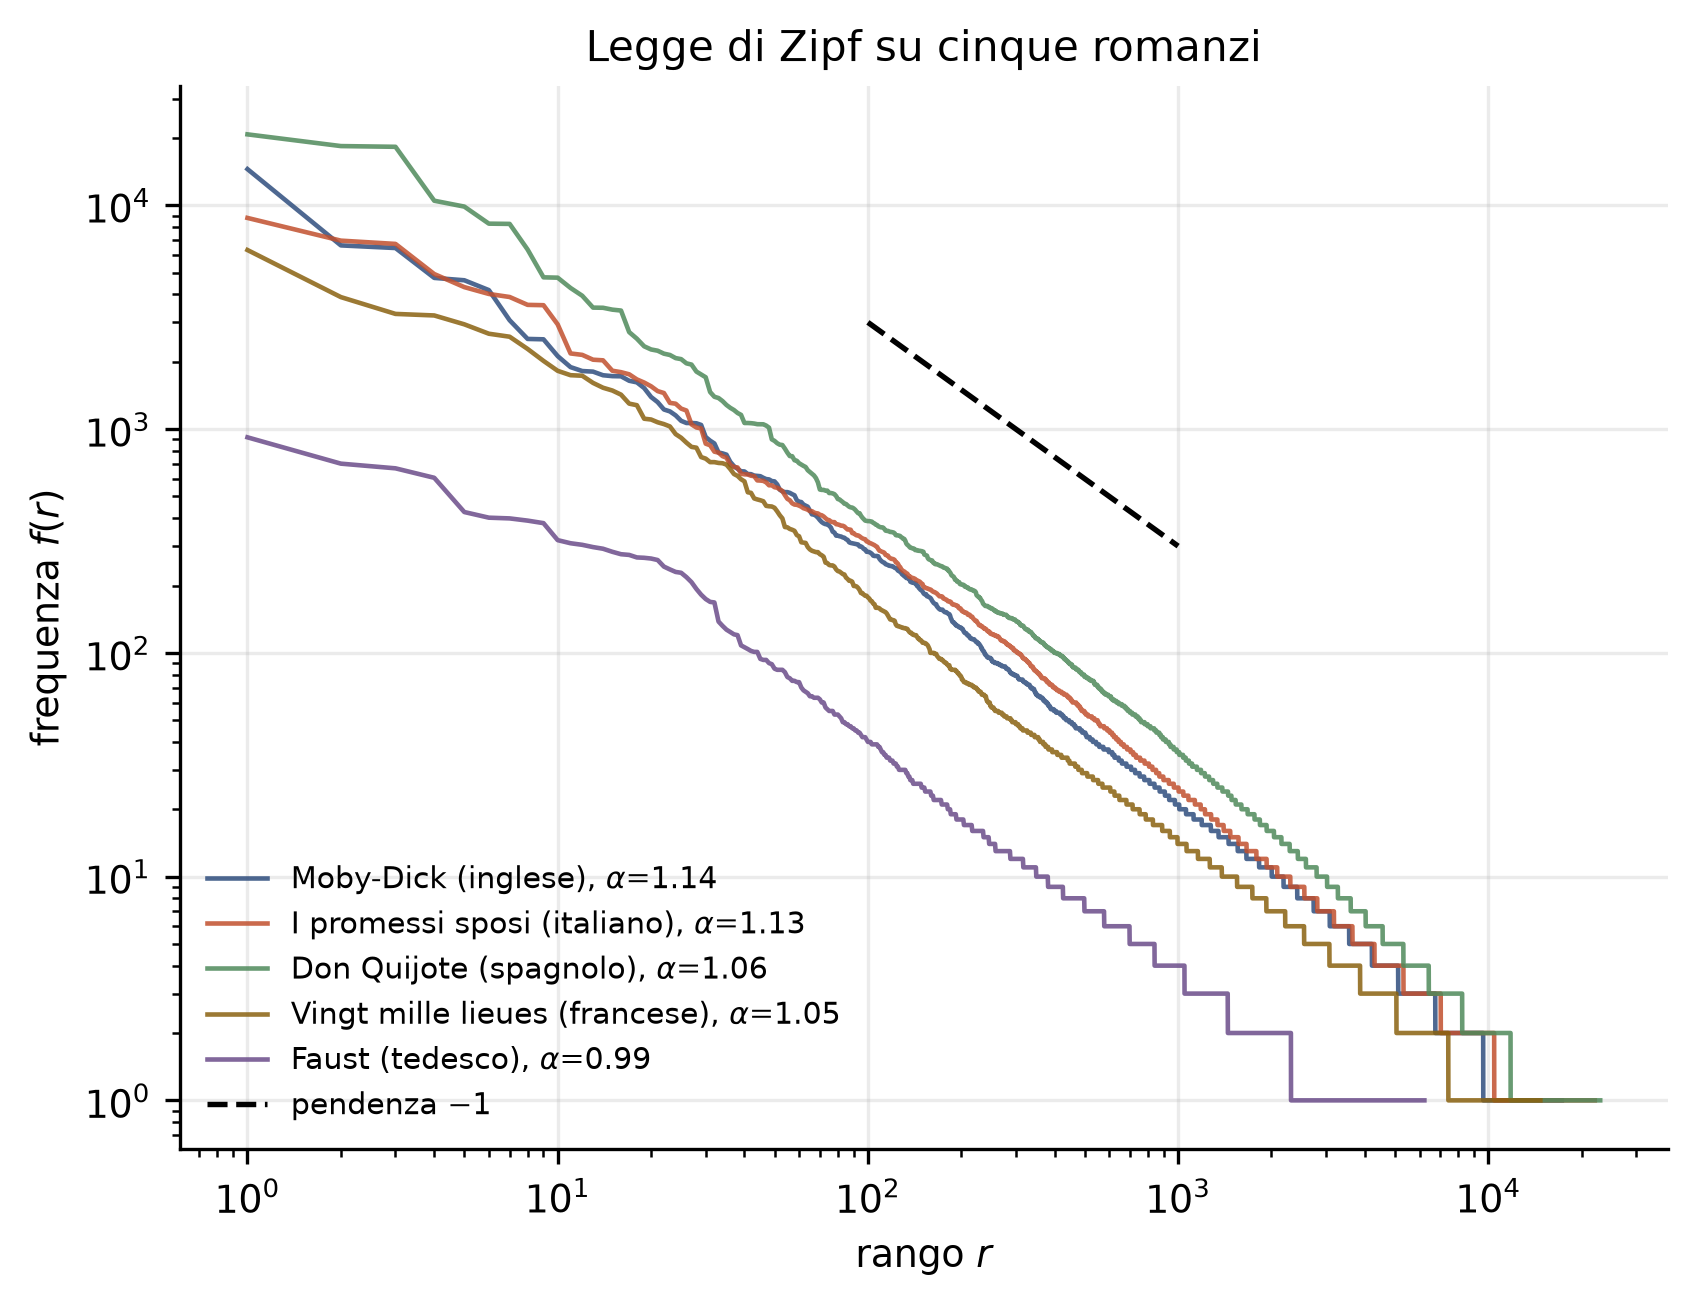
\includegraphics[width=0.82\textwidth]{figure/cap2_zipf_lingue.png}
  \caption{Relazione rango-frequenza per cinque romanzi in altrettante lingue,
  in coordinate bilogaritmiche. Gli esponenti riportati in legenda sono stimati
  per regressione ai minimi quadrati nella finestra di ranghi
  $10^2 \le r \le 10^3$, la stessa impiegata in~\cite{lippi2019}. La retta
  tratteggiata ha pendenza $-1$ ed è riportata come riferimento visivo.}
  \label{fig:zipf}
\end{figure}

Il parametro $\alpha$ risulta positivo e prossimo a 1 nella grande maggioranza
delle lingue esaminate, comprese quelle estinte e quelle costruite
artificialmente. Valori di
$\alpha$ più alti sono sintomo di un vocabolario più povero, poiché un numero
minore di parole esaurisce la maggior parte del testo; valori più bassi
segnalano al contrario una presenza più marcata di parole rare.

I valori misurati sulle cinque opere della Figura~\ref{fig:zipf} sono raccolti
nella Tabella~\ref{tab:zipf-misure}, accanto ai valori medi per lingua riportati
in~\cite{mikhaylovskiy2025zipf} su un corpus di sei opere letterarie in cinque
lingue.

\begin{table}[htbp]
\centering
\small
\begin{tabular}{@{}llrrr@{}}
\toprule
Opera & Lingua & Parole & $|\mathcal{D}|$ & $\alpha$ \\
\midrule
Moby-Dick               & inglese   & \num{219081} & \num{17258} & 1.14 \\
I promessi sposi        & italiano  & \num{239353} & \num{22040} & 1.13 \\
Don Quijote             & spagnolo  & \num{383633} & \num{22943} & 1.06 \\
Vingt mille lieues sous les mers & francese & \num{148923} & \num{14716} & 1.05 \\
Faust                   & tedesco   & \num{30959}  & \num{6221}  & 0.99 \\
\bottomrule
\end{tabular}
\caption{Esponente di Zipf misurato sulle cinque opere della
Figura~\ref{fig:zipf}, con il numero di occorrenze e la dimensione del
dizionario. La stima è condotta sui ranghi $10^2$--$10^3$.}
\label{tab:zipf-misure}
\end{table}

\begin{table}[htbp]
\centering
\small
\begin{tabular}{@{}lcccc@{}}
\toprule
& \multicolumn{2}{c}{$\alpha$ (Zipf)} & \multicolumn{2}{c}{$\gamma_H$ (Heaps)} \\
\cmidrule(lr){2-3}\cmidrule(lr){4-5}
Lingua & parole & token & parole & token \\
\midrule
inglese  & $0.952 \pm 0.072$ & $0.985 \pm 0.054$ & $0.809 \pm 0.027$ & $0.802 \pm 0.024$ \\
tedesco  & $0.959 \pm 0.054$ & $1.024 \pm 0.042$ & $0.846 \pm 0.031$ & $0.793 \pm 0.028$ \\
russo    & $1.043 \pm 0.077$ & $1.009 \pm 0.067$ & $0.916 \pm 0.049$ & $0.805 \pm 0.025$ \\
spagnolo & $0.962 \pm 0.030$ & $1.016 \pm 0.035$ & $0.842 \pm 0.025$ & $0.798 \pm 0.028$ \\
francese & $0.963 \pm 0.033$ & $0.989 \pm 0.042$ & $0.843 \pm 0.020$ & $0.801 \pm 0.018$ \\
\bottomrule
\end{tabular}
\caption{Esponenti medi per lingua riportati in~\cite{mikhaylovskiy2025zipf},
misurati su sei opere letterarie per ciascuna lingua, a livello di parola e di
token. In quel lavoro $\alpha$ è stimato sulla rappresentazione
cumulata della distribuzione anziché sulla relazione rango-frequenza; i due
stimatori coincidono soltanto nel limite $\alpha \to 1$, e i valori non vanno
quindi confrontati direttamente con quelli della
Tabella~\ref{tab:zipf-misure}.}
\label{tab:zipf-letteratura}
\end{table}

Sui testi reali si osservano deviazioni sistematiche dalla~\eqref{eq:zipf}. Su
corpora molto ampi l'esponente resta prossimo a 1 soltanto per le prime migliaia
di parole, mentre la coda continua a seguire una legge di potenza ma con
esponente maggiore~\cite{piantadosi2014}. Le parole più frequenti, inoltre,
mostrano frequenze leggermente inferiori a quelle previste: una deviazione che
Mandelbrot~\cite{mandelbrot1953} corregge introducendo un termine additivo nel
rango,
\begin{equation}
  f(r) \;\propto\; (r + c)^{-\alpha},
  \label{eq:mandelbrot}
\end{equation}
dove la costante $c > 0$ attenua la divergenza della legge di potenza ai ranghi
più bassi, spostando di fatto l'origine dell'asse dei ranghi e rendendo il fit
aderente anche nella regione delle parole più comuni.

\paragraph{Bontà del fit.}
Come si vedrà nei capitoli sperimentali, sui testi generati automaticamente
l'aderenza alla legge di potenza non è garantita. Il solo esponente non è
sufficiente a stabilirla, perché descrive la pendenza media della curva e non la
sua forma: una curva marcatamente incurvata in coordinate bilogaritmiche può
avere la stessa pendenza media di una retta, e restituire quindi un valore di
$\alpha$ del tutto ordinario pur non essendo una legge di potenza. Occorre
perciò una seconda quantità, che misuri quanto i dati si discostino dalla retta
interpolante.

Seguendo~\cite{mikhaylovskiy2025zipf}, la qualità del fit viene stimata con
l'errore percentuale assoluto medio
\begin{equation}
  \mathrm{MAPE} \;=\; \frac{1}{n}\sum_{i=1}^{n}
  \left| \frac{y_i - \hat{y}_i}{y_i} \right|,
  \label{eq:mape}
\end{equation}
dove $n$ è il numero di punti su cui è condotta la regressione, $y_i$ il valore
osservato e $\hat{y}_i$ quello previsto dalla retta interpolante in
corrispondenza dello stesso rango. Il MAPE è nullo per dati perfettamente
allineati e cresce al crescere della distanza relativa dalla retta;
essendo definito su scarti relativi, non dipende dall'unità di misura né
dall'ampiezza delle frequenze, e resta quindi confrontabile fra testi di
lunghezza diversa.

Sul corpus di testi letterari usato in~\cite{mikhaylovskiy2025zipf} il MAPE vale
in media $0.156$ con deviazione standard $0.077$. Nei capitoli sperimentali il
suo minimo in funzione della temperatura di generazione individuerà il regime in
cui il testo prodotto è più vicino a una legge di potenza.

% ---------------------------------------------------------------------
\subsection{Legge di Heaps}
\label{sec:heaps}

Studiando l'andamento di $|\mathcal{D}(t)|$ nei testi letterari emerge una
seconda regolarità, nota come legge di Heaps o, dal nome di chi la formulò per
primo~\cite{herdan1964}, di Herdan--Heaps:
\begin{equation}
  |\mathcal{D}(t)| \;\propto\; t^{\gamma_H}, \qquad \gamma_H \in [0,1] .
  \label{eq:heaps}
\end{equation}
Qui $t$ è la posizione nel testo, misurata in numero di parole,
$|\mathcal{D}(t)|$ la dimensione del dizionario parziale e $\gamma_H$
l'esponente di Heaps. I due estremi dell'intervallo corrispondono a due
comportamenti limite: $\gamma_H = 0$ descrive un dizionario che cessa di
crescere, cioè un testo che non introduce più parole nuove, mentre
$\gamma_H = 1$ descrive un dizionario che cresce proporzionalmente alla
lunghezza, cioè un testo in cui ogni parola è nuova. Poiché il dizionario non
può crescere più rapidamente del testo che lo contiene, si ha necessariamente
$|\mathcal{D}(t)| \le t$, e l'esponente non può eccedere l'unità.

La legge di Heaps quantifica dunque la capacità di un testo di rinnovare il
proprio vocabolario, ed è per questo particolarmente istruttiva se si torna alla
Tabella~\ref{tab:tre-regimi} del Capitolo~\ref{cap:introduzione}. Il primo
esempio, monotono e ripetitivo, cessa rapidamente di accrescere il dizionario;
l'ultimo, in cui i caratteri sono estratti a caso, produce quasi soltanto parole
nuove e fa crescere il dizionario senza saturare. La Figura~\ref{fig:heaps}
mostra le curve dei due casi limite accanto a quelle di tre testi letterari.

\begin{figure}[htbp]
  \centering
  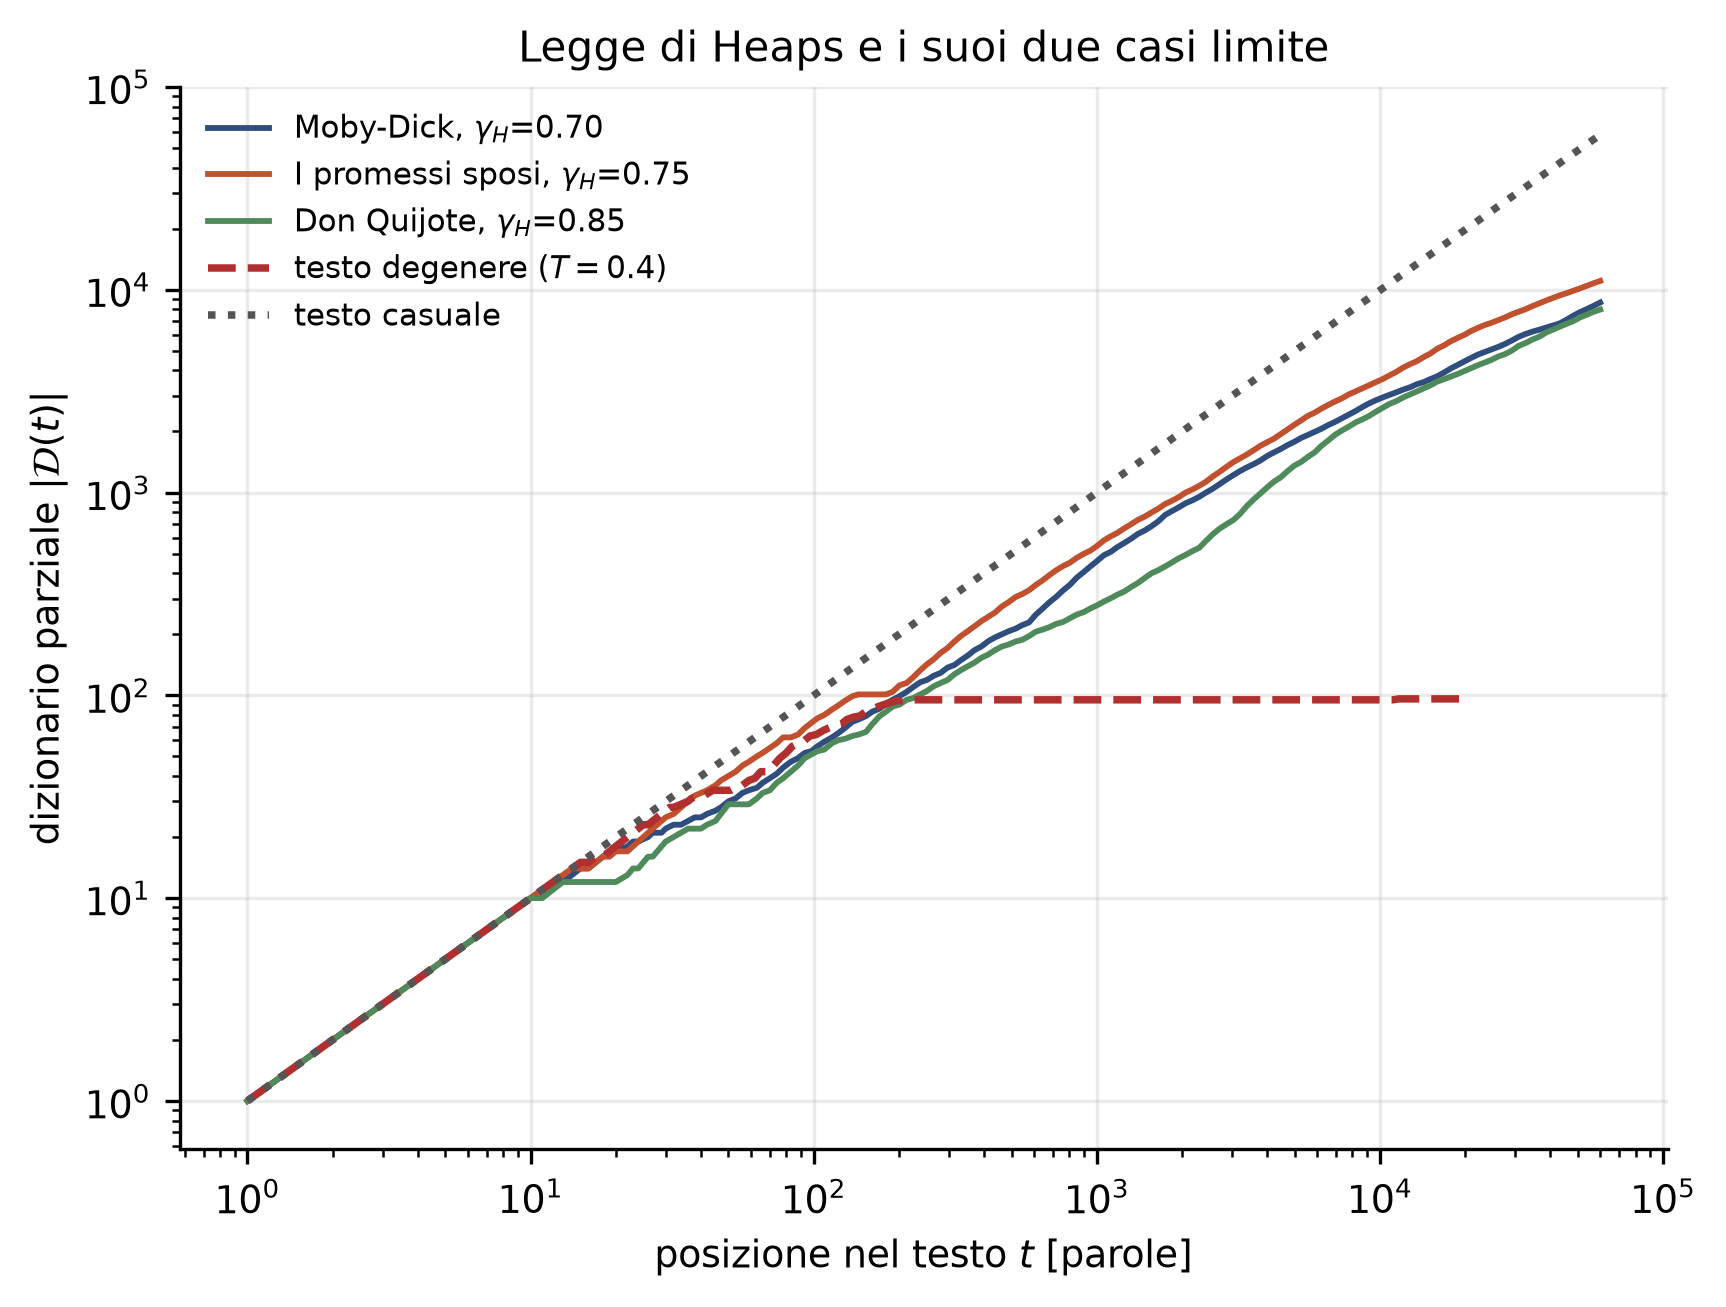
\includegraphics[width=0.82\textwidth]{figure/cap2_heaps_confronto.png}
  \caption{Crescita del dizionario parziale in coordinate bilogaritmiche. Le tre
  curve continue sono testi letterari, con esponente stimato nella regione
  $t > 1000$. La curva tratteggiata è il campione generato a $T = 0.4$ già
  riportato nella Tabella~\ref{tab:tre-regimi}: dopo circa un centinaio di
  parole entra in un ciclo di ripetizione e il dizionario si arresta. La curva
  punteggiata è una sequenza di caratteri casuali, in cui ogni parola è nuova e
  la crescita è esattamente lineare.}
  \label{fig:heaps}
\end{figure}

L'esponente stimato dipende inoltre dall'intervallo su cui viene condotta la
regressione, e quindi dalla lunghezza del testo analizzato. La
Figura~\ref{fig:heaps-finito} mostra l'effetto su tre opere: ripetendo la stima
su prefissi via via più lunghi della stessa opera, $\gamma_H$ decresce in modo
sistematico, di oltre un decimo fra $10^4$ e $10^5$ parole. Il fenomeno è la
prima manifestazione degli effetti di dimensione finita discussi in modo
generale nel §\ref{sec:lunghezza}, ed è già segnalato
in~\cite{mikhaylovskiy2025zipf}, dove si osserva che per $\alpha$ prossimo a 1
la crescita del dizionario è descritta meglio dalla forma $t/\ln t$ che da una
pura legge di potenza. Ai valori di $N$ più bassi la regressione si appoggia a
un intervallo troppo corto e può restituire stime superiori a 1, incompatibili
con il limite teorico: è un artefatto della finestra di fit, non una proprietà
del testo.

\begin{figure}[htbp]
  \centering
  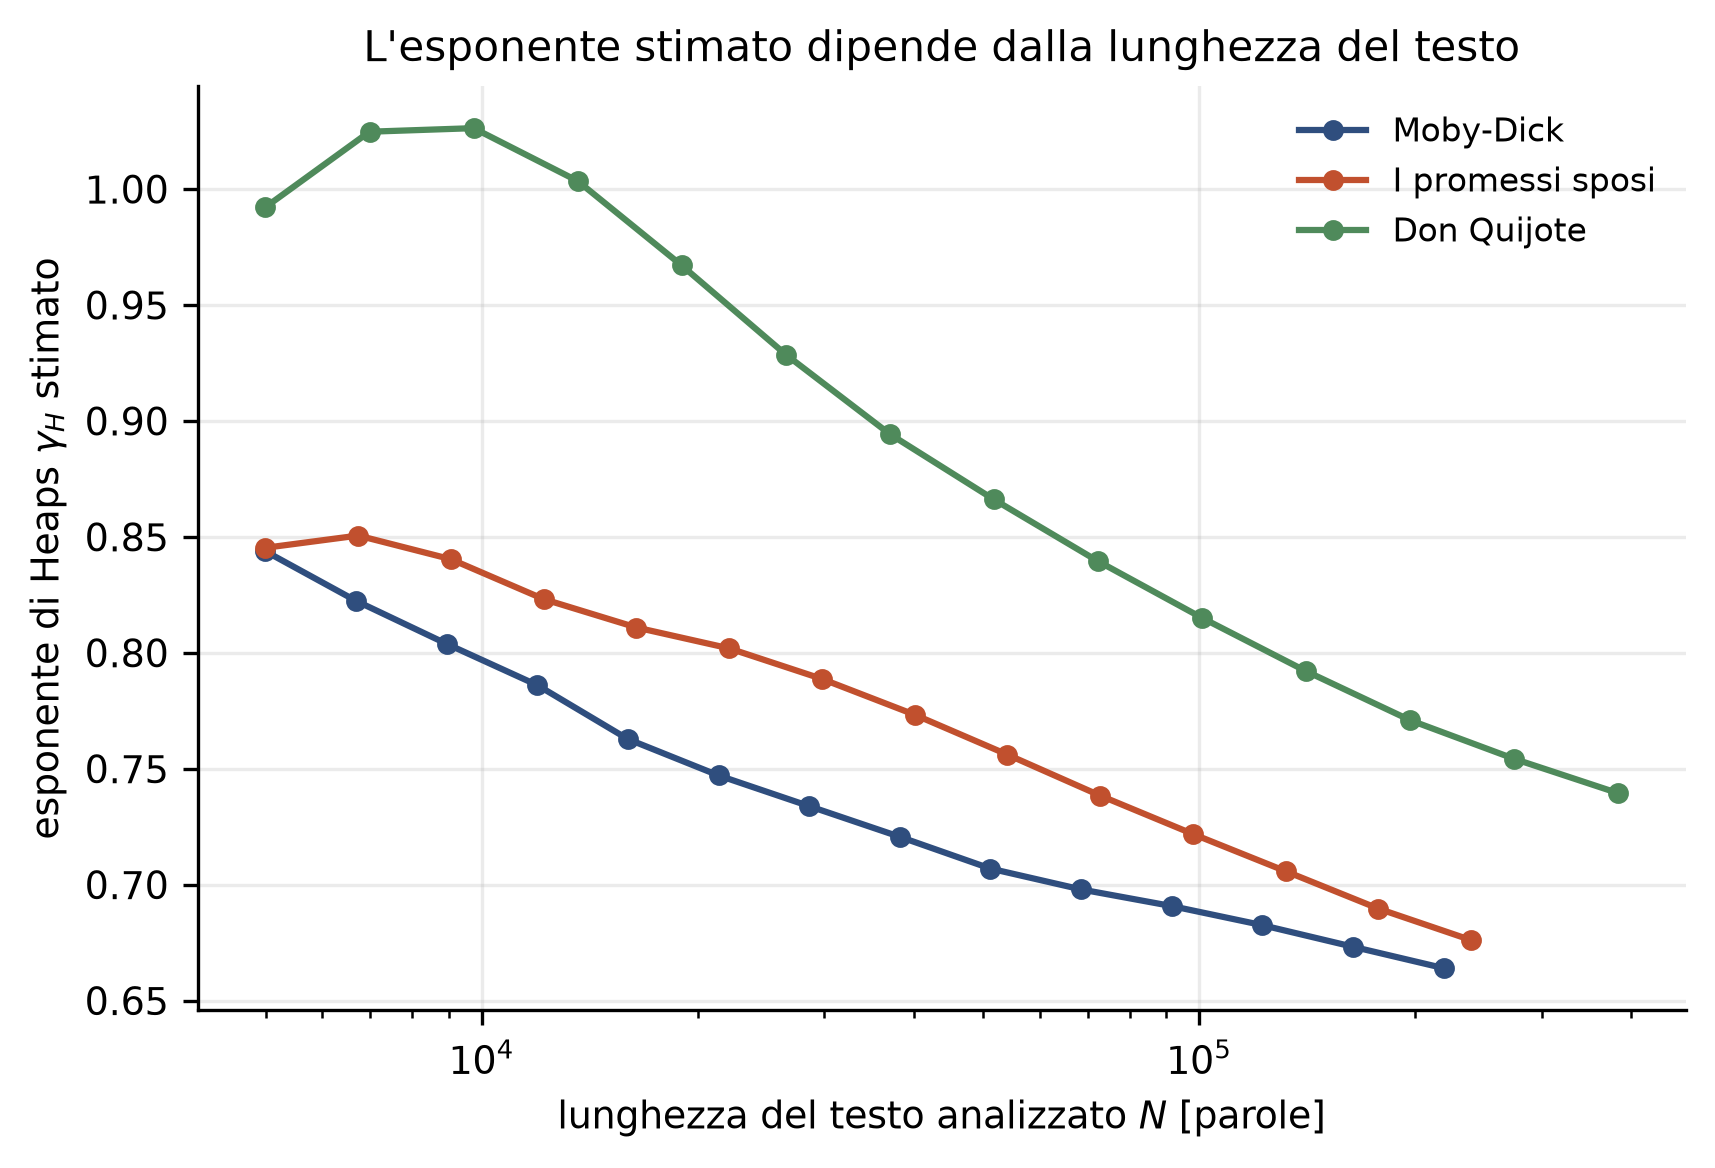
\includegraphics[width=0.78\textwidth]{figure/cap2_heaps_dimensione_finita.png}
  \caption{Esponente di Heaps stimato su prefissi di lunghezza crescente, per tre
  opere in tre lingue diverse, con regressione condotta nella regione $t > 1000$.
  La deriva è sistematica e comune a tutte e tre, ed è quindi una proprietà dello
  stimatore e non di una particolare opera: confrontare esponenti misurati su
  testi di lunghezza diversa non è lecito. Il §\ref{sec:scelte} riprende
  l'effetto su una sola opera, misurandone però l'entità su tutti gli stimatori
  impiegati in questa tesi.}
  \label{fig:heaps-finito}
\end{figure}

\paragraph{Il descrittore $R$.}
Sui testi generati automaticamente la difficoltà è più radicale. A bassa
temperatura di generazione il modello entra in un ciclo di ripetizione e cessa
di produrre parole nuove: la curva $|\mathcal{D}(t)|$ diventa piatta e
la~\eqref{eq:heaps} perde significato. Ad alta temperatura si verifica il caso
opposto, con quasi ogni parola nuova e curva prossima alla linearità. In
entrambe le situazioni la stima di $\gamma_H$ restituisce un numero privo di
contenuto, come mostrano le due curve estreme della Figura~\ref{fig:heaps}.

Per questa ragione in~\cite{mikhaylovskiy2025zipf} viene introdotto un
descrittore che resta definito in ogni regime. Detti $\mathcal{D}_1$ il
dizionario della prima metà del testo e $\mathcal{D}_2$ quello della seconda, si
pone
\begin{equation}
  R \;=\; \frac{|\mathcal{D}_2 \setminus \mathcal{D}_1|}{|\mathcal{D}_1|},
  \label{eq:R}
\end{equation}
cioè il rapporto fra il numero di parole che compaiono per la prima volta nella
seconda metà del testo e il numero di quelle che compaiono per la prima volta
nella prima. Un testo degenerato ha $R$ prossimo a zero, poiché la seconda metà
non introduce nulla di nuovo; un testo in cui ogni parola è nuova ha $R$
prossimo a uno. Sul corpus di opere letterarie intere usato
in~\cite{mikhaylovskiy2025zipf} il valore medio è $R = 0.17$ con deviazione
standard $0.05$.


% ---------------------------------------------------------------------
\section{Correlazioni a lungo raggio}
\label{sec:lrc}

Sia la legge di Zipf sia quella di Heaps ignorano l'ordine dei simboli. Per la
prima l'affermazione è immediata: la~\eqref{eq:zipf} dipende soltanto dai
conteggi delle parole, e un rimescolamento del testo li lascia invariati. Per la
seconda l'invarianza è meno diretta: rimescolando il testo la curva
$|\mathcal{D}(t)|$ cambia realizzazione, perché cambia l'ordine in cui le
parole compaiono per la prima volta, ma il suo andamento medio resta lo stesso, e con esso l'esponente
$\gamma_H$. Entrambe sono quindi proprietà del vocabolario, non della sequenza.

Per misurare le proprietà che dipendono dall'ordine occorre estrarre dal testo
un segnale, cioè una successione finita di valori reali, e studiarne le
correlazioni a scale diverse. La costruzione del segnale non è unica, e ogni
scelta mette in luce aspetti differenti: si può codificare la posizione delle
singole lettere o di classi di lettere, quella delle parole o di classi
grammaticali, oppure la lunghezza delle frasi. In tutti i casi si osserva che il
linguaggio esibisce correlazioni a lungo raggio, con una struttura che si
estende su molti ordini di grandezza~\cite{altmann2012,montemurro2002}.

% ---------------------------------------------------------------------
\subsection{Funzione di autocorrelazione}
\label{sec:acf}

Data una successione $x_1,\dots,x_N$, la funzione di autocorrelazione a distanza
$s$ è
\begin{equation}
  c(s) \;=\; \langle x_n x_{n+s}\rangle
  - \langle x_n\rangle\langle x_{n+s}\rangle ,
  \label{eq:acf}
\end{equation}
dove $\langle\cdot\rangle$ indica la media su tutte le posizioni $n$ compatibili
con la distanza $s$. La forma funzionale di $c(s)$ distingue i regimi di
correlazione.

Se i valori non sono correlati, $c(s)$ è identicamente nulla per $s \neq 0$. Se
$c(s)$ decade esponenzialmente,
$c(s) \sim e^{-s/s_0}$, il segnale si dice correlato a corto raggio: la costante
$s_0$ ha le dimensioni di una distanza e ne fissa la scala caratteristica, nel
senso che oltre poche volte $s_0$ la correlazione è numericamente
indistinguibile da zero. Esiste dunque una distanza tipica oltre la quale due
porzioni di segnale sono indipendenti, e il sistema non possiede struttura al di
là di essa.

Si dice invece che il segnale è correlato a lungo raggio quando il decadimento
segue la legge di potenza
\begin{equation}
  c(s) \;\sim\; s^{-\theta},
  \label{eq:acf-power}
\end{equation}
con $0<\theta<1$. In questo caso non esiste alcuna scala privilegiata: la
funzione~\eqref{eq:acf-power} è invariante di scala, cioè riscalare $s$ di un
fattore costante riscala $c$ di un fattore costante senza modificarne la forma,
e un certo grado di correlazione persiste a tutte le distanze.\footnote{L'esponente
qui indicato con $\theta$ è denotato con $\beta$ in~\cite{altmann2012} e con
$\gamma$ in altra parte della letteratura. Il simbolo è stato cambiato per
evitare la collisione con l'esponente di Heaps e con quello introdotto
nella~\eqref{eq:sigma}.}

La stima diretta di $\theta$ dalla~\eqref{eq:acf-power} è però problematica. Il
segnale è affetto da rumore e, soprattutto, da tendenze di origine esterna che
non sono oggetto di interesse: se la media $\langle x_n\rangle$ differisce fra
la prima e la seconda metà del segnale, come accade proprio quando le
correlazioni sono forti, la~\eqref{eq:acf} risulta distorta. L'esponente va
quindi stimato per via indiretta, e le due sottosezioni seguenti presentano i
due metodi impiegati in questa tesi.

% ---------------------------------------------------------------------
\subsection{Indicatore integrato}
\label{sec:integrato}

Il primo metodo è quello adottato da Altmann, Cristadoro e Degli
Esposti~\cite{altmann2012}, e si applica a segnali binari. Sia dato un testo
come successione simbolica $s = (s_1,\dots,s_N)$. Si definisce una condizione
locale $\mathcal{A}$ che genera la successione binaria
\begin{equation}
  x_k \;=\;
  \begin{cases}
    1 & \text{se $\mathcal{A}$ è soddisfatta in posizione $k$},\\
    0 & \text{altrimenti}.
  \end{cases}
  \label{eq:osservabile}
\end{equation}
L'osservabile può essere la presenza di una data lettera, di una data parola,
oppure l'appartenenza a una classe: per esempio se la lettera in posizione $k$ è
una vocale. L'unità di misura della distanza è il numero di simboli del livello
considerato, ed è questa scelta a rendere confrontabili fra loro una successione
di lettere e una di parole.

Posto
\begin{equation}
  X(t) \;=\; \sum_{j \le t} x_j ,
  \label{eq:conteggio}
\end{equation}
cioè il numero di occorrenze osservate nelle prime $t$ posizioni, si studia la
crescita della varianza del conteggio
\begin{equation}
  \sigma_X^2(t) \;=\; \langle X(t)^2\rangle - \langle X(t)\rangle^2
  \;\simeq\; t^{\gamma}, \qquad \gamma = 2 - \theta .
  \label{eq:sigma}
\end{equation}
La quantità $\sigma_X^2$ è, per costruzione, una somma delle correlazioni a
tutte le distanze inferiori a $t$, e come tale è numericamente assai più stabile
della~\eqref{eq:acf} stimata punto per punto.

Il discrimine fra correlazioni a corto e a lungo raggio non è l'ampiezza di
$c(s)$, ma la sua sommabilità. La~\eqref{eq:conteggio} è formalmente il
cammino percorso da un camminatore che a ogni passo avanza di $x_j$: se i passi
sono indipendenti, o abbastanza rapidamente decorrelati perché $\sum_s c(s)$
converga, vale il teorema del limite centrale e la varianza del cammino cresce
proporzionalmente al numero di passi. Si ha allora diffusione normale,
$\gamma = 1$, esattamente come per il moto browniano. Se invece la somma
diverge, cioè se $\theta \le 1$, i passi restano correlati a ogni scala, il
camminatore tende a proseguire nella direzione già intrapresa e si allontana
dall'origine più rapidamente: la diffusione è anomala e $1 < \gamma < 2$. Il
valore $\gamma = 1$ costituisce dunque il riferimento nullo di tutte le misure
di questo tipo.

La stima di $\gamma$ risente di effetti di tempo finito che la fanno
sottostimare~\cite{altmann2012}: tutti i valori riportati nei capitoli
sperimentali vanno letti come limiti inferiori.

% ---------------------------------------------------------------------
\subsection{Detrended fluctuation analysis}
\label{sec:dfa}

Il secondo metodo è la \emph{detrended fluctuation analysis}, introdotta da
Peng et al.~\cite{peng1994} e applicata ai testi generati automaticamente
in~\cite{lippi2019}. Rispetto all'indicatore integrato presenta il vantaggio
di rimuovere le tendenze locali, e risulta quindi applicabile anche a segnali
non stazionari, cioè segnali le cui proprietà statistiche, tipicamente la
media $\langle x_n \rangle$ o la varianza, non sono costanti lungo la
successione ma derivano lentamente da un estremo all'altro.

La distinzione fra tendenza e correlazione è essenziale, e non riguarda solo
l'origine delle due. Una tendenza è una deriva sistematica e regolare del valore
medio, sovrapposta al segnale da una causa esterna al sistema; una correlazione
è invece una proprietà statistica interna, che lega fra loro le fluttuazioni
attorno a quel valore medio. Il problema pratico è che entrambe producono lo
stesso effetto sulla~\eqref{eq:acf}, gonfiandola a grandi distanze, ed è quindi
necessario eliminare le prime per misurare le seconde. Si potrebbe pensare
sufficiente sottrarre una media mobile di ampiezza fissata, ma in questo modo si
introdurrebbe artificialmente nei dati proprio quella ampiezza come scala
caratteristica, distruggendo le altre.

Il segnale viene costruito codificando ogni carattere del testo con il proprio
rango di frequenza: al carattere più frequente si associa 1, al secondo 2, e
così via. Seguendo~\cite{lippi2019} la codifica avviene a livello di carattere e
conserva punteggiatura, cifre, maiuscole e lettere accentate. Ottenuta la
successione $x_i$ con $i = 1,\dots,N$, la procedura si articola in quattro
passi, qui presentati nella formulazione di~\cite{kantelhardt2001}.

\begin{enumerate}
  \item Si determina il profilo
    \begin{equation}
      Y(i) \;=\; \sum_{k=1}^{i}\bigl(x_k - \langle x\rangle\bigr),
      \label{eq:dfa-profilo}
    \end{equation}
    cioè lo scarto cumulato dalla media. La sottrazione della media non è
    strettamente necessaria, poiché verrebbe comunque eliminata dal detrending.
  \item Si divide il profilo in $N_s = \lfloor N/s \rfloor$ segmenti disgiunti
    di lunghezza $s$.
  \item In ciascun segmento si interpola ai minimi quadrati la tendenza locale,
    ottenendo il polinomio $Y_s(i)$ che approssima il profilo entro quel
    segmento. L'ordine del polinomio determina l'ordine delle tendenze rimosse:
    una DFA di ordine $n$ elimina le tendenze polinomiali fino al grado $n$. In
    questa tesi si impiega l'ordine 1, che rimuove le tendenze lineari locali;
    la robustezza dei risultati rispetto a questa scelta è verificata nel
    §\ref{sec:robustezza}.
  \item Si calcola lo scarto quadratico medio del profilo dalla propria
    tendenza locale, mediando su tutti i segmenti, e si ottiene la funzione di
    fluttuazione
    \begin{equation}
      F(s) \;=\; \left(\frac{1}{N}\sum_{i=1}^{N}
      \bigl(Y(i) - Y_s(i)\bigr)^2\right)^{1/2}.
      \label{eq:dfa-F}
    \end{equation}
\end{enumerate}

La fluttuazione cresce con la lunghezza dei segmenti $s$ e, per un segnale
correlato a lungo raggio, segue la legge di potenza
\begin{equation}
  F(s) \;\sim\; s^{\alpha_{\mathrm{DFA}}} .
  \label{eq:dfa-alpha}
\end{equation}
Per un segnale scorrelato, o correlato a corto raggio, si ha
$\alpha_{\mathrm{DFA}} = 1/2$. Valori superiori indicano correlazioni
persistenti: una fluttuazione positiva tende a essere seguita da un'altra
fluttuazione positiva, e il segnale conserva memoria della propria direzione.
Valori inferiori indicano correlazioni antipersistenti, in cui una fluttuazione
positiva tende a essere seguita da una negativa e il segnale tende a tornare
sui propri passi. Un cammino aleatorio dà $\alpha_{\mathrm{DFA}} = 3/2$: i suoi
incrementi sono scorrelati, ma la successione che ne risulta accumula ogni
deviazione senza riassorbirla, e le fluttuazioni crescono di conseguenza molto
più in fretta. Sul testo letterario di riferimento~\cite{lippi2019} riporta
$\alpha_{\mathrm{DFA}} \simeq 0.65$, contro $0.50$ misurato sulla sua versione
rimescolata: nettamente sopra il riferimento scorrelato e nettamente sotto
quello del cammino aleatorio.

% ---------------------------------------------------------------------
\subsection{Relazione fra i due metodi}
\label{sec:ponte}

I due metodi introdotti misurano la stessa proprietà, e i rispettivi esponenti
sono legati da una relazione semplice. Applicata alla medesima successione,
la~\eqref{eq:dfa-F} coincide, a meno del detrending, con la deviazione standard
del profilo alla scala $s$, cioè $F(s) \simeq \sigma_X(s)$. Elevando al quadrato
e usando la~\eqref{eq:sigma} si ottiene $F(s)^2 \simeq s^{\gamma}$, da cui
\begin{equation}
  \alpha_{\mathrm{DFA}} \;=\; \frac{\gamma}{2} \;=\; 1 - \frac{\theta}{2} .
  \label{eq:ponte}
\end{equation}
La stessa relazione, ricavata per altra via, è riportata
in~\cite{kantelhardt2001}. Nella~\eqref{eq:ponte} $\gamma$ è l'esponente di
crescita della varianza del conteggio definito nella~\eqref{eq:sigma}, mentre
$\theta$ è l'esponente di decadimento dell'autocorrelazione definito
nella~\eqref{eq:acf-power}; i tre esponenti sono dunque tre modi equivalenti di
esprimere la stessa proprietà del segnale.

La~\eqref{eq:ponte} costituisce il ponte fra le due parti sperimentali della
tesi: la diffusione normale $\gamma = 1$, riferimento nullo dell'analisi di
burstiness, corrisponde esattamente al valore $\alpha_{\mathrm{DFA}} = 1/2$,
riferimento nullo dell'analisi sui testi generati. Le due misure non coincidono
esattamente sui dati, poiché la detrended fluctuation analysis rimuove le
tendenze locali mentre l'indicatore integrato no; la differenza fra i due
risultati è informativa proprio quando il segnale non è stazionario.

Un caso limite si presenta con frequenza nei testi generati a bassa
temperatura. Se il testo degenera in un ciclo di ripetizione,
la successione $x_i$ diventa quasi periodica e il profilo~\eqref{eq:dfa-profilo}
oscilla invece di allontanarsi dall'origine: la fluttuazione satura oltre la
lunghezza del periodo e $\alpha_{\mathrm{DFA}}$ scende verso zero. Un esponente
molto basso non segnala quindi assenza di struttura, ma struttura periodica, e
va interpretato congiuntamente a un indicatore diretto di ripetizione.


% ---------------------------------------------------------------------
\section{Burstiness e statistica degli intervalli}
\label{sec:burst}

Le sezioni precedenti permettono di stabilire se un testo possieda correlazioni
a lungo raggio. Questa sezione introduce gli strumenti necessari a stabilire
l'origine di tali correlazioni, che è la domanda posta in~\cite{altmann2012} e
ripresa nella seconda parte sperimentale.

Il punto di partenza è un'osservazione elementare sulla distribuzione delle
parole lungo il testo. Non tutte le parole si distribuiscono allo stesso modo:
alcune ricorrono in modo pressoché uniforme dall'inizio alla fine, altre si
addensano nelle sezioni che trattano l'argomento cui appartengono e sono quasi
assenti altrove. La Figura~\ref{fig:barcode} rende visibile la differenza. Ogni
barra verticale segna una posizione in cui la parola compare; nel primo pannello
la parola è un articolo, nel secondo il nome di un personaggio.

\begin{figure}[htbp]
  \centering
  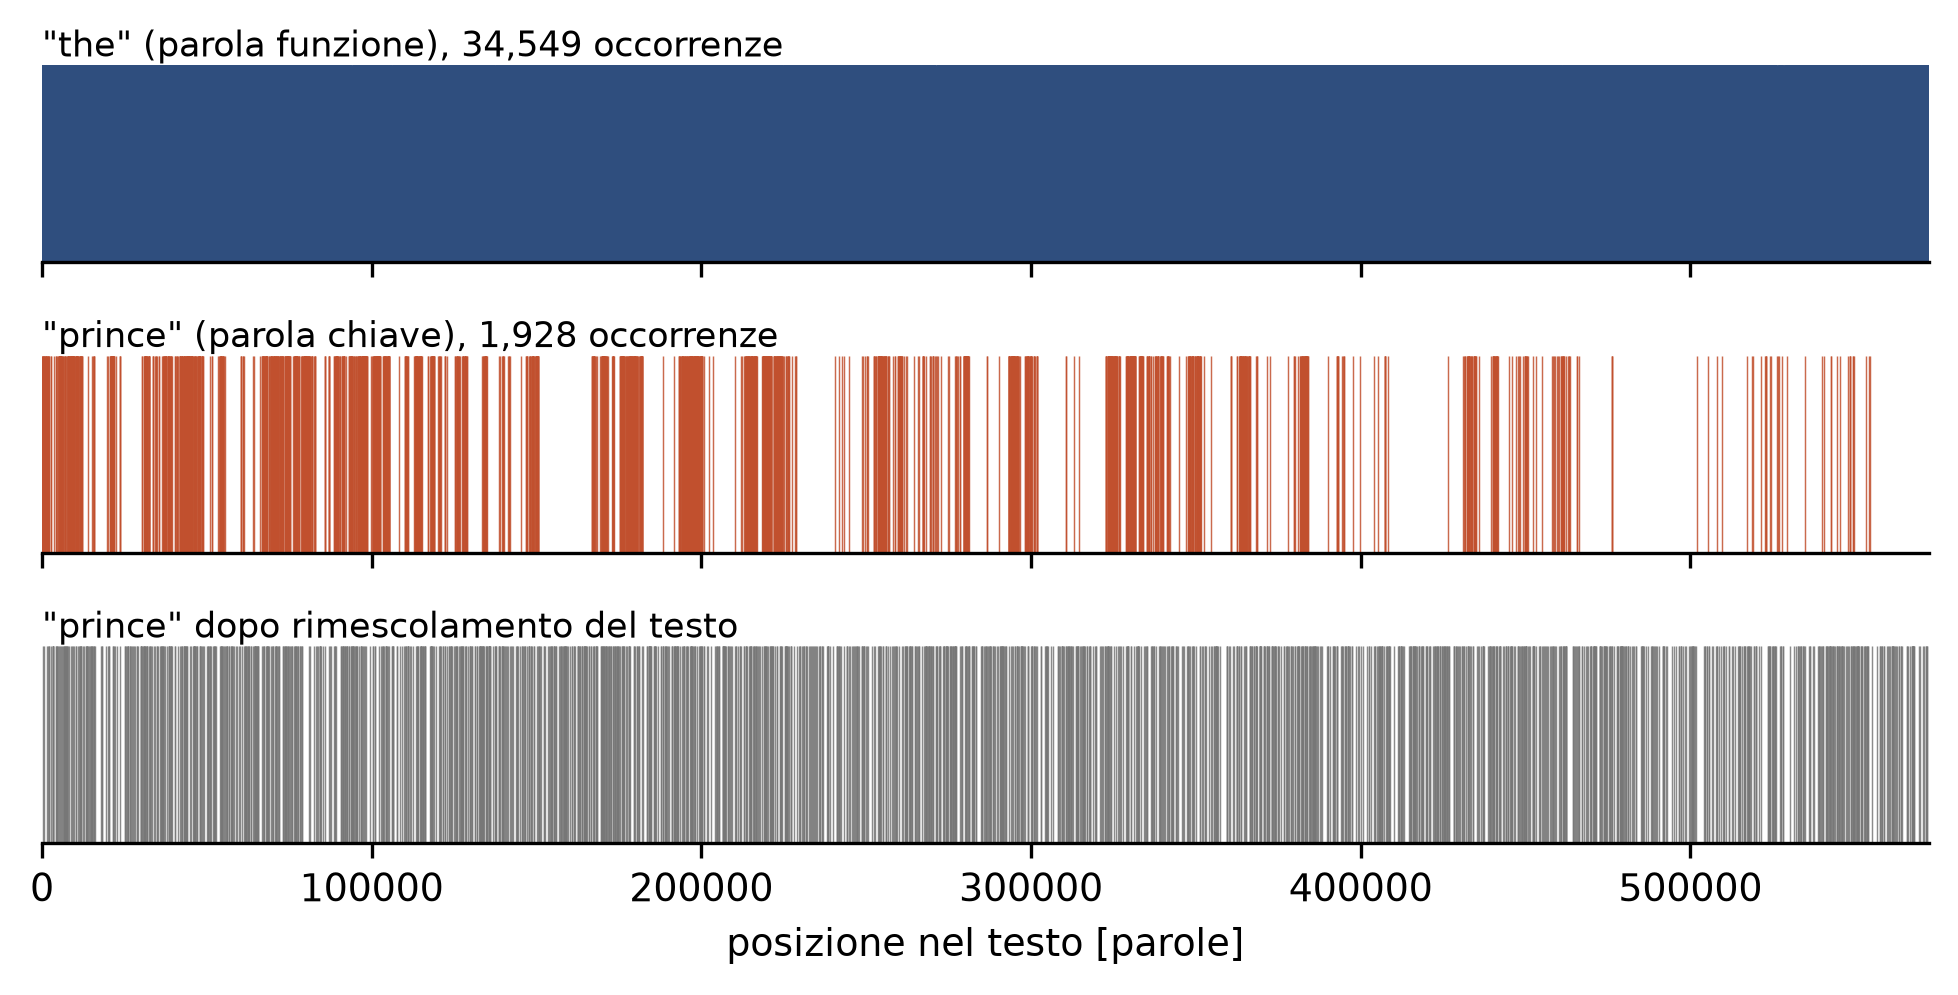
\includegraphics[width=\textwidth]{figure/cap2_burstiness_barcode.png}
  \caption{Posizioni di occorrenza di due parole in \emph{Guerra e pace}. La
  parola funzione \emph{the} riempie il testo in modo uniforme e il pannello
  appare come una banda piena. La parola chiave \emph{prince} si addensa invece
  in gruppi separati da lunghi vuoti, che corrispondono alle porzioni di romanzo
  in cui il personaggio non compare. Il terzo pannello riporta le occorrenze di
  \emph{prince} dopo aver rimescolato le parole del testo: i conteggi sono
  identici, ma i gruppi scompaiono. La struttura visibile nel secondo pannello
  è dunque una proprietà dell'ordine, non delle frequenze.}
  \label{fig:barcode}
\end{figure}

Il fenomeno illustrato dal secondo pannello prende il nome di
\emph{burstiness}: le occorrenze non sono sparse indipendentemente, ma
raggruppate in raffiche separate da intervalli lunghi. Il terzo pannello mostra
perché si tratti di una proprietà dell'ordine e non del vocabolario: il
rimescolamento conserva esattamente il numero di occorrenze, e con esso la legge
di Zipf, ma distrugge la struttura.

Per quantificare il fenomeno si torna alla successione binaria definita
nella~\eqref{eq:osservabile} e si considerano gli intervalli
$\tau_1, \tau_2, \dots$ fra occorrenze consecutive, cioè le distanze in numero
di simboli fra un $1$ e il successivo. La loro distribuzione di probabilità
viene indicata con $p(\tau)$ ed è l'oggetto centrale di questa sezione: tutta
l'informazione sull'ordine che il conteggio delle occorrenze non cattura è
contenuta in $p(\tau)$ e nelle correlazioni fra intervalli successivi.

Il termine di paragone naturale è il processo di Poisson, cioè il processo in
cui ogni posizione ha la stessa probabilità di ospitare un'occorrenza,
indipendentemente da tutte le altre. È il modello del «nessuna struttura»: se le
occorrenze di \emph{prince} fossero poissoniane, il secondo pannello della
Figura~\ref{fig:barcode} sarebbe indistinguibile dal terzo. Per un processo di
Poisson gli intervalli sono distribuiti esponenzialmente e indipendenti fra
loro, e si dimostra che la loro deviazione standard eguaglia la media,
$\sigma_\tau = \langle\tau\rangle$.

Si misura quindi la burstiness con il coefficiente di variazione
\begin{equation}
  \mathrm{cv} \;=\; \frac{\sigma_\tau}{\langle\tau\rangle},
  \label{eq:cv}
\end{equation}
pari a 1 nel caso poissoniano, maggiore di 1 quando le occorrenze si addensano
in raffiche separate da vuoti lunghi e minore di 1 quando sono distribuite in
modo più regolare di quanto il caso comporti. Una misura equivalente, ma
limitata all'intervallo $[-1,1]$ e quindi più comoda per il confronto fra
sequenze diverse, è l'indice proposto da Goh e Barabási~\cite{goh2008},
\begin{equation}
  B \;=\; \frac{\sigma_\tau - \langle\tau\rangle}
                {\sigma_\tau + \langle\tau\rangle} .
  \label{eq:goh}
\end{equation}

% ---------------------------------------------------------------------
\subsection{Le due origini delle correlazioni}
\label{sec:origini}

Il contributo centrale di~\cite{altmann2012} consiste nell'osservare che una
varianza del conteggio che cresce più che linearmente può avere due origini
distinte. Il legame è fornito dallo spettro di potenza a frequenza nulla.

Lo spettro di potenza $S(\omega)$ di una successione descrive come la sua
varianza si distribuisce fra le diverse frequenze $\omega$, ed è la trasformata
di Fourier della funzione di autocorrelazione. Il valore a frequenza nulla,
$S(0)$, raccoglie il contributo delle fluttuazioni più lente, quelle su scale
comparabili con la lunghezza dell'intera successione: è quindi la quantità che
diverge esattamente quando esistono correlazioni a lungo raggio, e che resta
finita quando le correlazioni sono sommabili. Per una successione di occorrenze
descritta dagli intervalli $\tau_i$ vale
\begin{equation}
  S(0) \;=\; \frac{\sigma_\tau^2}{\langle\tau\rangle^3}
  \left(1 + 2\sum_{k\ge1} c_\tau(k)\right),
  \label{eq:eq4}
\end{equation}
dove $c_\tau(k)$ è l'autocorrelazione della successione degli intervalli, cioè
la correlazione fra $\tau_i$ e $\tau_{i+k}$.

La~\eqref{eq:eq4} è il perno dell'intera analisi, perché mostra che $S(0)$ può
divergere in due modi indipendenti. Il primo è la divergenza di $\sigma_\tau$,
cioè una coda pesante di $p(\tau)$: il testo contiene vuoti così lunghi che la
varianza degli intervalli non converge. Il secondo è la non sommabilità di
$c_\tau(k)$, cioè il fatto che gli intervalli siano essi stessi correlati fra
loro. Nella formula resta implicito che cosa questo comporti: $c_\tau(k) > 0$
significa che a un intervallo più lungo della media tende a seguirne un altro
più lungo della media, e quindi che i vuoti si
raggruppano fra loro invece di alternarsi ai riempimenti. Anche con una
$p(\tau)$ a varianza finita, un simile raggruppamento produce fluttuazioni
lente del conteggio e fa divergere la somma.

I due meccanismi sono distinti, perché l'uno riguarda quanto sono lunghi i
vuoti e l'altro come sono disposti, e la~\eqref{eq:eq4} da sola non li separa.

Nei testi reali, di lunghezza finita e con la coda tagliata
(§\ref{sec:coda}), nessuna delle due quantità diverge davvero: ciò che si
misura sono i loro analoghi a finestra finita, e i due null model del
§\ref{sec:null} servono appunto a separarli senza dover decidere quale delle
due divergenze sarebbe realizzata nel limite.

% ---------------------------------------------------------------------
\subsection{I null model A1 e A2}
\label{sec:null}

La separazione si ottiene con due rimescolamenti controllati, costruiti in modo
da distruggere selettivamente uno solo dei due meccanismi.

Il primo, indicato con A1, permuta gli zeri e gli uni della successione binaria.
Conserva soltanto il numero di occorrenze e distrugge tanto la coda di $p(\tau)$
quanto $c_\tau(k)$: è il rimescolamento già illustrato nel terzo pannello della
Figura~\ref{fig:barcode}. Ha funzione di controllo, poiché il risultato è noto a
priori: deve restituire un esponente $\hat\gamma_{A1}$ prossimo a 1, e un valore
diverso segnala un difetto della procedura di misura prima ancora che una
proprietà dei dati.

Il secondo, indicato con A2, permuta fra loro gli intervalli $\tau_i$ senza
alterarne l'insieme. Conserva quindi esattamente $p(\tau)$, e con essa
$\sigma_\tau$, ma distrugge ogni correlazione fra intervalli successivi.
L'esponente risultante $\hat\gamma_{A2}$ isola dunque il solo contributo della
burstiness.

Poiché A2 rimuove un contributo che è di norma non negativo, ci si attende la
disuguaglianza
\begin{equation}
  \hat\gamma \;\ge\; \hat\gamma_{A2},
  \label{eq:disug1}
\end{equation}
che in~\cite{altmann2012} è riportata come regolarità empirica, non come
conseguenza necessaria, e che il §\ref{sec:coda-risultati} verifica
direttamente su tutti i corpora. Fornisce quindi un ulteriore controllo interno
alla misura. Risulta naturale
definire la quota di burstiness
\begin{equation}
  q \;=\; \frac{\hat\gamma_{A2} - 1}{\hat\gamma - 1},
  \label{eq:quota}
\end{equation}
prossima a 1 quando la correlazione proviene interamente dalla coda di $p(\tau)$
e prossima a 0 quando proviene interamente da $c_\tau(k)$: $q$ misura cioè quale
frazione dell'eccesso di correlazione sia attribuibile alla sola burstiness.

Il denominatore della~\eqref{eq:quota} è però piccolo nei corpora poco
correlati, dove $\hat\gamma$ è di poco superiore a 1, e $q$ risulta di
conseguenza uno stimatore rumoroso. Per questa ragione, in questo lavoro $q$
viene calcolata separatamente per ciascun documento e riassunta con mediana e
quartili anziché come rapporto fra medie: si tratta di una scelta metodologica
adottata qui, non di una prescrizione della letteratura, motivata dal fatto che
il rapporto fra due medie non coincide con la media dei rapporti quando il
denominatore ha varianza comparabile al proprio valore.

% ---------------------------------------------------------------------
\subsection{Coda della distribuzione degli intervalli}
\label{sec:coda}

Il legame quantitativo fra burstiness ed esponente di correlazione richiede una
forma esplicita per $p(\tau)$. Assumendo una legge di potenza pura e intervalli
scorrelati si ottiene
\begin{equation}
  p(\tau) \sim \tau^{-\mu}, \quad c_\tau(k) = \delta(k), \quad 2 < \mu < 3
  \;\Longrightarrow\;
  \gamma = 4 - \mu .
  \label{eq:eq8}
\end{equation}
La condizione $2<\mu<3$ individua il regime in cui la media di $\tau$ esiste ma
la varianza diverge, ed è esattamente il regime in cui la~\eqref{eq:cv} non
converge al crescere della lunghezza del testo.

La legge di potenza pura è però un modello idealizzato, e lo stesso
\cite{altmann2012} lo riconosce nel formulare la~\eqref{eq:eq8}. Scendendo
nella gerarchia linguistica i vuoti lunghi vengono spezzati: una lettera che
compone una parola chiave compare anche in tutte le altre parole del testo, e i
lunghi intervalli in cui la parola chiave è assente si riempiono di occorrenze
dovute ad altre parole. Esiste quindi una lunghezza $\tau_c$ oltre la quale gli
intervalli, semplicemente, non si osservano più: è il cut-off che quel lavoro
introduce con questo stesso argomento, senza però stimarlo. Il modello
realistico è la legge di potenza troncata
\begin{equation}
  p(\tau) \;\sim\; \tau^{-\mu}\,e^{-\tau/\tau_c},
  \label{eq:troncata}
\end{equation}
che ha due vantaggi rispetto alla forma pura. Il primo è descrittivo: separa due
proprietà distinte della coda, la pendenza $\mu$ nella regione intermedia e la
distanza $\tau_c$ alla quale la coda viene tagliata, mentre un fit con la sola
legge di potenza le confonde in un unico esponente apparente. Il secondo è che
rende la distribuzione normalizzabile e a varianza finita per ogni $\mu$,
eliminando la necessità di assumere $2<\mu<3$. In presenza di cut-off la
burstiness contribuisce solo per distanze inferiori a $\tau_c$, e
la~\eqref{eq:eq8} non vale più come uguaglianza ma come disuguaglianza,
\[
  \hat\gamma_{A2} \;\le\; 4 - \mu ,
\]
che vincola dall'alto l'esponente misurato sul null model A2.

Nella~\eqref{eq:troncata} $\mu$ e $\tau_c$ agiscono sulla forma della coda in
modo parzialmente sovrapposto: rendere la coda più ripida aumentando $\mu$
produce quasi lo stesso effetto che tagliarla prima riducendo $\tau_c$. Di
conseguenza esistono molte coppie $(\mu, \tau_c)$ diverse fra loro che
descrivono i dati quasi altrettanto bene, cioè che rendono quasi identica la
verosimiglianza, la probabilità di osservare i dati raccolti sotto quei valori
dei parametri. La conseguenza pratica è duplice: gli intervalli di confidenza
vanno calcolati per profilo, esplorando cioè la verosimiglianza al variare di
un parametro con l'altro riottimizzato, e non con la formula asintotica che
presuppone parametri indipendenti; e $\mu$ non va riportato separatamente dal
$\tau_c$ che lo accompagna, perché da solo non identifica la coda.

% ---------------------------------------------------------------------
\subsection{Effetti di dimensione finita}
\label{sec:lunghezza}

Per la legge di potenza pura, quando $\mu<3$ la varianza di $p(\tau)$ diverge e
la stima di $\sigma_\tau$ non converge. Con il taglio della~\eqref{eq:troncata}
i momenti sono invece finiti, ma $\tau_c$ è esso stesso una grandezza che
dipende dalla finestra, e la conseguenza osservabile è la medesima:
la~\eqref{eq:cv} cresce monotonamente con la finestra di osservazione,
poiché finestre più lunghe campionano vuoti più lunghi. Lo stesso vale, in
misura diversa, per l'esponente di Heaps e per il MAPE, come già mostrato nella
Figura~\ref{fig:heaps-finito} del §\ref{sec:heaps}.

La deriva non è un difetto di stima che una procedura migliore potrebbe
eliminare: è una proprietà delle quantità stesse, che su una finestra finita non
hanno un valore limite. Ne discendono vincoli su come i confronti possono essere
condotti, ed è il Capitolo~\ref{cap:metodi} a fissarli, insieme alla misura
dell'entità dell'effetto sui corpora effettivamente impiegati.


% ---------------------------------------------------------------------
\subsection{Entropia degli intervalli}
\label{sec:entropia-intervalli-def}

Il coefficiente di variazione della~\eqref{eq:cv} ha due limiti che il
§\ref{sec:lunghezza} rende evidenti. Il primo è la dipendenza dalla lunghezza
di analisi, che ne impedisce il confronto fra corpora misurati su finestre
diverse. Il secondo è più sottile: $\mathrm{cv}$ è un rapporto e quindi non
cambia se tutti gli intervalli vengono moltiplicati per una costante, ma nei
confronti fra corpora la dilatazione non è uniforme. Quando il tempo si conta in
caratteri, un corpus con frasi mediamente più lunghe produce intervalli più
lunghi ai soli livelli definiti su unità linguistiche, e non a quello dei
caratteri: la scala dei $\tau$ non è la stessa nei due corpora e ogni
differenza ne risente.

Serve quindi una misura di irregolarità che dipenda dalla forma della
distribuzione degli intervalli e non dalla loro scala. Si adotta a questo
scopo l'entropia differenziale del logaritmo degli intervalli, stimata per
spaziature d'ordine con lo stimatore di Vasicek~\cite{vasicek1976}, diminuita
di quella che si otterrebbe da un processo di Poisson con lo stesso numero di
eventi e la stessa media: \begin{equation} J \;=\; h(\ln\tau) \;-\;
h_{\mathrm{Poisson}}(n, \langle\tau\rangle). \label{eq:entropia-intervalli}
\end{equation}

Le due operazioni rispondono ai due limiti. Prendere il logaritmo rende $J$
invariante per dilatazione: moltiplicare tutti i $\tau$ per una costante trasla
$\ln\tau$ senza modificarne l'entropia differenziale, cosicché la diversa
lunghezza delle frasi non produce alcun effetto. Sottrarre il valore poissoniano
fissa lo zero sul processo privo di struttura, come per la~\eqref{eq:cv}, ma con
un vantaggio ulteriore: il termine sottratto viene simulato con lo stesso
stimatore e con gli stessi $n$ e $\langle\tau\rangle$ del dato osservato, per
cui il bias dello stimatore si cancella in larga parte nella differenza invece
di sommarsi.

\paragraph{Fin dove l'invarianza tiene.}
L'argomento appena dato riguarda una distribuzione continua. Gli intervalli fra
occorrenze in un testo sono invece numeri interi, e l'arrotondamento agli interi
non commuta con la dilatazione: comprimere una distribuzione fino a intervalli
di poche unità ne cancella la forma, e $J$ ne risente. Il pannello A della
Figura~\ref{fig:invarianza-J} misura l'entità del fenomeno moltiplicando per una
costante gli intervalli generati da una stessa legge. Per
$\langle\tau\rangle \gtrsim 30$ le curve sono piatte entro due centesimi di bit
e l'invarianza tiene; per $\langle\tau\rangle = 5$ una dilatazione di un fattore
cinquanta sposta $J$ di $0.59$ bit. L'invarianza è dunque asintotica nel valore
medio degli intervalli, non esatta.

La distinzione ha una conseguenza pratica sui livelli linguistici. Ai due
livelli lessicali, dove la diversa lunghezza delle frasi si fa sentire,
l'intervallo medio nei corpora del Capitolo~\ref{cap:risultati2} vale fra $340$
e $1900$ caratteri, quindi in pieno regime asintotico. Ai livelli delle lettere e
degli spazi, dove l'intervallo medio scende sotto la decina, i valori di $J$
risentono della quantizzazione e vanno letti come descrittori relativi, validi
per confrontare corpora misurati allo stesso modo e non come distanze assolute
dal processo di Poisson.

Il pannello B della stessa figura verifica la cancellazione del bias facendo
crescere il numero di intervalli da $30$ a $1000$ su cinque leggi di forma nota.
La deriva residua non supera $0.07$ bit su un intervallo in cui $n$ cambia di un
fattore trentatré, ed è massima sulle distribuzioni log-normali. La
cancellazione è quindi buona ma non completa, e differenze di $J$ inferiori a un
decimo di bit fra sequenze di numerosità molto diversa non sono interpretabili.

\begin{figure}[htbp]
  \centering
  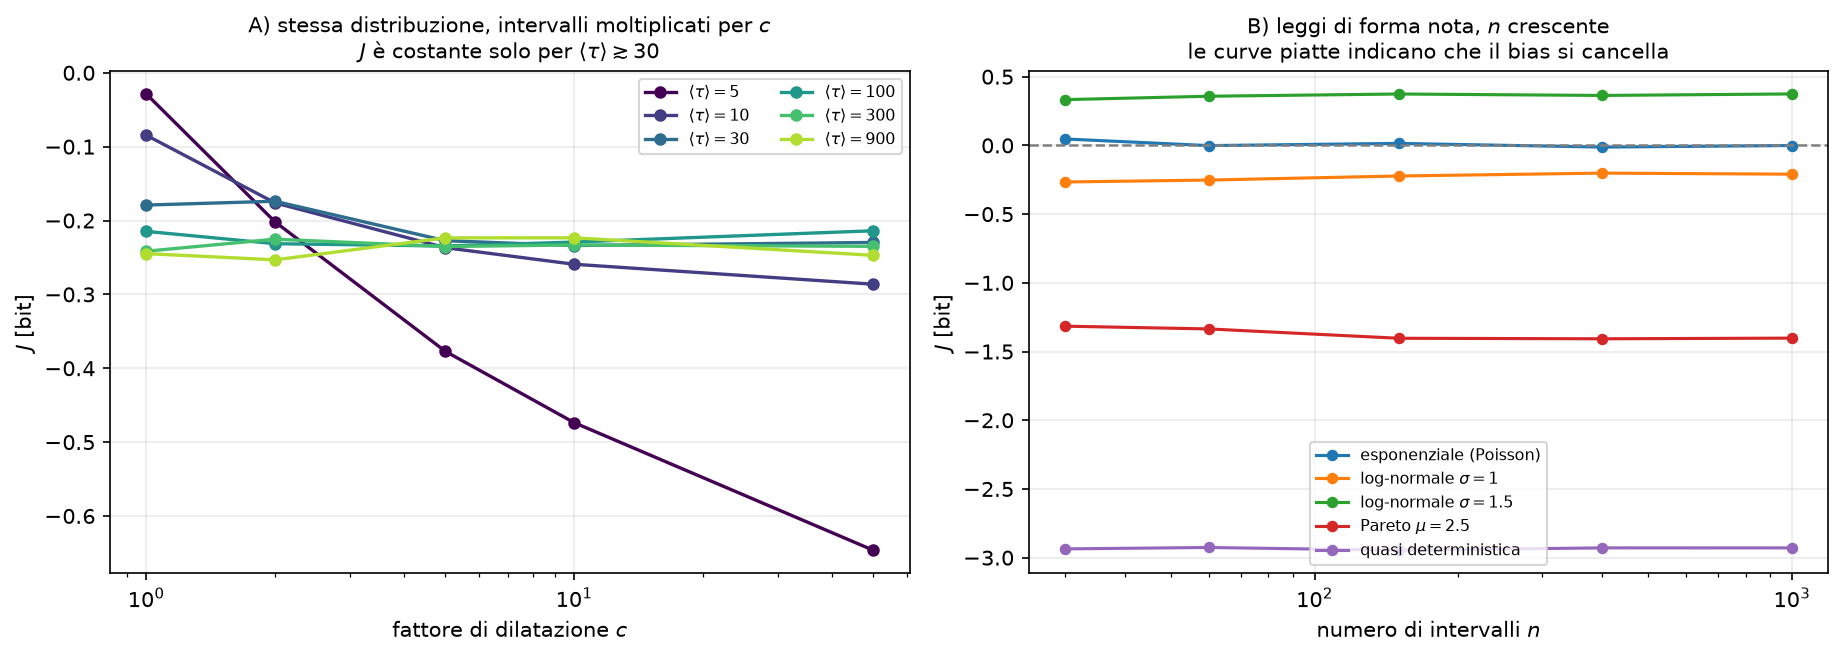
\includegraphics[width=\textwidth]{figure/cap2_invarianza_J.png}
  \caption{Limiti di validità della~\eqref{eq:entropia-intervalli}, misurati
  sullo stimatore effettivamente impiegato. A: intervalli estratti da una stessa
  legge log-normale e moltiplicati per un fattore $c$, per sei valori
  dell'intervallo medio di partenza; una curva piatta indica invarianza. Sotto
  $\langle\tau\rangle \simeq 30$ la quantizzazione agli interi la distrugge. B:
  $J$ su cinque leggi di forma nota al crescere del numero di intervalli; lo
  scostamento fra gli estremi quantifica il bias che la sottrazione del termine
  poissoniano non elimina.}
  \label{fig:invarianza-J}
\end{figure}

Valori positivi di $J$ indicano intervalli distribuiti in modo più irregolare di
un processo di Poisson, valori negativi una regolarità superiore a quella del
caso. La quantità non compare in nessuno dei lavori di riferimento ed è
introdotta qui; il §\ref{sec:entropia-intervalli} ne verifica la stabilità
rispetto alla lunghezza di analisi e la impiega per neutralizzare l'effetto
appena descritto.


% ---------------------------------------------------------------------
\section{Entropia e compressione}
\label{sec:entropia}

Il concetto di disordine di un testo e la nozione di entropia sono già stati
introdotti nel Capitolo~\ref{cap:introduzione}. Trattandosi di un concetto
centrale per questo lavoro, in questa sezione viene definito in modo formale e
ne viene esplicitato il legame con gli algoritmi di compressione, che è lo
strumento con cui l'entropia verrà effettivamente stimata sui testi.

% ---------------------------------------------------------------------
\subsection{Entropia e predicibilità}
\label{sec:entropia-def}

Si consideri una sorgente che emette simboli da un alfabeto finito
$\mathcal{X}$. Per una singola variabile aleatoria $X$ che assume il valore
$x \in \mathcal{X}$ con probabilità $p(x)$, l'entropia di
Shannon~\cite{shannon1948} è
\begin{equation}
  H(X) \;=\; -\sum_{x \in \mathcal{X}} p(x) \log_2 p(x),
  \label{eq:H-singola}
\end{equation}
espressa in bit, e misura l'incertezza media sull'esito dell'estrazione.

I simboli di un testo non sono però indipendenti, e l'entropia di una singola
lettera non descrive la sorgente: sapere che in inglese la lettera più frequente
è \emph{e} dice poco, mentre sapere che dopo \emph{th} segue quasi sempre
\emph{e} dice molto. Occorre quindi considerare blocchi di simboli. Detta
$H(X_1,\dots,X_n)$ l'entropia congiunta di un blocco di lunghezza $n$, definita
dalla~\eqref{eq:H-singola} applicata alla distribuzione congiunta dei blocchi, si
definisce il tasso di entropia della sorgente come
\begin{equation}
  h \;=\; \lim_{n\to\infty} \frac{H(X_1,\dots,X_n)}{n} .
  \label{eq:tasso-entropia}
\end{equation}
Il limite esiste per sorgenti stazionarie ed ergodiche~\cite{cover2006} e
quantifica l'incertezza media per simbolo una volta tenuto conto di tutte le
dipendenze, comprese quelle a lunga distanza. È questa, e non
la~\eqref{eq:H-singola}, la quantità pertinente per un testo.

Il teorema della codifica di sorgente~\cite{cover2006} lega $h$ alla
comprimibilità: il tasso di entropia è un limite inferiore alla lunghezza media
per simbolo di qualunque codifica senza perdita. Stimare l'entropia di un testo
e stimarne la comprimibilità sono quindi, entro le approssimazioni del caso, lo
stesso problema.

Il legame si comprende in modo intuitivo tornando ai casi limite della
Tabella~\ref{tab:tre-regimi}. Un algoritmo di compressione senza perdita opera
sostituendo alle porzioni di testo che si ripetono un riferimento
all'occorrenza precedente, più breve del testo che rimpiazza. Nel testo monotono
il medesimo gruppo di parole ricorre per l'intera lunghezza del documento: dopo
la prima occorrenza tutto il resto è un riferimento, il file compresso è
minuscolo e il tasso di entropia è prossimo a zero, perché il simbolo successivo
è quasi sempre determinato da quelli che lo precedono. Nella sequenza casuale,
al contrario, nessuna porzione si ripete: non esiste nulla cui fare riferimento,
il compressore non guadagna nulla e il tasso di entropia è massimo, perché ogni
simbolo è imprevedibile a partire dai precedenti. Il linguaggio naturale si
colloca fra i due estremi, e la quantità di compressione che ammette è una
misura diretta di quanta struttura possiede.

\paragraph{Stimatori di Lempel--Ziv.}
La stima diretta di $h$ dalla~\eqref{eq:tasso-entropia} per conteggio di blocchi
è impraticabile: il numero di blocchi distinti di lunghezza $n$ cresce
esponenzialmente con $n$, e la dimensione campionaria necessaria a stimarne le
probabilità cresce di conseguenza. Nessun testo reale è abbastanza lungo.

Si ricorre allora agli stimatori della famiglia Lempel--Ziv~\cite{ziv1977},
che aggirano il problema misurando le ripetizioni invece delle probabilità.
L'idea è la seguente: si scorre la successione e, a ogni posizione $i$, si cerca
la più lunga sottostringa che inizi in $i$ e sia già comparsa in precedenza,
detta $\Lambda_i$ la sua lunghezza. In un testo molto ripetitivo i match sono
lunghi, in un testo casuale sono corti. Si dimostra che, per una sorgente
stazionaria ed ergodica, la lunghezza media di tali match cresce come il
logaritmo della finestra esplorata e che
\begin{equation}
  h \;=\; \lim_{n\to\infty}
  \left\langle \frac{\log_2 n}{\Lambda_i} \right\rangle ,
  \label{eq:lz-entropia}
\end{equation}
dove la media è presa sulle posizioni $i$. La~\eqref{eq:lz-entropia} converge
assai più rapidamente del conteggio di blocchi e mantiene buone proprietà anche
in presenza di correlazioni a lungo raggio, che è la ragione per cui viene
adottata qui: le sorgenti considerate in questa tesi hanno, per costruzione,
memoria lunga.

% ---------------------------------------------------------------------
\subsection{Stima della cross-entropia e della divergenza}
\label{sec:crossparsing}

Le quantità introdotte finora descrivono un testo singolo. Per confrontare due
testi occorre la cross-entropia, che misura il costo di codificare un testo
usando la statistica di un altro.

L'algoritmo di cross-parsing di Ziv e Merhav~\cite{ziv1993} estende
la~\eqref{eq:lz-entropia} a due successioni. Data la successione $x$ da
misurare e la successione di riferimento $y$, si scorre $x$ da sinistra a destra
e la si decompone in frasi successive, dove ogni frase è la più lunga
sottostringa che, a partire dalla posizione corrente, compaia da qualche parte
in $y$; raggiunto il punto in cui il match si interrompe, si chiude la frase e
se ne apre una nuova. Il numero di frasi così ottenute viene indicato con
$c(x|y)$ ed è la quantità che misura la somiglianza fra i due testi: se $x$ e
$y$ provengono dalla stessa sorgente, le frasi sono lunghe e poche; se
provengono da sorgenti diverse, i match si interrompono presto e le frasi sono
molte. La stima della cross-entropia è
\begin{equation}
  h(x \,|\, y) \;=\; \frac{c(x|y)\,\log_2 |y|}{|x|},
  \label{eq:crossparsing}
\end{equation}
espressa in bit per simbolo, dove $|x|$ e $|y|$ sono le lunghezze delle due
successioni.

La divergenza di Kullback--Leibler è lo strumento con cui si quantifica quanto
due distribuzioni di probabilità differiscano fra loro. Date due distribuzioni
$P$ e $Q$ sullo stesso alfabeto, essa è definita come
\begin{equation}
  D(P\|Q) \;=\; \sum_{x} P(x) \log_2 \frac{P(x)}{Q(x)}
  \;=\; H_P(Q) - H(P),
  \label{eq:kl-def}
\end{equation}
dove $H_P(Q)$ è la cross-entropia fra le due distribuzioni. La~\eqref{eq:kl-def}
si interpreta come il numero medio di bit sprecati per simbolo codificando una
sorgente $P$ con un codice ottimizzato per $Q$: vale zero se e solo se
$P = Q$ ed è positiva altrimenti.

In termini di successioni, la~\eqref{eq:kl-def} si stima come differenza fra due
cross-entropie: dividendo $x$ in due metà $x_1$ e $x_2$ e prendendo da $y$ un
prefisso $y_1$ della stessa lunghezza di $x_1$, si pone
\begin{equation}
  D(x \,\|\, y) \;=\; h(x_2 \,|\, y_1) \;-\; h(x_2 \,|\, x_1) .
  \label{eq:kl}
\end{equation}
La seconda metà di $x$ viene cioè codificata due volte, una volta usando come
riferimento un testo estraneo e una volta usando la prima metà di $x$ stesso, e
si misura quanto costa in più la prima operazione.

L'appaiamento delle lunghezze dei due riferimenti non è un dettaglio.
La~\eqref{eq:crossparsing} dipende dalla lunghezza del riferimento, poiché un
riferimento più lungo contiene più sottostringhe e produce una cross-entropia
minore a parità di sorgente. Se i due termini della~\eqref{eq:kl} usassero
riferimenti di lunghezza diversa, la differenza conterrebbe un termine spurio
che può superare in modulo il segnale da misurare e produrre stime negative,
impossibili per la~\eqref{eq:kl-def}. Con $|y_1| = |x_1|$ il termine spurio si
cancella, e la costruzione soddisfa la proprietà verificabile $D(x\|x) = 0$
esattamente, impiegata nei capitoli sperimentali come test dello stimatore.

Poiché la~\eqref{eq:kl} non è simmetrica, mentre per confrontare due corpora
serve una quantità che non dipenda da quale dei due venga posto come
riferimento, seguendo~\cite{lippi2019} viene adottata la divergenza
simmetrizzata
\begin{equation}
  D_s(x,y) \;=\; \tfrac{1}{2}\bigl[D(x\|y) + D(y\|x)\bigr].
  \label{eq:kl-sym}
\end{equation}

% ---------------------------------------------------------------------
\subsection{Misure basate su compressione}
\label{sec:compressione}

Le stime della sottosezione precedente usano la compressione come strumento
teorico, attraverso il conteggio delle frasi. Un secondo gruppo di misure,
introdotto in questo contesto da Hadad et al.~\cite{hadad2026}, impiega invece
direttamente un compressore reale come sonda della regolarità strutturale, senza
passare per una stima di entropia.

Detta $C(x)$ la dimensione in byte del testo $x$ dopo la compressione, si
definisce il rapporto di compressione
\begin{equation}
  R_{\mathrm{gzip}}(x) \;=\; \frac{C(x)}{|x|},
  \label{eq:cratio}
\end{equation}
tanto minore quanto più il testo è regolare. Il pedice ricorda l'algoritmo
impiegato e distingue la quantità dal descrittore $R$ della~\eqref{eq:R}.

Da esso derivano la compressione condizionata
$\bigl(C(x+y) - C(x)\bigr)/|y|$, dove $x+y$ indica la concatenazione, che stima
il costo incrementale di codificare la seconda metà di un documento dopo aver
già codificato la prima e misura quindi quanto la seconda metà sia prevedibile
a partire dalla prima; e la distanza normalizzata di compressione~\cite{li2004}
\begin{equation}
  \mathrm{NCD}(x,y) \;=\;
  \frac{C(xy) - \min\{C(x),C(y)\}}{\max\{C(x),C(y)\}} .
  \label{eq:ncd}
\end{equation}
Applicata fra un testo e una sua permutazione, la~\eqref{eq:ncd} misura quanta
parte della comprimibilità dipenda dall'ordine delle parole e non dalla sola
composizione lessicale: è quindi l'analogo, in chiave di compressione, del
confronto fra i pannelli della Figura~\ref{fig:barcode}.


% ---------------------------------------------------------------------
\section{Token ed embedding}
\label{sec:token}

Nel §\ref{sec:scala} si è assunta la parola come unità fondamentale del testo,
in quanto più piccola porzione dotata di significato autonomo per un lettore
umano. Questa scelta non vale più per gli algoritmi di generazione automatica
del testo e, in particolare, per i modelli linguistici di grandi dimensioni.

Si riprenda la frase già usata come esempio,
\emph{Se pensi di comprendere la meccanica quantistica, non comprendi la
meccanica quantistica.} Per un lettore umano essa si scompone come nella
Figura~\ref{fig:scomp-parole}: dodici parole più la punteggiatura, ciascuna
delle quali ha un significato che si può cercare in un dizionario.

\begin{figure}[htbp]
  \centering
  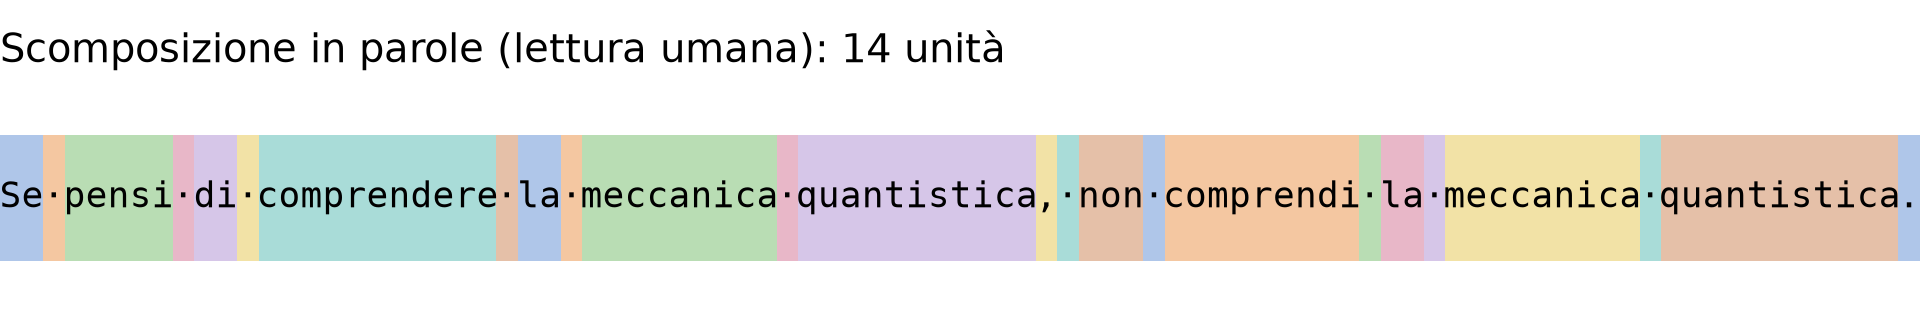
\includegraphics[width=\textwidth]{figure/cap2_scomposizione_parole.png}
  \caption{Scomposizione in parole. Ogni blocco è un'unità dotata di
  significato autonomo; il punto mediano segnala gli spazi.}
  \label{fig:scomp-parole}
\end{figure}

Per un modello linguistico la stessa frase si scompone invece come nella
Figura~\ref{fig:scomp-token}.

\begin{figure}[htbp]
  \centering
  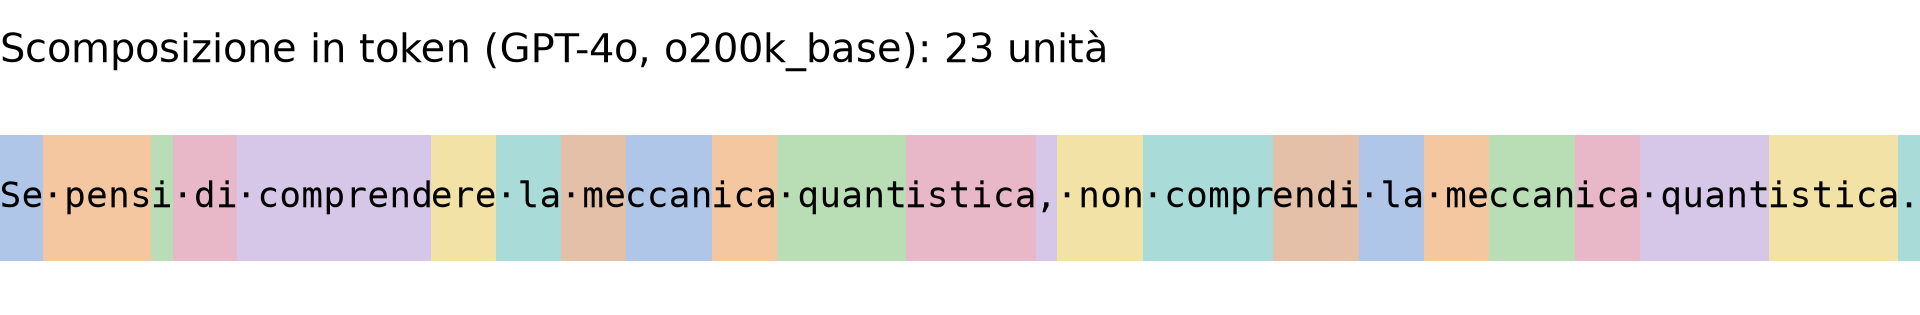
\includegraphics[width=\textwidth]{figure/cap2_scomposizione_token.png}
  \caption{Scomposizione in token della stessa frase, ottenuta con il
  tokenizzatore \texttt{o200k\_base} impiegato da GPT-4o. Le unità sono
  ventitré, non coincidono con le parole e in generale non hanno significato
  autonomo.}
  \label{fig:scomp-token}
\end{figure}

La frase non è divisa né in lettere né in parole, ma in gruppi di lettere
chiamati \emph{token}. Alcuni token coincidono con parole intere
(\texttt{·la}, \texttt{·non}), altri sono frammenti privi di significato
(\texttt{ccan}, \texttt{istica}). Si osservi in particolare la coppia
\emph{comprendere} e \emph{comprendi}: la prima si scompone in
\texttt{·comprend} e \texttt{ere}, la seconda in \texttt{·compr} e
\texttt{endi}. Due forme della stessa radice vengono dunque tagliate in punti
diversi, e il modello non riceve alcuna indicazione esplicita del fatto che
condividano la radice. Lo spazio, inoltre, non separa i token ma vi è
incorporato: la maggior parte dei token inizia con uno spazio, e la
segmentazione del testo in unità precede logicamente qualunque nozione di
parola.

La conversione avviene tramite un algoritmo detto \emph{tokenizzatore}, che
traduce un testo scritto in una qualsiasi lingua e in un qualsiasi alfabeto in
una sequenza di token estratti da un dizionario ampio ma finito, costruito una
volta per tutte a partire da un grande corpus. I dizionari dei tokenizzatori
più diffusi hanno dimensioni dell'ordine di $10^5$ elementi: quello di GPT-4o,
\texttt{o200k\_base}, ne conta \num{200019}; \texttt{cl100k\_base}, impiegato
come unità di analisi nei capitoli sperimentali per le ragioni discusse nel
Capitolo~\ref{cap:metodi}, ne conta \num{100277}; i modelli Qwen2.5 analizzati
in questa tesi ne condividono uno di circa \num{151000} voci. Poiché il
dizionario è finito ma le lingue possibili sono molte, i testi nelle lingue
meno rappresentate nel corpus di costruzione vengono frammentati in un numero
di token assai maggiore rispetto all'inglese.

Proprio come le parole per gli esseri umani, per un modello linguistico sono i
token a trasportare significato. Il significato non è però un'etichetta
associata al token, bensì una posizione: tramite un'operazione detta
\emph{embedding} ogni token viene mappato in un vettore di uno spazio a molte
dimensioni, e la geometria di quello spazio codifica le relazioni fra i token.
Vettori vicini corrispondono a token che compaiono in contesti simili, e
direzioni ricorrenti nello spazio corrispondono a relazioni ricorrenti nel
linguaggio.

La Figura~\ref{fig:embedding} mostra la proprietà su un caso concreto. I vettori
di trenta parole inglesi, appartenenti a cinque famiglie semantiche, sono
proiettati sulle prime due componenti principali dello spazio: le parole di
ciascuna famiglia si dispongono in gruppi distinti, benché la costruzione dei
vettori non abbia mai fatto uso di alcuna classificazione semantica, ma soltanto
delle co-occorrenze osservate in un corpus.

\begin{figure}[htbp]
  \centering
  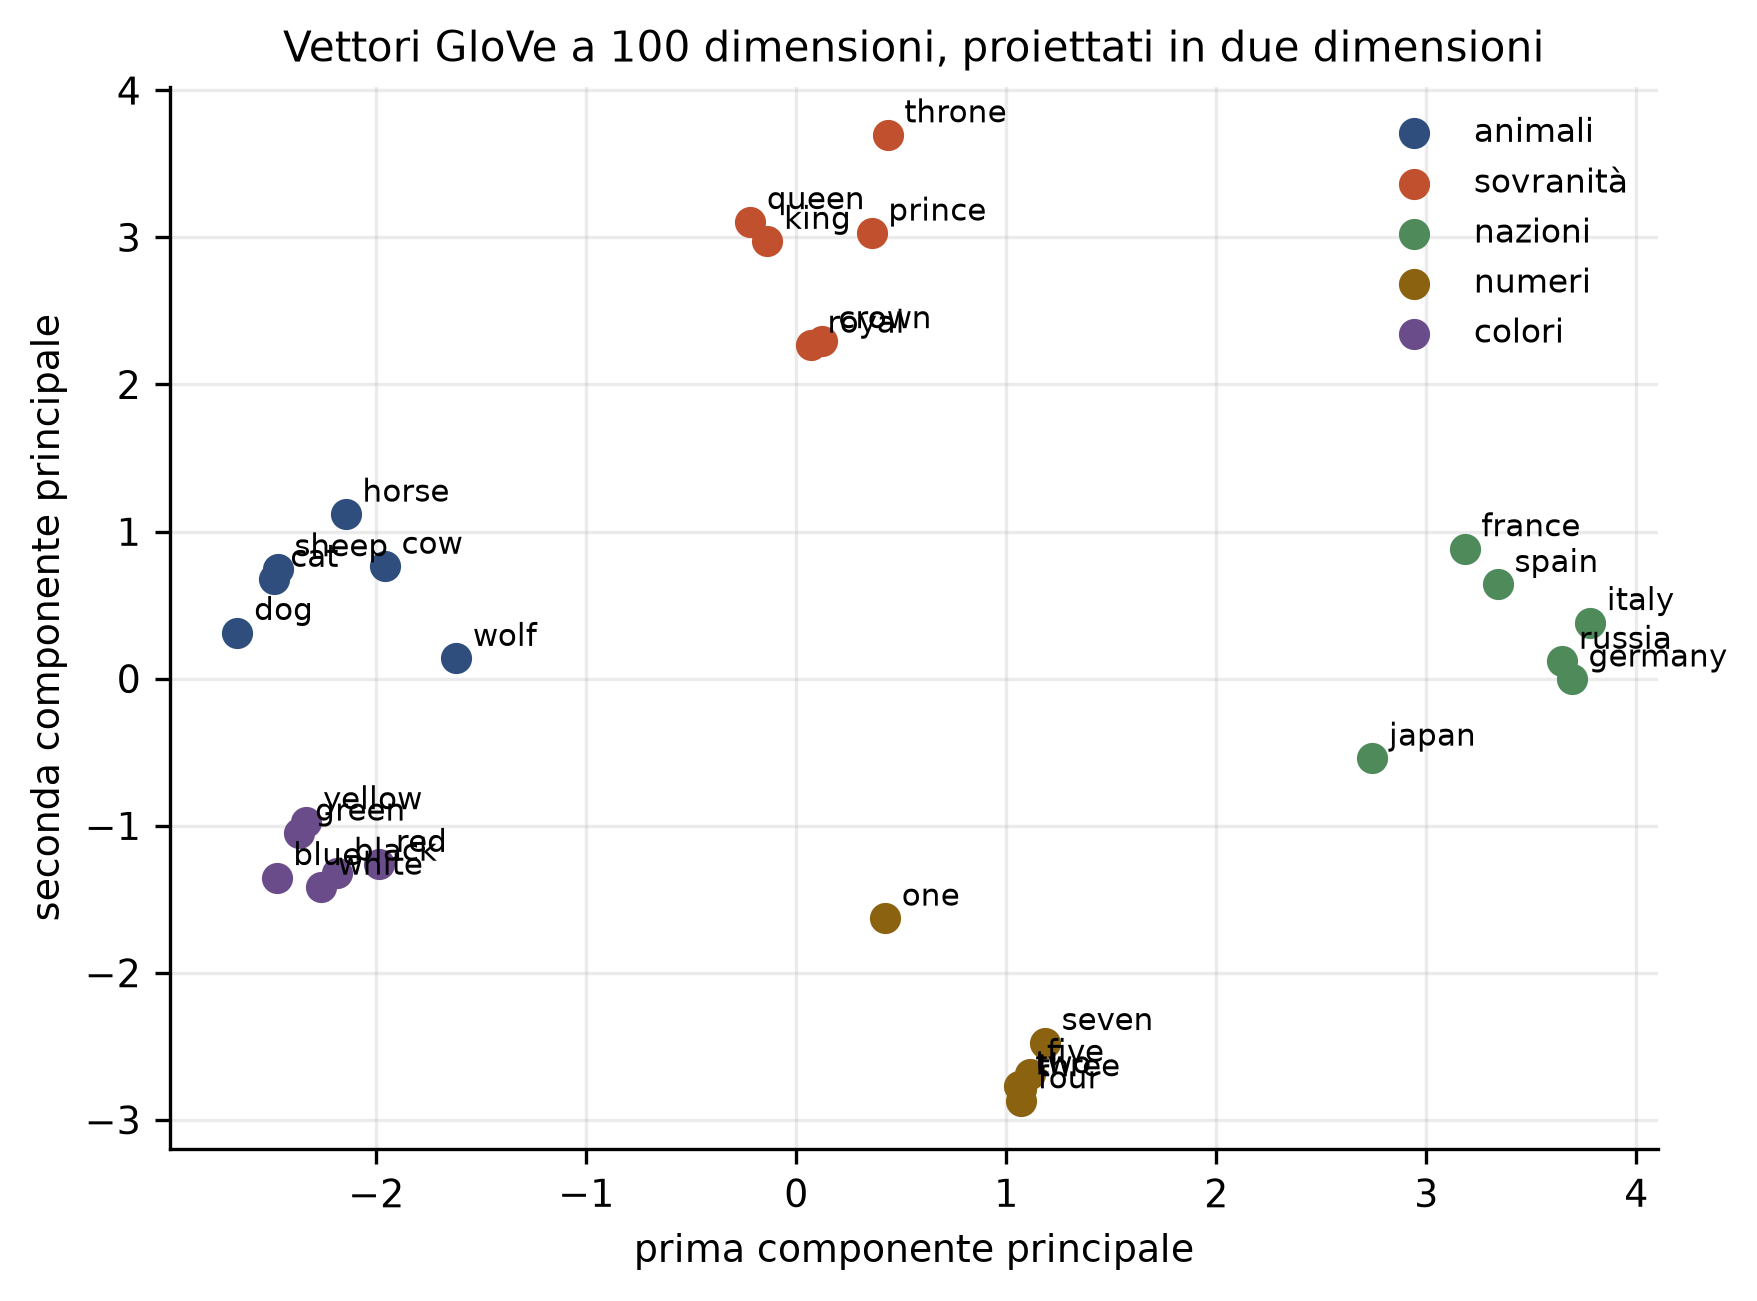
\includegraphics[width=0.82\textwidth]{figure/cap2_embedding_2d.png}
  \caption{Trenta parole inglesi rappresentate dai rispettivi vettori GloVe a
  100 dimensioni, proiettati sulle prime due componenti principali. Le cinque
  famiglie semantiche formano gruppi separati senza che alcuna informazione
  semantica sia stata fornita all'algoritmo. La proiezione conserva soltanto una
  parte della struttura, poiché riduce cento dimensioni a due: la vicinanza
  visibile in figura è una condizione sufficiente, non necessaria, alla
  vicinanza nello spazio originario.}
  \label{fig:embedding}
\end{figure}

I due spazi vettoriali che compaiono in questo lavoro hanno natura diversa. Ogni modello linguistico possiede una propria matrice di embedding,
appresa durante l'addestramento insieme a tutti gli altri parametri, e i cui
vettori non sono direttamente confrontabili fra modelli diversi: fra i modelli
analizzati in questa tesi la dimensione di tale spazio passa da 1536 per il
modello da 1.5 miliardi di parametri a 5120 per quello da 14 miliardi. Gli embedding impiegati nelle analisi di
questa tesi sono invece vettori GloVe a 100 dimensioni, pre-addestrati su un
corpus esterno e identici per tutti i testi esaminati: la scelta è dettata dalla
necessità di misurare i testi generati da modelli diversi con lo stesso metro, e
segue l'impostazione di~\cite{mikhaylovskiy2025states}. Nel
§\ref{sec:traiettoria} tali vettori verranno usati per trasformare un testo in
una traiettoria nello spazio semantico e studiarne l'autocorrelazione.


% ---------------------------------------------------------------------
\section{Generazione autoregressiva e temperatura}
\label{sec:temperatura}

Un modello linguistico autoregressivo, data una sequenza di token $t_{1:m}$,
sceglie il token successivo estraendolo da una distribuzione di probabilità che
dipende dalla sequenza stessa. La probabilità dell'intera sequenza si
decompone per mezzo della regola della catena,
\begin{equation}
  P(t_{1:m}) \;=\; \prod_{k=1}^{m} P(t_k \mid t_{1:k-1}),
  \label{eq:autoregressivo}
\end{equation}
e il modello è addestrato ad approssimare i singoli fattori
$P(t_k \mid t_{1:k-1})$, cioè a prevedere ogni token a partire da tutti quelli
che lo precedono. La generazione consiste nell'applicare ripetutamente questa
previsione, aggiungendo di volta in volta il token estratto alla sequenza che
condiziona l'estrazione successiva.

\paragraph{Origine della distribuzione condizionata.}
Il modo in cui il modello costruisce $P(t_k \mid t_{1:k-1})$ è ciò che
distingue le architetture moderne da quelle precedenti, ed è rilevante per
questo lavoro. I modelli oggi in uso si basano sull'architettura
\emph{transformer}~\cite{vaswani2017}, il cui elemento caratteristico è il
meccanismo di \emph{attenzione}. In esso ogni posizione della sequenza calcola
un peso per ciascuna delle posizioni precedenti e costruisce la propria
rappresentazione come combinazione pesata di quelle: il token in posizione $k$
può quindi attingere direttamente a qualunque token precedente, per lontano che
sia, senza che l'informazione debba propagarsi attraverso le posizioni
intermedie.

È una differenza sostanziale rispetto ai modelli ricorrenti, in cui
l'informazione proveniente da una posizione lontana deve attraversare tutte
quelle interposte e si degrada di conseguenza. Nel transformer il cammino fra
due posizioni qualsiasi ha lunghezza costante, e questo rende l'architettura in
linea di principio capace di rappresentare dipendenze fra porzioni di testo
molto distanti fra loro. È il meccanismo che, negli attuali modelli, potrebbe
dare origine alle correlazioni a lungo raggio descritte nel §\ref{sec:lrc}, e
una delle ragioni per cui ha senso cercarle nel testo generato. La capacità di
rappresentare tali dipendenze non implica però che il modello le riproduca
effettivamente, e l'attenzione opera comunque entro una finestra di contesto
finita: stabilire se le correlazioni siano presenti nel
testo prodotto resta una questione empirica, ed è precisamente quella affrontata
nei capitoli sperimentali.

\paragraph{Temperatura.}
Il modello non produce direttamente probabilità, ma valori reali detti
\emph{logit}, indicati con $u_1,\dots,u_{|\mathcal{L}|}$, uno per ciascun
elemento del dizionario $\mathcal{L}$. Essi vengono convertiti in distribuzione
di probabilità da una funzione softmax riscalata da un parametro
$T$~\cite{ackley1985}:
\begin{equation}
  p(t = \mathcal{L}_l \mid t_{1:i-1}) \;=\;
  \frac{\exp(u_l / T)}{\sum_{l'} \exp(u_{l'} / T)} .
  \label{eq:softmax}
\end{equation}

Il parametro $T$ prende il nome di temperatura, e la denominazione non è una
semplice analogia. Ponendo $E_l = -u_l$, la~\eqref{eq:softmax} coincide con la
distribuzione di Boltzmann $p_l \propto e^{-E_l/T}$ di un sistema a
$|\mathcal{L}|$ stati in equilibrio termico alla temperatura $T$. Questa
identificazione è ciò che giustifica la ricerca, nel testo generato, dei
fenomeni caratteristici dei sistemi termodinamici, e in particolare delle
transizioni di fase discusse nel §\ref{sec:fasi}.

I due limiti sono immediati. Per $T\to0$ la distribuzione si concentra sul token
di logit massimo e la generazione diventa deterministica; per $T\to\infty$ tende
alla distribuzione uniforme sull'intero dizionario, indipendentemente dal
contesto. Fra i due estremi, valori $T<1$ concentrano la massa di probabilità
sugli eventi più probabili, mentre valori $T>1$ la ridistribuiscono verso quelli
meno probabili. La temperatura non modifica dunque ciò che il modello ha
appreso, ma soltanto quanto fedelmente la generazione segue la distribuzione
appresa.

Nella pratica corrente la generazione impiega anche il troncamento della
distribuzione, nelle varianti top-$k$~\cite{fan2018} e
top-$p$~\cite{holtzman2020}, e penalità che scoraggiano la ripetizione. Tutti
questi meccanismi agiscono sulla stessa distribuzione e introducono un secondo
parametro d'ordine, rendendo impossibile attribuire alla sola temperatura il
comportamento osservato. Per questa ragione, e coerentemente con la scelta
esplicita di~\cite{mikhaylovskiy2025zipf}, i dati analizzati in questa tesi sono
stati generati impiegando il solo campionamento per temperatura.


% ---------------------------------------------------------------------
\section{Fasi e stato critico}
\label{sec:fasi}

Una fase di un sistema fisico è uno stato, tipicamente di equilibrio, dotato di
proprietà macroscopiche caratteristiche e stabile in una regione dello spazio
dei parametri; alla frontiera di tali regioni avviene una transizione di fase.
Secondo la classificazione di Ehrenfest~\cite{ehrenfest1933} una transizione di
ordine $n$ è una discontinuità nella derivata $n$-esima dell'energia libera.

Applicare alla lettera questa classificazione al testo generato non è però
possibile. Il sistema considerato non ha un'energia libera di cui prendere
derivate, non è in equilibrio con alcun bagno termico e
non possiede un limite termodinamico, poiché il numero di token di un documento
resta finito. Ciò che rende legittimo il linguaggio delle fasi è la
corrispondenza stabilita nel §\ref{sec:temperatura}: la~\eqref{eq:softmax}
coincide con una distribuzione di Boltzmann in cui i logit giocano il ruolo di
energie e il parametro di campionamento quello di temperatura. La distribuzione
condizionata da cui ogni token viene estratto è dunque, letteralmente, una
distribuzione di Gibbs, e $T$ ne è la temperatura. Quello che resta analogia, e
non identità, è il passaggio dal singolo token al documento: nulla garantisce
che le proprietà collettive di una sequenza generata token per token si
comportino come le proprietà macroscopiche di un sistema all'equilibrio. Il
vocabolario di Ehrenfest viene perciò impiegato in senso descrittivo, per
nominare regioni di comportamento qualitativamente diverso separate da
variazioni rapide, e non per rivendicare una transizione di fase in senso
termodinamico.

Ciò che rende il concetto utile è il comportamento nel punto critico che
separa due fasi: là le correlazioni decadono a legge di potenza e la loro
portata diverge, e molte grandezze osservabili esibiscono lo stesso andamento.
Il criterio inverso, per cui dove compare una legge di potenza si sospetta uno
stato critico, va maneggiato con prudenza, perché distribuzioni a legge di
potenza si generano in molti modi che con la criticità non hanno rapporto, dal
semplice prodotto di variabili aleatorie ai processi di preferential
attachment. Preso da solo, l'andamento a legge di potenza di una quantità non
dimostra nulla. Acquista forza quando più osservabili indipendenti cambiano
regime allo stesso valore del parametro di controllo, ed è in questa forma che
viene impiegato nel §\ref{sec:tstar}: non la legge di potenza di una misura,
ma la convergenza di criteri costruiti per scopi diversi.

Il quadro è stato applicato ai modelli linguistici in~\cite{nakaishi2024}, dove
la temperatura di campionamento separa una fase a bassa temperatura,
caratterizzata da strutture ripetitive, da una ad alta temperatura in cui il
testo è incomprensibile. La tesi sostenuta in quel lavoro è che il linguaggio
naturale si collochi \emph{sul} punto critico fra le due: nello spazio dei
processi stocastici che generano successioni di simboli, il processo
corrispondente a una lingua naturale giacerebbe sulla superficie critica che
separa le due regioni, e un modello addestrato su quella lingua definisce una
famiglia di processi che quella superficie attraversa al variare di $T$. Il
risultato è verificato su modelli da 160 milioni a 2.8 miliardi di parametri, su
sei lingue e su due diverse mappature del testo in successione numerica, il che
ne stabilisce l'indipendenza dalla scala e dalla lingua.

Questa congettura è il punto di contatto più stretto fra il presente lavoro e la
letteratura di fisica statistica sull'argomento, e il
Capitolo~\ref{cap:risultati1} ne fornisce una verifica indipendente: se il
linguaggio naturale è critico, allora la temperatura alla quale il testo
generato somiglia di più a quello umano deve coincidere con quella alla quale il
modello attraversa la transizione, e criteri che misurano proprietà diverse
devono indicarla concordemente.


% ---------------------------------------------------------------------
\subsection{La traiettoria di embedding}
\label{sec:traiettoria}

Il §\ref{sec:token} ha introdotto i vettori di embedding come rappresentazione
del significato. Applicandoli a un testo si ottiene un oggetto geometrico: detta
$(p_1,\dots,p_M)$ la successione delle parole del documento e $v(\cdot)$ la
mappa che associa a una parola il proprio vettore, si pone
\begin{equation}
  \mathbf{m}_i \;=\;
  \begin{cases}
    v(p_i) - \bar{v} & \text{se $p_i$ ha un vettore},\\[2pt]
    \mathbf{0}       & \text{altrimenti},
  \end{cases}
  \label{eq:traiettoria}
\end{equation}
dove $\bar{v}$ è la media dei vettori delle sole parole che ne possiedono uno.
La successione $(\mathbf{m}_1,\dots,\mathbf{m}_M)$ è la traiettoria del testo
nello spazio degli embedding: ogni parola è un punto, e leggere il documento
dall'inizio alla fine equivale a percorrere quella traiettoria.

Due dettagli della~\eqref{eq:traiettoria} incidono sui risultati. Il primo è la
centratura: sottrarre $\bar{v}$ elimina la
direzione media del documento, che altrimenti dominerebbe ogni prodotto scalare
e renderebbe tutte le coppie di parole artificialmente simili. Il secondo è il
trattamento delle parole prive di vettore, alle quali si assegna il vettore
nullo \emph{dopo} la centratura, seguendo~\cite{mikhaylovskiy2025states}: la
posizione nella successione viene così conservata, e con essa la struttura dei
lag, ma la parola non contribuisce ad alcuna correlazione. La conseguenza è che
un testo in cui molte parole non hanno vettore produce una traiettoria fatta in
larga parte di zeri, e le misure che seguono perdono significato prima di
diventare incalcolabili: è la ragione della soglia di validità introdotta più
avanti.

Su questa successione si definisce l'autocorrelazione a distanza $\tau$ come
media della similarità coseno fra i vettori che distano $\tau$ posizioni,
\begin{equation}
  C(\tau) \;=\; \frac{1}{M-\tau} \sum_{i=1}^{M-\tau}
  \frac{\mathbf{m}_i \cdot \mathbf{m}_{i+\tau}}
       {\lVert \mathbf{m}_i \rVert \, \lVert \mathbf{m}_{i+\tau} \rVert},
  \label{eq:acf-embedding}
\end{equation}
con la convenzione che i termini in cui uno dei due vettori è nullo
contribuiscono zero. La~\eqref{eq:acf-embedding} risponde alla domanda: due
parole che distano $\tau$ posizioni tendono a essere semanticamente affini? Vale
$C(\tau) \simeq 0$ quando non c'è alcuna relazione, ed è tanto più vicina a uno
quanto più il testo, a quella distanza, torna a parlare della stessa cosa.

Poiché la~\eqref{eq:acf-embedding} resta calcolabile su qualunque successione,
serve un riferimento che dica quale ampiezza sia distinguibile dal caso. Si
adotta il rimescolamento: si permutano a caso le posizioni della traiettoria, si
ricalcola $C(\tau)$ e si prende il massimo del suo modulo. Il valore così
ottenuto è il livello di rumore del documento, ed è la stessa costruzione dei
null model del §\ref{sec:null}: conserva il contenuto e distrugge l'ordine.
Un'autocorrelazione la cui ampiezza non superi quel livello non è distinguibile
da una successione di parole senza struttura.


% ---------------------------------------------------------------------
\subsection{Le tre fasi}
\label{sec:tre-fasi}

Applicando questo linguaggio al testo generato,
in~\cite{mikhaylovskiy2025states} vengono individuate tre fasi, distinte dal
comportamento di $C(\tau)$.

A bassa temperatura il testo degenera in cicli di ripetizione: la traiettoria
ripassa periodicamente per gli stessi punti, $C(\tau)$ oscilla con periodo pari
alla lunghezza del ciclo e la sua trasformata di Fourier presenta picchi netti.
La quantità che segnala il fenomeno è quindi
\begin{equation}
  \Phi \;=\; \max_{k \ge 1} \bigl\lvert \hat{C}_k \bigr\rvert ,
  \label{eq:periodicita}
\end{equation}
dove $\hat{C}_k$ sono i coefficienti della trasformata discreta di $C(\tau)$. Il
coefficiente $k = 0$ viene escluso perché proporzionale alla media di $C(\tau)$,
cioè al livello complessivo di correlazione e non alla sua periodicità: un testo
uniformemente correlato ma non ciclico ha $\hat{C}_0$ grande e tutti gli altri
coefficienti piccoli. Questa è la fase che, per analogia con gli stati della
materia, viene detta solida. È lo stesso regime in cui, come osservato nel
§\ref{sec:ponte}, la fluttuazione della DFA satura e $\alpha_{\mathrm{DFA}}$
scende verso zero: le due misure segnalano lo stesso fenomeno da due angolazioni
diverse.

La~\eqref{eq:periodicita} si comporta come un parametro d'ordine nel senso che
assume valori grandi in una fase e piccoli nell'altra, ma non si annulla
identicamente fuori dalla fase periodica: su una successione priva di struttura
resta un valore residuo dovuto alle fluttuazioni campionarie. Il
Capitolo~\ref{cap:risultati1} riporta di conseguenza il suo crollo in termini di
ordini di grandezza e non di annullamento.

In una finestra ristretta di temperature $C(\tau)$ decade invece a legge di
potenza: è lo stato critico, quello in cui le leggi di Zipf e di Heaps
introdotte nel §\ref{sec:scala} risultano meglio soddisfatte. Ad alta
temperatura, infine, le correlazioni decadono esponenzialmente e non sussiste
struttura a lungo raggio: è la fase detta amorfa, o gassosa.

Per distinguere le ultime due fasi vengono confrontati due fit
dell'autocorrelazione, uno a legge di potenza e uno esponenziale, tramite il
rapporto dei rispettivi errori~\cite{mikhaylovskiy2023}:
\begin{equation}
  \mathrm{GAPELMAPER} \;=\;
  \frac{\mathrm{MAPE}\bigl(\text{fit a legge di potenza}\bigr)}
       {\mathrm{MAPE}\bigl(\text{fit esponenziale}\bigr)},
  \label{eq:gapelmaper}
\end{equation}
dove il MAPE è quello definito nella~\eqref{eq:mape}. Il rapporto è minore di 1
quando il fit a legge di potenza descrive i dati meglio di quello esponenziale,
e segnala quindi lo stato critico; è maggiore di 1 nella fase amorfa.

La~\eqref{eq:gapelmaper} è un rapporto fra errori di fit, e come tale resta
calcolabile anche quando l'autocorrelazione è indistinguibile dal rumore; in
quel regime, però, il suo valore è privo di contenuto informativo, perché
entrambi i fit descrivono male dati che non contengono alcun segnale.

Le tre fasi, la soglia di periodicità e la condizione di validità si compongono
nella regola seguente. Detti $\kappa$ la quota di parole del documento dotate di
un vettore, $A = \max_\tau \lvert C(\tau)\rvert$ l'ampiezza
dell'autocorrelazione e $\eta$ il livello di rumore stimato per rimescolamento,
un documento viene classificato come
%
\begin{itemize}
  \item \emph{non valutabile}, se $\kappa < \kappa_{\min}$ oppure $A \le \eta$;
  \item \emph{solido}, altrimenti, se $\Phi > \Phi_{\min}$;
  \item \emph{critico}, altrimenti, se $\mathrm{GAPELMAPER} < 1$;
  \item \emph{amorfo} in ogni altro caso.
\end{itemize}
%
L'ordine dei controlli non è indifferente. La condizione di validità viene per
prima perché le altre due misure, su un documento che non la supera, sono numeri
senza referente; la periodicità viene prima del GAPELMAPER perché
un'autocorrelazione periodica non è né una legge di potenza né un esponenziale,
e sottoporla a quel confronto restituirebbe un valore arbitrario. I due valori
di soglia sono fissati nel Capitolo~\ref{cap:risultati1}, dove ne vengono
discussi l'origine e l'effetto.

I due quadri di riferimento non coincidono del tutto.
In~\cite{nakaishi2024} le fasi sono due e ciò che le separa è un punto critico,
cioè un insieme di misura nulla nello spazio dei parametri;
in~\cite{mikhaylovskiy2025states} lo stato critico diventa invece una fase a sé,
dotata di estensione finita. La differenza non è terminologica: nel primo caso
attraversare la transizione con uno sweep a passo finito significa quasi
certamente saltare il punto critico, nel secondo significa attraversare una
regione che si può campionare. Il Capitolo~\ref{cap:risultati1} riporta i dati
pertinenti alla questione senza pretendere di risolverla.


% ---------------------------------------------------------------------
\section{Notazione}
\label{sec:notazione}

Le grandezze introdotte in questo capitolo provengono da lavori che adottano
simboli in conflitto fra loro. La Tabella~\ref{tab:notazione} raccoglie la
notazione seguita in questa tesi, che viene mantenuta senza eccezioni nei
capitoli successivi.

\begin{table}[htbp]
\centering
\small
\begin{tabular}{@{}l>{\raggedright\arraybackslash}p{8.3cm}c@{}}
\toprule
Simbolo & Grandezza & Definita in \\
\midrule
\multicolumn{3}{@{}l}{\itshape Testo e vocabolario} \\
$\mathbf{W}$, $w_t$, $N$ & sequenza di parole, parola in posizione $t$, lunghezza & \eqref{eq:sequenza} \\
$\mathcal{D}$, $\mathcal{D}(t)$ & dizionario e dizionario parziale & §\ref{sec:scala} \\
$f(r)$, $\alpha$ & frequenza della parola di rango $r$, esponente di Zipf & \eqref{eq:zipf} \\
$\gamma_H$ & esponente di Heaps & \eqref{eq:heaps} \\
$R$ & parole nuove nella seconda metà, rapportate alla prima & \eqref{eq:R} \\
MAPE & errore percentuale assoluto medio del fit & \eqref{eq:mape} \\
\addlinespace
\multicolumn{3}{@{}l}{\itshape Correlazioni} \\
$x_k$ & successione binaria generata da un osservabile & \eqref{eq:osservabile} \\
$c(s)$, $\theta$ & autocorrelazione a distanza $s$ e suo esponente di decadimento & \eqref{eq:acf-power} \\
$X(t)$, $\sigma_X^2$, $\gamma$ & conteggio, sua varianza, esponente di crescita & \eqref{eq:sigma} \\
$F(s)$, $\alpha_{\mathrm{DFA}}$ & fluttuazione detrendizzata e suo esponente & \eqref{eq:dfa-alpha} \\
\addlinespace
\multicolumn{3}{@{}l}{\itshape Intervalli e burstiness} \\
$\tau_i$, $p(\tau)$ & intervalli fra occorrenze e loro distribuzione & §\ref{sec:burst} \\
cv, $B$ & coefficiente di variazione, indice di Goh--Barabási & \eqref{eq:cv}, \eqref{eq:goh} \\
$S(0)$, $c_\tau(k)$ & spettro a frequenza nulla, autocorrelazione degli intervalli & \eqref{eq:eq4} \\
$\hat\gamma_{A1}$, $\hat\gamma_{A2}$ & esponenti misurati sui due null model & §\ref{sec:null} \\
$q$ & quota di burstiness & \eqref{eq:quota} \\
$\mu$, $\tau_c$ & esponente di coda e cut-off di $p(\tau)$ & \eqref{eq:troncata} \\
$J$ & entropia degli intervalli, riferita al processo di Poisson & \eqref{eq:entropia-intervalli} \\
\addlinespace
\multicolumn{3}{@{}l}{\itshape Entropia e compressione} \\
$H$, $h$ & entropia di Shannon, tasso di entropia & \eqref{eq:H-singola}, \eqref{eq:tasso-entropia} \\
$c(x|y)$, $h(x|y)$ & frasi del cross-parsing, cross-entropia stimata & \eqref{eq:crossparsing} \\
$D(x\|y)$, $D_s$ & divergenza di Kullback--Leibler e sua versione simmetrizzata & \eqref{eq:kl}, \eqref{eq:kl-sym} \\
$C(x)$, $R_{\mathrm{gzip}}$ & dimensione compressa e rapporto di compressione & \eqref{eq:cratio} \\
NCD & distanza normalizzata di compressione & \eqref{eq:ncd} \\
\addlinespace
\multicolumn{3}{@{}l}{\itshape Generazione e fasi} \\
$u_l$, $T$ & logit del token $l$, temperatura di campionamento & \eqref{eq:softmax} \\
$C(\tau)$ & autocorrelazione della traiettoria di embedding & \eqref{eq:acf-embedding} \\
$\Phi$ & parametro di periodicità di $C(\tau)$ & \eqref{eq:periodicita} \\
GAPELMAPER & rapporto fra gli errori dei due fit dell'autocorrelazione & \eqref{eq:gapelmaper} \\
$N_{\mathrm{eff}}$ & lunghezza comune di analisi & §\ref{sec:scelte} \\
\bottomrule
\end{tabular}
\caption{Notazione adottata in questa tesi.}
\label{tab:notazione}
\end{table}

Per tre simboli la scelta operata qui si discosta da quella di almeno una delle
fonti; la Tabella~\ref{tab:collisioni} riassume le corrispondenze.

\begin{center}
\small
\begin{tabular}{@{}lcccc@{}}
\toprule
Grandezza & Qui & \cite{mikhaylovskiy2025zipf} & \cite{lippi2019} & \cite{altmann2012} \\
\midrule
Esponente di Zipf                  & $\alpha$                & $\alpha$ & $\beta$  & --- \\
Esponente di Heaps                 & $\gamma_H$              & $\beta$  & $\nu$    & --- \\
Esponente della fluttuazione (DFA) & $\alpha_{\mathrm{DFA}}$ & ---      & $\alpha$ & --- \\
Decadimento dell'autocorrelazione  & $\theta$                & ---      & $\gamma$ & $\beta$ \\
Crescita della varianza del conteggio & $\gamma$             & ---      & ---      & $\gamma$ \\
Rapporto di compressione           & $R_{\mathrm{gzip}}$     & ---      & ---      & --- \\
\bottomrule
\end{tabular}
\captionof{table}{Corrispondenza fra la notazione adottata e quella delle fonti primarie,
limitatamente ai simboli per cui le fonti divergono. Il rapporto di compressione
è indicato con $R(x)$ in~\cite{hadad2026}, dove però $R$ non ha il significato
che assume qui.}
\label{tab:collisioni}
\end{center}

Il simbolo $\alpha$ è riservato all'esponente di Zipf, come
in~\cite{mikhaylovskiy2025zipf}, mentre l'esponente della detrended
fluctuation analysis, indicato con $\alpha$ in~\cite{lippi2019}, riceve il
pedice $\mathrm{DFA}$. L'esponente di Heaps è indicato con $\gamma_H$ anziché
con $\beta$ o $\nu$, per lasciare $\gamma$ libero per l'esponente di crescita
della varianza del conteggio, che è la convenzione di~\cite{altmann2012} e
della seconda parte sperimentale. Il decadimento dell'autocorrelazione riceve
infine il simbolo $\theta$, che nessuna delle fonti impiega, poiché entrambe
le lettere che gli sono attribuite in letteratura sono già assegnate. La
lettera $R$ resta al descrittore di~\cite{mikhaylovskiy2025zipf} e il rapporto
di compressione riceve il pedice $\mathrm{gzip}$.

Valgono inoltre le convenzioni seguenti, usate nel seguito senza ulteriore
avviso. Il circonflesso indica una quantità stimata dai dati in contrapposizione
al corrispondente valore teorico, come in $\hat\gamma$. I pedici $A1$ e $A2$
indicano i due null model del §\ref{sec:null}. Il simbolo $|\cdot|$ applicato a
un insieme ne indica la cardinalità e applicato a un testo la lunghezza, in
parole o in byte secondo il contesto. Le medie sono indicate con
$\langle\cdot\rangle$ e si intendono calcolate sull'intero documento salvo
diversa indicazione.

%  Le figure sono attese in figure/; la provenienza e in appendice_figure.tex
% =====================================================================

\chapter{Quadro teorico}
\label{cap:teoria}

In questo capitolo si introducono gli strumenti matematici con cui storicamente
si sono analizzati i testi e che, anche in questo lavoro, ricopriranno un ruolo
centrale: le leggi di scala del vocabolario, le misure di correlazione a lungo
raggio, la statistica degli intervalli fra occorrenze e le stime di entropia
ottenute per compressione.

Successivamente vengono introdotti gli elementi di base del funzionamento dei
modelli linguistici di grandi dimensioni, il linguaggio delle transizioni di
fase con cui alcuni risultati verranno interpretati, e la notazione adottata nel
resto della tesi.


% ---------------------------------------------------------------------
\section{Leggi di scala del vocabolario}
\label{sec:scala}

Come già anticipato, un testo può essere visto come una sequenza di simboli,
siano essi lettere, parole o, come si vedrà nel §\ref{sec:token}, token. La
scelta più naturale per un lettore umano è assumere come unità fondamentale la
parola, in quanto più piccola unità di testo dotata di significato autonomo.

Un testo è quindi una sequenza ordinata di parole
\begin{equation}
  \mathbf{W} \;=\; (w_1, w_2, \dots, w_N),
  \label{eq:sequenza}
\end{equation}
dove $N$ è la lunghezza del testo e l'indice $t = 1,\dots,N$ individua la
posizione di ciascuna parola. L'insieme delle parole distinte che vi compaiono
si dice dizionario e si indica con $\mathcal{D}$; si definisce inoltre il
dizionario parziale $\mathcal{D}(t)$ come l'insieme delle parole distinte
contenute nel prefisso $(w_1,\dots,w_t)$. Valgono per costruzione
$\mathcal{D}(N) = \mathcal{D}$ e $\mathcal{D}(t) \subseteq \mathcal{D}(t+1)$: il
dizionario parziale è una successione non decrescente di insiemi.

A titolo di esempio si consideri la frase
\begin{center}
\emph{Se pensi di comprendere la meccanica quantistica, non comprendi la
meccanica quantistica.}
\end{center}
Con la notazione introdotta si ha $N = 12$, $w_7 = \text{\emph{quantistica}}$ e
\begin{align}
  \mathcal{D}    &= \{\text{se, pensi, di, comprendere, la, meccanica,
                          quantistica, non, comprendi}\}, \\
  \mathcal{D}(6) &= \{\text{se, pensi, di, comprendere, la, meccanica}\} .
\end{align}
Il dizionario completo contiene nove parole distinte a fronte di dodici
occorrenze: le tre ripetizioni di \emph{la}, \emph{meccanica} e
\emph{quantistica} non lo accrescono.

Le due analisi più semplici che si possano condurre su $\mathbf{W}$ sono lo
studio delle frequenze delle singole parole e quello dell'andamento di
$|\mathcal{D}(t)|$ in funzione di $t$. Sono le analisi che hanno portato alla
formulazione delle due leggi empiriche enunciate nel seguito, dovute
rispettivamente a Zipf~\cite{zipf1949} e a Herdan~\cite{herdan1964} e
Heaps~\cite{heaps1978}.

% ---------------------------------------------------------------------
\subsection{Legge di Zipf}
\label{sec:zipf}

Si contino le occorrenze di ciascuna parola distinta e si ordinino le parole per
frequenza decrescente, associando a ognuna il proprio rango $r$: la parola di
rango 1 è la più frequente del testo, quella di rango 2 la seconda, e così via.
Detta $f(r)$ la frequenza della parola di rango $r$, si osserva empiricamente in
tutti i testi naturali che
\begin{equation}
  f(r) \;\propto\; r^{-\alpha}.
  \label{eq:zipf}
\end{equation}
La~\eqref{eq:zipf} prende il nome di legge di Zipf. In coordinate
bilogaritmiche corrisponde a una retta di pendenza $-\alpha$, ed è in tali
coordinate che viene di norma rappresentata e stimata.

La Figura~\ref{fig:zipf} riporta la relazione rango-frequenza per cinque romanzi
in cinque lingue diverse. Le curve sono approssimativamente rettilinee su circa
tre decadi di rango e hanno pendenze molto simili fra loro, nonostante le opere
differiscano per epoca, lingua e lunghezza.

\begin{figure}[htbp]
  \centering
  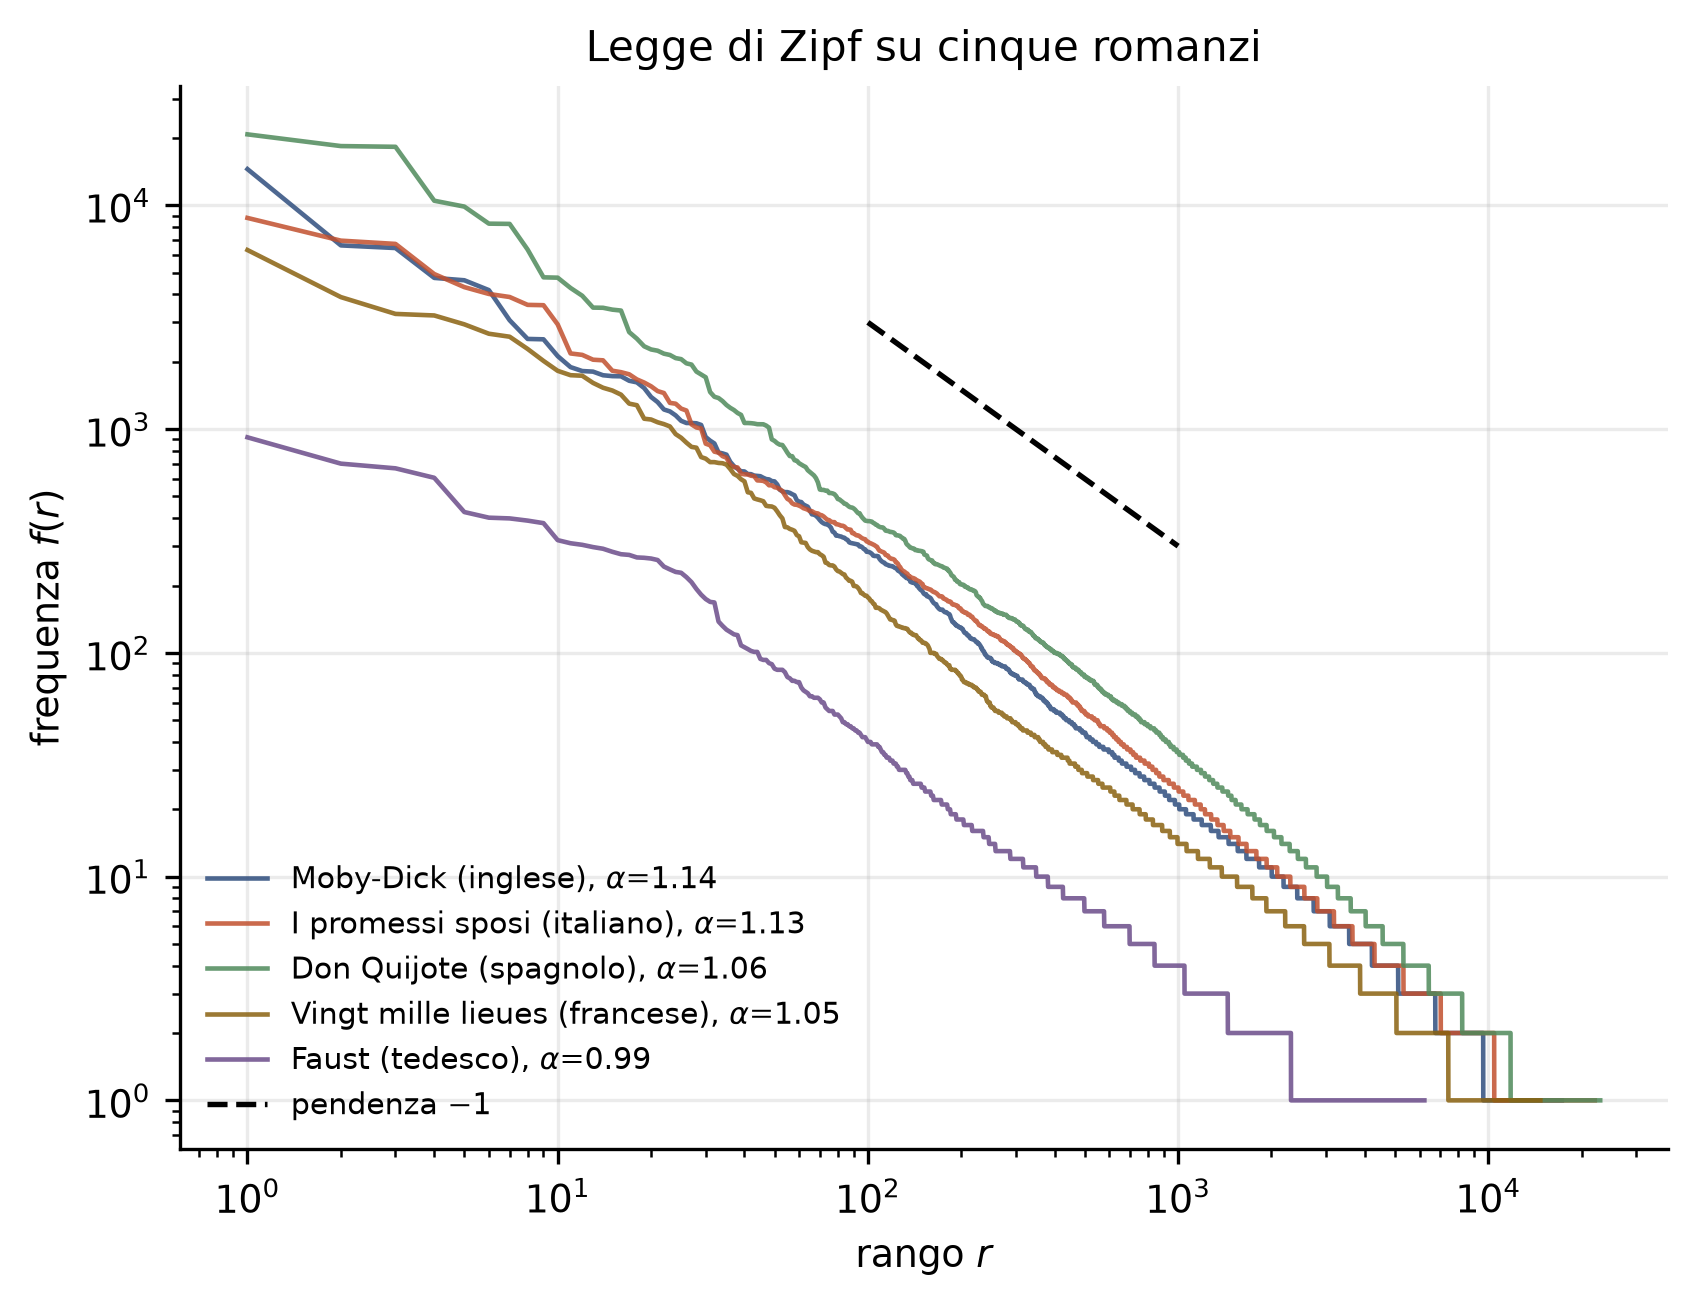
\includegraphics[width=0.82\textwidth]{figure/cap2_zipf_lingue.png}
  \caption{Relazione rango-frequenza per cinque romanzi in altrettante lingue,
  in coordinate bilogaritmiche. Gli esponenti riportati in legenda sono stimati
  per regressione ai minimi quadrati nella finestra di ranghi
  $10^2 \le r \le 10^3$, la stessa impiegata in~\cite{lippi2019}. La retta
  tratteggiata ha pendenza $-1$ ed è riportata come riferimento visivo.}
  \label{fig:zipf}
\end{figure}

Il parametro $\alpha$ risulta positivo e prossimo a 1 nella grande maggioranza
delle lingue esaminate, comprese quelle estinte e quelle costruite
artificialmente. Valori di
$\alpha$ più alti sono sintomo di un vocabolario più povero, poiché un numero
minore di parole esaurisce la maggior parte del testo; valori più bassi
segnalano al contrario una presenza più marcata di parole rare.

I valori misurati sulle cinque opere della Figura~\ref{fig:zipf} sono raccolti
nella Tabella~\ref{tab:zipf-misure}, accanto ai valori medi per lingua riportati
in~\cite{mikhaylovskiy2025zipf} su un corpus di sei opere letterarie in cinque
lingue.

\begin{table}[htbp]
\centering
\small
\begin{tabular}{@{}llrrr@{}}
\toprule
Opera & Lingua & Parole & $|\mathcal{D}|$ & $\alpha$ \\
\midrule
Moby-Dick               & inglese   & \num{219081} & \num{17258} & 1.14 \\
I promessi sposi        & italiano  & \num{239353} & \num{22040} & 1.13 \\
Don Quijote             & spagnolo  & \num{383633} & \num{22943} & 1.06 \\
Vingt mille lieues sous les mers & francese & \num{148923} & \num{14716} & 1.05 \\
Faust                   & tedesco   & \num{30959}  & \num{6221}  & 0.99 \\
\bottomrule
\end{tabular}
\caption{Esponente di Zipf misurato sulle cinque opere della
Figura~\ref{fig:zipf}, con il numero di occorrenze e la dimensione del
dizionario. La stima è condotta sui ranghi $10^2$--$10^3$.}
\label{tab:zipf-misure}
\end{table}

\begin{table}[htbp]
\centering
\small
\begin{tabular}{@{}lcccc@{}}
\toprule
& \multicolumn{2}{c}{$\alpha$ (Zipf)} & \multicolumn{2}{c}{$\gamma_H$ (Heaps)} \\
\cmidrule(lr){2-3}\cmidrule(lr){4-5}
Lingua & parole & token & parole & token \\
\midrule
inglese  & $0.952 \pm 0.072$ & $0.985 \pm 0.054$ & $0.809 \pm 0.027$ & $0.802 \pm 0.024$ \\
tedesco  & $0.959 \pm 0.054$ & $1.024 \pm 0.042$ & $0.846 \pm 0.031$ & $0.793 \pm 0.028$ \\
russo    & $1.043 \pm 0.077$ & $1.009 \pm 0.067$ & $0.916 \pm 0.049$ & $0.805 \pm 0.025$ \\
spagnolo & $0.962 \pm 0.030$ & $1.016 \pm 0.035$ & $0.842 \pm 0.025$ & $0.798 \pm 0.028$ \\
francese & $0.963 \pm 0.033$ & $0.989 \pm 0.042$ & $0.843 \pm 0.020$ & $0.801 \pm 0.018$ \\
\bottomrule
\end{tabular}
\caption{Esponenti medi per lingua riportati in~\cite{mikhaylovskiy2025zipf},
misurati su sei opere letterarie per ciascuna lingua, a livello di parola e di
token. In quel lavoro $\alpha$ è stimato sulla rappresentazione
cumulata della distribuzione anziché sulla relazione rango-frequenza; i due
stimatori coincidono soltanto nel limite $\alpha \to 1$, e i valori non vanno
quindi confrontati direttamente con quelli della
Tabella~\ref{tab:zipf-misure}.}
\label{tab:zipf-letteratura}
\end{table}

Sui testi reali si osservano deviazioni sistematiche dalla~\eqref{eq:zipf}. Su
corpora molto ampi l'esponente resta prossimo a 1 soltanto per le prime migliaia
di parole, mentre la coda continua a seguire una legge di potenza ma con
esponente maggiore~\cite{piantadosi2014}. Le parole più frequenti, inoltre,
mostrano frequenze leggermente inferiori a quelle previste: una deviazione che
Mandelbrot~\cite{mandelbrot1953} corregge introducendo un termine additivo nel
rango,
\begin{equation}
  f(r) \;\propto\; (r + c)^{-\alpha},
  \label{eq:mandelbrot}
\end{equation}
dove la costante $c > 0$ attenua la divergenza della legge di potenza ai ranghi
più bassi, spostando di fatto l'origine dell'asse dei ranghi e rendendo il fit
aderente anche nella regione delle parole più comuni.

\paragraph{Bontà del fit.}
Come si vedrà nei capitoli sperimentali, sui testi generati automaticamente
l'aderenza alla legge di potenza non è garantita. Il solo esponente non è
sufficiente a stabilirla, perché descrive la pendenza media della curva e non la
sua forma: una curva marcatamente incurvata in coordinate bilogaritmiche può
avere la stessa pendenza media di una retta, e restituire quindi un valore di
$\alpha$ del tutto ordinario pur non essendo una legge di potenza. Occorre
perciò una seconda quantità, che misuri quanto i dati si discostino dalla retta
interpolante.

Seguendo~\cite{mikhaylovskiy2025zipf}, la qualità del fit viene stimata con
l'errore percentuale assoluto medio
\begin{equation}
  \mathrm{MAPE} \;=\; \frac{1}{n}\sum_{i=1}^{n}
  \left| \frac{y_i - \hat{y}_i}{y_i} \right|,
  \label{eq:mape}
\end{equation}
dove $n$ è il numero di punti su cui è condotta la regressione, $y_i$ il valore
osservato e $\hat{y}_i$ quello previsto dalla retta interpolante in
corrispondenza dello stesso rango. Il MAPE è nullo per dati perfettamente
allineati e cresce al crescere della distanza relativa dalla retta;
essendo definito su scarti relativi, non dipende dall'unità di misura né
dall'ampiezza delle frequenze, e resta quindi confrontabile fra testi di
lunghezza diversa.

Sul corpus di testi letterari usato in~\cite{mikhaylovskiy2025zipf} il MAPE vale
in media $0.156$ con deviazione standard $0.077$. Nei capitoli sperimentali il
suo minimo in funzione della temperatura di generazione individuerà il regime in
cui il testo prodotto è più vicino a una legge di potenza.

% ---------------------------------------------------------------------
\subsection{Legge di Heaps}
\label{sec:heaps}

Studiando l'andamento di $|\mathcal{D}(t)|$ nei testi letterari emerge una
seconda regolarità, nota come legge di Heaps o, dal nome di chi la formulò per
primo~\cite{herdan1964}, di Herdan--Heaps:
\begin{equation}
  |\mathcal{D}(t)| \;\propto\; t^{\gamma_H}, \qquad \gamma_H \in [0,1] .
  \label{eq:heaps}
\end{equation}
Qui $t$ è la posizione nel testo, misurata in numero di parole,
$|\mathcal{D}(t)|$ la dimensione del dizionario parziale e $\gamma_H$
l'esponente di Heaps. I due estremi dell'intervallo corrispondono a due
comportamenti limite: $\gamma_H = 0$ descrive un dizionario che cessa di
crescere, cioè un testo che non introduce più parole nuove, mentre
$\gamma_H = 1$ descrive un dizionario che cresce proporzionalmente alla
lunghezza, cioè un testo in cui ogni parola è nuova. Poiché il dizionario non
può crescere più rapidamente del testo che lo contiene, si ha necessariamente
$|\mathcal{D}(t)| \le t$, e l'esponente non può eccedere l'unità.

La legge di Heaps quantifica dunque la capacità di un testo di rinnovare il
proprio vocabolario, ed è per questo particolarmente istruttiva se si torna alla
Tabella~\ref{tab:tre-regimi} del Capitolo~\ref{cap:introduzione}. Il primo
esempio, monotono e ripetitivo, cessa rapidamente di accrescere il dizionario;
l'ultimo, in cui i caratteri sono estratti a caso, produce quasi soltanto parole
nuove e fa crescere il dizionario senza saturare. La Figura~\ref{fig:heaps}
mostra le curve dei due casi limite accanto a quelle di tre testi letterari.

\begin{figure}[htbp]
  \centering
  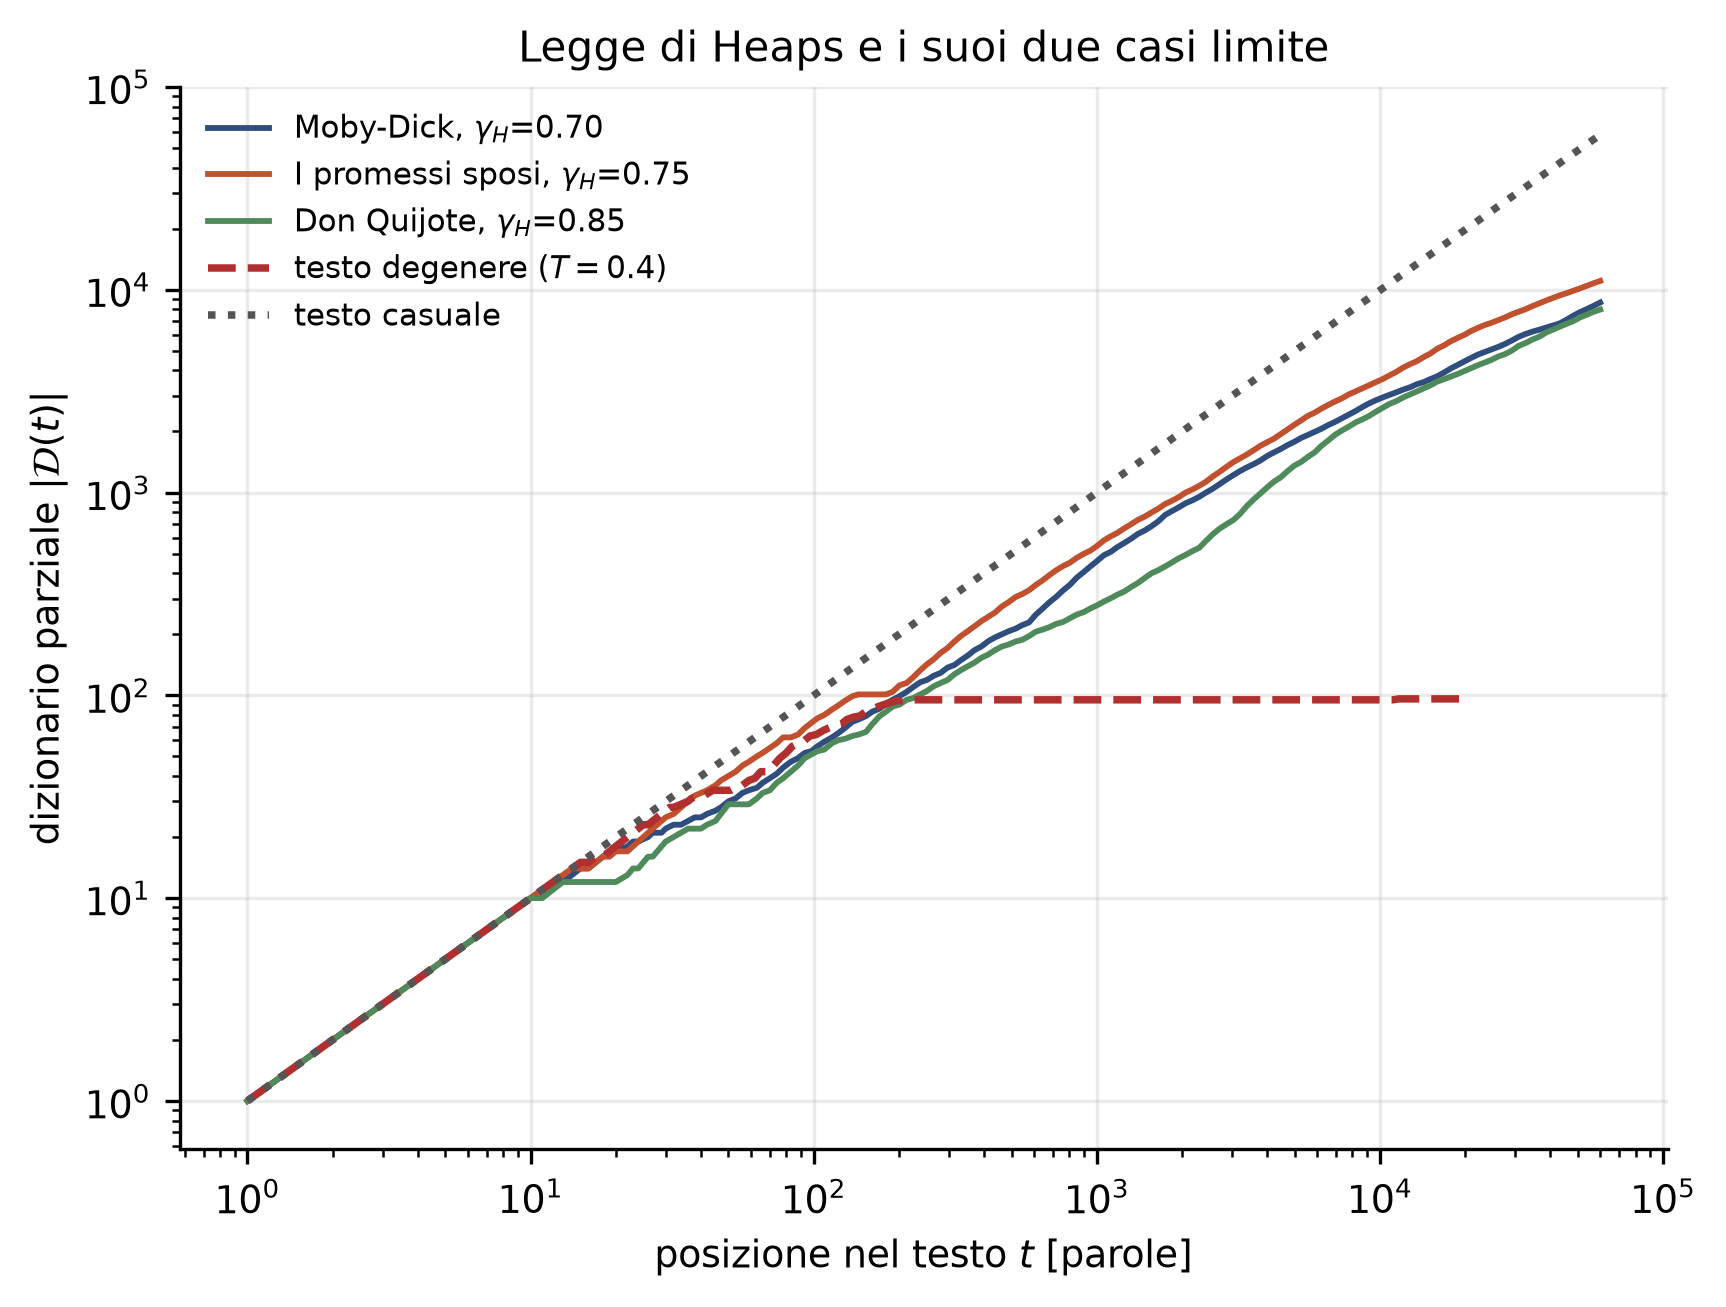
\includegraphics[width=0.82\textwidth]{figure/cap2_heaps_confronto.png}
  \caption{Crescita del dizionario parziale in coordinate bilogaritmiche. Le tre
  curve continue sono testi letterari, con esponente stimato nella regione
  $t > 1000$. La curva tratteggiata è il campione generato a $T = 0.4$ già
  riportato nella Tabella~\ref{tab:tre-regimi}: dopo circa un centinaio di
  parole entra in un ciclo di ripetizione e il dizionario si arresta. La curva
  punteggiata è una sequenza di caratteri casuali, in cui ogni parola è nuova e
  la crescita è esattamente lineare.}
  \label{fig:heaps}
\end{figure}

L'esponente stimato dipende inoltre dall'intervallo su cui viene condotta la
regressione, e quindi dalla lunghezza del testo analizzato. La
Figura~\ref{fig:heaps-finito} mostra l'effetto su tre opere: ripetendo la stima
su prefissi via via più lunghi della stessa opera, $\gamma_H$ decresce in modo
sistematico, di oltre un decimo fra $10^4$ e $10^5$ parole. Il fenomeno è la
prima manifestazione degli effetti di dimensione finita discussi in modo
generale nel §\ref{sec:lunghezza}, ed è già segnalato
in~\cite{mikhaylovskiy2025zipf}, dove si osserva che per $\alpha$ prossimo a 1
la crescita del dizionario è descritta meglio dalla forma $t/\ln t$ che da una
pura legge di potenza. Ai valori di $N$ più bassi la regressione si appoggia a
un intervallo troppo corto e può restituire stime superiori a 1, incompatibili
con il limite teorico: è un artefatto della finestra di fit, non una proprietà
del testo.

\begin{figure}[htbp]
  \centering
  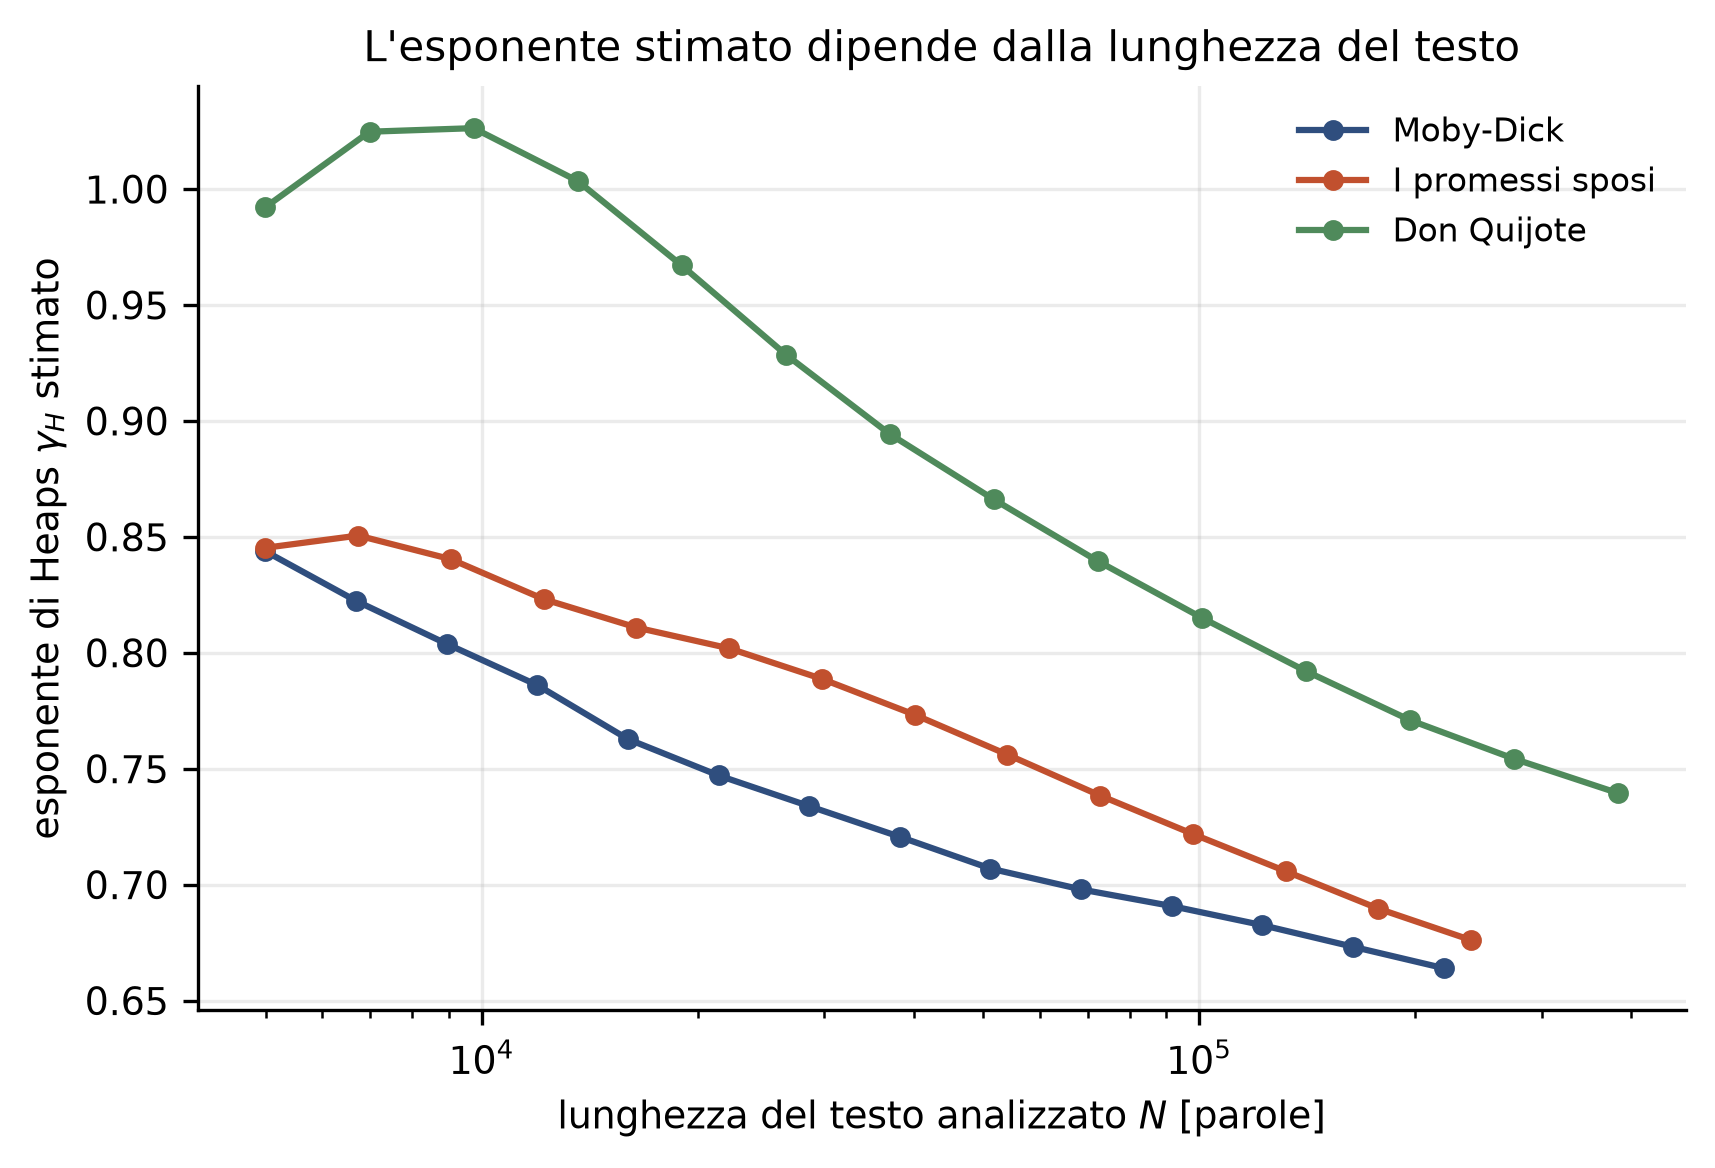
\includegraphics[width=0.78\textwidth]{figure/cap2_heaps_dimensione_finita.png}
  \caption{Esponente di Heaps stimato su prefissi di lunghezza crescente, per tre
  opere in tre lingue diverse, con regressione condotta nella regione $t > 1000$.
  La deriva è sistematica e comune a tutte e tre, ed è quindi una proprietà dello
  stimatore e non di una particolare opera: confrontare esponenti misurati su
  testi di lunghezza diversa non è lecito. Il §\ref{sec:scelte} riprende
  l'effetto su una sola opera, misurandone però l'entità su tutti gli stimatori
  impiegati in questa tesi.}
  \label{fig:heaps-finito}
\end{figure}

\paragraph{Il descrittore $R$.}
Sui testi generati automaticamente la difficoltà è più radicale. A bassa
temperatura di generazione il modello entra in un ciclo di ripetizione e cessa
di produrre parole nuove: la curva $|\mathcal{D}(t)|$ diventa piatta e
la~\eqref{eq:heaps} perde significato. Ad alta temperatura si verifica il caso
opposto, con quasi ogni parola nuova e curva prossima alla linearità. In
entrambe le situazioni la stima di $\gamma_H$ restituisce un numero privo di
contenuto, come mostrano le due curve estreme della Figura~\ref{fig:heaps}.

Per questa ragione in~\cite{mikhaylovskiy2025zipf} viene introdotto un
descrittore che resta definito in ogni regime. Detti $\mathcal{D}_1$ il
dizionario della prima metà del testo e $\mathcal{D}_2$ quello della seconda, si
pone
\begin{equation}
  R \;=\; \frac{|\mathcal{D}_2 \setminus \mathcal{D}_1|}{|\mathcal{D}_1|},
  \label{eq:R}
\end{equation}
cioè il rapporto fra il numero di parole che compaiono per la prima volta nella
seconda metà del testo e il numero di quelle che compaiono per la prima volta
nella prima. Un testo degenerato ha $R$ prossimo a zero, poiché la seconda metà
non introduce nulla di nuovo; un testo in cui ogni parola è nuova ha $R$
prossimo a uno. Sul corpus di opere letterarie intere usato
in~\cite{mikhaylovskiy2025zipf} il valore medio è $R = 0.17$ con deviazione
standard $0.05$.


% ---------------------------------------------------------------------
\section{Correlazioni a lungo raggio}
\label{sec:lrc}

Sia la legge di Zipf sia quella di Heaps ignorano l'ordine dei simboli. Per la
prima l'affermazione è immediata: la~\eqref{eq:zipf} dipende soltanto dai
conteggi delle parole, e un rimescolamento del testo li lascia invariati. Per la
seconda l'invarianza è meno diretta: rimescolando il testo la curva
$|\mathcal{D}(t)|$ cambia realizzazione, perché cambia l'ordine in cui le
parole compaiono per la prima volta, ma il suo andamento medio resta lo stesso, e con esso l'esponente
$\gamma_H$. Entrambe sono quindi proprietà del vocabolario, non della sequenza.

Per misurare le proprietà che dipendono dall'ordine occorre estrarre dal testo
un segnale, cioè una successione finita di valori reali, e studiarne le
correlazioni a scale diverse. La costruzione del segnale non è unica, e ogni
scelta mette in luce aspetti differenti: si può codificare la posizione delle
singole lettere o di classi di lettere, quella delle parole o di classi
grammaticali, oppure la lunghezza delle frasi. In tutti i casi si osserva che il
linguaggio esibisce correlazioni a lungo raggio, con una struttura che si
estende su molti ordini di grandezza~\cite{altmann2012,montemurro2002}.

% ---------------------------------------------------------------------
\subsection{Funzione di autocorrelazione}
\label{sec:acf}

Data una successione $x_1,\dots,x_N$, la funzione di autocorrelazione a distanza
$s$ è
\begin{equation}
  c(s) \;=\; \langle x_n x_{n+s}\rangle
  - \langle x_n\rangle\langle x_{n+s}\rangle ,
  \label{eq:acf}
\end{equation}
dove $\langle\cdot\rangle$ indica la media su tutte le posizioni $n$ compatibili
con la distanza $s$. La forma funzionale di $c(s)$ distingue i regimi di
correlazione.

Se i valori non sono correlati, $c(s)$ è identicamente nulla per $s \neq 0$. Se
$c(s)$ decade esponenzialmente,
$c(s) \sim e^{-s/s_0}$, il segnale si dice correlato a corto raggio: la costante
$s_0$ ha le dimensioni di una distanza e ne fissa la scala caratteristica, nel
senso che oltre poche volte $s_0$ la correlazione è numericamente
indistinguibile da zero. Esiste dunque una distanza tipica oltre la quale due
porzioni di segnale sono indipendenti, e il sistema non possiede struttura al di
là di essa.

Si dice invece che il segnale è correlato a lungo raggio quando il decadimento
segue la legge di potenza
\begin{equation}
  c(s) \;\sim\; s^{-\theta},
  \label{eq:acf-power}
\end{equation}
con $0<\theta<1$. In questo caso non esiste alcuna scala privilegiata: la
funzione~\eqref{eq:acf-power} è invariante di scala, cioè riscalare $s$ di un
fattore costante riscala $c$ di un fattore costante senza modificarne la forma,
e un certo grado di correlazione persiste a tutte le distanze.\footnote{L'esponente
qui indicato con $\theta$ è denotato con $\beta$ in~\cite{altmann2012} e con
$\gamma$ in altra parte della letteratura. Il simbolo è stato cambiato per
evitare la collisione con l'esponente di Heaps e con quello introdotto
nella~\eqref{eq:sigma}.}

La stima diretta di $\theta$ dalla~\eqref{eq:acf-power} è però problematica. Il
segnale è affetto da rumore e, soprattutto, da tendenze di origine esterna che
non sono oggetto di interesse: se la media $\langle x_n\rangle$ differisce fra
la prima e la seconda metà del segnale, come accade proprio quando le
correlazioni sono forti, la~\eqref{eq:acf} risulta distorta. L'esponente va
quindi stimato per via indiretta, e le due sottosezioni seguenti presentano i
due metodi impiegati in questa tesi.

% ---------------------------------------------------------------------
\subsection{Indicatore integrato}
\label{sec:integrato}

Il primo metodo è quello adottato da Altmann, Cristadoro e Degli
Esposti~\cite{altmann2012}, e si applica a segnali binari. Sia dato un testo
come successione simbolica $s = (s_1,\dots,s_N)$. Si definisce una condizione
locale $\mathcal{A}$ che genera la successione binaria
\begin{equation}
  x_k \;=\;
  \begin{cases}
    1 & \text{se $\mathcal{A}$ è soddisfatta in posizione $k$},\\
    0 & \text{altrimenti}.
  \end{cases}
  \label{eq:osservabile}
\end{equation}
L'osservabile può essere la presenza di una data lettera, di una data parola,
oppure l'appartenenza a una classe: per esempio se la lettera in posizione $k$ è
una vocale. L'unità di misura della distanza è il numero di simboli del livello
considerato, ed è questa scelta a rendere confrontabili fra loro una successione
di lettere e una di parole.

Posto
\begin{equation}
  X(t) \;=\; \sum_{j \le t} x_j ,
  \label{eq:conteggio}
\end{equation}
cioè il numero di occorrenze osservate nelle prime $t$ posizioni, si studia la
crescita della varianza del conteggio
\begin{equation}
  \sigma_X^2(t) \;=\; \langle X(t)^2\rangle - \langle X(t)\rangle^2
  \;\simeq\; t^{\gamma}, \qquad \gamma = 2 - \theta .
  \label{eq:sigma}
\end{equation}
La quantità $\sigma_X^2$ è, per costruzione, una somma delle correlazioni a
tutte le distanze inferiori a $t$, e come tale è numericamente assai più stabile
della~\eqref{eq:acf} stimata punto per punto.

Il discrimine fra correlazioni a corto e a lungo raggio non è l'ampiezza di
$c(s)$, ma la sua sommabilità. La~\eqref{eq:conteggio} è formalmente il
cammino percorso da un camminatore che a ogni passo avanza di $x_j$: se i passi
sono indipendenti, o abbastanza rapidamente decorrelati perché $\sum_s c(s)$
converga, vale il teorema del limite centrale e la varianza del cammino cresce
proporzionalmente al numero di passi. Si ha allora diffusione normale,
$\gamma = 1$, esattamente come per il moto browniano. Se invece la somma
diverge, cioè se $\theta \le 1$, i passi restano correlati a ogni scala, il
camminatore tende a proseguire nella direzione già intrapresa e si allontana
dall'origine più rapidamente: la diffusione è anomala e $1 < \gamma < 2$. Il
valore $\gamma = 1$ costituisce dunque il riferimento nullo di tutte le misure
di questo tipo.

La stima di $\gamma$ risente di effetti di tempo finito che la fanno
sottostimare~\cite{altmann2012}: tutti i valori riportati nei capitoli
sperimentali vanno letti come limiti inferiori.

% ---------------------------------------------------------------------
\subsection{Detrended fluctuation analysis}
\label{sec:dfa}

Il secondo metodo è la \emph{detrended fluctuation analysis}, introdotta da
Peng et al.~\cite{peng1994} e applicata ai testi generati automaticamente
in~\cite{lippi2019}. Rispetto all'indicatore integrato presenta il vantaggio
di rimuovere le tendenze locali, e risulta quindi applicabile anche a segnali
non stazionari, cioè segnali le cui proprietà statistiche, tipicamente la
media $\langle x_n \rangle$ o la varianza, non sono costanti lungo la
successione ma derivano lentamente da un estremo all'altro.

La distinzione fra tendenza e correlazione è essenziale, e non riguarda solo
l'origine delle due. Una tendenza è una deriva sistematica e regolare del valore
medio, sovrapposta al segnale da una causa esterna al sistema; una correlazione
è invece una proprietà statistica interna, che lega fra loro le fluttuazioni
attorno a quel valore medio. Il problema pratico è che entrambe producono lo
stesso effetto sulla~\eqref{eq:acf}, gonfiandola a grandi distanze, ed è quindi
necessario eliminare le prime per misurare le seconde. Si potrebbe pensare
sufficiente sottrarre una media mobile di ampiezza fissata, ma in questo modo si
introdurrebbe artificialmente nei dati proprio quella ampiezza come scala
caratteristica, distruggendo le altre.

Il segnale viene costruito codificando ogni carattere del testo con il proprio
rango di frequenza: al carattere più frequente si associa 1, al secondo 2, e
così via. Seguendo~\cite{lippi2019} la codifica avviene a livello di carattere e
conserva punteggiatura, cifre, maiuscole e lettere accentate. Ottenuta la
successione $x_i$ con $i = 1,\dots,N$, la procedura si articola in quattro
passi, qui presentati nella formulazione di~\cite{kantelhardt2001}.

\begin{enumerate}
  \item Si determina il profilo
    \begin{equation}
      Y(i) \;=\; \sum_{k=1}^{i}\bigl(x_k - \langle x\rangle\bigr),
      \label{eq:dfa-profilo}
    \end{equation}
    cioè lo scarto cumulato dalla media. La sottrazione della media non è
    strettamente necessaria, poiché verrebbe comunque eliminata dal detrending.
  \item Si divide il profilo in $N_s = \lfloor N/s \rfloor$ segmenti disgiunti
    di lunghezza $s$.
  \item In ciascun segmento si interpola ai minimi quadrati la tendenza locale,
    ottenendo il polinomio $Y_s(i)$ che approssima il profilo entro quel
    segmento. L'ordine del polinomio determina l'ordine delle tendenze rimosse:
    una DFA di ordine $n$ elimina le tendenze polinomiali fino al grado $n$. In
    questa tesi si impiega l'ordine 1, che rimuove le tendenze lineari locali;
    la robustezza dei risultati rispetto a questa scelta è verificata nel
    §\ref{sec:robustezza}.
  \item Si calcola lo scarto quadratico medio del profilo dalla propria
    tendenza locale, mediando su tutti i segmenti, e si ottiene la funzione di
    fluttuazione
    \begin{equation}
      F(s) \;=\; \left(\frac{1}{N}\sum_{i=1}^{N}
      \bigl(Y(i) - Y_s(i)\bigr)^2\right)^{1/2}.
      \label{eq:dfa-F}
    \end{equation}
\end{enumerate}

La fluttuazione cresce con la lunghezza dei segmenti $s$ e, per un segnale
correlato a lungo raggio, segue la legge di potenza
\begin{equation}
  F(s) \;\sim\; s^{\alpha_{\mathrm{DFA}}} .
  \label{eq:dfa-alpha}
\end{equation}
Per un segnale scorrelato, o correlato a corto raggio, si ha
$\alpha_{\mathrm{DFA}} = 1/2$. Valori superiori indicano correlazioni
persistenti: una fluttuazione positiva tende a essere seguita da un'altra
fluttuazione positiva, e il segnale conserva memoria della propria direzione.
Valori inferiori indicano correlazioni antipersistenti, in cui una fluttuazione
positiva tende a essere seguita da una negativa e il segnale tende a tornare
sui propri passi. Un cammino aleatorio dà $\alpha_{\mathrm{DFA}} = 3/2$: i suoi
incrementi sono scorrelati, ma la successione che ne risulta accumula ogni
deviazione senza riassorbirla, e le fluttuazioni crescono di conseguenza molto
più in fretta. Sul testo letterario di riferimento~\cite{lippi2019} riporta
$\alpha_{\mathrm{DFA}} \simeq 0.65$, contro $0.50$ misurato sulla sua versione
rimescolata: nettamente sopra il riferimento scorrelato e nettamente sotto
quello del cammino aleatorio.

% ---------------------------------------------------------------------
\subsection{Relazione fra i due metodi}
\label{sec:ponte}

I due metodi introdotti misurano la stessa proprietà, e i rispettivi esponenti
sono legati da una relazione semplice. Applicata alla medesima successione,
la~\eqref{eq:dfa-F} coincide, a meno del detrending, con la deviazione standard
del profilo alla scala $s$, cioè $F(s) \simeq \sigma_X(s)$. Elevando al quadrato
e usando la~\eqref{eq:sigma} si ottiene $F(s)^2 \simeq s^{\gamma}$, da cui
\begin{equation}
  \alpha_{\mathrm{DFA}} \;=\; \frac{\gamma}{2} \;=\; 1 - \frac{\theta}{2} .
  \label{eq:ponte}
\end{equation}
La stessa relazione, ricavata per altra via, è riportata
in~\cite{kantelhardt2001}. Nella~\eqref{eq:ponte} $\gamma$ è l'esponente di
crescita della varianza del conteggio definito nella~\eqref{eq:sigma}, mentre
$\theta$ è l'esponente di decadimento dell'autocorrelazione definito
nella~\eqref{eq:acf-power}; i tre esponenti sono dunque tre modi equivalenti di
esprimere la stessa proprietà del segnale.

La~\eqref{eq:ponte} costituisce il ponte fra le due parti sperimentali della
tesi: la diffusione normale $\gamma = 1$, riferimento nullo dell'analisi di
burstiness, corrisponde esattamente al valore $\alpha_{\mathrm{DFA}} = 1/2$,
riferimento nullo dell'analisi sui testi generati. Le due misure non coincidono
esattamente sui dati, poiché la detrended fluctuation analysis rimuove le
tendenze locali mentre l'indicatore integrato no; la differenza fra i due
risultati è informativa proprio quando il segnale non è stazionario.

Un caso limite si presenta con frequenza nei testi generati a bassa
temperatura. Se il testo degenera in un ciclo di ripetizione,
la successione $x_i$ diventa quasi periodica e il profilo~\eqref{eq:dfa-profilo}
oscilla invece di allontanarsi dall'origine: la fluttuazione satura oltre la
lunghezza del periodo e $\alpha_{\mathrm{DFA}}$ scende verso zero. Un esponente
molto basso non segnala quindi assenza di struttura, ma struttura periodica, e
va interpretato congiuntamente a un indicatore diretto di ripetizione.


% ---------------------------------------------------------------------
\section{Burstiness e statistica degli intervalli}
\label{sec:burst}

Le sezioni precedenti permettono di stabilire se un testo possieda correlazioni
a lungo raggio. Questa sezione introduce gli strumenti necessari a stabilire
l'origine di tali correlazioni, che è la domanda posta in~\cite{altmann2012} e
ripresa nella seconda parte sperimentale.

Il punto di partenza è un'osservazione elementare sulla distribuzione delle
parole lungo il testo. Non tutte le parole si distribuiscono allo stesso modo:
alcune ricorrono in modo pressoché uniforme dall'inizio alla fine, altre si
addensano nelle sezioni che trattano l'argomento cui appartengono e sono quasi
assenti altrove. La Figura~\ref{fig:barcode} rende visibile la differenza. Ogni
barra verticale segna una posizione in cui la parola compare; nel primo pannello
la parola è un articolo, nel secondo il nome di un personaggio.

\begin{figure}[htbp]
  \centering
  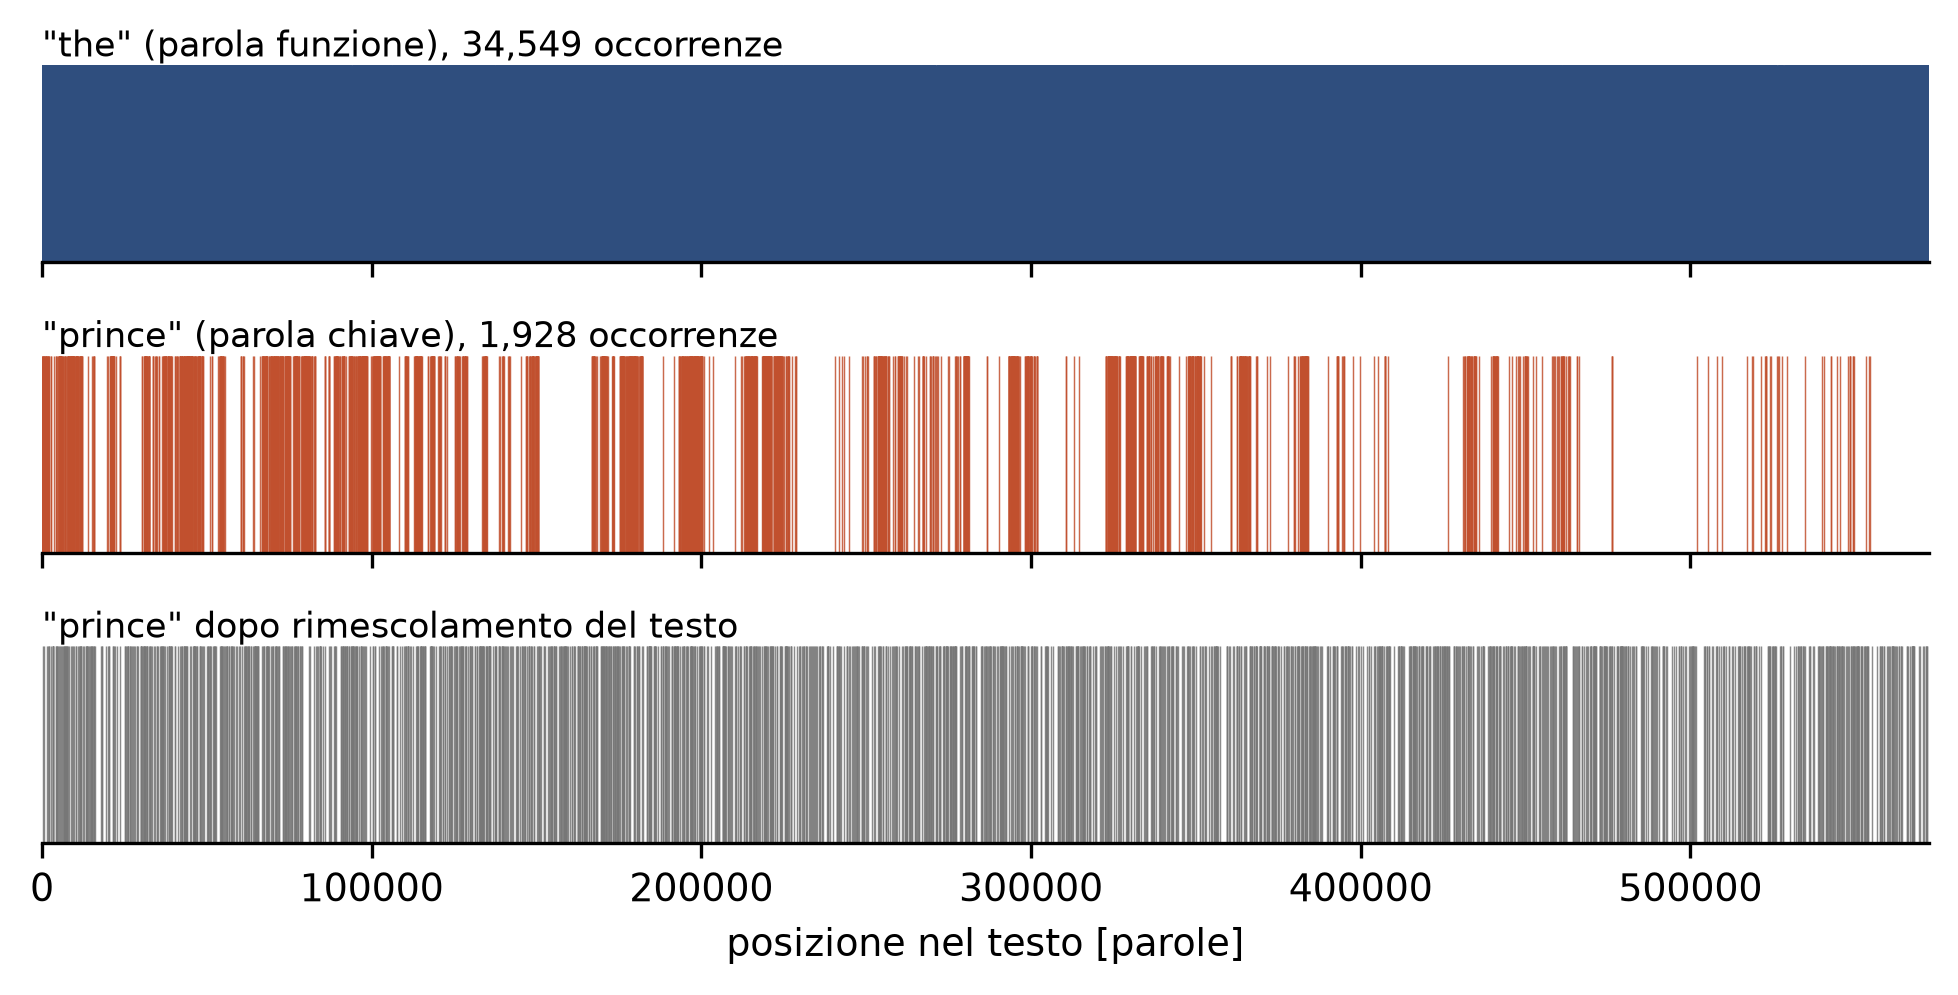
\includegraphics[width=\textwidth]{figure/cap2_burstiness_barcode.png}
  \caption{Posizioni di occorrenza di due parole in \emph{Guerra e pace}. La
  parola funzione \emph{the} riempie il testo in modo uniforme e il pannello
  appare come una banda piena. La parola chiave \emph{prince} si addensa invece
  in gruppi separati da lunghi vuoti, che corrispondono alle porzioni di romanzo
  in cui il personaggio non compare. Il terzo pannello riporta le occorrenze di
  \emph{prince} dopo aver rimescolato le parole del testo: i conteggi sono
  identici, ma i gruppi scompaiono. La struttura visibile nel secondo pannello
  è dunque una proprietà dell'ordine, non delle frequenze.}
  \label{fig:barcode}
\end{figure}

Il fenomeno illustrato dal secondo pannello prende il nome di
\emph{burstiness}: le occorrenze non sono sparse indipendentemente, ma
raggruppate in raffiche separate da intervalli lunghi. Il terzo pannello mostra
perché si tratti di una proprietà dell'ordine e non del vocabolario: il
rimescolamento conserva esattamente il numero di occorrenze, e con esso la legge
di Zipf, ma distrugge la struttura.

Per quantificare il fenomeno si torna alla successione binaria definita
nella~\eqref{eq:osservabile} e si considerano gli intervalli
$\tau_1, \tau_2, \dots$ fra occorrenze consecutive, cioè le distanze in numero
di simboli fra un $1$ e il successivo. La loro distribuzione di probabilità
viene indicata con $p(\tau)$ ed è l'oggetto centrale di questa sezione: tutta
l'informazione sull'ordine che il conteggio delle occorrenze non cattura è
contenuta in $p(\tau)$ e nelle correlazioni fra intervalli successivi.

Il termine di paragone naturale è il processo di Poisson, cioè il processo in
cui ogni posizione ha la stessa probabilità di ospitare un'occorrenza,
indipendentemente da tutte le altre. È il modello del «nessuna struttura»: se le
occorrenze di \emph{prince} fossero poissoniane, il secondo pannello della
Figura~\ref{fig:barcode} sarebbe indistinguibile dal terzo. Per un processo di
Poisson gli intervalli sono distribuiti esponenzialmente e indipendenti fra
loro, e si dimostra che la loro deviazione standard eguaglia la media,
$\sigma_\tau = \langle\tau\rangle$.

Si misura quindi la burstiness con il coefficiente di variazione
\begin{equation}
  \mathrm{cv} \;=\; \frac{\sigma_\tau}{\langle\tau\rangle},
  \label{eq:cv}
\end{equation}
pari a 1 nel caso poissoniano, maggiore di 1 quando le occorrenze si addensano
in raffiche separate da vuoti lunghi e minore di 1 quando sono distribuite in
modo più regolare di quanto il caso comporti. Una misura equivalente, ma
limitata all'intervallo $[-1,1]$ e quindi più comoda per il confronto fra
sequenze diverse, è l'indice proposto da Goh e Barabási~\cite{goh2008},
\begin{equation}
  B \;=\; \frac{\sigma_\tau - \langle\tau\rangle}
                {\sigma_\tau + \langle\tau\rangle} .
  \label{eq:goh}
\end{equation}

% ---------------------------------------------------------------------
\subsection{Le due origini delle correlazioni}
\label{sec:origini}

Il contributo centrale di~\cite{altmann2012} consiste nell'osservare che una
varianza del conteggio che cresce più che linearmente può avere due origini
distinte. Il legame è fornito dallo spettro di potenza a frequenza nulla.

Lo spettro di potenza $S(\omega)$ di una successione descrive come la sua
varianza si distribuisce fra le diverse frequenze $\omega$, ed è la trasformata
di Fourier della funzione di autocorrelazione. Il valore a frequenza nulla,
$S(0)$, raccoglie il contributo delle fluttuazioni più lente, quelle su scale
comparabili con la lunghezza dell'intera successione: è quindi la quantità che
diverge esattamente quando esistono correlazioni a lungo raggio, e che resta
finita quando le correlazioni sono sommabili. Per una successione di occorrenze
descritta dagli intervalli $\tau_i$ vale
\begin{equation}
  S(0) \;=\; \frac{\sigma_\tau^2}{\langle\tau\rangle^3}
  \left(1 + 2\sum_{k\ge1} c_\tau(k)\right),
  \label{eq:eq4}
\end{equation}
dove $c_\tau(k)$ è l'autocorrelazione della successione degli intervalli, cioè
la correlazione fra $\tau_i$ e $\tau_{i+k}$.

La~\eqref{eq:eq4} è il perno dell'intera analisi, perché mostra che $S(0)$ può
divergere in due modi indipendenti. Il primo è la divergenza di $\sigma_\tau$,
cioè una coda pesante di $p(\tau)$: il testo contiene vuoti così lunghi che la
varianza degli intervalli non converge. Il secondo è la non sommabilità di
$c_\tau(k)$, cioè il fatto che gli intervalli siano essi stessi correlati fra
loro. Nella formula resta implicito che cosa questo comporti: $c_\tau(k) > 0$
significa che a un intervallo più lungo della media tende a seguirne un altro
più lungo della media, e quindi che i vuoti si
raggruppano fra loro invece di alternarsi ai riempimenti. Anche con una
$p(\tau)$ a varianza finita, un simile raggruppamento produce fluttuazioni
lente del conteggio e fa divergere la somma.

I due meccanismi sono distinti, perché l'uno riguarda quanto sono lunghi i
vuoti e l'altro come sono disposti, e la~\eqref{eq:eq4} da sola non li separa.

Nei testi reali, di lunghezza finita e con la coda tagliata
(§\ref{sec:coda}), nessuna delle due quantità diverge davvero: ciò che si
misura sono i loro analoghi a finestra finita, e i due null model del
§\ref{sec:null} servono appunto a separarli senza dover decidere quale delle
due divergenze sarebbe realizzata nel limite.

% ---------------------------------------------------------------------
\subsection{I null model A1 e A2}
\label{sec:null}

La separazione si ottiene con due rimescolamenti controllati, costruiti in modo
da distruggere selettivamente uno solo dei due meccanismi.

Il primo, indicato con A1, permuta gli zeri e gli uni della successione binaria.
Conserva soltanto il numero di occorrenze e distrugge tanto la coda di $p(\tau)$
quanto $c_\tau(k)$: è il rimescolamento già illustrato nel terzo pannello della
Figura~\ref{fig:barcode}. Ha funzione di controllo, poiché il risultato è noto a
priori: deve restituire un esponente $\hat\gamma_{A1}$ prossimo a 1, e un valore
diverso segnala un difetto della procedura di misura prima ancora che una
proprietà dei dati.

Il secondo, indicato con A2, permuta fra loro gli intervalli $\tau_i$ senza
alterarne l'insieme. Conserva quindi esattamente $p(\tau)$, e con essa
$\sigma_\tau$, ma distrugge ogni correlazione fra intervalli successivi.
L'esponente risultante $\hat\gamma_{A2}$ isola dunque il solo contributo della
burstiness.

Poiché A2 rimuove un contributo che è di norma non negativo, ci si attende la
disuguaglianza
\begin{equation}
  \hat\gamma \;\ge\; \hat\gamma_{A2},
  \label{eq:disug1}
\end{equation}
che in~\cite{altmann2012} è riportata come regolarità empirica, non come
conseguenza necessaria, e che il §\ref{sec:coda-risultati} verifica
direttamente su tutti i corpora. Fornisce quindi un ulteriore controllo interno
alla misura. Risulta naturale
definire la quota di burstiness
\begin{equation}
  q \;=\; \frac{\hat\gamma_{A2} - 1}{\hat\gamma - 1},
  \label{eq:quota}
\end{equation}
prossima a 1 quando la correlazione proviene interamente dalla coda di $p(\tau)$
e prossima a 0 quando proviene interamente da $c_\tau(k)$: $q$ misura cioè quale
frazione dell'eccesso di correlazione sia attribuibile alla sola burstiness.

Il denominatore della~\eqref{eq:quota} è però piccolo nei corpora poco
correlati, dove $\hat\gamma$ è di poco superiore a 1, e $q$ risulta di
conseguenza uno stimatore rumoroso. Per questa ragione, in questo lavoro $q$
viene calcolata separatamente per ciascun documento e riassunta con mediana e
quartili anziché come rapporto fra medie: si tratta di una scelta metodologica
adottata qui, non di una prescrizione della letteratura, motivata dal fatto che
il rapporto fra due medie non coincide con la media dei rapporti quando il
denominatore ha varianza comparabile al proprio valore.

% ---------------------------------------------------------------------
\subsection{Coda della distribuzione degli intervalli}
\label{sec:coda}

Il legame quantitativo fra burstiness ed esponente di correlazione richiede una
forma esplicita per $p(\tau)$. Assumendo una legge di potenza pura e intervalli
scorrelati si ottiene
\begin{equation}
  p(\tau) \sim \tau^{-\mu}, \quad c_\tau(k) = \delta(k), \quad 2 < \mu < 3
  \;\Longrightarrow\;
  \gamma = 4 - \mu .
  \label{eq:eq8}
\end{equation}
La condizione $2<\mu<3$ individua il regime in cui la media di $\tau$ esiste ma
la varianza diverge, ed è esattamente il regime in cui la~\eqref{eq:cv} non
converge al crescere della lunghezza del testo.

La legge di potenza pura è però un modello idealizzato, e lo stesso
\cite{altmann2012} lo riconosce nel formulare la~\eqref{eq:eq8}. Scendendo
nella gerarchia linguistica i vuoti lunghi vengono spezzati: una lettera che
compone una parola chiave compare anche in tutte le altre parole del testo, e i
lunghi intervalli in cui la parola chiave è assente si riempiono di occorrenze
dovute ad altre parole. Esiste quindi una lunghezza $\tau_c$ oltre la quale gli
intervalli, semplicemente, non si osservano più: è il cut-off che quel lavoro
introduce con questo stesso argomento, senza però stimarlo. Il modello
realistico è la legge di potenza troncata
\begin{equation}
  p(\tau) \;\sim\; \tau^{-\mu}\,e^{-\tau/\tau_c},
  \label{eq:troncata}
\end{equation}
che ha due vantaggi rispetto alla forma pura. Il primo è descrittivo: separa due
proprietà distinte della coda, la pendenza $\mu$ nella regione intermedia e la
distanza $\tau_c$ alla quale la coda viene tagliata, mentre un fit con la sola
legge di potenza le confonde in un unico esponente apparente. Il secondo è che
rende la distribuzione normalizzabile e a varianza finita per ogni $\mu$,
eliminando la necessità di assumere $2<\mu<3$. In presenza di cut-off la
burstiness contribuisce solo per distanze inferiori a $\tau_c$, e
la~\eqref{eq:eq8} non vale più come uguaglianza ma come disuguaglianza,
\[
  \hat\gamma_{A2} \;\le\; 4 - \mu ,
\]
che vincola dall'alto l'esponente misurato sul null model A2.

Nella~\eqref{eq:troncata} $\mu$ e $\tau_c$ agiscono sulla forma della coda in
modo parzialmente sovrapposto: rendere la coda più ripida aumentando $\mu$
produce quasi lo stesso effetto che tagliarla prima riducendo $\tau_c$. Di
conseguenza esistono molte coppie $(\mu, \tau_c)$ diverse fra loro che
descrivono i dati quasi altrettanto bene, cioè che rendono quasi identica la
verosimiglianza, la probabilità di osservare i dati raccolti sotto quei valori
dei parametri. La conseguenza pratica è duplice: gli intervalli di confidenza
vanno calcolati per profilo, esplorando cioè la verosimiglianza al variare di
un parametro con l'altro riottimizzato, e non con la formula asintotica che
presuppone parametri indipendenti; e $\mu$ non va riportato separatamente dal
$\tau_c$ che lo accompagna, perché da solo non identifica la coda.

% ---------------------------------------------------------------------
\subsection{Effetti di dimensione finita}
\label{sec:lunghezza}

Per la legge di potenza pura, quando $\mu<3$ la varianza di $p(\tau)$ diverge e
la stima di $\sigma_\tau$ non converge. Con il taglio della~\eqref{eq:troncata}
i momenti sono invece finiti, ma $\tau_c$ è esso stesso una grandezza che
dipende dalla finestra, e la conseguenza osservabile è la medesima:
la~\eqref{eq:cv} cresce monotonamente con la finestra di osservazione,
poiché finestre più lunghe campionano vuoti più lunghi. Lo stesso vale, in
misura diversa, per l'esponente di Heaps e per il MAPE, come già mostrato nella
Figura~\ref{fig:heaps-finito} del §\ref{sec:heaps}.

La deriva non è un difetto di stima che una procedura migliore potrebbe
eliminare: è una proprietà delle quantità stesse, che su una finestra finita non
hanno un valore limite. Ne discendono vincoli su come i confronti possono essere
condotti, ed è il Capitolo~\ref{cap:metodi} a fissarli, insieme alla misura
dell'entità dell'effetto sui corpora effettivamente impiegati.


% ---------------------------------------------------------------------
\subsection{Entropia degli intervalli}
\label{sec:entropia-intervalli-def}

Il coefficiente di variazione della~\eqref{eq:cv} ha due limiti che il
§\ref{sec:lunghezza} rende evidenti. Il primo è la dipendenza dalla lunghezza
di analisi, che ne impedisce il confronto fra corpora misurati su finestre
diverse. Il secondo è più sottile: $\mathrm{cv}$ è un rapporto e quindi non
cambia se tutti gli intervalli vengono moltiplicati per una costante, ma nei
confronti fra corpora la dilatazione non è uniforme. Quando il tempo si conta in
caratteri, un corpus con frasi mediamente più lunghe produce intervalli più
lunghi ai soli livelli definiti su unità linguistiche, e non a quello dei
caratteri: la scala dei $\tau$ non è la stessa nei due corpora e ogni
differenza ne risente.

Serve quindi una misura di irregolarità che dipenda dalla forma della
distribuzione degli intervalli e non dalla loro scala. Si adotta a questo
scopo l'entropia differenziale del logaritmo degli intervalli, stimata per
spaziature d'ordine con lo stimatore di Vasicek~\cite{vasicek1976}, diminuita
di quella che si otterrebbe da un processo di Poisson con lo stesso numero di
eventi e la stessa media: \begin{equation} J \;=\; h(\ln\tau) \;-\;
h_{\mathrm{Poisson}}(n, \langle\tau\rangle). \label{eq:entropia-intervalli}
\end{equation}

Le due operazioni rispondono ai due limiti. Prendere il logaritmo rende $J$
invariante per dilatazione: moltiplicare tutti i $\tau$ per una costante trasla
$\ln\tau$ senza modificarne l'entropia differenziale, cosicché la diversa
lunghezza delle frasi non produce alcun effetto. Sottrarre il valore poissoniano
fissa lo zero sul processo privo di struttura, come per la~\eqref{eq:cv}, ma con
un vantaggio ulteriore: il termine sottratto viene simulato con lo stesso
stimatore e con gli stessi $n$ e $\langle\tau\rangle$ del dato osservato, per
cui il bias dello stimatore si cancella in larga parte nella differenza invece
di sommarsi.

\paragraph{Fin dove l'invarianza tiene.}
L'argomento appena dato riguarda una distribuzione continua. Gli intervalli fra
occorrenze in un testo sono invece numeri interi, e l'arrotondamento agli interi
non commuta con la dilatazione: comprimere una distribuzione fino a intervalli
di poche unità ne cancella la forma, e $J$ ne risente. Il pannello A della
Figura~\ref{fig:invarianza-J} misura l'entità del fenomeno moltiplicando per una
costante gli intervalli generati da una stessa legge. Per
$\langle\tau\rangle \gtrsim 30$ le curve sono piatte entro due centesimi di bit
e l'invarianza tiene; per $\langle\tau\rangle = 5$ una dilatazione di un fattore
cinquanta sposta $J$ di $0.59$ bit. L'invarianza è dunque asintotica nel valore
medio degli intervalli, non esatta.

La distinzione ha una conseguenza pratica sui livelli linguistici. Ai due
livelli lessicali, dove la diversa lunghezza delle frasi si fa sentire,
l'intervallo medio nei corpora del Capitolo~\ref{cap:risultati2} vale fra $340$
e $1900$ caratteri, quindi in pieno regime asintotico. Ai livelli delle lettere e
degli spazi, dove l'intervallo medio scende sotto la decina, i valori di $J$
risentono della quantizzazione e vanno letti come descrittori relativi, validi
per confrontare corpora misurati allo stesso modo e non come distanze assolute
dal processo di Poisson.

Il pannello B della stessa figura verifica la cancellazione del bias facendo
crescere il numero di intervalli da $30$ a $1000$ su cinque leggi di forma nota.
La deriva residua non supera $0.07$ bit su un intervallo in cui $n$ cambia di un
fattore trentatré, ed è massima sulle distribuzioni log-normali. La
cancellazione è quindi buona ma non completa, e differenze di $J$ inferiori a un
decimo di bit fra sequenze di numerosità molto diversa non sono interpretabili.

\begin{figure}[htbp]
  \centering
  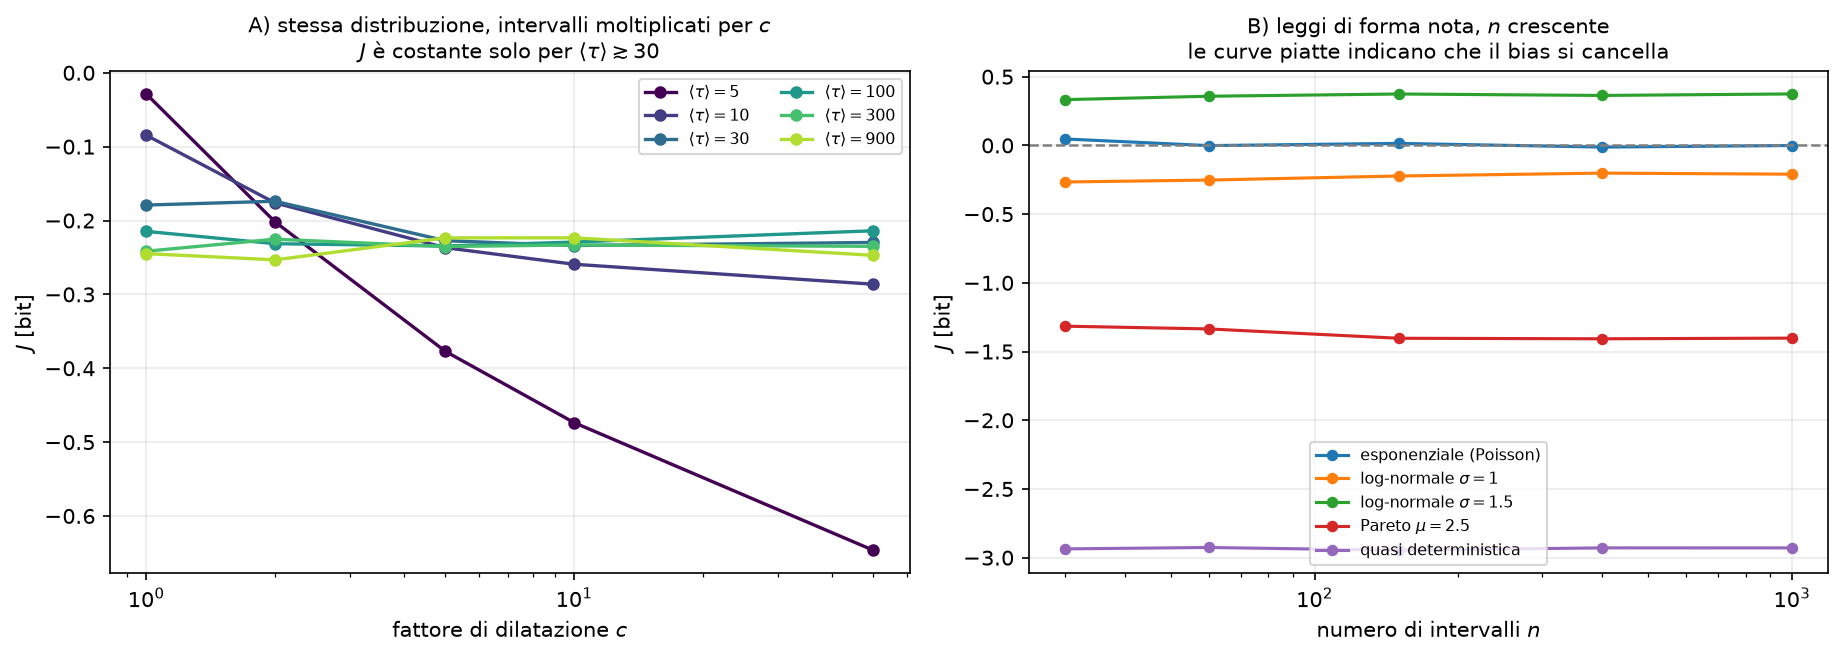
\includegraphics[width=\textwidth]{figure/cap2_invarianza_J.png}
  \caption{Limiti di validità della~\eqref{eq:entropia-intervalli}, misurati
  sullo stimatore effettivamente impiegato. A: intervalli estratti da una stessa
  legge log-normale e moltiplicati per un fattore $c$, per sei valori
  dell'intervallo medio di partenza; una curva piatta indica invarianza. Sotto
  $\langle\tau\rangle \simeq 30$ la quantizzazione agli interi la distrugge. B:
  $J$ su cinque leggi di forma nota al crescere del numero di intervalli; lo
  scostamento fra gli estremi quantifica il bias che la sottrazione del termine
  poissoniano non elimina.}
  \label{fig:invarianza-J}
\end{figure}

Valori positivi di $J$ indicano intervalli distribuiti in modo più irregolare di
un processo di Poisson, valori negativi una regolarità superiore a quella del
caso. La quantità non compare in nessuno dei lavori di riferimento ed è
introdotta qui; il §\ref{sec:entropia-intervalli} ne verifica la stabilità
rispetto alla lunghezza di analisi e la impiega per neutralizzare l'effetto
appena descritto.


% ---------------------------------------------------------------------
\section{Entropia e compressione}
\label{sec:entropia}

Il concetto di disordine di un testo e la nozione di entropia sono già stati
introdotti nel Capitolo~\ref{cap:introduzione}. Trattandosi di un concetto
centrale per questo lavoro, in questa sezione viene definito in modo formale e
ne viene esplicitato il legame con gli algoritmi di compressione, che è lo
strumento con cui l'entropia verrà effettivamente stimata sui testi.

% ---------------------------------------------------------------------
\subsection{Entropia e predicibilità}
\label{sec:entropia-def}

Si consideri una sorgente che emette simboli da un alfabeto finito
$\mathcal{X}$. Per una singola variabile aleatoria $X$ che assume il valore
$x \in \mathcal{X}$ con probabilità $p(x)$, l'entropia di
Shannon~\cite{shannon1948} è
\begin{equation}
  H(X) \;=\; -\sum_{x \in \mathcal{X}} p(x) \log_2 p(x),
  \label{eq:H-singola}
\end{equation}
espressa in bit, e misura l'incertezza media sull'esito dell'estrazione.

I simboli di un testo non sono però indipendenti, e l'entropia di una singola
lettera non descrive la sorgente: sapere che in inglese la lettera più frequente
è \emph{e} dice poco, mentre sapere che dopo \emph{th} segue quasi sempre
\emph{e} dice molto. Occorre quindi considerare blocchi di simboli. Detta
$H(X_1,\dots,X_n)$ l'entropia congiunta di un blocco di lunghezza $n$, definita
dalla~\eqref{eq:H-singola} applicata alla distribuzione congiunta dei blocchi, si
definisce il tasso di entropia della sorgente come
\begin{equation}
  h \;=\; \lim_{n\to\infty} \frac{H(X_1,\dots,X_n)}{n} .
  \label{eq:tasso-entropia}
\end{equation}
Il limite esiste per sorgenti stazionarie ed ergodiche~\cite{cover2006} e
quantifica l'incertezza media per simbolo una volta tenuto conto di tutte le
dipendenze, comprese quelle a lunga distanza. È questa, e non
la~\eqref{eq:H-singola}, la quantità pertinente per un testo.

Il teorema della codifica di sorgente~\cite{cover2006} lega $h$ alla
comprimibilità: il tasso di entropia è un limite inferiore alla lunghezza media
per simbolo di qualunque codifica senza perdita. Stimare l'entropia di un testo
e stimarne la comprimibilità sono quindi, entro le approssimazioni del caso, lo
stesso problema.

Il legame si comprende in modo intuitivo tornando ai casi limite della
Tabella~\ref{tab:tre-regimi}. Un algoritmo di compressione senza perdita opera
sostituendo alle porzioni di testo che si ripetono un riferimento
all'occorrenza precedente, più breve del testo che rimpiazza. Nel testo monotono
il medesimo gruppo di parole ricorre per l'intera lunghezza del documento: dopo
la prima occorrenza tutto il resto è un riferimento, il file compresso è
minuscolo e il tasso di entropia è prossimo a zero, perché il simbolo successivo
è quasi sempre determinato da quelli che lo precedono. Nella sequenza casuale,
al contrario, nessuna porzione si ripete: non esiste nulla cui fare riferimento,
il compressore non guadagna nulla e il tasso di entropia è massimo, perché ogni
simbolo è imprevedibile a partire dai precedenti. Il linguaggio naturale si
colloca fra i due estremi, e la quantità di compressione che ammette è una
misura diretta di quanta struttura possiede.

\paragraph{Stimatori di Lempel--Ziv.}
La stima diretta di $h$ dalla~\eqref{eq:tasso-entropia} per conteggio di blocchi
è impraticabile: il numero di blocchi distinti di lunghezza $n$ cresce
esponenzialmente con $n$, e la dimensione campionaria necessaria a stimarne le
probabilità cresce di conseguenza. Nessun testo reale è abbastanza lungo.

Si ricorre allora agli stimatori della famiglia Lempel--Ziv~\cite{ziv1977},
che aggirano il problema misurando le ripetizioni invece delle probabilità.
L'idea è la seguente: si scorre la successione e, a ogni posizione $i$, si cerca
la più lunga sottostringa che inizi in $i$ e sia già comparsa in precedenza,
detta $\Lambda_i$ la sua lunghezza. In un testo molto ripetitivo i match sono
lunghi, in un testo casuale sono corti. Si dimostra che, per una sorgente
stazionaria ed ergodica, la lunghezza media di tali match cresce come il
logaritmo della finestra esplorata e che
\begin{equation}
  h \;=\; \lim_{n\to\infty}
  \left\langle \frac{\log_2 n}{\Lambda_i} \right\rangle ,
  \label{eq:lz-entropia}
\end{equation}
dove la media è presa sulle posizioni $i$. La~\eqref{eq:lz-entropia} converge
assai più rapidamente del conteggio di blocchi e mantiene buone proprietà anche
in presenza di correlazioni a lungo raggio, che è la ragione per cui viene
adottata qui: le sorgenti considerate in questa tesi hanno, per costruzione,
memoria lunga.

% ---------------------------------------------------------------------
\subsection{Stima della cross-entropia e della divergenza}
\label{sec:crossparsing}

Le quantità introdotte finora descrivono un testo singolo. Per confrontare due
testi occorre la cross-entropia, che misura il costo di codificare un testo
usando la statistica di un altro.

L'algoritmo di cross-parsing di Ziv e Merhav~\cite{ziv1993} estende
la~\eqref{eq:lz-entropia} a due successioni. Data la successione $x$ da
misurare e la successione di riferimento $y$, si scorre $x$ da sinistra a destra
e la si decompone in frasi successive, dove ogni frase è la più lunga
sottostringa che, a partire dalla posizione corrente, compaia da qualche parte
in $y$; raggiunto il punto in cui il match si interrompe, si chiude la frase e
se ne apre una nuova. Il numero di frasi così ottenute viene indicato con
$c(x|y)$ ed è la quantità che misura la somiglianza fra i due testi: se $x$ e
$y$ provengono dalla stessa sorgente, le frasi sono lunghe e poche; se
provengono da sorgenti diverse, i match si interrompono presto e le frasi sono
molte. La stima della cross-entropia è
\begin{equation}
  h(x \,|\, y) \;=\; \frac{c(x|y)\,\log_2 |y|}{|x|},
  \label{eq:crossparsing}
\end{equation}
espressa in bit per simbolo, dove $|x|$ e $|y|$ sono le lunghezze delle due
successioni.

La divergenza di Kullback--Leibler è lo strumento con cui si quantifica quanto
due distribuzioni di probabilità differiscano fra loro. Date due distribuzioni
$P$ e $Q$ sullo stesso alfabeto, essa è definita come
\begin{equation}
  D(P\|Q) \;=\; \sum_{x} P(x) \log_2 \frac{P(x)}{Q(x)}
  \;=\; H_P(Q) - H(P),
  \label{eq:kl-def}
\end{equation}
dove $H_P(Q)$ è la cross-entropia fra le due distribuzioni. La~\eqref{eq:kl-def}
si interpreta come il numero medio di bit sprecati per simbolo codificando una
sorgente $P$ con un codice ottimizzato per $Q$: vale zero se e solo se
$P = Q$ ed è positiva altrimenti.

In termini di successioni, la~\eqref{eq:kl-def} si stima come differenza fra due
cross-entropie: dividendo $x$ in due metà $x_1$ e $x_2$ e prendendo da $y$ un
prefisso $y_1$ della stessa lunghezza di $x_1$, si pone
\begin{equation}
  D(x \,\|\, y) \;=\; h(x_2 \,|\, y_1) \;-\; h(x_2 \,|\, x_1) .
  \label{eq:kl}
\end{equation}
La seconda metà di $x$ viene cioè codificata due volte, una volta usando come
riferimento un testo estraneo e una volta usando la prima metà di $x$ stesso, e
si misura quanto costa in più la prima operazione.

L'appaiamento delle lunghezze dei due riferimenti non è un dettaglio.
La~\eqref{eq:crossparsing} dipende dalla lunghezza del riferimento, poiché un
riferimento più lungo contiene più sottostringhe e produce una cross-entropia
minore a parità di sorgente. Se i due termini della~\eqref{eq:kl} usassero
riferimenti di lunghezza diversa, la differenza conterrebbe un termine spurio
che può superare in modulo il segnale da misurare e produrre stime negative,
impossibili per la~\eqref{eq:kl-def}. Con $|y_1| = |x_1|$ il termine spurio si
cancella, e la costruzione soddisfa la proprietà verificabile $D(x\|x) = 0$
esattamente, impiegata nei capitoli sperimentali come test dello stimatore.

Poiché la~\eqref{eq:kl} non è simmetrica, mentre per confrontare due corpora
serve una quantità che non dipenda da quale dei due venga posto come
riferimento, seguendo~\cite{lippi2019} viene adottata la divergenza
simmetrizzata
\begin{equation}
  D_s(x,y) \;=\; \tfrac{1}{2}\bigl[D(x\|y) + D(y\|x)\bigr].
  \label{eq:kl-sym}
\end{equation}

% ---------------------------------------------------------------------
\subsection{Misure basate su compressione}
\label{sec:compressione}

Le stime della sottosezione precedente usano la compressione come strumento
teorico, attraverso il conteggio delle frasi. Un secondo gruppo di misure,
introdotto in questo contesto da Hadad et al.~\cite{hadad2026}, impiega invece
direttamente un compressore reale come sonda della regolarità strutturale, senza
passare per una stima di entropia.

Detta $C(x)$ la dimensione in byte del testo $x$ dopo la compressione, si
definisce il rapporto di compressione
\begin{equation}
  R_{\mathrm{gzip}}(x) \;=\; \frac{C(x)}{|x|},
  \label{eq:cratio}
\end{equation}
tanto minore quanto più il testo è regolare. Il pedice ricorda l'algoritmo
impiegato e distingue la quantità dal descrittore $R$ della~\eqref{eq:R}.

Da esso derivano la compressione condizionata
$\bigl(C(x+y) - C(x)\bigr)/|y|$, dove $x+y$ indica la concatenazione, che stima
il costo incrementale di codificare la seconda metà di un documento dopo aver
già codificato la prima e misura quindi quanto la seconda metà sia prevedibile
a partire dalla prima; e la distanza normalizzata di compressione~\cite{li2004}
\begin{equation}
  \mathrm{NCD}(x,y) \;=\;
  \frac{C(xy) - \min\{C(x),C(y)\}}{\max\{C(x),C(y)\}} .
  \label{eq:ncd}
\end{equation}
Applicata fra un testo e una sua permutazione, la~\eqref{eq:ncd} misura quanta
parte della comprimibilità dipenda dall'ordine delle parole e non dalla sola
composizione lessicale: è quindi l'analogo, in chiave di compressione, del
confronto fra i pannelli della Figura~\ref{fig:barcode}.


% ---------------------------------------------------------------------
\section{Token ed embedding}
\label{sec:token}

Nel §\ref{sec:scala} si è assunta la parola come unità fondamentale del testo,
in quanto più piccola porzione dotata di significato autonomo per un lettore
umano. Questa scelta non vale più per gli algoritmi di generazione automatica
del testo e, in particolare, per i modelli linguistici di grandi dimensioni.

Si riprenda la frase già usata come esempio,
\emph{Se pensi di comprendere la meccanica quantistica, non comprendi la
meccanica quantistica.} Per un lettore umano essa si scompone come nella
Figura~\ref{fig:scomp-parole}: dodici parole più la punteggiatura, ciascuna
delle quali ha un significato che si può cercare in un dizionario.

\begin{figure}[htbp]
  \centering
  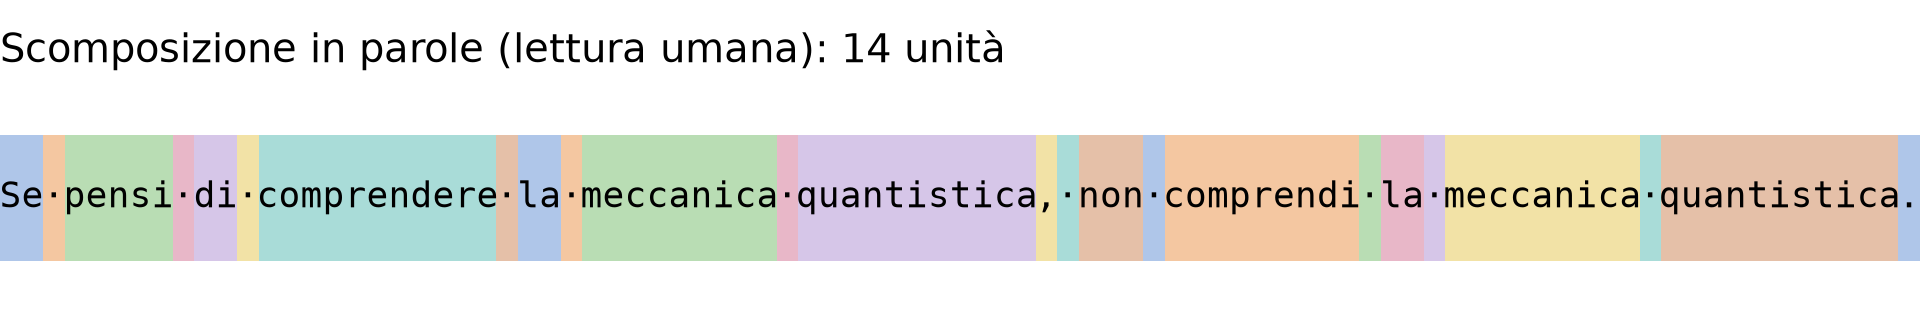
\includegraphics[width=\textwidth]{figure/cap2_scomposizione_parole.png}
  \caption{Scomposizione in parole. Ogni blocco è un'unità dotata di
  significato autonomo; il punto mediano segnala gli spazi.}
  \label{fig:scomp-parole}
\end{figure}

Per un modello linguistico la stessa frase si scompone invece come nella
Figura~\ref{fig:scomp-token}.

\begin{figure}[htbp]
  \centering
  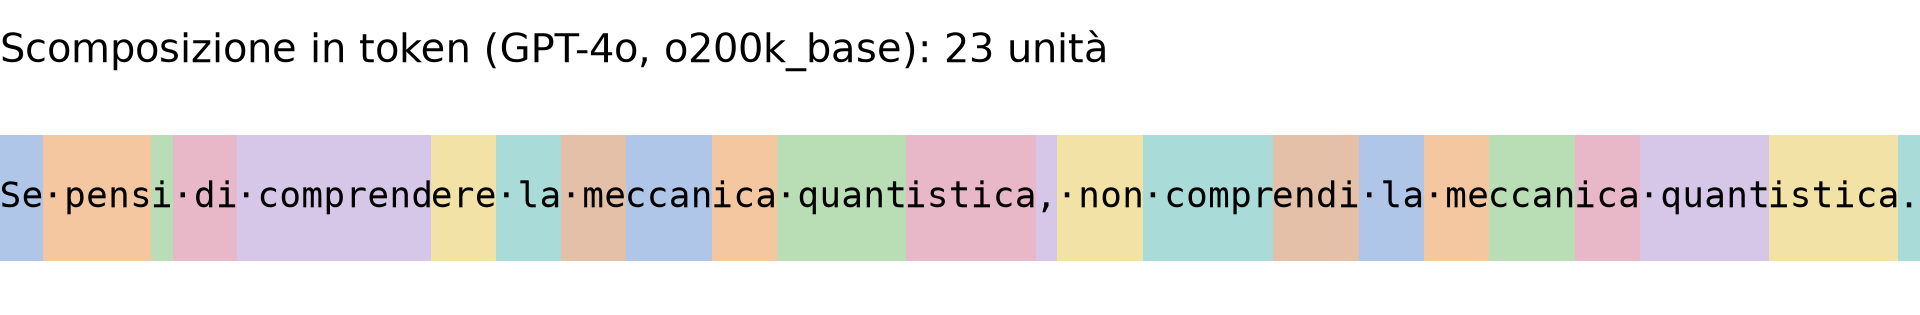
\includegraphics[width=\textwidth]{figure/cap2_scomposizione_token.png}
  \caption{Scomposizione in token della stessa frase, ottenuta con il
  tokenizzatore \texttt{o200k\_base} impiegato da GPT-4o. Le unità sono
  ventitré, non coincidono con le parole e in generale non hanno significato
  autonomo.}
  \label{fig:scomp-token}
\end{figure}

La frase non è divisa né in lettere né in parole, ma in gruppi di lettere
chiamati \emph{token}. Alcuni token coincidono con parole intere
(\texttt{·la}, \texttt{·non}), altri sono frammenti privi di significato
(\texttt{ccan}, \texttt{istica}). Si osservi in particolare la coppia
\emph{comprendere} e \emph{comprendi}: la prima si scompone in
\texttt{·comprend} e \texttt{ere}, la seconda in \texttt{·compr} e
\texttt{endi}. Due forme della stessa radice vengono dunque tagliate in punti
diversi, e il modello non riceve alcuna indicazione esplicita del fatto che
condividano la radice. Lo spazio, inoltre, non separa i token ma vi è
incorporato: la maggior parte dei token inizia con uno spazio, e la
segmentazione del testo in unità precede logicamente qualunque nozione di
parola.

La conversione avviene tramite un algoritmo detto \emph{tokenizzatore}, che
traduce un testo scritto in una qualsiasi lingua e in un qualsiasi alfabeto in
una sequenza di token estratti da un dizionario ampio ma finito, costruito una
volta per tutte a partire da un grande corpus. I dizionari dei tokenizzatori
più diffusi hanno dimensioni dell'ordine di $10^5$ elementi: quello di GPT-4o,
\texttt{o200k\_base}, ne conta \num{200019}; \texttt{cl100k\_base}, impiegato
come unità di analisi nei capitoli sperimentali per le ragioni discusse nel
Capitolo~\ref{cap:metodi}, ne conta \num{100277}; i modelli Qwen2.5 analizzati
in questa tesi ne condividono uno di circa \num{151000} voci. Poiché il
dizionario è finito ma le lingue possibili sono molte, i testi nelle lingue
meno rappresentate nel corpus di costruzione vengono frammentati in un numero
di token assai maggiore rispetto all'inglese.

Proprio come le parole per gli esseri umani, per un modello linguistico sono i
token a trasportare significato. Il significato non è però un'etichetta
associata al token, bensì una posizione: tramite un'operazione detta
\emph{embedding} ogni token viene mappato in un vettore di uno spazio a molte
dimensioni, e la geometria di quello spazio codifica le relazioni fra i token.
Vettori vicini corrispondono a token che compaiono in contesti simili, e
direzioni ricorrenti nello spazio corrispondono a relazioni ricorrenti nel
linguaggio.

La Figura~\ref{fig:embedding} mostra la proprietà su un caso concreto. I vettori
di trenta parole inglesi, appartenenti a cinque famiglie semantiche, sono
proiettati sulle prime due componenti principali dello spazio: le parole di
ciascuna famiglia si dispongono in gruppi distinti, benché la costruzione dei
vettori non abbia mai fatto uso di alcuna classificazione semantica, ma soltanto
delle co-occorrenze osservate in un corpus.

\begin{figure}[htbp]
  \centering
  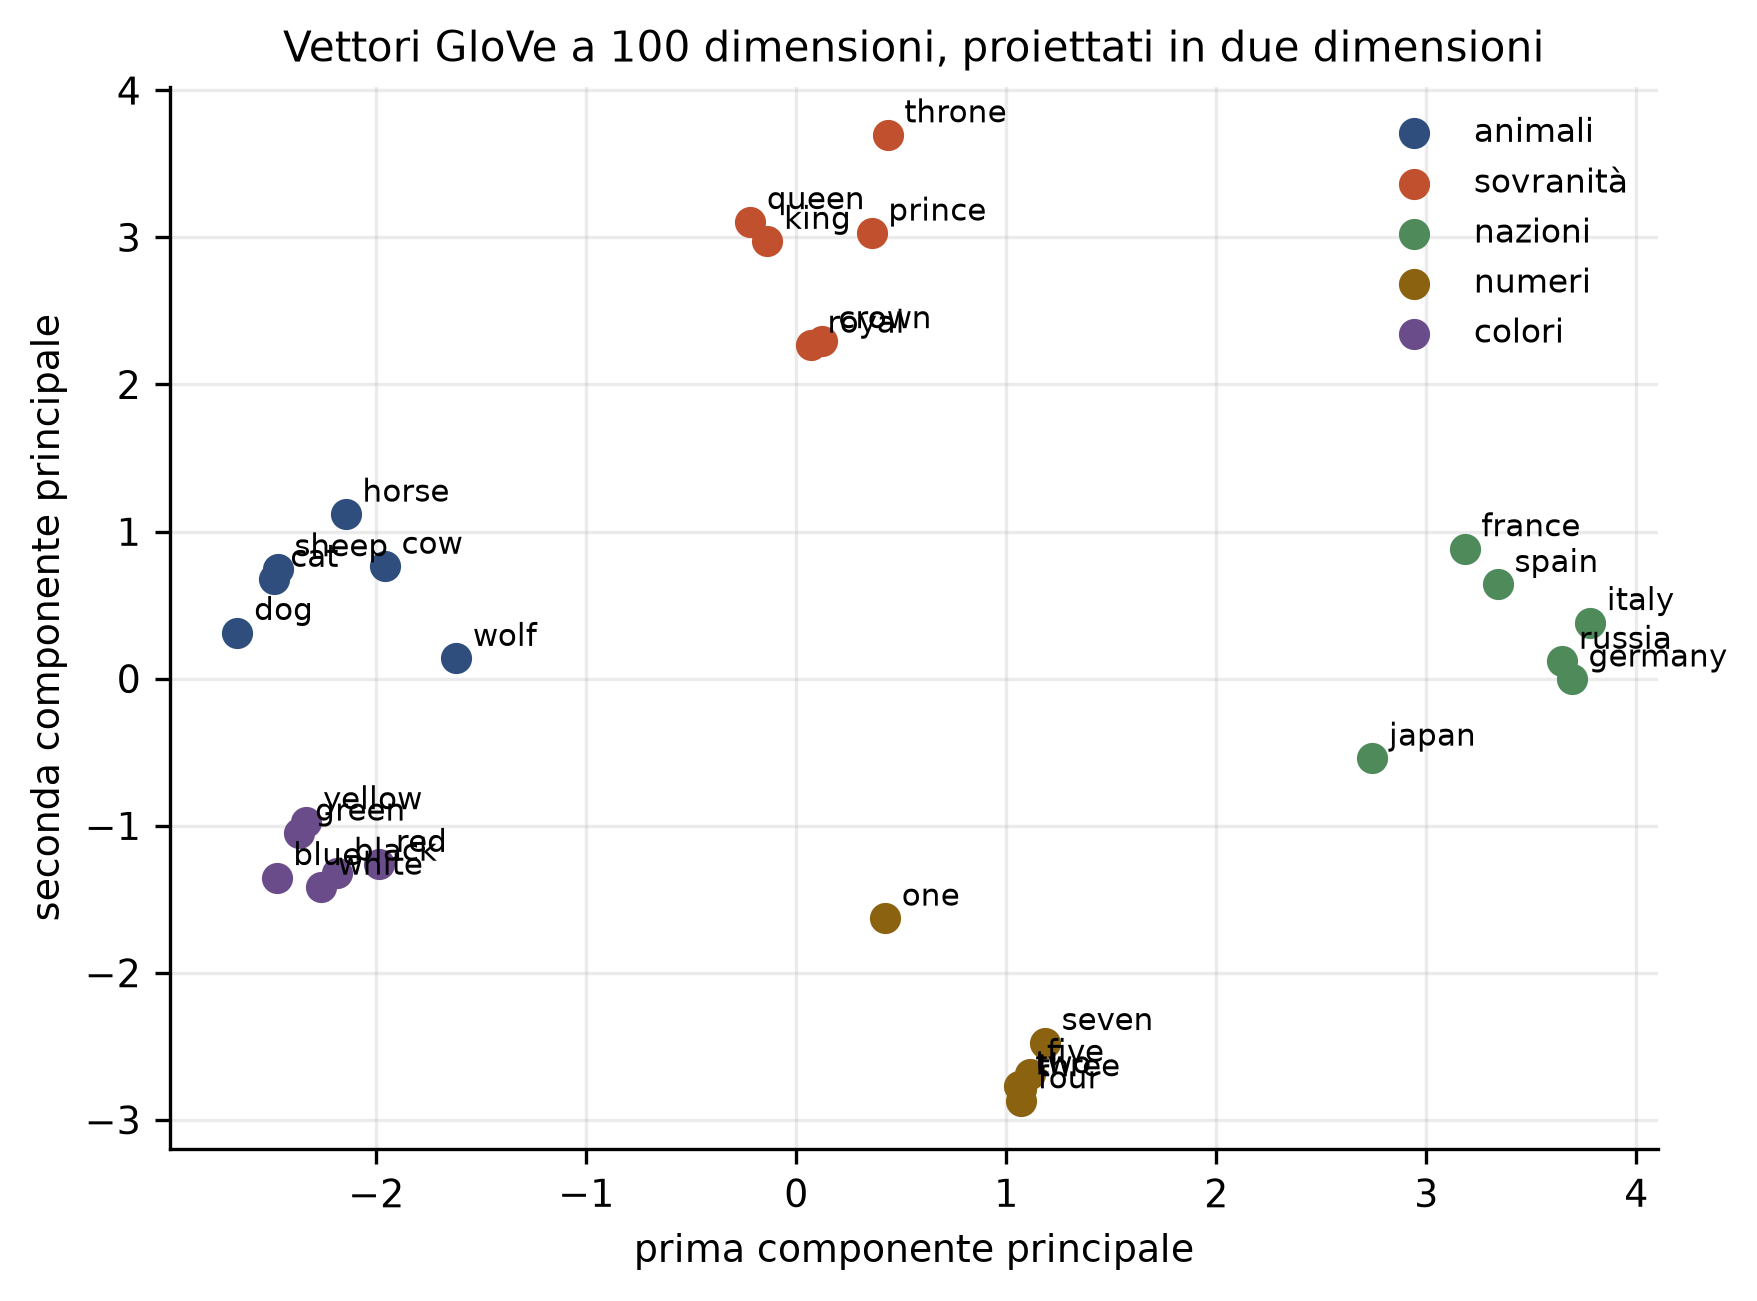
\includegraphics[width=0.82\textwidth]{figure/cap2_embedding_2d.png}
  \caption{Trenta parole inglesi rappresentate dai rispettivi vettori GloVe a
  100 dimensioni, proiettati sulle prime due componenti principali. Le cinque
  famiglie semantiche formano gruppi separati senza che alcuna informazione
  semantica sia stata fornita all'algoritmo. La proiezione conserva soltanto una
  parte della struttura, poiché riduce cento dimensioni a due: la vicinanza
  visibile in figura è una condizione sufficiente, non necessaria, alla
  vicinanza nello spazio originario.}
  \label{fig:embedding}
\end{figure}

I due spazi vettoriali che compaiono in questo lavoro hanno natura diversa. Ogni modello linguistico possiede una propria matrice di embedding,
appresa durante l'addestramento insieme a tutti gli altri parametri, e i cui
vettori non sono direttamente confrontabili fra modelli diversi: fra i modelli
analizzati in questa tesi la dimensione di tale spazio passa da 1536 per il
modello da 1.5 miliardi di parametri a 5120 per quello da 14 miliardi. Gli embedding impiegati nelle analisi di
questa tesi sono invece vettori GloVe a 100 dimensioni, pre-addestrati su un
corpus esterno e identici per tutti i testi esaminati: la scelta è dettata dalla
necessità di misurare i testi generati da modelli diversi con lo stesso metro, e
segue l'impostazione di~\cite{mikhaylovskiy2025states}. Nel
§\ref{sec:traiettoria} tali vettori verranno usati per trasformare un testo in
una traiettoria nello spazio semantico e studiarne l'autocorrelazione.


% ---------------------------------------------------------------------
\section{Generazione autoregressiva e temperatura}
\label{sec:temperatura}

Un modello linguistico autoregressivo, data una sequenza di token $t_{1:m}$,
sceglie il token successivo estraendolo da una distribuzione di probabilità che
dipende dalla sequenza stessa. La probabilità dell'intera sequenza si
decompone per mezzo della regola della catena,
\begin{equation}
  P(t_{1:m}) \;=\; \prod_{k=1}^{m} P(t_k \mid t_{1:k-1}),
  \label{eq:autoregressivo}
\end{equation}
e il modello è addestrato ad approssimare i singoli fattori
$P(t_k \mid t_{1:k-1})$, cioè a prevedere ogni token a partire da tutti quelli
che lo precedono. La generazione consiste nell'applicare ripetutamente questa
previsione, aggiungendo di volta in volta il token estratto alla sequenza che
condiziona l'estrazione successiva.

\paragraph{Origine della distribuzione condizionata.}
Il modo in cui il modello costruisce $P(t_k \mid t_{1:k-1})$ è ciò che
distingue le architetture moderne da quelle precedenti, ed è rilevante per
questo lavoro. I modelli oggi in uso si basano sull'architettura
\emph{transformer}~\cite{vaswani2017}, il cui elemento caratteristico è il
meccanismo di \emph{attenzione}. In esso ogni posizione della sequenza calcola
un peso per ciascuna delle posizioni precedenti e costruisce la propria
rappresentazione come combinazione pesata di quelle: il token in posizione $k$
può quindi attingere direttamente a qualunque token precedente, per lontano che
sia, senza che l'informazione debba propagarsi attraverso le posizioni
intermedie.

È una differenza sostanziale rispetto ai modelli ricorrenti, in cui
l'informazione proveniente da una posizione lontana deve attraversare tutte
quelle interposte e si degrada di conseguenza. Nel transformer il cammino fra
due posizioni qualsiasi ha lunghezza costante, e questo rende l'architettura in
linea di principio capace di rappresentare dipendenze fra porzioni di testo
molto distanti fra loro. È il meccanismo che, negli attuali modelli, potrebbe
dare origine alle correlazioni a lungo raggio descritte nel §\ref{sec:lrc}, e
una delle ragioni per cui ha senso cercarle nel testo generato. La capacità di
rappresentare tali dipendenze non implica però che il modello le riproduca
effettivamente, e l'attenzione opera comunque entro una finestra di contesto
finita: stabilire se le correlazioni siano presenti nel
testo prodotto resta una questione empirica, ed è precisamente quella affrontata
nei capitoli sperimentali.

\paragraph{Temperatura.}
Il modello non produce direttamente probabilità, ma valori reali detti
\emph{logit}, indicati con $u_1,\dots,u_{|\mathcal{L}|}$, uno per ciascun
elemento del dizionario $\mathcal{L}$. Essi vengono convertiti in distribuzione
di probabilità da una funzione softmax riscalata da un parametro
$T$~\cite{ackley1985}:
\begin{equation}
  p(t = \mathcal{L}_l \mid t_{1:i-1}) \;=\;
  \frac{\exp(u_l / T)}{\sum_{l'} \exp(u_{l'} / T)} .
  \label{eq:softmax}
\end{equation}

Il parametro $T$ prende il nome di temperatura, e la denominazione non è una
semplice analogia. Ponendo $E_l = -u_l$, la~\eqref{eq:softmax} coincide con la
distribuzione di Boltzmann $p_l \propto e^{-E_l/T}$ di un sistema a
$|\mathcal{L}|$ stati in equilibrio termico alla temperatura $T$. Questa
identificazione è ciò che giustifica la ricerca, nel testo generato, dei
fenomeni caratteristici dei sistemi termodinamici, e in particolare delle
transizioni di fase discusse nel §\ref{sec:fasi}.

I due limiti sono immediati. Per $T\to0$ la distribuzione si concentra sul token
di logit massimo e la generazione diventa deterministica; per $T\to\infty$ tende
alla distribuzione uniforme sull'intero dizionario, indipendentemente dal
contesto. Fra i due estremi, valori $T<1$ concentrano la massa di probabilità
sugli eventi più probabili, mentre valori $T>1$ la ridistribuiscono verso quelli
meno probabili. La temperatura non modifica dunque ciò che il modello ha
appreso, ma soltanto quanto fedelmente la generazione segue la distribuzione
appresa.

Nella pratica corrente la generazione impiega anche il troncamento della
distribuzione, nelle varianti top-$k$~\cite{fan2018} e
top-$p$~\cite{holtzman2020}, e penalità che scoraggiano la ripetizione. Tutti
questi meccanismi agiscono sulla stessa distribuzione e introducono un secondo
parametro d'ordine, rendendo impossibile attribuire alla sola temperatura il
comportamento osservato. Per questa ragione, e coerentemente con la scelta
esplicita di~\cite{mikhaylovskiy2025zipf}, i dati analizzati in questa tesi sono
stati generati impiegando il solo campionamento per temperatura.


% ---------------------------------------------------------------------
\section{Fasi e stato critico}
\label{sec:fasi}

Una fase di un sistema fisico è uno stato, tipicamente di equilibrio, dotato di
proprietà macroscopiche caratteristiche e stabile in una regione dello spazio
dei parametri; alla frontiera di tali regioni avviene una transizione di fase.
Secondo la classificazione di Ehrenfest~\cite{ehrenfest1933} una transizione di
ordine $n$ è una discontinuità nella derivata $n$-esima dell'energia libera.

Applicare alla lettera questa classificazione al testo generato non è però
possibile. Il sistema considerato non ha un'energia libera di cui prendere
derivate, non è in equilibrio con alcun bagno termico e
non possiede un limite termodinamico, poiché il numero di token di un documento
resta finito. Ciò che rende legittimo il linguaggio delle fasi è la
corrispondenza stabilita nel §\ref{sec:temperatura}: la~\eqref{eq:softmax}
coincide con una distribuzione di Boltzmann in cui i logit giocano il ruolo di
energie e il parametro di campionamento quello di temperatura. La distribuzione
condizionata da cui ogni token viene estratto è dunque, letteralmente, una
distribuzione di Gibbs, e $T$ ne è la temperatura. Quello che resta analogia, e
non identità, è il passaggio dal singolo token al documento: nulla garantisce
che le proprietà collettive di una sequenza generata token per token si
comportino come le proprietà macroscopiche di un sistema all'equilibrio. Il
vocabolario di Ehrenfest viene perciò impiegato in senso descrittivo, per
nominare regioni di comportamento qualitativamente diverso separate da
variazioni rapide, e non per rivendicare una transizione di fase in senso
termodinamico.

Ciò che rende il concetto utile è il comportamento nel punto critico che
separa due fasi: là le correlazioni decadono a legge di potenza e la loro
portata diverge, e molte grandezze osservabili esibiscono lo stesso andamento.
Il criterio inverso, per cui dove compare una legge di potenza si sospetta uno
stato critico, va maneggiato con prudenza, perché distribuzioni a legge di
potenza si generano in molti modi che con la criticità non hanno rapporto, dal
semplice prodotto di variabili aleatorie ai processi di preferential
attachment. Preso da solo, l'andamento a legge di potenza di una quantità non
dimostra nulla. Acquista forza quando più osservabili indipendenti cambiano
regime allo stesso valore del parametro di controllo, ed è in questa forma che
viene impiegato nel §\ref{sec:tstar}: non la legge di potenza di una misura,
ma la convergenza di criteri costruiti per scopi diversi.

Il quadro è stato applicato ai modelli linguistici in~\cite{nakaishi2024}, dove
la temperatura di campionamento separa una fase a bassa temperatura,
caratterizzata da strutture ripetitive, da una ad alta temperatura in cui il
testo è incomprensibile. La tesi sostenuta in quel lavoro è che il linguaggio
naturale si collochi \emph{sul} punto critico fra le due: nello spazio dei
processi stocastici che generano successioni di simboli, il processo
corrispondente a una lingua naturale giacerebbe sulla superficie critica che
separa le due regioni, e un modello addestrato su quella lingua definisce una
famiglia di processi che quella superficie attraversa al variare di $T$. Il
risultato è verificato su modelli da 160 milioni a 2.8 miliardi di parametri, su
sei lingue e su due diverse mappature del testo in successione numerica, il che
ne stabilisce l'indipendenza dalla scala e dalla lingua.

Questa congettura è il punto di contatto più stretto fra il presente lavoro e la
letteratura di fisica statistica sull'argomento, e il
Capitolo~\ref{cap:risultati1} ne fornisce una verifica indipendente: se il
linguaggio naturale è critico, allora la temperatura alla quale il testo
generato somiglia di più a quello umano deve coincidere con quella alla quale il
modello attraversa la transizione, e criteri che misurano proprietà diverse
devono indicarla concordemente.


% ---------------------------------------------------------------------
\subsection{La traiettoria di embedding}
\label{sec:traiettoria}

Il §\ref{sec:token} ha introdotto i vettori di embedding come rappresentazione
del significato. Applicandoli a un testo si ottiene un oggetto geometrico: detta
$(p_1,\dots,p_M)$ la successione delle parole del documento e $v(\cdot)$ la
mappa che associa a una parola il proprio vettore, si pone
\begin{equation}
  \mathbf{m}_i \;=\;
  \begin{cases}
    v(p_i) - \bar{v} & \text{se $p_i$ ha un vettore},\\[2pt]
    \mathbf{0}       & \text{altrimenti},
  \end{cases}
  \label{eq:traiettoria}
\end{equation}
dove $\bar{v}$ è la media dei vettori delle sole parole che ne possiedono uno.
La successione $(\mathbf{m}_1,\dots,\mathbf{m}_M)$ è la traiettoria del testo
nello spazio degli embedding: ogni parola è un punto, e leggere il documento
dall'inizio alla fine equivale a percorrere quella traiettoria.

Due dettagli della~\eqref{eq:traiettoria} incidono sui risultati. Il primo è la
centratura: sottrarre $\bar{v}$ elimina la
direzione media del documento, che altrimenti dominerebbe ogni prodotto scalare
e renderebbe tutte le coppie di parole artificialmente simili. Il secondo è il
trattamento delle parole prive di vettore, alle quali si assegna il vettore
nullo \emph{dopo} la centratura, seguendo~\cite{mikhaylovskiy2025states}: la
posizione nella successione viene così conservata, e con essa la struttura dei
lag, ma la parola non contribuisce ad alcuna correlazione. La conseguenza è che
un testo in cui molte parole non hanno vettore produce una traiettoria fatta in
larga parte di zeri, e le misure che seguono perdono significato prima di
diventare incalcolabili: è la ragione della soglia di validità introdotta più
avanti.

Su questa successione si definisce l'autocorrelazione a distanza $\tau$ come
media della similarità coseno fra i vettori che distano $\tau$ posizioni,
\begin{equation}
  C(\tau) \;=\; \frac{1}{M-\tau} \sum_{i=1}^{M-\tau}
  \frac{\mathbf{m}_i \cdot \mathbf{m}_{i+\tau}}
       {\lVert \mathbf{m}_i \rVert \, \lVert \mathbf{m}_{i+\tau} \rVert},
  \label{eq:acf-embedding}
\end{equation}
con la convenzione che i termini in cui uno dei due vettori è nullo
contribuiscono zero. La~\eqref{eq:acf-embedding} risponde alla domanda: due
parole che distano $\tau$ posizioni tendono a essere semanticamente affini? Vale
$C(\tau) \simeq 0$ quando non c'è alcuna relazione, ed è tanto più vicina a uno
quanto più il testo, a quella distanza, torna a parlare della stessa cosa.

Poiché la~\eqref{eq:acf-embedding} resta calcolabile su qualunque successione,
serve un riferimento che dica quale ampiezza sia distinguibile dal caso. Si
adotta il rimescolamento: si permutano a caso le posizioni della traiettoria, si
ricalcola $C(\tau)$ e si prende il massimo del suo modulo. Il valore così
ottenuto è il livello di rumore del documento, ed è la stessa costruzione dei
null model del §\ref{sec:null}: conserva il contenuto e distrugge l'ordine.
Un'autocorrelazione la cui ampiezza non superi quel livello non è distinguibile
da una successione di parole senza struttura.


% ---------------------------------------------------------------------
\subsection{Le tre fasi}
\label{sec:tre-fasi}

Applicando questo linguaggio al testo generato,
in~\cite{mikhaylovskiy2025states} vengono individuate tre fasi, distinte dal
comportamento di $C(\tau)$.

A bassa temperatura il testo degenera in cicli di ripetizione: la traiettoria
ripassa periodicamente per gli stessi punti, $C(\tau)$ oscilla con periodo pari
alla lunghezza del ciclo e la sua trasformata di Fourier presenta picchi netti.
La quantità che segnala il fenomeno è quindi
\begin{equation}
  \Phi \;=\; \max_{k \ge 1} \bigl\lvert \hat{C}_k \bigr\rvert ,
  \label{eq:periodicita}
\end{equation}
dove $\hat{C}_k$ sono i coefficienti della trasformata discreta di $C(\tau)$. Il
coefficiente $k = 0$ viene escluso perché proporzionale alla media di $C(\tau)$,
cioè al livello complessivo di correlazione e non alla sua periodicità: un testo
uniformemente correlato ma non ciclico ha $\hat{C}_0$ grande e tutti gli altri
coefficienti piccoli. Questa è la fase che, per analogia con gli stati della
materia, viene detta solida. È lo stesso regime in cui, come osservato nel
§\ref{sec:ponte}, la fluttuazione della DFA satura e $\alpha_{\mathrm{DFA}}$
scende verso zero: le due misure segnalano lo stesso fenomeno da due angolazioni
diverse.

La~\eqref{eq:periodicita} si comporta come un parametro d'ordine nel senso che
assume valori grandi in una fase e piccoli nell'altra, ma non si annulla
identicamente fuori dalla fase periodica: su una successione priva di struttura
resta un valore residuo dovuto alle fluttuazioni campionarie. Il
Capitolo~\ref{cap:risultati1} riporta di conseguenza il suo crollo in termini di
ordini di grandezza e non di annullamento.

In una finestra ristretta di temperature $C(\tau)$ decade invece a legge di
potenza: è lo stato critico, quello in cui le leggi di Zipf e di Heaps
introdotte nel §\ref{sec:scala} risultano meglio soddisfatte. Ad alta
temperatura, infine, le correlazioni decadono esponenzialmente e non sussiste
struttura a lungo raggio: è la fase detta amorfa, o gassosa.

Per distinguere le ultime due fasi vengono confrontati due fit
dell'autocorrelazione, uno a legge di potenza e uno esponenziale, tramite il
rapporto dei rispettivi errori~\cite{mikhaylovskiy2023}:
\begin{equation}
  \mathrm{GAPELMAPER} \;=\;
  \frac{\mathrm{MAPE}\bigl(\text{fit a legge di potenza}\bigr)}
       {\mathrm{MAPE}\bigl(\text{fit esponenziale}\bigr)},
  \label{eq:gapelmaper}
\end{equation}
dove il MAPE è quello definito nella~\eqref{eq:mape}. Il rapporto è minore di 1
quando il fit a legge di potenza descrive i dati meglio di quello esponenziale,
e segnala quindi lo stato critico; è maggiore di 1 nella fase amorfa.

La~\eqref{eq:gapelmaper} è un rapporto fra errori di fit, e come tale resta
calcolabile anche quando l'autocorrelazione è indistinguibile dal rumore; in
quel regime, però, il suo valore è privo di contenuto informativo, perché
entrambi i fit descrivono male dati che non contengono alcun segnale.

Le tre fasi, la soglia di periodicità e la condizione di validità si compongono
nella regola seguente. Detti $\kappa$ la quota di parole del documento dotate di
un vettore, $A = \max_\tau \lvert C(\tau)\rvert$ l'ampiezza
dell'autocorrelazione e $\eta$ il livello di rumore stimato per rimescolamento,
un documento viene classificato come
%
\begin{itemize}
  \item \emph{non valutabile}, se $\kappa < \kappa_{\min}$ oppure $A \le \eta$;
  \item \emph{solido}, altrimenti, se $\Phi > \Phi_{\min}$;
  \item \emph{critico}, altrimenti, se $\mathrm{GAPELMAPER} < 1$;
  \item \emph{amorfo} in ogni altro caso.
\end{itemize}
%
L'ordine dei controlli non è indifferente. La condizione di validità viene per
prima perché le altre due misure, su un documento che non la supera, sono numeri
senza referente; la periodicità viene prima del GAPELMAPER perché
un'autocorrelazione periodica non è né una legge di potenza né un esponenziale,
e sottoporla a quel confronto restituirebbe un valore arbitrario. I due valori
di soglia sono fissati nel Capitolo~\ref{cap:risultati1}, dove ne vengono
discussi l'origine e l'effetto.

I due quadri di riferimento non coincidono del tutto.
In~\cite{nakaishi2024} le fasi sono due e ciò che le separa è un punto critico,
cioè un insieme di misura nulla nello spazio dei parametri;
in~\cite{mikhaylovskiy2025states} lo stato critico diventa invece una fase a sé,
dotata di estensione finita. La differenza non è terminologica: nel primo caso
attraversare la transizione con uno sweep a passo finito significa quasi
certamente saltare il punto critico, nel secondo significa attraversare una
regione che si può campionare. Il Capitolo~\ref{cap:risultati1} riporta i dati
pertinenti alla questione senza pretendere di risolverla.


% ---------------------------------------------------------------------
\section{Notazione}
\label{sec:notazione}

Le grandezze introdotte in questo capitolo provengono da lavori che adottano
simboli in conflitto fra loro. La Tabella~\ref{tab:notazione} raccoglie la
notazione seguita in questa tesi, che viene mantenuta senza eccezioni nei
capitoli successivi.

\begin{table}[htbp]
\centering
\small
\begin{tabular}{@{}l>{\raggedright\arraybackslash}p{8.3cm}c@{}}
\toprule
Simbolo & Grandezza & Definita in \\
\midrule
\multicolumn{3}{@{}l}{\itshape Testo e vocabolario} \\
$\mathbf{W}$, $w_t$, $N$ & sequenza di parole, parola in posizione $t$, lunghezza & \eqref{eq:sequenza} \\
$\mathcal{D}$, $\mathcal{D}(t)$ & dizionario e dizionario parziale & §\ref{sec:scala} \\
$f(r)$, $\alpha$ & frequenza della parola di rango $r$, esponente di Zipf & \eqref{eq:zipf} \\
$\gamma_H$ & esponente di Heaps & \eqref{eq:heaps} \\
$R$ & parole nuove nella seconda metà, rapportate alla prima & \eqref{eq:R} \\
MAPE & errore percentuale assoluto medio del fit & \eqref{eq:mape} \\
\addlinespace
\multicolumn{3}{@{}l}{\itshape Correlazioni} \\
$x_k$ & successione binaria generata da un osservabile & \eqref{eq:osservabile} \\
$c(s)$, $\theta$ & autocorrelazione a distanza $s$ e suo esponente di decadimento & \eqref{eq:acf-power} \\
$X(t)$, $\sigma_X^2$, $\gamma$ & conteggio, sua varianza, esponente di crescita & \eqref{eq:sigma} \\
$F(s)$, $\alpha_{\mathrm{DFA}}$ & fluttuazione detrendizzata e suo esponente & \eqref{eq:dfa-alpha} \\
\addlinespace
\multicolumn{3}{@{}l}{\itshape Intervalli e burstiness} \\
$\tau_i$, $p(\tau)$ & intervalli fra occorrenze e loro distribuzione & §\ref{sec:burst} \\
cv, $B$ & coefficiente di variazione, indice di Goh--Barabási & \eqref{eq:cv}, \eqref{eq:goh} \\
$S(0)$, $c_\tau(k)$ & spettro a frequenza nulla, autocorrelazione degli intervalli & \eqref{eq:eq4} \\
$\hat\gamma_{A1}$, $\hat\gamma_{A2}$ & esponenti misurati sui due null model & §\ref{sec:null} \\
$q$ & quota di burstiness & \eqref{eq:quota} \\
$\mu$, $\tau_c$ & esponente di coda e cut-off di $p(\tau)$ & \eqref{eq:troncata} \\
$J$ & entropia degli intervalli, riferita al processo di Poisson & \eqref{eq:entropia-intervalli} \\
\addlinespace
\multicolumn{3}{@{}l}{\itshape Entropia e compressione} \\
$H$, $h$ & entropia di Shannon, tasso di entropia & \eqref{eq:H-singola}, \eqref{eq:tasso-entropia} \\
$c(x|y)$, $h(x|y)$ & frasi del cross-parsing, cross-entropia stimata & \eqref{eq:crossparsing} \\
$D(x\|y)$, $D_s$ & divergenza di Kullback--Leibler e sua versione simmetrizzata & \eqref{eq:kl}, \eqref{eq:kl-sym} \\
$C(x)$, $R_{\mathrm{gzip}}$ & dimensione compressa e rapporto di compressione & \eqref{eq:cratio} \\
NCD & distanza normalizzata di compressione & \eqref{eq:ncd} \\
\addlinespace
\multicolumn{3}{@{}l}{\itshape Generazione e fasi} \\
$u_l$, $T$ & logit del token $l$, temperatura di campionamento & \eqref{eq:softmax} \\
$C(\tau)$ & autocorrelazione della traiettoria di embedding & \eqref{eq:acf-embedding} \\
$\Phi$ & parametro di periodicità di $C(\tau)$ & \eqref{eq:periodicita} \\
GAPELMAPER & rapporto fra gli errori dei due fit dell'autocorrelazione & \eqref{eq:gapelmaper} \\
$N_{\mathrm{eff}}$ & lunghezza comune di analisi & §\ref{sec:scelte} \\
\bottomrule
\end{tabular}
\caption{Notazione adottata in questa tesi.}
\label{tab:notazione}
\end{table}

Per tre simboli la scelta operata qui si discosta da quella di almeno una delle
fonti; la Tabella~\ref{tab:collisioni} riassume le corrispondenze.

\begin{center}
\small
\begin{tabular}{@{}lcccc@{}}
\toprule
Grandezza & Qui & \cite{mikhaylovskiy2025zipf} & \cite{lippi2019} & \cite{altmann2012} \\
\midrule
Esponente di Zipf                  & $\alpha$                & $\alpha$ & $\beta$  & --- \\
Esponente di Heaps                 & $\gamma_H$              & $\beta$  & $\nu$    & --- \\
Esponente della fluttuazione (DFA) & $\alpha_{\mathrm{DFA}}$ & ---      & $\alpha$ & --- \\
Decadimento dell'autocorrelazione  & $\theta$                & ---      & $\gamma$ & $\beta$ \\
Crescita della varianza del conteggio & $\gamma$             & ---      & ---      & $\gamma$ \\
Rapporto di compressione           & $R_{\mathrm{gzip}}$     & ---      & ---      & --- \\
\bottomrule
\end{tabular}
\captionof{table}{Corrispondenza fra la notazione adottata e quella delle fonti primarie,
limitatamente ai simboli per cui le fonti divergono. Il rapporto di compressione
è indicato con $R(x)$ in~\cite{hadad2026}, dove però $R$ non ha il significato
che assume qui.}
\label{tab:collisioni}
\end{center}

Il simbolo $\alpha$ è riservato all'esponente di Zipf, come
in~\cite{mikhaylovskiy2025zipf}, mentre l'esponente della detrended
fluctuation analysis, indicato con $\alpha$ in~\cite{lippi2019}, riceve il
pedice $\mathrm{DFA}$. L'esponente di Heaps è indicato con $\gamma_H$ anziché
con $\beta$ o $\nu$, per lasciare $\gamma$ libero per l'esponente di crescita
della varianza del conteggio, che è la convenzione di~\cite{altmann2012} e
della seconda parte sperimentale. Il decadimento dell'autocorrelazione riceve
infine il simbolo $\theta$, che nessuna delle fonti impiega, poiché entrambe
le lettere che gli sono attribuite in letteratura sono già assegnate. La
lettera $R$ resta al descrittore di~\cite{mikhaylovskiy2025zipf} e il rapporto
di compressione riceve il pedice $\mathrm{gzip}$.

Valgono inoltre le convenzioni seguenti, usate nel seguito senza ulteriore
avviso. Il circonflesso indica una quantità stimata dai dati in contrapposizione
al corrispondente valore teorico, come in $\hat\gamma$. I pedici $A1$ e $A2$
indicano i due null model del §\ref{sec:null}. Il simbolo $|\cdot|$ applicato a
un insieme ne indica la cardinalità e applicato a un testo la lunghezza, in
parole o in byte secondo il contesto. Le medie sono indicate con
$\langle\cdot\rangle$ e si intendono calcolate sull'intero documento salvo
diversa indicazione.

%  Le figure sono attese in figure/; la provenienza e in appendice_figure.tex
% =====================================================================

\chapter{Quadro teorico}
\label{cap:teoria}

In questo capitolo si introducono gli strumenti matematici con cui storicamente
si sono analizzati i testi e che, anche in questo lavoro, ricopriranno un ruolo
centrale: le leggi di scala del vocabolario, le misure di correlazione a lungo
raggio, la statistica degli intervalli fra occorrenze e le stime di entropia
ottenute per compressione.

Successivamente vengono introdotti gli elementi di base del funzionamento dei
modelli linguistici di grandi dimensioni, il linguaggio delle transizioni di
fase con cui alcuni risultati verranno interpretati, e la notazione adottata nel
resto della tesi.


% ---------------------------------------------------------------------
\section{Leggi di scala del vocabolario}
\label{sec:scala}

Come già anticipato, un testo può essere visto come una sequenza di simboli,
siano essi lettere, parole o, come si vedrà nel §\ref{sec:token}, token. La
scelta più naturale per un lettore umano è assumere come unità fondamentale la
parola, in quanto più piccola unità di testo dotata di significato autonomo.

Un testo è quindi una sequenza ordinata di parole
\begin{equation}
  \mathbf{W} \;=\; (w_1, w_2, \dots, w_N),
  \label{eq:sequenza}
\end{equation}
dove $N$ è la lunghezza del testo e l'indice $t = 1,\dots,N$ individua la
posizione di ciascuna parola. L'insieme delle parole distinte che vi compaiono
si dice dizionario e si indica con $\mathcal{D}$; si definisce inoltre il
dizionario parziale $\mathcal{D}(t)$ come l'insieme delle parole distinte
contenute nel prefisso $(w_1,\dots,w_t)$. Valgono per costruzione
$\mathcal{D}(N) = \mathcal{D}$ e $\mathcal{D}(t) \subseteq \mathcal{D}(t+1)$: il
dizionario parziale è una successione non decrescente di insiemi.

A titolo di esempio si consideri la frase
\begin{center}
\emph{Se pensi di comprendere la meccanica quantistica, non comprendi la
meccanica quantistica.}
\end{center}
Con la notazione introdotta si ha $N = 12$, $w_7 = \text{\emph{quantistica}}$ e
\begin{align}
  \mathcal{D}    &= \{\text{se, pensi, di, comprendere, la, meccanica,
                          quantistica, non, comprendi}\}, \\
  \mathcal{D}(6) &= \{\text{se, pensi, di, comprendere, la, meccanica}\} .
\end{align}
Il dizionario completo contiene nove parole distinte a fronte di dodici
occorrenze: le tre ripetizioni di \emph{la}, \emph{meccanica} e
\emph{quantistica} non lo accrescono.

Le due analisi più semplici che si possano condurre su $\mathbf{W}$ sono lo
studio delle frequenze delle singole parole e quello dell'andamento di
$|\mathcal{D}(t)|$ in funzione di $t$. Sono le analisi che hanno portato alla
formulazione delle due leggi empiriche enunciate nel seguito, dovute
rispettivamente a Zipf~\cite{zipf1949} e a Herdan~\cite{herdan1964} e
Heaps~\cite{heaps1978}.

% ---------------------------------------------------------------------
\subsection{Legge di Zipf}
\label{sec:zipf}

Si contino le occorrenze di ciascuna parola distinta e si ordinino le parole per
frequenza decrescente, associando a ognuna il proprio rango $r$: la parola di
rango 1 è la più frequente del testo, quella di rango 2 la seconda, e così via.
Detta $f(r)$ la frequenza della parola di rango $r$, si osserva empiricamente in
tutti i testi naturali che
\begin{equation}
  f(r) \;\propto\; r^{-\alpha}.
  \label{eq:zipf}
\end{equation}
La~\eqref{eq:zipf} prende il nome di legge di Zipf. In coordinate
bilogaritmiche corrisponde a una retta di pendenza $-\alpha$, ed è in tali
coordinate che viene di norma rappresentata e stimata.

La Figura~\ref{fig:zipf} riporta la relazione rango-frequenza per cinque romanzi
in cinque lingue diverse. Le curve sono approssimativamente rettilinee su circa
tre decadi di rango e hanno pendenze molto simili fra loro, nonostante le opere
differiscano per epoca, lingua e lunghezza.

\begin{figure}[htbp]
  \centering
  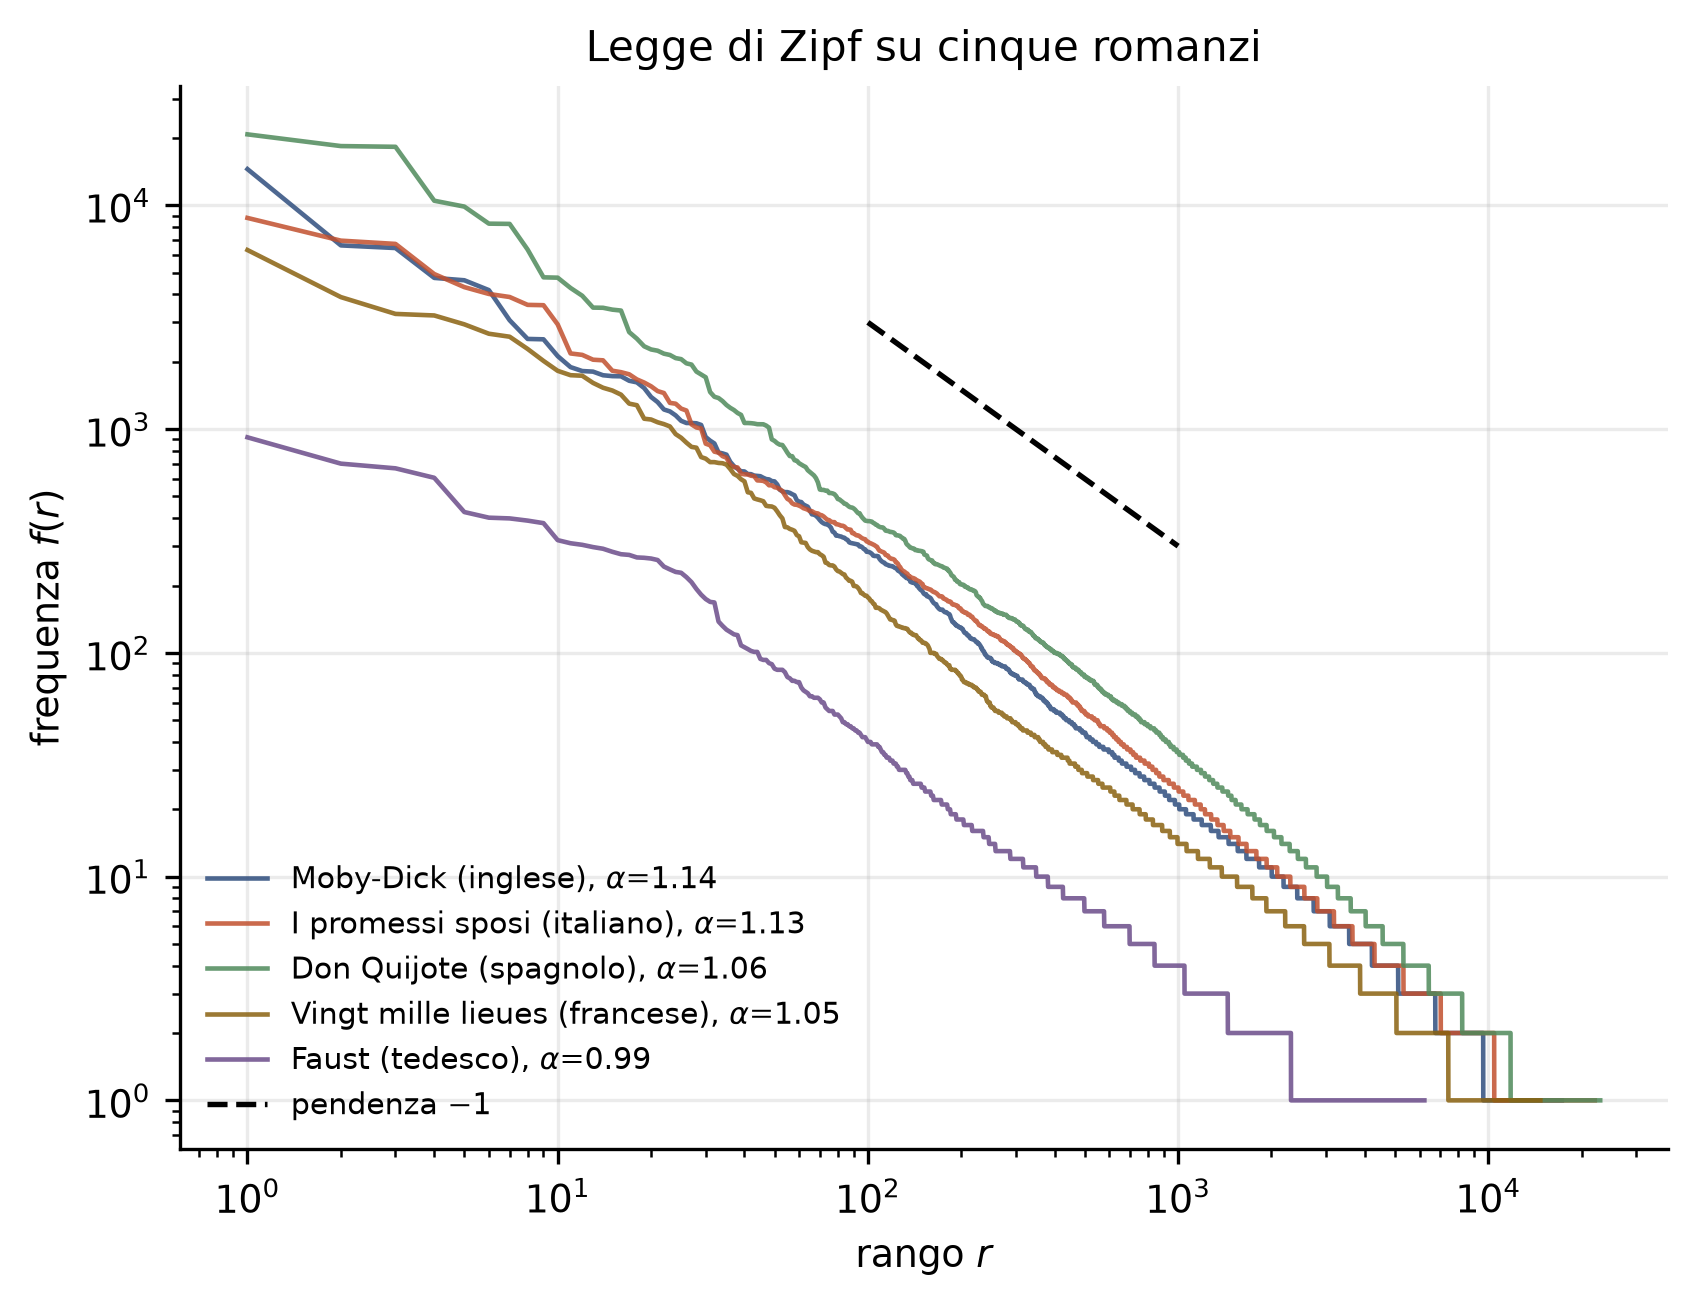
\includegraphics[width=0.82\textwidth]{figure/cap2_zipf_lingue.png}
  \caption{Relazione rango-frequenza per cinque romanzi in altrettante lingue,
  in coordinate bilogaritmiche. Gli esponenti riportati in legenda sono stimati
  per regressione ai minimi quadrati nella finestra di ranghi
  $10^2 \le r \le 10^3$, la stessa impiegata in~\cite{lippi2019}. La retta
  tratteggiata ha pendenza $-1$ ed è riportata come riferimento visivo.}
  \label{fig:zipf}
\end{figure}

Il parametro $\alpha$ risulta positivo e prossimo a 1 nella grande maggioranza
delle lingue esaminate, comprese quelle estinte e quelle costruite
artificialmente. Valori di
$\alpha$ più alti sono sintomo di un vocabolario più povero, poiché un numero
minore di parole esaurisce la maggior parte del testo; valori più bassi
segnalano al contrario una presenza più marcata di parole rare.

I valori misurati sulle cinque opere della Figura~\ref{fig:zipf} sono raccolti
nella Tabella~\ref{tab:zipf-misure}, accanto ai valori medi per lingua riportati
in~\cite{mikhaylovskiy2025zipf} su un corpus di sei opere letterarie in cinque
lingue.

\begin{table}[htbp]
\centering
\small
\begin{tabular}{@{}llrrr@{}}
\toprule
Opera & Lingua & Parole & $|\mathcal{D}|$ & $\alpha$ \\
\midrule
Moby-Dick               & inglese   & \num{219081} & \num{17258} & 1.14 \\
I promessi sposi        & italiano  & \num{239353} & \num{22040} & 1.13 \\
Don Quijote             & spagnolo  & \num{383633} & \num{22943} & 1.06 \\
Vingt mille lieues sous les mers & francese & \num{148923} & \num{14716} & 1.05 \\
Faust                   & tedesco   & \num{30959}  & \num{6221}  & 0.99 \\
\bottomrule
\end{tabular}
\caption{Esponente di Zipf misurato sulle cinque opere della
Figura~\ref{fig:zipf}, con il numero di occorrenze e la dimensione del
dizionario. La stima è condotta sui ranghi $10^2$--$10^3$.}
\label{tab:zipf-misure}
\end{table}

\begin{table}[htbp]
\centering
\small
\begin{tabular}{@{}lcccc@{}}
\toprule
& \multicolumn{2}{c}{$\alpha$ (Zipf)} & \multicolumn{2}{c}{$\gamma_H$ (Heaps)} \\
\cmidrule(lr){2-3}\cmidrule(lr){4-5}
Lingua & parole & token & parole & token \\
\midrule
inglese  & $0.952 \pm 0.072$ & $0.985 \pm 0.054$ & $0.809 \pm 0.027$ & $0.802 \pm 0.024$ \\
tedesco  & $0.959 \pm 0.054$ & $1.024 \pm 0.042$ & $0.846 \pm 0.031$ & $0.793 \pm 0.028$ \\
russo    & $1.043 \pm 0.077$ & $1.009 \pm 0.067$ & $0.916 \pm 0.049$ & $0.805 \pm 0.025$ \\
spagnolo & $0.962 \pm 0.030$ & $1.016 \pm 0.035$ & $0.842 \pm 0.025$ & $0.798 \pm 0.028$ \\
francese & $0.963 \pm 0.033$ & $0.989 \pm 0.042$ & $0.843 \pm 0.020$ & $0.801 \pm 0.018$ \\
\bottomrule
\end{tabular}
\caption{Esponenti medi per lingua riportati in~\cite{mikhaylovskiy2025zipf},
misurati su sei opere letterarie per ciascuna lingua, a livello di parola e di
token. In quel lavoro $\alpha$ è stimato sulla rappresentazione
cumulata della distribuzione anziché sulla relazione rango-frequenza; i due
stimatori coincidono soltanto nel limite $\alpha \to 1$, e i valori non vanno
quindi confrontati direttamente con quelli della
Tabella~\ref{tab:zipf-misure}.}
\label{tab:zipf-letteratura}
\end{table}

Sui testi reali si osservano deviazioni sistematiche dalla~\eqref{eq:zipf}. Su
corpora molto ampi l'esponente resta prossimo a 1 soltanto per le prime migliaia
di parole, mentre la coda continua a seguire una legge di potenza ma con
esponente maggiore~\cite{piantadosi2014}. Le parole più frequenti, inoltre,
mostrano frequenze leggermente inferiori a quelle previste: una deviazione che
Mandelbrot~\cite{mandelbrot1953} corregge introducendo un termine additivo nel
rango,
\begin{equation}
  f(r) \;\propto\; (r + c)^{-\alpha},
  \label{eq:mandelbrot}
\end{equation}
dove la costante $c > 0$ attenua la divergenza della legge di potenza ai ranghi
più bassi, spostando di fatto l'origine dell'asse dei ranghi e rendendo il fit
aderente anche nella regione delle parole più comuni.

\paragraph{Bontà del fit.}
Come si vedrà nei capitoli sperimentali, sui testi generati automaticamente
l'aderenza alla legge di potenza non è garantita. Il solo esponente non è
sufficiente a stabilirla, perché descrive la pendenza media della curva e non la
sua forma: una curva marcatamente incurvata in coordinate bilogaritmiche può
avere la stessa pendenza media di una retta, e restituire quindi un valore di
$\alpha$ del tutto ordinario pur non essendo una legge di potenza. Occorre
perciò una seconda quantità, che misuri quanto i dati si discostino dalla retta
interpolante.

Seguendo~\cite{mikhaylovskiy2025zipf}, la qualità del fit viene stimata con
l'errore percentuale assoluto medio
\begin{equation}
  \mathrm{MAPE} \;=\; \frac{1}{n}\sum_{i=1}^{n}
  \left| \frac{y_i - \hat{y}_i}{y_i} \right|,
  \label{eq:mape}
\end{equation}
dove $n$ è il numero di punti su cui è condotta la regressione, $y_i$ il valore
osservato e $\hat{y}_i$ quello previsto dalla retta interpolante in
corrispondenza dello stesso rango. Il MAPE è nullo per dati perfettamente
allineati e cresce al crescere della distanza relativa dalla retta;
essendo definito su scarti relativi, non dipende dall'unità di misura né
dall'ampiezza delle frequenze, e resta quindi confrontabile fra testi di
lunghezza diversa.

Sul corpus di testi letterari usato in~\cite{mikhaylovskiy2025zipf} il MAPE vale
in media $0.156$ con deviazione standard $0.077$. Nei capitoli sperimentali il
suo minimo in funzione della temperatura di generazione individuerà il regime in
cui il testo prodotto è più vicino a una legge di potenza.

% ---------------------------------------------------------------------
\subsection{Legge di Heaps}
\label{sec:heaps}

Studiando l'andamento di $|\mathcal{D}(t)|$ nei testi letterari emerge una
seconda regolarità, nota come legge di Heaps o, dal nome di chi la formulò per
primo~\cite{herdan1964}, di Herdan--Heaps:
\begin{equation}
  |\mathcal{D}(t)| \;\propto\; t^{\gamma_H}, \qquad \gamma_H \in [0,1] .
  \label{eq:heaps}
\end{equation}
Qui $t$ è la posizione nel testo, misurata in numero di parole,
$|\mathcal{D}(t)|$ la dimensione del dizionario parziale e $\gamma_H$
l'esponente di Heaps. I due estremi dell'intervallo corrispondono a due
comportamenti limite: $\gamma_H = 0$ descrive un dizionario che cessa di
crescere, cioè un testo che non introduce più parole nuove, mentre
$\gamma_H = 1$ descrive un dizionario che cresce proporzionalmente alla
lunghezza, cioè un testo in cui ogni parola è nuova. Poiché il dizionario non
può crescere più rapidamente del testo che lo contiene, si ha necessariamente
$|\mathcal{D}(t)| \le t$, e l'esponente non può eccedere l'unità.

La legge di Heaps quantifica dunque la capacità di un testo di rinnovare il
proprio vocabolario, ed è per questo particolarmente istruttiva se si torna alla
Tabella~\ref{tab:tre-regimi} del Capitolo~\ref{cap:introduzione}. Il primo
esempio, monotono e ripetitivo, cessa rapidamente di accrescere il dizionario;
l'ultimo, in cui i caratteri sono estratti a caso, produce quasi soltanto parole
nuove e fa crescere il dizionario senza saturare. La Figura~\ref{fig:heaps}
mostra le curve dei due casi limite accanto a quelle di tre testi letterari.

\begin{figure}[htbp]
  \centering
  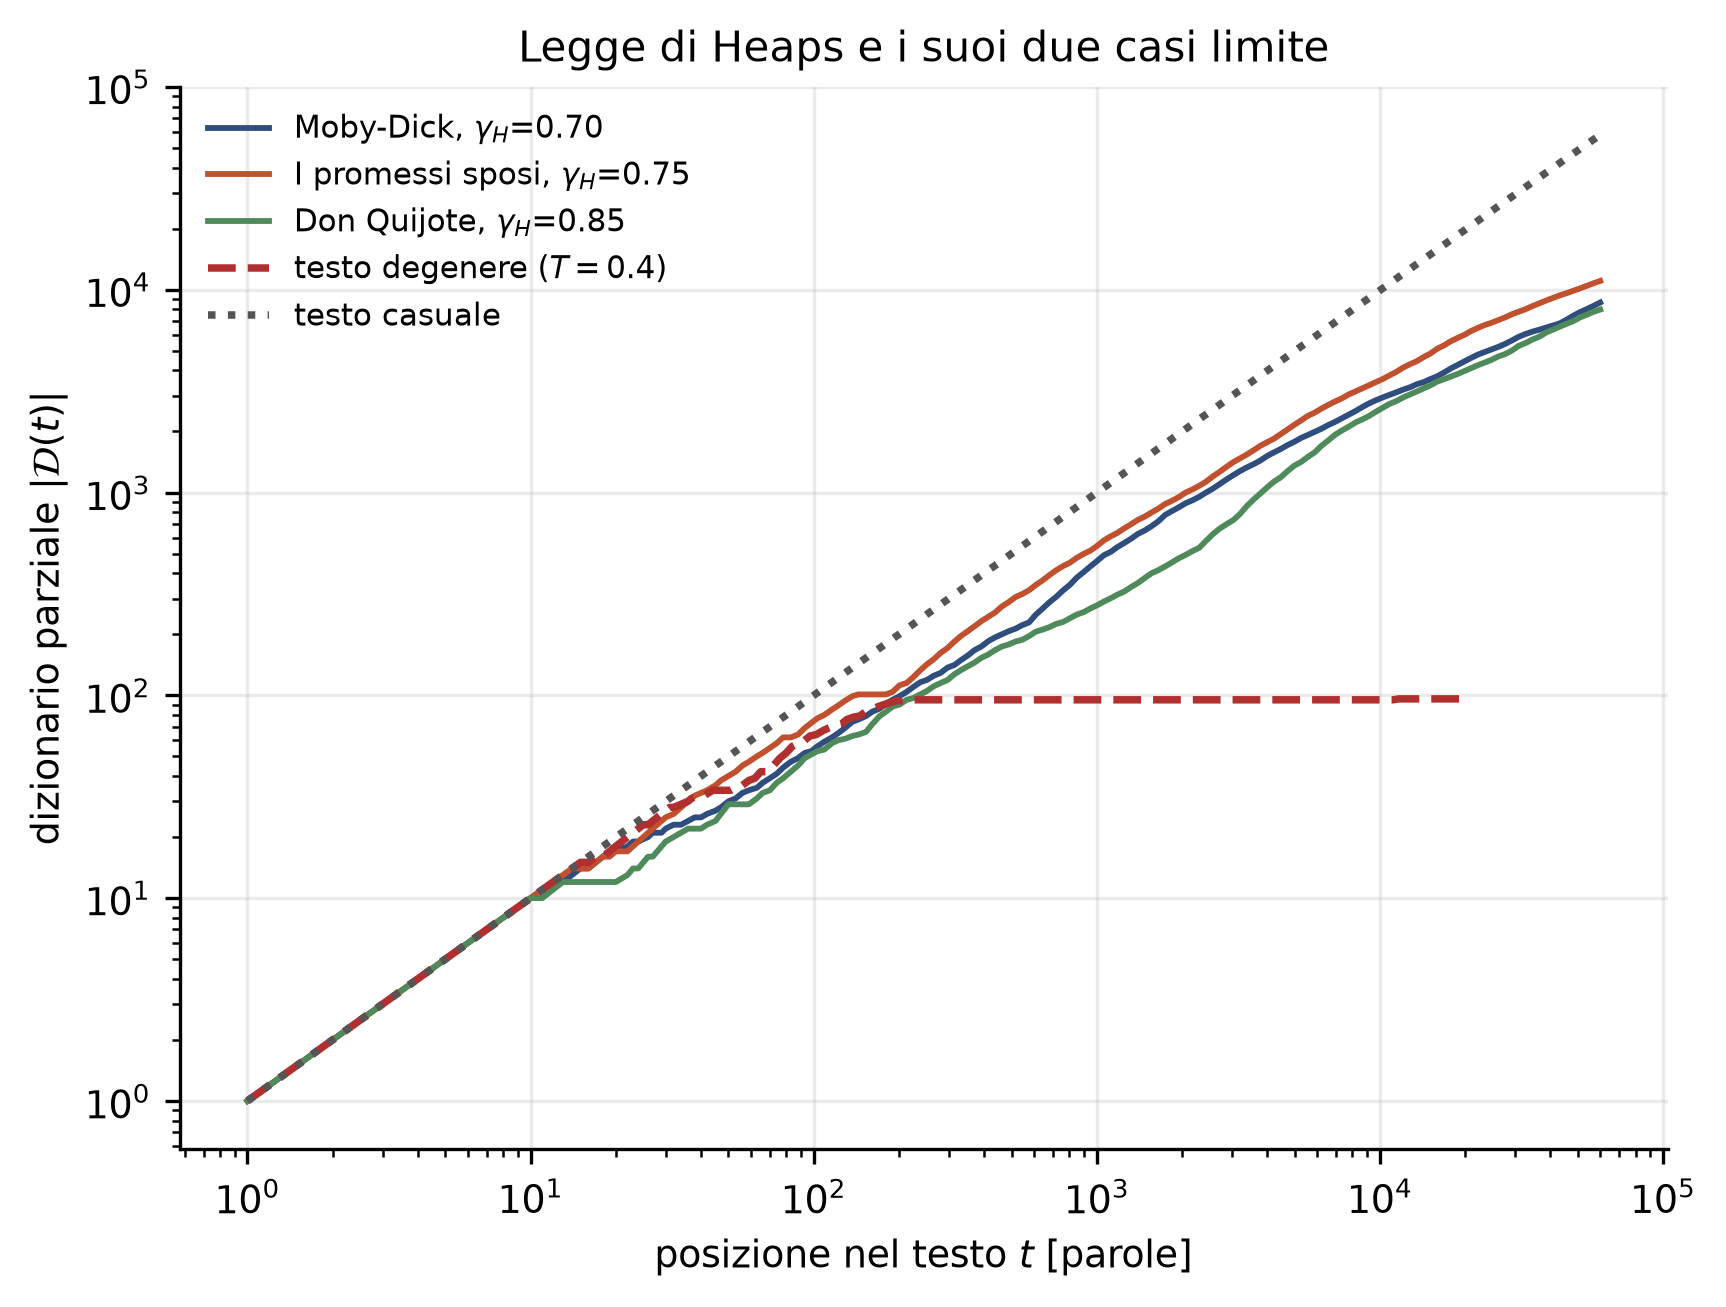
\includegraphics[width=0.82\textwidth]{figure/cap2_heaps_confronto.png}
  \caption{Crescita del dizionario parziale in coordinate bilogaritmiche. Le tre
  curve continue sono testi letterari, con esponente stimato nella regione
  $t > 1000$. La curva tratteggiata è il campione generato a $T = 0.4$ già
  riportato nella Tabella~\ref{tab:tre-regimi}: dopo circa un centinaio di
  parole entra in un ciclo di ripetizione e il dizionario si arresta. La curva
  punteggiata è una sequenza di caratteri casuali, in cui ogni parola è nuova e
  la crescita è esattamente lineare.}
  \label{fig:heaps}
\end{figure}

L'esponente stimato dipende inoltre dall'intervallo su cui viene condotta la
regressione, e quindi dalla lunghezza del testo analizzato. La
Figura~\ref{fig:heaps-finito} mostra l'effetto su tre opere: ripetendo la stima
su prefissi via via più lunghi della stessa opera, $\gamma_H$ decresce in modo
sistematico, di oltre un decimo fra $10^4$ e $10^5$ parole. Il fenomeno è la
prima manifestazione degli effetti di dimensione finita discussi in modo
generale nel §\ref{sec:lunghezza}, ed è già segnalato
in~\cite{mikhaylovskiy2025zipf}, dove si osserva che per $\alpha$ prossimo a 1
la crescita del dizionario è descritta meglio dalla forma $t/\ln t$ che da una
pura legge di potenza. Ai valori di $N$ più bassi la regressione si appoggia a
un intervallo troppo corto e può restituire stime superiori a 1, incompatibili
con il limite teorico: è un artefatto della finestra di fit, non una proprietà
del testo.

\begin{figure}[htbp]
  \centering
  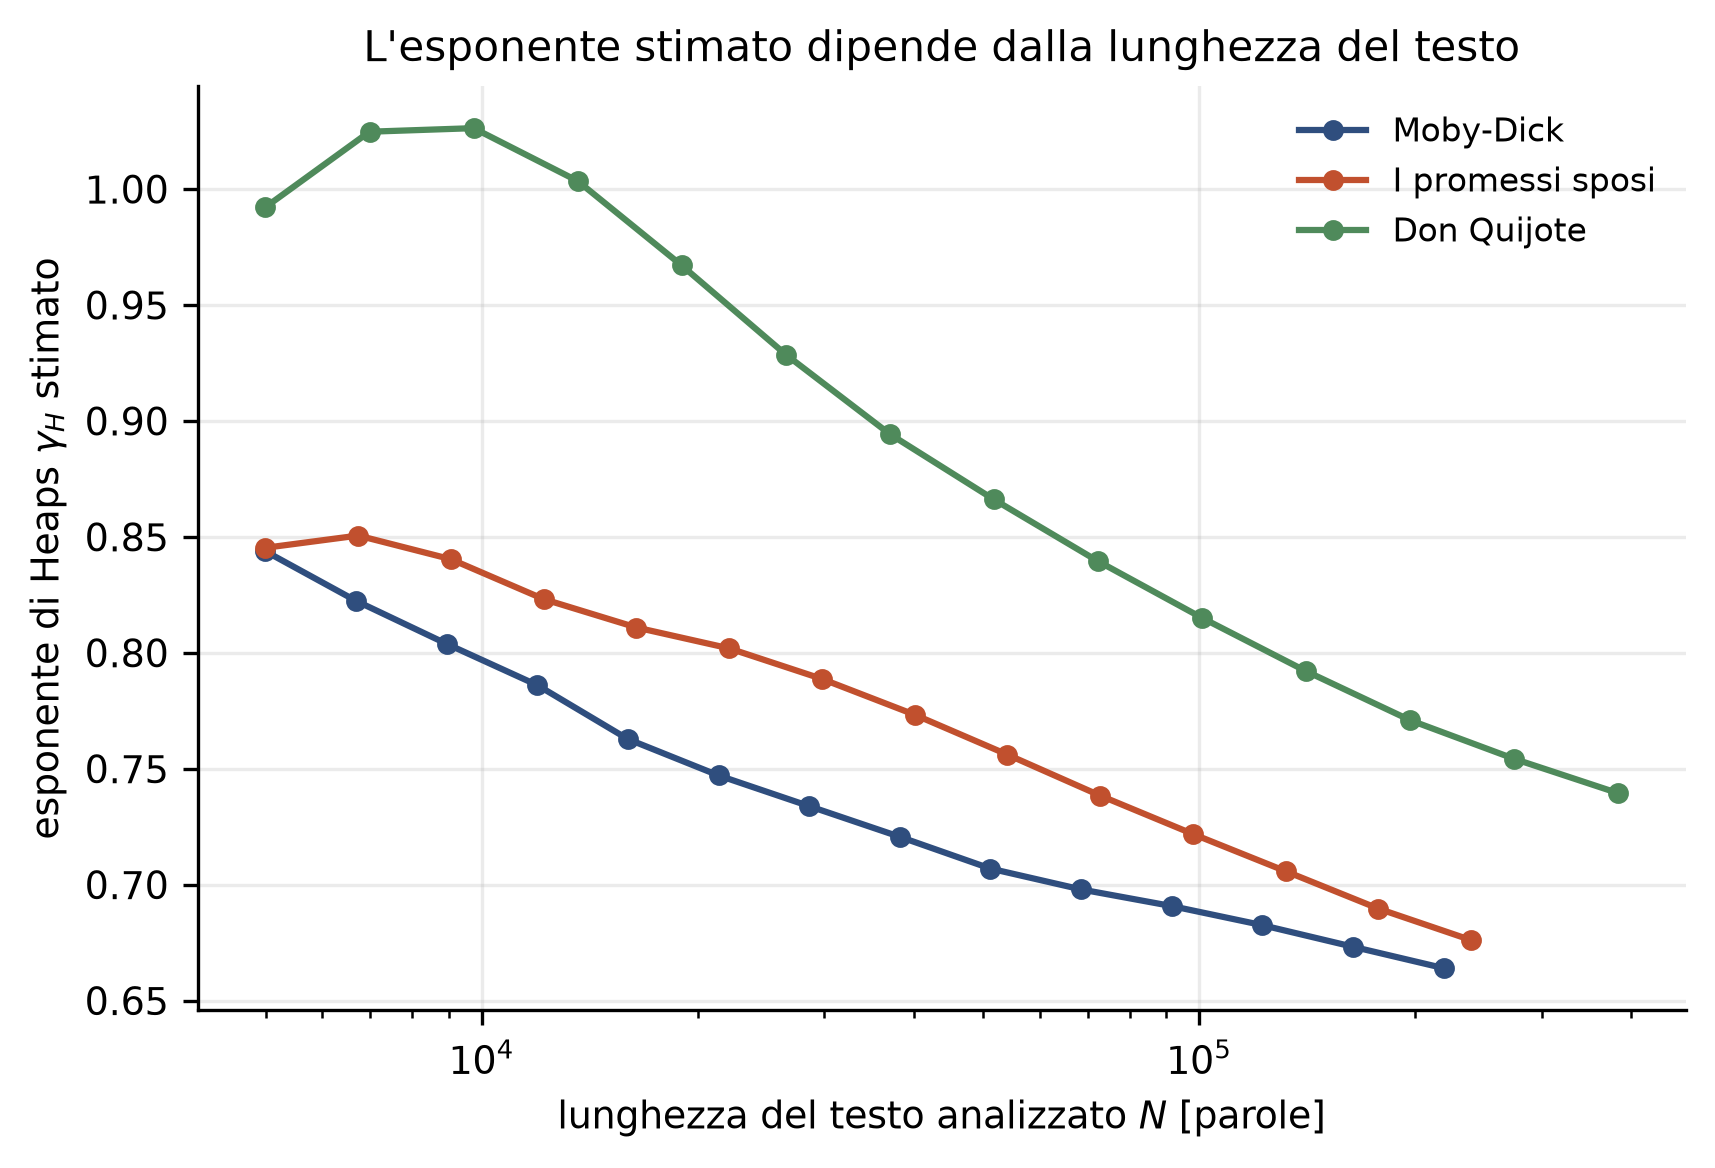
\includegraphics[width=0.78\textwidth]{figure/cap2_heaps_dimensione_finita.png}
  \caption{Esponente di Heaps stimato su prefissi di lunghezza crescente, per tre
  opere in tre lingue diverse, con regressione condotta nella regione $t > 1000$.
  La deriva è sistematica e comune a tutte e tre, ed è quindi una proprietà dello
  stimatore e non di una particolare opera: confrontare esponenti misurati su
  testi di lunghezza diversa non è lecito. Il §\ref{sec:scelte} riprende
  l'effetto su una sola opera, misurandone però l'entità su tutti gli stimatori
  impiegati in questa tesi.}
  \label{fig:heaps-finito}
\end{figure}

\paragraph{Il descrittore $R$.}
Sui testi generati automaticamente la difficoltà è più radicale. A bassa
temperatura di generazione il modello entra in un ciclo di ripetizione e cessa
di produrre parole nuove: la curva $|\mathcal{D}(t)|$ diventa piatta e
la~\eqref{eq:heaps} perde significato. Ad alta temperatura si verifica il caso
opposto, con quasi ogni parola nuova e curva prossima alla linearità. In
entrambe le situazioni la stima di $\gamma_H$ restituisce un numero privo di
contenuto, come mostrano le due curve estreme della Figura~\ref{fig:heaps}.

Per questa ragione in~\cite{mikhaylovskiy2025zipf} viene introdotto un
descrittore che resta definito in ogni regime. Detti $\mathcal{D}_1$ il
dizionario della prima metà del testo e $\mathcal{D}_2$ quello della seconda, si
pone
\begin{equation}
  R \;=\; \frac{|\mathcal{D}_2 \setminus \mathcal{D}_1|}{|\mathcal{D}_1|},
  \label{eq:R}
\end{equation}
cioè il rapporto fra il numero di parole che compaiono per la prima volta nella
seconda metà del testo e il numero di quelle che compaiono per la prima volta
nella prima. Un testo degenerato ha $R$ prossimo a zero, poiché la seconda metà
non introduce nulla di nuovo; un testo in cui ogni parola è nuova ha $R$
prossimo a uno. Sul corpus di opere letterarie intere usato
in~\cite{mikhaylovskiy2025zipf} il valore medio è $R = 0.17$ con deviazione
standard $0.05$.


% ---------------------------------------------------------------------
\section{Correlazioni a lungo raggio}
\label{sec:lrc}

Sia la legge di Zipf sia quella di Heaps ignorano l'ordine dei simboli. Per la
prima l'affermazione è immediata: la~\eqref{eq:zipf} dipende soltanto dai
conteggi delle parole, e un rimescolamento del testo li lascia invariati. Per la
seconda l'invarianza è meno diretta: rimescolando il testo la curva
$|\mathcal{D}(t)|$ cambia realizzazione, perché cambia l'ordine in cui le
parole compaiono per la prima volta, ma il suo andamento medio resta lo stesso, e con esso l'esponente
$\gamma_H$. Entrambe sono quindi proprietà del vocabolario, non della sequenza.

Per misurare le proprietà che dipendono dall'ordine occorre estrarre dal testo
un segnale, cioè una successione finita di valori reali, e studiarne le
correlazioni a scale diverse. La costruzione del segnale non è unica, e ogni
scelta mette in luce aspetti differenti: si può codificare la posizione delle
singole lettere o di classi di lettere, quella delle parole o di classi
grammaticali, oppure la lunghezza delle frasi. In tutti i casi si osserva che il
linguaggio esibisce correlazioni a lungo raggio, con una struttura che si
estende su molti ordini di grandezza~\cite{altmann2012,montemurro2002}.

% ---------------------------------------------------------------------
\subsection{Funzione di autocorrelazione}
\label{sec:acf}

Data una successione $x_1,\dots,x_N$, la funzione di autocorrelazione a distanza
$s$ è
\begin{equation}
  c(s) \;=\; \langle x_n x_{n+s}\rangle
  - \langle x_n\rangle\langle x_{n+s}\rangle ,
  \label{eq:acf}
\end{equation}
dove $\langle\cdot\rangle$ indica la media su tutte le posizioni $n$ compatibili
con la distanza $s$. La forma funzionale di $c(s)$ distingue i regimi di
correlazione.

Se i valori non sono correlati, $c(s)$ è identicamente nulla per $s \neq 0$. Se
$c(s)$ decade esponenzialmente,
$c(s) \sim e^{-s/s_0}$, il segnale si dice correlato a corto raggio: la costante
$s_0$ ha le dimensioni di una distanza e ne fissa la scala caratteristica, nel
senso che oltre poche volte $s_0$ la correlazione è numericamente
indistinguibile da zero. Esiste dunque una distanza tipica oltre la quale due
porzioni di segnale sono indipendenti, e il sistema non possiede struttura al di
là di essa.

Si dice invece che il segnale è correlato a lungo raggio quando il decadimento
segue la legge di potenza
\begin{equation}
  c(s) \;\sim\; s^{-\theta},
  \label{eq:acf-power}
\end{equation}
con $0<\theta<1$. In questo caso non esiste alcuna scala privilegiata: la
funzione~\eqref{eq:acf-power} è invariante di scala, cioè riscalare $s$ di un
fattore costante riscala $c$ di un fattore costante senza modificarne la forma,
e un certo grado di correlazione persiste a tutte le distanze.\footnote{L'esponente
qui indicato con $\theta$ è denotato con $\beta$ in~\cite{altmann2012} e con
$\gamma$ in altra parte della letteratura. Il simbolo è stato cambiato per
evitare la collisione con l'esponente di Heaps e con quello introdotto
nella~\eqref{eq:sigma}.}

La stima diretta di $\theta$ dalla~\eqref{eq:acf-power} è però problematica. Il
segnale è affetto da rumore e, soprattutto, da tendenze di origine esterna che
non sono oggetto di interesse: se la media $\langle x_n\rangle$ differisce fra
la prima e la seconda metà del segnale, come accade proprio quando le
correlazioni sono forti, la~\eqref{eq:acf} risulta distorta. L'esponente va
quindi stimato per via indiretta, e le due sottosezioni seguenti presentano i
due metodi impiegati in questa tesi.

% ---------------------------------------------------------------------
\subsection{Indicatore integrato}
\label{sec:integrato}

Il primo metodo è quello adottato da Altmann, Cristadoro e Degli
Esposti~\cite{altmann2012}, e si applica a segnali binari. Sia dato un testo
come successione simbolica $s = (s_1,\dots,s_N)$. Si definisce una condizione
locale $\mathcal{A}$ che genera la successione binaria
\begin{equation}
  x_k \;=\;
  \begin{cases}
    1 & \text{se $\mathcal{A}$ è soddisfatta in posizione $k$},\\
    0 & \text{altrimenti}.
  \end{cases}
  \label{eq:osservabile}
\end{equation}
L'osservabile può essere la presenza di una data lettera, di una data parola,
oppure l'appartenenza a una classe: per esempio se la lettera in posizione $k$ è
una vocale. L'unità di misura della distanza è il numero di simboli del livello
considerato, ed è questa scelta a rendere confrontabili fra loro una successione
di lettere e una di parole.

Posto
\begin{equation}
  X(t) \;=\; \sum_{j \le t} x_j ,
  \label{eq:conteggio}
\end{equation}
cioè il numero di occorrenze osservate nelle prime $t$ posizioni, si studia la
crescita della varianza del conteggio
\begin{equation}
  \sigma_X^2(t) \;=\; \langle X(t)^2\rangle - \langle X(t)\rangle^2
  \;\simeq\; t^{\gamma}, \qquad \gamma = 2 - \theta .
  \label{eq:sigma}
\end{equation}
La quantità $\sigma_X^2$ è, per costruzione, una somma delle correlazioni a
tutte le distanze inferiori a $t$, e come tale è numericamente assai più stabile
della~\eqref{eq:acf} stimata punto per punto.

Il discrimine fra correlazioni a corto e a lungo raggio non è l'ampiezza di
$c(s)$, ma la sua sommabilità. La~\eqref{eq:conteggio} è formalmente il
cammino percorso da un camminatore che a ogni passo avanza di $x_j$: se i passi
sono indipendenti, o abbastanza rapidamente decorrelati perché $\sum_s c(s)$
converga, vale il teorema del limite centrale e la varianza del cammino cresce
proporzionalmente al numero di passi. Si ha allora diffusione normale,
$\gamma = 1$, esattamente come per il moto browniano. Se invece la somma
diverge, cioè se $\theta \le 1$, i passi restano correlati a ogni scala, il
camminatore tende a proseguire nella direzione già intrapresa e si allontana
dall'origine più rapidamente: la diffusione è anomala e $1 < \gamma < 2$. Il
valore $\gamma = 1$ costituisce dunque il riferimento nullo di tutte le misure
di questo tipo.

La stima di $\gamma$ risente di effetti di tempo finito che la fanno
sottostimare~\cite{altmann2012}: tutti i valori riportati nei capitoli
sperimentali vanno letti come limiti inferiori.

% ---------------------------------------------------------------------
\subsection{Detrended fluctuation analysis}
\label{sec:dfa}

Il secondo metodo è la \emph{detrended fluctuation analysis}, introdotta da
Peng et al.~\cite{peng1994} e applicata ai testi generati automaticamente
in~\cite{lippi2019}. Rispetto all'indicatore integrato presenta il vantaggio
di rimuovere le tendenze locali, e risulta quindi applicabile anche a segnali
non stazionari, cioè segnali le cui proprietà statistiche, tipicamente la
media $\langle x_n \rangle$ o la varianza, non sono costanti lungo la
successione ma derivano lentamente da un estremo all'altro.

La distinzione fra tendenza e correlazione è essenziale, e non riguarda solo
l'origine delle due. Una tendenza è una deriva sistematica e regolare del valore
medio, sovrapposta al segnale da una causa esterna al sistema; una correlazione
è invece una proprietà statistica interna, che lega fra loro le fluttuazioni
attorno a quel valore medio. Il problema pratico è che entrambe producono lo
stesso effetto sulla~\eqref{eq:acf}, gonfiandola a grandi distanze, ed è quindi
necessario eliminare le prime per misurare le seconde. Si potrebbe pensare
sufficiente sottrarre una media mobile di ampiezza fissata, ma in questo modo si
introdurrebbe artificialmente nei dati proprio quella ampiezza come scala
caratteristica, distruggendo le altre.

Il segnale viene costruito codificando ogni carattere del testo con il proprio
rango di frequenza: al carattere più frequente si associa 1, al secondo 2, e
così via. Seguendo~\cite{lippi2019} la codifica avviene a livello di carattere e
conserva punteggiatura, cifre, maiuscole e lettere accentate. Ottenuta la
successione $x_i$ con $i = 1,\dots,N$, la procedura si articola in quattro
passi, qui presentati nella formulazione di~\cite{kantelhardt2001}.

\begin{enumerate}
  \item Si determina il profilo
    \begin{equation}
      Y(i) \;=\; \sum_{k=1}^{i}\bigl(x_k - \langle x\rangle\bigr),
      \label{eq:dfa-profilo}
    \end{equation}
    cioè lo scarto cumulato dalla media. La sottrazione della media non è
    strettamente necessaria, poiché verrebbe comunque eliminata dal detrending.
  \item Si divide il profilo in $N_s = \lfloor N/s \rfloor$ segmenti disgiunti
    di lunghezza $s$.
  \item In ciascun segmento si interpola ai minimi quadrati la tendenza locale,
    ottenendo il polinomio $Y_s(i)$ che approssima il profilo entro quel
    segmento. L'ordine del polinomio determina l'ordine delle tendenze rimosse:
    una DFA di ordine $n$ elimina le tendenze polinomiali fino al grado $n$. In
    questa tesi si impiega l'ordine 1, che rimuove le tendenze lineari locali;
    la robustezza dei risultati rispetto a questa scelta è verificata nel
    §\ref{sec:robustezza}.
  \item Si calcola lo scarto quadratico medio del profilo dalla propria
    tendenza locale, mediando su tutti i segmenti, e si ottiene la funzione di
    fluttuazione
    \begin{equation}
      F(s) \;=\; \left(\frac{1}{N}\sum_{i=1}^{N}
      \bigl(Y(i) - Y_s(i)\bigr)^2\right)^{1/2}.
      \label{eq:dfa-F}
    \end{equation}
\end{enumerate}

La fluttuazione cresce con la lunghezza dei segmenti $s$ e, per un segnale
correlato a lungo raggio, segue la legge di potenza
\begin{equation}
  F(s) \;\sim\; s^{\alpha_{\mathrm{DFA}}} .
  \label{eq:dfa-alpha}
\end{equation}
Per un segnale scorrelato, o correlato a corto raggio, si ha
$\alpha_{\mathrm{DFA}} = 1/2$. Valori superiori indicano correlazioni
persistenti: una fluttuazione positiva tende a essere seguita da un'altra
fluttuazione positiva, e il segnale conserva memoria della propria direzione.
Valori inferiori indicano correlazioni antipersistenti, in cui una fluttuazione
positiva tende a essere seguita da una negativa e il segnale tende a tornare
sui propri passi. Un cammino aleatorio dà $\alpha_{\mathrm{DFA}} = 3/2$: i suoi
incrementi sono scorrelati, ma la successione che ne risulta accumula ogni
deviazione senza riassorbirla, e le fluttuazioni crescono di conseguenza molto
più in fretta. Sul testo letterario di riferimento~\cite{lippi2019} riporta
$\alpha_{\mathrm{DFA}} \simeq 0.65$, contro $0.50$ misurato sulla sua versione
rimescolata: nettamente sopra il riferimento scorrelato e nettamente sotto
quello del cammino aleatorio.

% ---------------------------------------------------------------------
\subsection{Relazione fra i due metodi}
\label{sec:ponte}

I due metodi introdotti misurano la stessa proprietà, e i rispettivi esponenti
sono legati da una relazione semplice. Applicata alla medesima successione,
la~\eqref{eq:dfa-F} coincide, a meno del detrending, con la deviazione standard
del profilo alla scala $s$, cioè $F(s) \simeq \sigma_X(s)$. Elevando al quadrato
e usando la~\eqref{eq:sigma} si ottiene $F(s)^2 \simeq s^{\gamma}$, da cui
\begin{equation}
  \alpha_{\mathrm{DFA}} \;=\; \frac{\gamma}{2} \;=\; 1 - \frac{\theta}{2} .
  \label{eq:ponte}
\end{equation}
La stessa relazione, ricavata per altra via, è riportata
in~\cite{kantelhardt2001}. Nella~\eqref{eq:ponte} $\gamma$ è l'esponente di
crescita della varianza del conteggio definito nella~\eqref{eq:sigma}, mentre
$\theta$ è l'esponente di decadimento dell'autocorrelazione definito
nella~\eqref{eq:acf-power}; i tre esponenti sono dunque tre modi equivalenti di
esprimere la stessa proprietà del segnale.

La~\eqref{eq:ponte} costituisce il ponte fra le due parti sperimentali della
tesi: la diffusione normale $\gamma = 1$, riferimento nullo dell'analisi di
burstiness, corrisponde esattamente al valore $\alpha_{\mathrm{DFA}} = 1/2$,
riferimento nullo dell'analisi sui testi generati. Le due misure non coincidono
esattamente sui dati, poiché la detrended fluctuation analysis rimuove le
tendenze locali mentre l'indicatore integrato no; la differenza fra i due
risultati è informativa proprio quando il segnale non è stazionario.

Un caso limite si presenta con frequenza nei testi generati a bassa
temperatura. Se il testo degenera in un ciclo di ripetizione,
la successione $x_i$ diventa quasi periodica e il profilo~\eqref{eq:dfa-profilo}
oscilla invece di allontanarsi dall'origine: la fluttuazione satura oltre la
lunghezza del periodo e $\alpha_{\mathrm{DFA}}$ scende verso zero. Un esponente
molto basso non segnala quindi assenza di struttura, ma struttura periodica, e
va interpretato congiuntamente a un indicatore diretto di ripetizione.


% ---------------------------------------------------------------------
\section{Burstiness e statistica degli intervalli}
\label{sec:burst}

Le sezioni precedenti permettono di stabilire se un testo possieda correlazioni
a lungo raggio. Questa sezione introduce gli strumenti necessari a stabilire
l'origine di tali correlazioni, che è la domanda posta in~\cite{altmann2012} e
ripresa nella seconda parte sperimentale.

Il punto di partenza è un'osservazione elementare sulla distribuzione delle
parole lungo il testo. Non tutte le parole si distribuiscono allo stesso modo:
alcune ricorrono in modo pressoché uniforme dall'inizio alla fine, altre si
addensano nelle sezioni che trattano l'argomento cui appartengono e sono quasi
assenti altrove. La Figura~\ref{fig:barcode} rende visibile la differenza. Ogni
barra verticale segna una posizione in cui la parola compare; nel primo pannello
la parola è un articolo, nel secondo il nome di un personaggio.

\begin{figure}[htbp]
  \centering
  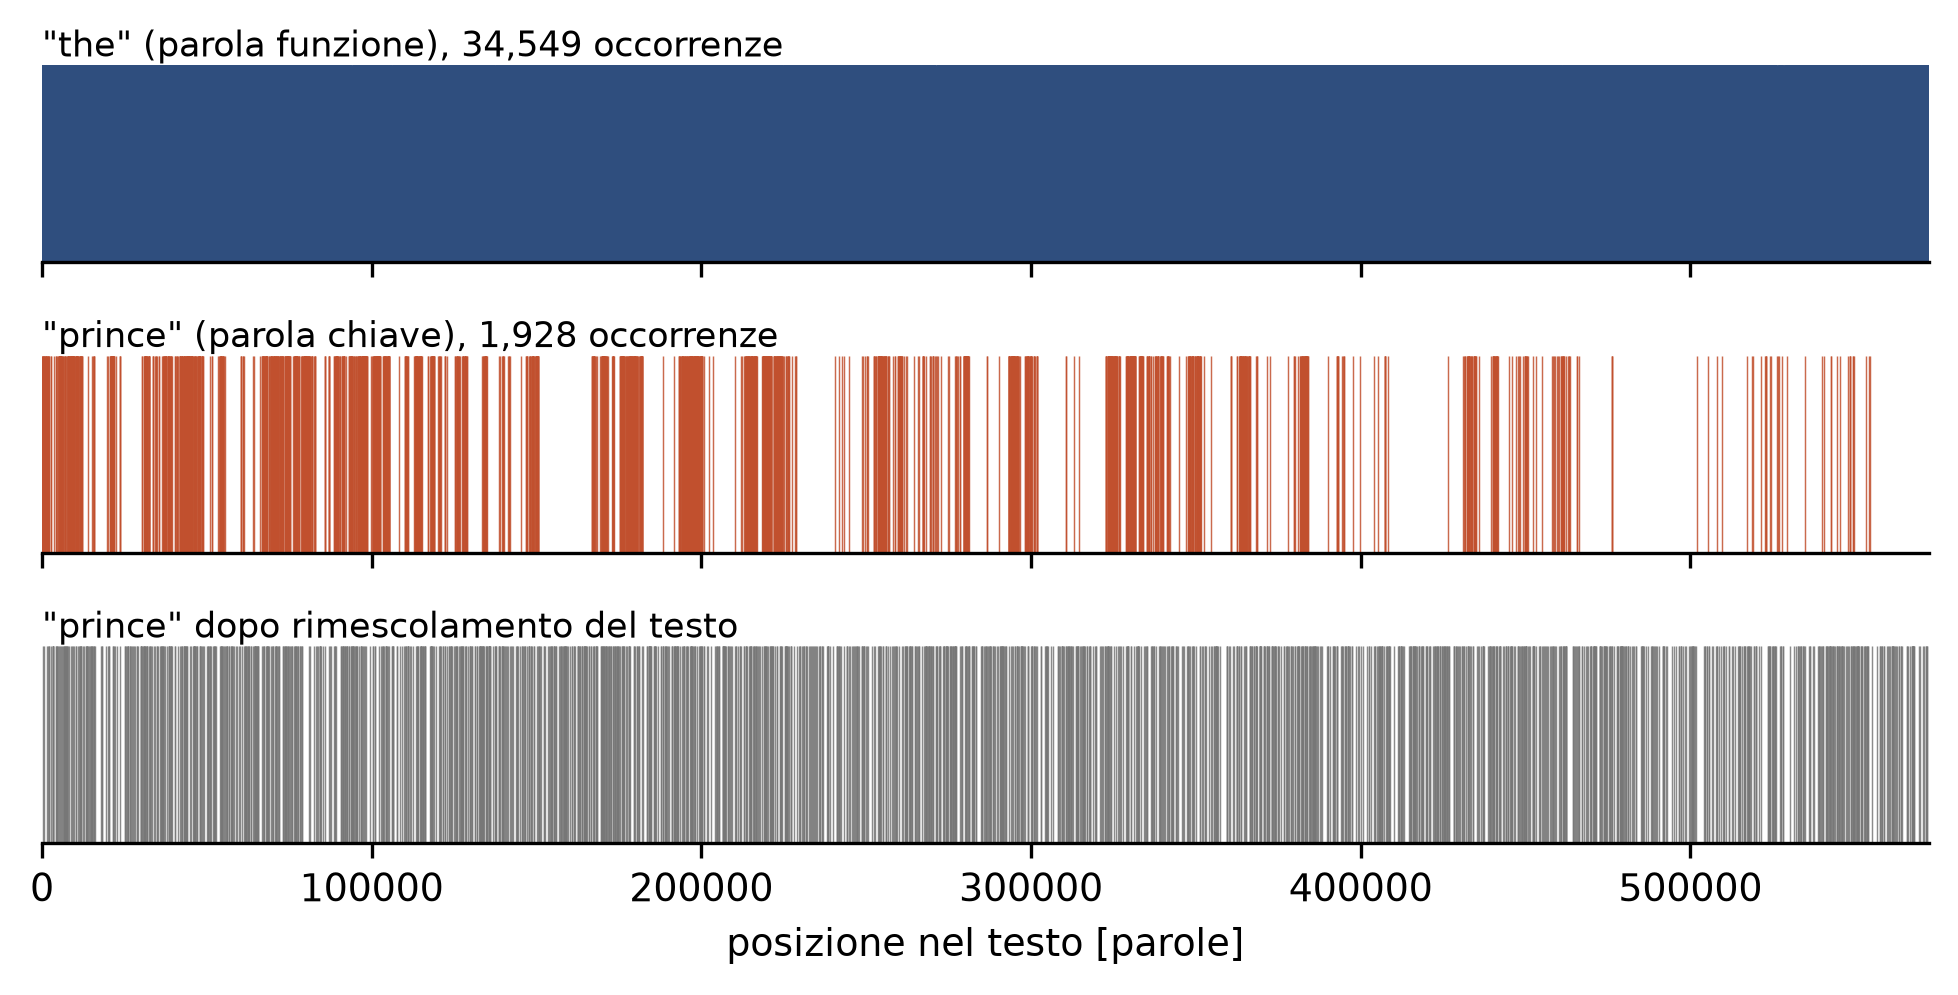
\includegraphics[width=\textwidth]{figure/cap2_burstiness_barcode.png}
  \caption{Posizioni di occorrenza di due parole in \emph{Guerra e pace}. La
  parola funzione \emph{the} riempie il testo in modo uniforme e il pannello
  appare come una banda piena. La parola chiave \emph{prince} si addensa invece
  in gruppi separati da lunghi vuoti, che corrispondono alle porzioni di romanzo
  in cui il personaggio non compare. Il terzo pannello riporta le occorrenze di
  \emph{prince} dopo aver rimescolato le parole del testo: i conteggi sono
  identici, ma i gruppi scompaiono. La struttura visibile nel secondo pannello
  è dunque una proprietà dell'ordine, non delle frequenze.}
  \label{fig:barcode}
\end{figure}

Il fenomeno illustrato dal secondo pannello prende il nome di
\emph{burstiness}: le occorrenze non sono sparse indipendentemente, ma
raggruppate in raffiche separate da intervalli lunghi. Il terzo pannello mostra
perché si tratti di una proprietà dell'ordine e non del vocabolario: il
rimescolamento conserva esattamente il numero di occorrenze, e con esso la legge
di Zipf, ma distrugge la struttura.

Per quantificare il fenomeno si torna alla successione binaria definita
nella~\eqref{eq:osservabile} e si considerano gli intervalli
$\tau_1, \tau_2, \dots$ fra occorrenze consecutive, cioè le distanze in numero
di simboli fra un $1$ e il successivo. La loro distribuzione di probabilità
viene indicata con $p(\tau)$ ed è l'oggetto centrale di questa sezione: tutta
l'informazione sull'ordine che il conteggio delle occorrenze non cattura è
contenuta in $p(\tau)$ e nelle correlazioni fra intervalli successivi.

Il termine di paragone naturale è il processo di Poisson, cioè il processo in
cui ogni posizione ha la stessa probabilità di ospitare un'occorrenza,
indipendentemente da tutte le altre. È il modello del «nessuna struttura»: se le
occorrenze di \emph{prince} fossero poissoniane, il secondo pannello della
Figura~\ref{fig:barcode} sarebbe indistinguibile dal terzo. Per un processo di
Poisson gli intervalli sono distribuiti esponenzialmente e indipendenti fra
loro, e si dimostra che la loro deviazione standard eguaglia la media,
$\sigma_\tau = \langle\tau\rangle$.

Si misura quindi la burstiness con il coefficiente di variazione
\begin{equation}
  \mathrm{cv} \;=\; \frac{\sigma_\tau}{\langle\tau\rangle},
  \label{eq:cv}
\end{equation}
pari a 1 nel caso poissoniano, maggiore di 1 quando le occorrenze si addensano
in raffiche separate da vuoti lunghi e minore di 1 quando sono distribuite in
modo più regolare di quanto il caso comporti. Una misura equivalente, ma
limitata all'intervallo $[-1,1]$ e quindi più comoda per il confronto fra
sequenze diverse, è l'indice proposto da Goh e Barabási~\cite{goh2008},
\begin{equation}
  B \;=\; \frac{\sigma_\tau - \langle\tau\rangle}
                {\sigma_\tau + \langle\tau\rangle} .
  \label{eq:goh}
\end{equation}

% ---------------------------------------------------------------------
\subsection{Le due origini delle correlazioni}
\label{sec:origini}

Il contributo centrale di~\cite{altmann2012} consiste nell'osservare che una
varianza del conteggio che cresce più che linearmente può avere due origini
distinte. Il legame è fornito dallo spettro di potenza a frequenza nulla.

Lo spettro di potenza $S(\omega)$ di una successione descrive come la sua
varianza si distribuisce fra le diverse frequenze $\omega$, ed è la trasformata
di Fourier della funzione di autocorrelazione. Il valore a frequenza nulla,
$S(0)$, raccoglie il contributo delle fluttuazioni più lente, quelle su scale
comparabili con la lunghezza dell'intera successione: è quindi la quantità che
diverge esattamente quando esistono correlazioni a lungo raggio, e che resta
finita quando le correlazioni sono sommabili. Per una successione di occorrenze
descritta dagli intervalli $\tau_i$ vale
\begin{equation}
  S(0) \;=\; \frac{\sigma_\tau^2}{\langle\tau\rangle^3}
  \left(1 + 2\sum_{k\ge1} c_\tau(k)\right),
  \label{eq:eq4}
\end{equation}
dove $c_\tau(k)$ è l'autocorrelazione della successione degli intervalli, cioè
la correlazione fra $\tau_i$ e $\tau_{i+k}$.

La~\eqref{eq:eq4} è il perno dell'intera analisi, perché mostra che $S(0)$ può
divergere in due modi indipendenti. Il primo è la divergenza di $\sigma_\tau$,
cioè una coda pesante di $p(\tau)$: il testo contiene vuoti così lunghi che la
varianza degli intervalli non converge. Il secondo è la non sommabilità di
$c_\tau(k)$, cioè il fatto che gli intervalli siano essi stessi correlati fra
loro. Nella formula resta implicito che cosa questo comporti: $c_\tau(k) > 0$
significa che a un intervallo più lungo della media tende a seguirne un altro
più lungo della media, e quindi che i vuoti si
raggruppano fra loro invece di alternarsi ai riempimenti. Anche con una
$p(\tau)$ a varianza finita, un simile raggruppamento produce fluttuazioni
lente del conteggio e fa divergere la somma.

I due meccanismi sono distinti, perché l'uno riguarda quanto sono lunghi i
vuoti e l'altro come sono disposti, e la~\eqref{eq:eq4} da sola non li separa.

Nei testi reali, di lunghezza finita e con la coda tagliata
(§\ref{sec:coda}), nessuna delle due quantità diverge davvero: ciò che si
misura sono i loro analoghi a finestra finita, e i due null model del
§\ref{sec:null} servono appunto a separarli senza dover decidere quale delle
due divergenze sarebbe realizzata nel limite.

% ---------------------------------------------------------------------
\subsection{I null model A1 e A2}
\label{sec:null}

La separazione si ottiene con due rimescolamenti controllati, costruiti in modo
da distruggere selettivamente uno solo dei due meccanismi.

Il primo, indicato con A1, permuta gli zeri e gli uni della successione binaria.
Conserva soltanto il numero di occorrenze e distrugge tanto la coda di $p(\tau)$
quanto $c_\tau(k)$: è il rimescolamento già illustrato nel terzo pannello della
Figura~\ref{fig:barcode}. Ha funzione di controllo, poiché il risultato è noto a
priori: deve restituire un esponente $\hat\gamma_{A1}$ prossimo a 1, e un valore
diverso segnala un difetto della procedura di misura prima ancora che una
proprietà dei dati.

Il secondo, indicato con A2, permuta fra loro gli intervalli $\tau_i$ senza
alterarne l'insieme. Conserva quindi esattamente $p(\tau)$, e con essa
$\sigma_\tau$, ma distrugge ogni correlazione fra intervalli successivi.
L'esponente risultante $\hat\gamma_{A2}$ isola dunque il solo contributo della
burstiness.

Poiché A2 rimuove un contributo che è di norma non negativo, ci si attende la
disuguaglianza
\begin{equation}
  \hat\gamma \;\ge\; \hat\gamma_{A2},
  \label{eq:disug1}
\end{equation}
che in~\cite{altmann2012} è riportata come regolarità empirica, non come
conseguenza necessaria, e che il §\ref{sec:coda-risultati} verifica
direttamente su tutti i corpora. Fornisce quindi un ulteriore controllo interno
alla misura. Risulta naturale
definire la quota di burstiness
\begin{equation}
  q \;=\; \frac{\hat\gamma_{A2} - 1}{\hat\gamma - 1},
  \label{eq:quota}
\end{equation}
prossima a 1 quando la correlazione proviene interamente dalla coda di $p(\tau)$
e prossima a 0 quando proviene interamente da $c_\tau(k)$: $q$ misura cioè quale
frazione dell'eccesso di correlazione sia attribuibile alla sola burstiness.

Il denominatore della~\eqref{eq:quota} è però piccolo nei corpora poco
correlati, dove $\hat\gamma$ è di poco superiore a 1, e $q$ risulta di
conseguenza uno stimatore rumoroso. Per questa ragione, in questo lavoro $q$
viene calcolata separatamente per ciascun documento e riassunta con mediana e
quartili anziché come rapporto fra medie: si tratta di una scelta metodologica
adottata qui, non di una prescrizione della letteratura, motivata dal fatto che
il rapporto fra due medie non coincide con la media dei rapporti quando il
denominatore ha varianza comparabile al proprio valore.

% ---------------------------------------------------------------------
\subsection{Coda della distribuzione degli intervalli}
\label{sec:coda}

Il legame quantitativo fra burstiness ed esponente di correlazione richiede una
forma esplicita per $p(\tau)$. Assumendo una legge di potenza pura e intervalli
scorrelati si ottiene
\begin{equation}
  p(\tau) \sim \tau^{-\mu}, \quad c_\tau(k) = \delta(k), \quad 2 < \mu < 3
  \;\Longrightarrow\;
  \gamma = 4 - \mu .
  \label{eq:eq8}
\end{equation}
La condizione $2<\mu<3$ individua il regime in cui la media di $\tau$ esiste ma
la varianza diverge, ed è esattamente il regime in cui la~\eqref{eq:cv} non
converge al crescere della lunghezza del testo.

La legge di potenza pura è però un modello idealizzato, e lo stesso
\cite{altmann2012} lo riconosce nel formulare la~\eqref{eq:eq8}. Scendendo
nella gerarchia linguistica i vuoti lunghi vengono spezzati: una lettera che
compone una parola chiave compare anche in tutte le altre parole del testo, e i
lunghi intervalli in cui la parola chiave è assente si riempiono di occorrenze
dovute ad altre parole. Esiste quindi una lunghezza $\tau_c$ oltre la quale gli
intervalli, semplicemente, non si osservano più: è il cut-off che quel lavoro
introduce con questo stesso argomento, senza però stimarlo. Il modello
realistico è la legge di potenza troncata
\begin{equation}
  p(\tau) \;\sim\; \tau^{-\mu}\,e^{-\tau/\tau_c},
  \label{eq:troncata}
\end{equation}
che ha due vantaggi rispetto alla forma pura. Il primo è descrittivo: separa due
proprietà distinte della coda, la pendenza $\mu$ nella regione intermedia e la
distanza $\tau_c$ alla quale la coda viene tagliata, mentre un fit con la sola
legge di potenza le confonde in un unico esponente apparente. Il secondo è che
rende la distribuzione normalizzabile e a varianza finita per ogni $\mu$,
eliminando la necessità di assumere $2<\mu<3$. In presenza di cut-off la
burstiness contribuisce solo per distanze inferiori a $\tau_c$, e
la~\eqref{eq:eq8} non vale più come uguaglianza ma come disuguaglianza,
\[
  \hat\gamma_{A2} \;\le\; 4 - \mu ,
\]
che vincola dall'alto l'esponente misurato sul null model A2.

Nella~\eqref{eq:troncata} $\mu$ e $\tau_c$ agiscono sulla forma della coda in
modo parzialmente sovrapposto: rendere la coda più ripida aumentando $\mu$
produce quasi lo stesso effetto che tagliarla prima riducendo $\tau_c$. Di
conseguenza esistono molte coppie $(\mu, \tau_c)$ diverse fra loro che
descrivono i dati quasi altrettanto bene, cioè che rendono quasi identica la
verosimiglianza, la probabilità di osservare i dati raccolti sotto quei valori
dei parametri. La conseguenza pratica è duplice: gli intervalli di confidenza
vanno calcolati per profilo, esplorando cioè la verosimiglianza al variare di
un parametro con l'altro riottimizzato, e non con la formula asintotica che
presuppone parametri indipendenti; e $\mu$ non va riportato separatamente dal
$\tau_c$ che lo accompagna, perché da solo non identifica la coda.

% ---------------------------------------------------------------------
\subsection{Effetti di dimensione finita}
\label{sec:lunghezza}

Per la legge di potenza pura, quando $\mu<3$ la varianza di $p(\tau)$ diverge e
la stima di $\sigma_\tau$ non converge. Con il taglio della~\eqref{eq:troncata}
i momenti sono invece finiti, ma $\tau_c$ è esso stesso una grandezza che
dipende dalla finestra, e la conseguenza osservabile è la medesima:
la~\eqref{eq:cv} cresce monotonamente con la finestra di osservazione,
poiché finestre più lunghe campionano vuoti più lunghi. Lo stesso vale, in
misura diversa, per l'esponente di Heaps e per il MAPE, come già mostrato nella
Figura~\ref{fig:heaps-finito} del §\ref{sec:heaps}.

La deriva non è un difetto di stima che una procedura migliore potrebbe
eliminare: è una proprietà delle quantità stesse, che su una finestra finita non
hanno un valore limite. Ne discendono vincoli su come i confronti possono essere
condotti, ed è il Capitolo~\ref{cap:metodi} a fissarli, insieme alla misura
dell'entità dell'effetto sui corpora effettivamente impiegati.


% ---------------------------------------------------------------------
\subsection{Entropia degli intervalli}
\label{sec:entropia-intervalli-def}

Il coefficiente di variazione della~\eqref{eq:cv} ha due limiti che il
§\ref{sec:lunghezza} rende evidenti. Il primo è la dipendenza dalla lunghezza
di analisi, che ne impedisce il confronto fra corpora misurati su finestre
diverse. Il secondo è più sottile: $\mathrm{cv}$ è un rapporto e quindi non
cambia se tutti gli intervalli vengono moltiplicati per una costante, ma nei
confronti fra corpora la dilatazione non è uniforme. Quando il tempo si conta in
caratteri, un corpus con frasi mediamente più lunghe produce intervalli più
lunghi ai soli livelli definiti su unità linguistiche, e non a quello dei
caratteri: la scala dei $\tau$ non è la stessa nei due corpora e ogni
differenza ne risente.

Serve quindi una misura di irregolarità che dipenda dalla forma della
distribuzione degli intervalli e non dalla loro scala. Si adotta a questo
scopo l'entropia differenziale del logaritmo degli intervalli, stimata per
spaziature d'ordine con lo stimatore di Vasicek~\cite{vasicek1976}, diminuita
di quella che si otterrebbe da un processo di Poisson con lo stesso numero di
eventi e la stessa media: \begin{equation} J \;=\; h(\ln\tau) \;-\;
h_{\mathrm{Poisson}}(n, \langle\tau\rangle). \label{eq:entropia-intervalli}
\end{equation}

Le due operazioni rispondono ai due limiti. Prendere il logaritmo rende $J$
invariante per dilatazione: moltiplicare tutti i $\tau$ per una costante trasla
$\ln\tau$ senza modificarne l'entropia differenziale, cosicché la diversa
lunghezza delle frasi non produce alcun effetto. Sottrarre il valore poissoniano
fissa lo zero sul processo privo di struttura, come per la~\eqref{eq:cv}, ma con
un vantaggio ulteriore: il termine sottratto viene simulato con lo stesso
stimatore e con gli stessi $n$ e $\langle\tau\rangle$ del dato osservato, per
cui il bias dello stimatore si cancella in larga parte nella differenza invece
di sommarsi.

\paragraph{Fin dove l'invarianza tiene.}
L'argomento appena dato riguarda una distribuzione continua. Gli intervalli fra
occorrenze in un testo sono invece numeri interi, e l'arrotondamento agli interi
non commuta con la dilatazione: comprimere una distribuzione fino a intervalli
di poche unità ne cancella la forma, e $J$ ne risente. Il pannello A della
Figura~\ref{fig:invarianza-J} misura l'entità del fenomeno moltiplicando per una
costante gli intervalli generati da una stessa legge. Per
$\langle\tau\rangle \gtrsim 30$ le curve sono piatte entro due centesimi di bit
e l'invarianza tiene; per $\langle\tau\rangle = 5$ una dilatazione di un fattore
cinquanta sposta $J$ di $0.59$ bit. L'invarianza è dunque asintotica nel valore
medio degli intervalli, non esatta.

La distinzione ha una conseguenza pratica sui livelli linguistici. Ai due
livelli lessicali, dove la diversa lunghezza delle frasi si fa sentire,
l'intervallo medio nei corpora del Capitolo~\ref{cap:risultati2} vale fra $340$
e $1900$ caratteri, quindi in pieno regime asintotico. Ai livelli delle lettere e
degli spazi, dove l'intervallo medio scende sotto la decina, i valori di $J$
risentono della quantizzazione e vanno letti come descrittori relativi, validi
per confrontare corpora misurati allo stesso modo e non come distanze assolute
dal processo di Poisson.

Il pannello B della stessa figura verifica la cancellazione del bias facendo
crescere il numero di intervalli da $30$ a $1000$ su cinque leggi di forma nota.
La deriva residua non supera $0.07$ bit su un intervallo in cui $n$ cambia di un
fattore trentatré, ed è massima sulle distribuzioni log-normali. La
cancellazione è quindi buona ma non completa, e differenze di $J$ inferiori a un
decimo di bit fra sequenze di numerosità molto diversa non sono interpretabili.

\begin{figure}[htbp]
  \centering
  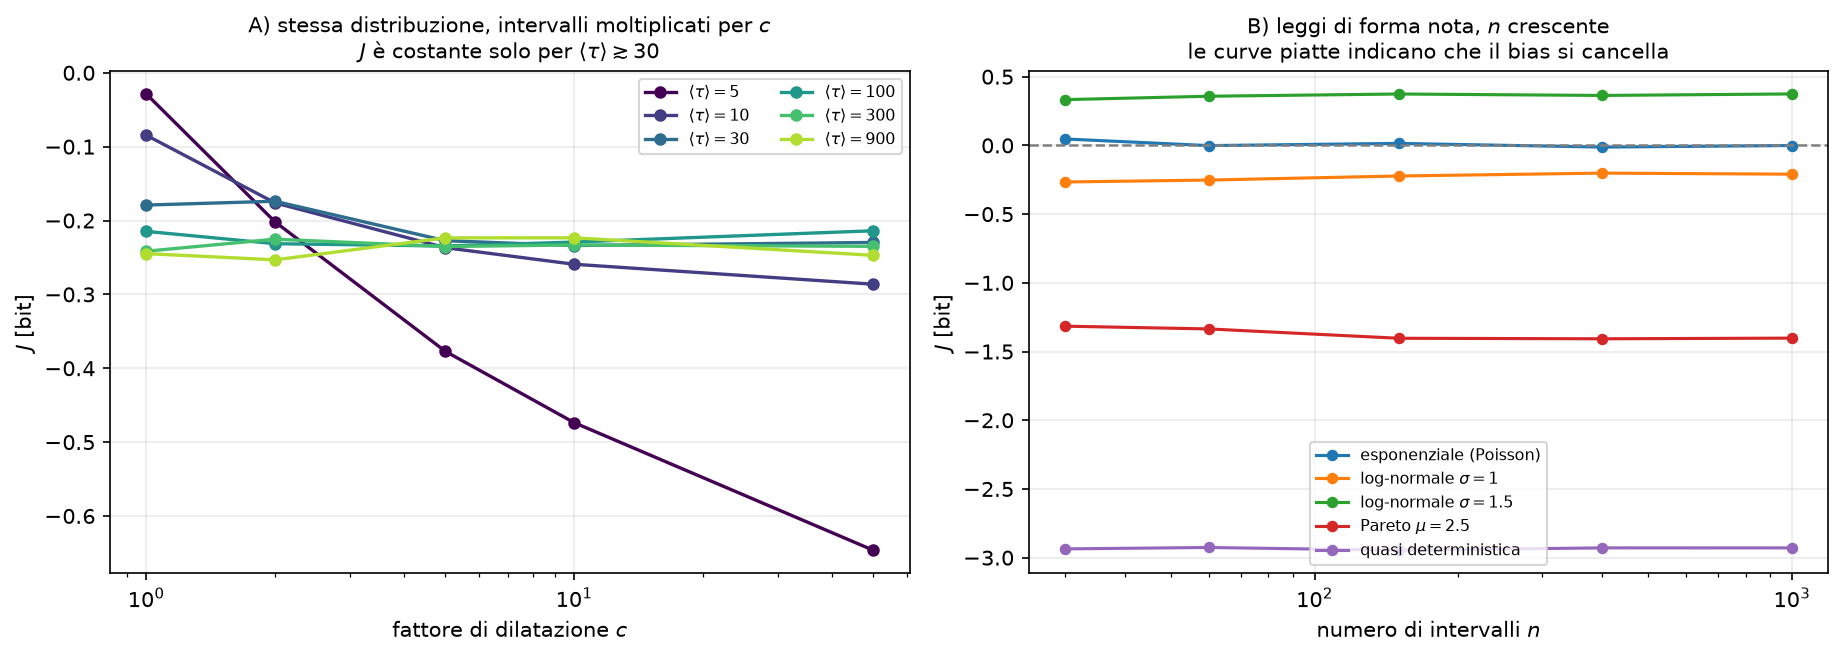
\includegraphics[width=\textwidth]{figure/cap2_invarianza_J.png}
  \caption{Limiti di validità della~\eqref{eq:entropia-intervalli}, misurati
  sullo stimatore effettivamente impiegato. A: intervalli estratti da una stessa
  legge log-normale e moltiplicati per un fattore $c$, per sei valori
  dell'intervallo medio di partenza; una curva piatta indica invarianza. Sotto
  $\langle\tau\rangle \simeq 30$ la quantizzazione agli interi la distrugge. B:
  $J$ su cinque leggi di forma nota al crescere del numero di intervalli; lo
  scostamento fra gli estremi quantifica il bias che la sottrazione del termine
  poissoniano non elimina.}
  \label{fig:invarianza-J}
\end{figure}

Valori positivi di $J$ indicano intervalli distribuiti in modo più irregolare di
un processo di Poisson, valori negativi una regolarità superiore a quella del
caso. La quantità non compare in nessuno dei lavori di riferimento ed è
introdotta qui; il §\ref{sec:entropia-intervalli} ne verifica la stabilità
rispetto alla lunghezza di analisi e la impiega per neutralizzare l'effetto
appena descritto.


% ---------------------------------------------------------------------
\section{Entropia e compressione}
\label{sec:entropia}

Il concetto di disordine di un testo e la nozione di entropia sono già stati
introdotti nel Capitolo~\ref{cap:introduzione}. Trattandosi di un concetto
centrale per questo lavoro, in questa sezione viene definito in modo formale e
ne viene esplicitato il legame con gli algoritmi di compressione, che è lo
strumento con cui l'entropia verrà effettivamente stimata sui testi.

% ---------------------------------------------------------------------
\subsection{Entropia e predicibilità}
\label{sec:entropia-def}

Si consideri una sorgente che emette simboli da un alfabeto finito
$\mathcal{X}$. Per una singola variabile aleatoria $X$ che assume il valore
$x \in \mathcal{X}$ con probabilità $p(x)$, l'entropia di
Shannon~\cite{shannon1948} è
\begin{equation}
  H(X) \;=\; -\sum_{x \in \mathcal{X}} p(x) \log_2 p(x),
  \label{eq:H-singola}
\end{equation}
espressa in bit, e misura l'incertezza media sull'esito dell'estrazione.

I simboli di un testo non sono però indipendenti, e l'entropia di una singola
lettera non descrive la sorgente: sapere che in inglese la lettera più frequente
è \emph{e} dice poco, mentre sapere che dopo \emph{th} segue quasi sempre
\emph{e} dice molto. Occorre quindi considerare blocchi di simboli. Detta
$H(X_1,\dots,X_n)$ l'entropia congiunta di un blocco di lunghezza $n$, definita
dalla~\eqref{eq:H-singola} applicata alla distribuzione congiunta dei blocchi, si
definisce il tasso di entropia della sorgente come
\begin{equation}
  h \;=\; \lim_{n\to\infty} \frac{H(X_1,\dots,X_n)}{n} .
  \label{eq:tasso-entropia}
\end{equation}
Il limite esiste per sorgenti stazionarie ed ergodiche~\cite{cover2006} e
quantifica l'incertezza media per simbolo una volta tenuto conto di tutte le
dipendenze, comprese quelle a lunga distanza. È questa, e non
la~\eqref{eq:H-singola}, la quantità pertinente per un testo.

Il teorema della codifica di sorgente~\cite{cover2006} lega $h$ alla
comprimibilità: il tasso di entropia è un limite inferiore alla lunghezza media
per simbolo di qualunque codifica senza perdita. Stimare l'entropia di un testo
e stimarne la comprimibilità sono quindi, entro le approssimazioni del caso, lo
stesso problema.

Il legame si comprende in modo intuitivo tornando ai casi limite della
Tabella~\ref{tab:tre-regimi}. Un algoritmo di compressione senza perdita opera
sostituendo alle porzioni di testo che si ripetono un riferimento
all'occorrenza precedente, più breve del testo che rimpiazza. Nel testo monotono
il medesimo gruppo di parole ricorre per l'intera lunghezza del documento: dopo
la prima occorrenza tutto il resto è un riferimento, il file compresso è
minuscolo e il tasso di entropia è prossimo a zero, perché il simbolo successivo
è quasi sempre determinato da quelli che lo precedono. Nella sequenza casuale,
al contrario, nessuna porzione si ripete: non esiste nulla cui fare riferimento,
il compressore non guadagna nulla e il tasso di entropia è massimo, perché ogni
simbolo è imprevedibile a partire dai precedenti. Il linguaggio naturale si
colloca fra i due estremi, e la quantità di compressione che ammette è una
misura diretta di quanta struttura possiede.

\paragraph{Stimatori di Lempel--Ziv.}
La stima diretta di $h$ dalla~\eqref{eq:tasso-entropia} per conteggio di blocchi
è impraticabile: il numero di blocchi distinti di lunghezza $n$ cresce
esponenzialmente con $n$, e la dimensione campionaria necessaria a stimarne le
probabilità cresce di conseguenza. Nessun testo reale è abbastanza lungo.

Si ricorre allora agli stimatori della famiglia Lempel--Ziv~\cite{ziv1977},
che aggirano il problema misurando le ripetizioni invece delle probabilità.
L'idea è la seguente: si scorre la successione e, a ogni posizione $i$, si cerca
la più lunga sottostringa che inizi in $i$ e sia già comparsa in precedenza,
detta $\Lambda_i$ la sua lunghezza. In un testo molto ripetitivo i match sono
lunghi, in un testo casuale sono corti. Si dimostra che, per una sorgente
stazionaria ed ergodica, la lunghezza media di tali match cresce come il
logaritmo della finestra esplorata e che
\begin{equation}
  h \;=\; \lim_{n\to\infty}
  \left\langle \frac{\log_2 n}{\Lambda_i} \right\rangle ,
  \label{eq:lz-entropia}
\end{equation}
dove la media è presa sulle posizioni $i$. La~\eqref{eq:lz-entropia} converge
assai più rapidamente del conteggio di blocchi e mantiene buone proprietà anche
in presenza di correlazioni a lungo raggio, che è la ragione per cui viene
adottata qui: le sorgenti considerate in questa tesi hanno, per costruzione,
memoria lunga.

% ---------------------------------------------------------------------
\subsection{Stima della cross-entropia e della divergenza}
\label{sec:crossparsing}

Le quantità introdotte finora descrivono un testo singolo. Per confrontare due
testi occorre la cross-entropia, che misura il costo di codificare un testo
usando la statistica di un altro.

L'algoritmo di cross-parsing di Ziv e Merhav~\cite{ziv1993} estende
la~\eqref{eq:lz-entropia} a due successioni. Data la successione $x$ da
misurare e la successione di riferimento $y$, si scorre $x$ da sinistra a destra
e la si decompone in frasi successive, dove ogni frase è la più lunga
sottostringa che, a partire dalla posizione corrente, compaia da qualche parte
in $y$; raggiunto il punto in cui il match si interrompe, si chiude la frase e
se ne apre una nuova. Il numero di frasi così ottenute viene indicato con
$c(x|y)$ ed è la quantità che misura la somiglianza fra i due testi: se $x$ e
$y$ provengono dalla stessa sorgente, le frasi sono lunghe e poche; se
provengono da sorgenti diverse, i match si interrompono presto e le frasi sono
molte. La stima della cross-entropia è
\begin{equation}
  h(x \,|\, y) \;=\; \frac{c(x|y)\,\log_2 |y|}{|x|},
  \label{eq:crossparsing}
\end{equation}
espressa in bit per simbolo, dove $|x|$ e $|y|$ sono le lunghezze delle due
successioni.

La divergenza di Kullback--Leibler è lo strumento con cui si quantifica quanto
due distribuzioni di probabilità differiscano fra loro. Date due distribuzioni
$P$ e $Q$ sullo stesso alfabeto, essa è definita come
\begin{equation}
  D(P\|Q) \;=\; \sum_{x} P(x) \log_2 \frac{P(x)}{Q(x)}
  \;=\; H_P(Q) - H(P),
  \label{eq:kl-def}
\end{equation}
dove $H_P(Q)$ è la cross-entropia fra le due distribuzioni. La~\eqref{eq:kl-def}
si interpreta come il numero medio di bit sprecati per simbolo codificando una
sorgente $P$ con un codice ottimizzato per $Q$: vale zero se e solo se
$P = Q$ ed è positiva altrimenti.

In termini di successioni, la~\eqref{eq:kl-def} si stima come differenza fra due
cross-entropie: dividendo $x$ in due metà $x_1$ e $x_2$ e prendendo da $y$ un
prefisso $y_1$ della stessa lunghezza di $x_1$, si pone
\begin{equation}
  D(x \,\|\, y) \;=\; h(x_2 \,|\, y_1) \;-\; h(x_2 \,|\, x_1) .
  \label{eq:kl}
\end{equation}
La seconda metà di $x$ viene cioè codificata due volte, una volta usando come
riferimento un testo estraneo e una volta usando la prima metà di $x$ stesso, e
si misura quanto costa in più la prima operazione.

L'appaiamento delle lunghezze dei due riferimenti non è un dettaglio.
La~\eqref{eq:crossparsing} dipende dalla lunghezza del riferimento, poiché un
riferimento più lungo contiene più sottostringhe e produce una cross-entropia
minore a parità di sorgente. Se i due termini della~\eqref{eq:kl} usassero
riferimenti di lunghezza diversa, la differenza conterrebbe un termine spurio
che può superare in modulo il segnale da misurare e produrre stime negative,
impossibili per la~\eqref{eq:kl-def}. Con $|y_1| = |x_1|$ il termine spurio si
cancella, e la costruzione soddisfa la proprietà verificabile $D(x\|x) = 0$
esattamente, impiegata nei capitoli sperimentali come test dello stimatore.

Poiché la~\eqref{eq:kl} non è simmetrica, mentre per confrontare due corpora
serve una quantità che non dipenda da quale dei due venga posto come
riferimento, seguendo~\cite{lippi2019} viene adottata la divergenza
simmetrizzata
\begin{equation}
  D_s(x,y) \;=\; \tfrac{1}{2}\bigl[D(x\|y) + D(y\|x)\bigr].
  \label{eq:kl-sym}
\end{equation}

% ---------------------------------------------------------------------
\subsection{Misure basate su compressione}
\label{sec:compressione}

Le stime della sottosezione precedente usano la compressione come strumento
teorico, attraverso il conteggio delle frasi. Un secondo gruppo di misure,
introdotto in questo contesto da Hadad et al.~\cite{hadad2026}, impiega invece
direttamente un compressore reale come sonda della regolarità strutturale, senza
passare per una stima di entropia.

Detta $C(x)$ la dimensione in byte del testo $x$ dopo la compressione, si
definisce il rapporto di compressione
\begin{equation}
  R_{\mathrm{gzip}}(x) \;=\; \frac{C(x)}{|x|},
  \label{eq:cratio}
\end{equation}
tanto minore quanto più il testo è regolare. Il pedice ricorda l'algoritmo
impiegato e distingue la quantità dal descrittore $R$ della~\eqref{eq:R}.

Da esso derivano la compressione condizionata
$\bigl(C(x+y) - C(x)\bigr)/|y|$, dove $x+y$ indica la concatenazione, che stima
il costo incrementale di codificare la seconda metà di un documento dopo aver
già codificato la prima e misura quindi quanto la seconda metà sia prevedibile
a partire dalla prima; e la distanza normalizzata di compressione~\cite{li2004}
\begin{equation}
  \mathrm{NCD}(x,y) \;=\;
  \frac{C(xy) - \min\{C(x),C(y)\}}{\max\{C(x),C(y)\}} .
  \label{eq:ncd}
\end{equation}
Applicata fra un testo e una sua permutazione, la~\eqref{eq:ncd} misura quanta
parte della comprimibilità dipenda dall'ordine delle parole e non dalla sola
composizione lessicale: è quindi l'analogo, in chiave di compressione, del
confronto fra i pannelli della Figura~\ref{fig:barcode}.


% ---------------------------------------------------------------------
\section{Token ed embedding}
\label{sec:token}

Nel §\ref{sec:scala} si è assunta la parola come unità fondamentale del testo,
in quanto più piccola porzione dotata di significato autonomo per un lettore
umano. Questa scelta non vale più per gli algoritmi di generazione automatica
del testo e, in particolare, per i modelli linguistici di grandi dimensioni.

Si riprenda la frase già usata come esempio,
\emph{Se pensi di comprendere la meccanica quantistica, non comprendi la
meccanica quantistica.} Per un lettore umano essa si scompone come nella
Figura~\ref{fig:scomp-parole}: dodici parole più la punteggiatura, ciascuna
delle quali ha un significato che si può cercare in un dizionario.

\begin{figure}[htbp]
  \centering
  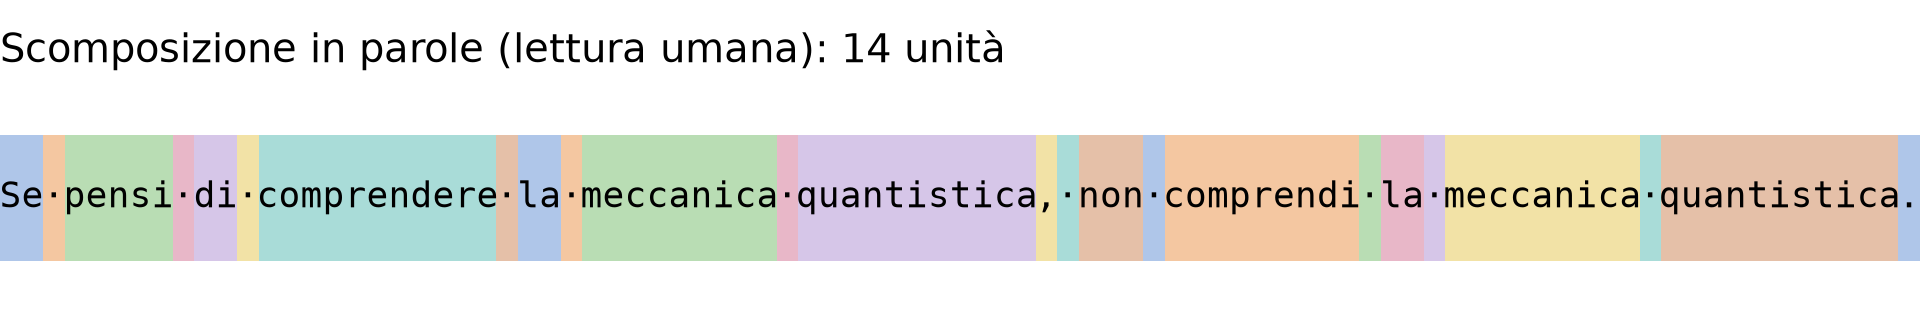
\includegraphics[width=\textwidth]{figure/cap2_scomposizione_parole.png}
  \caption{Scomposizione in parole. Ogni blocco è un'unità dotata di
  significato autonomo; il punto mediano segnala gli spazi.}
  \label{fig:scomp-parole}
\end{figure}

Per un modello linguistico la stessa frase si scompone invece come nella
Figura~\ref{fig:scomp-token}.

\begin{figure}[htbp]
  \centering
  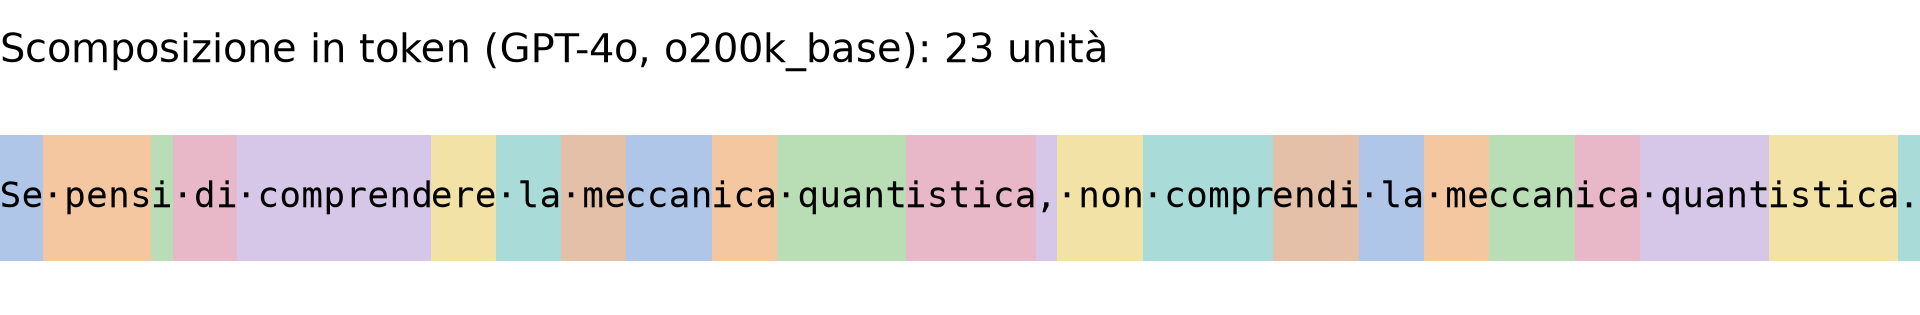
\includegraphics[width=\textwidth]{figure/cap2_scomposizione_token.png}
  \caption{Scomposizione in token della stessa frase, ottenuta con il
  tokenizzatore \texttt{o200k\_base} impiegato da GPT-4o. Le unità sono
  ventitré, non coincidono con le parole e in generale non hanno significato
  autonomo.}
  \label{fig:scomp-token}
\end{figure}

La frase non è divisa né in lettere né in parole, ma in gruppi di lettere
chiamati \emph{token}. Alcuni token coincidono con parole intere
(\texttt{·la}, \texttt{·non}), altri sono frammenti privi di significato
(\texttt{ccan}, \texttt{istica}). Si osservi in particolare la coppia
\emph{comprendere} e \emph{comprendi}: la prima si scompone in
\texttt{·comprend} e \texttt{ere}, la seconda in \texttt{·compr} e
\texttt{endi}. Due forme della stessa radice vengono dunque tagliate in punti
diversi, e il modello non riceve alcuna indicazione esplicita del fatto che
condividano la radice. Lo spazio, inoltre, non separa i token ma vi è
incorporato: la maggior parte dei token inizia con uno spazio, e la
segmentazione del testo in unità precede logicamente qualunque nozione di
parola.

La conversione avviene tramite un algoritmo detto \emph{tokenizzatore}, che
traduce un testo scritto in una qualsiasi lingua e in un qualsiasi alfabeto in
una sequenza di token estratti da un dizionario ampio ma finito, costruito una
volta per tutte a partire da un grande corpus. I dizionari dei tokenizzatori
più diffusi hanno dimensioni dell'ordine di $10^5$ elementi: quello di GPT-4o,
\texttt{o200k\_base}, ne conta \num{200019}; \texttt{cl100k\_base}, impiegato
come unità di analisi nei capitoli sperimentali per le ragioni discusse nel
Capitolo~\ref{cap:metodi}, ne conta \num{100277}; i modelli Qwen2.5 analizzati
in questa tesi ne condividono uno di circa \num{151000} voci. Poiché il
dizionario è finito ma le lingue possibili sono molte, i testi nelle lingue
meno rappresentate nel corpus di costruzione vengono frammentati in un numero
di token assai maggiore rispetto all'inglese.

Proprio come le parole per gli esseri umani, per un modello linguistico sono i
token a trasportare significato. Il significato non è però un'etichetta
associata al token, bensì una posizione: tramite un'operazione detta
\emph{embedding} ogni token viene mappato in un vettore di uno spazio a molte
dimensioni, e la geometria di quello spazio codifica le relazioni fra i token.
Vettori vicini corrispondono a token che compaiono in contesti simili, e
direzioni ricorrenti nello spazio corrispondono a relazioni ricorrenti nel
linguaggio.

La Figura~\ref{fig:embedding} mostra la proprietà su un caso concreto. I vettori
di trenta parole inglesi, appartenenti a cinque famiglie semantiche, sono
proiettati sulle prime due componenti principali dello spazio: le parole di
ciascuna famiglia si dispongono in gruppi distinti, benché la costruzione dei
vettori non abbia mai fatto uso di alcuna classificazione semantica, ma soltanto
delle co-occorrenze osservate in un corpus.

\begin{figure}[htbp]
  \centering
  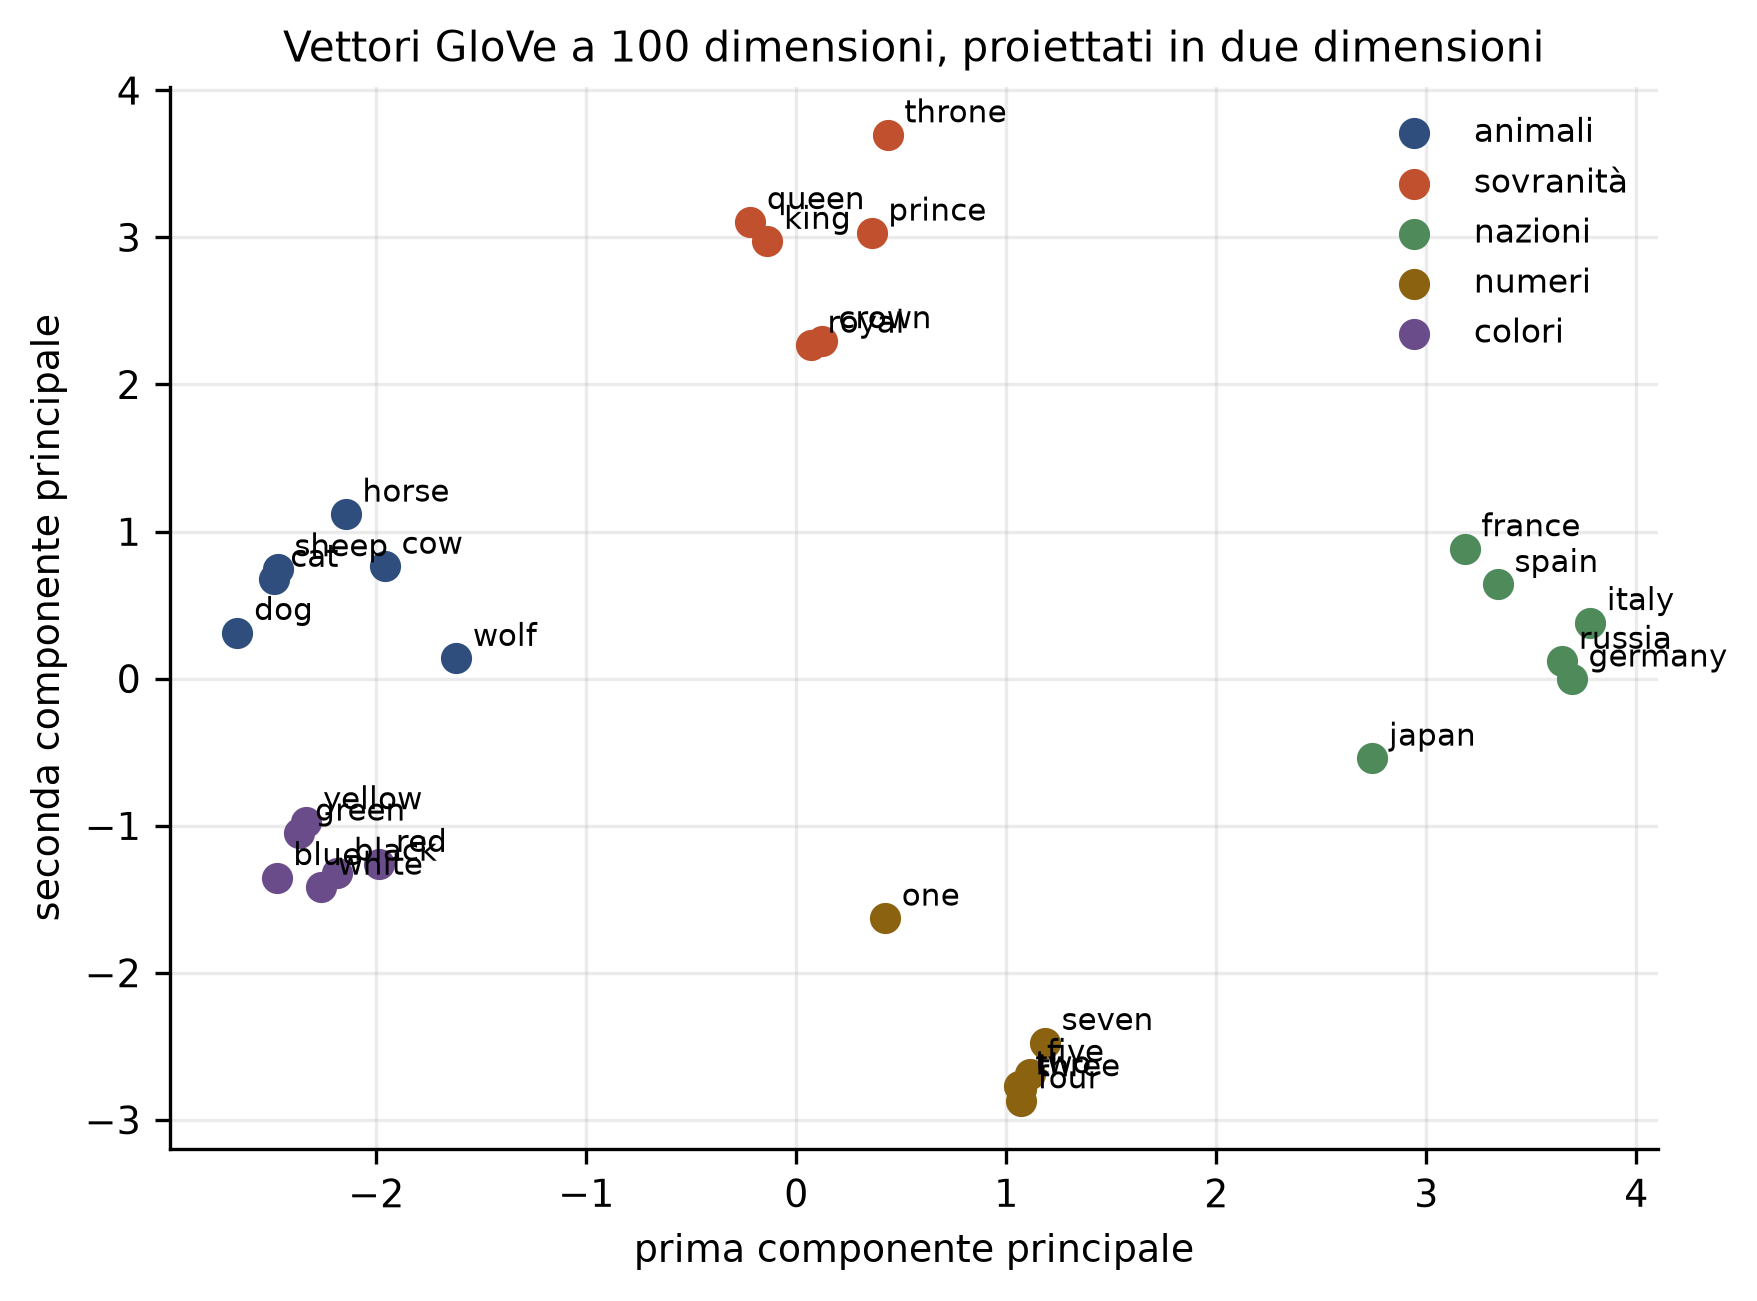
\includegraphics[width=0.82\textwidth]{figure/cap2_embedding_2d.png}
  \caption{Trenta parole inglesi rappresentate dai rispettivi vettori GloVe a
  100 dimensioni, proiettati sulle prime due componenti principali. Le cinque
  famiglie semantiche formano gruppi separati senza che alcuna informazione
  semantica sia stata fornita all'algoritmo. La proiezione conserva soltanto una
  parte della struttura, poiché riduce cento dimensioni a due: la vicinanza
  visibile in figura è una condizione sufficiente, non necessaria, alla
  vicinanza nello spazio originario.}
  \label{fig:embedding}
\end{figure}

I due spazi vettoriali che compaiono in questo lavoro hanno natura diversa. Ogni modello linguistico possiede una propria matrice di embedding,
appresa durante l'addestramento insieme a tutti gli altri parametri, e i cui
vettori non sono direttamente confrontabili fra modelli diversi: fra i modelli
analizzati in questa tesi la dimensione di tale spazio passa da 1536 per il
modello da 1.5 miliardi di parametri a 5120 per quello da 14 miliardi. Gli embedding impiegati nelle analisi di
questa tesi sono invece vettori GloVe a 100 dimensioni, pre-addestrati su un
corpus esterno e identici per tutti i testi esaminati: la scelta è dettata dalla
necessità di misurare i testi generati da modelli diversi con lo stesso metro, e
segue l'impostazione di~\cite{mikhaylovskiy2025states}. Nel
§\ref{sec:traiettoria} tali vettori verranno usati per trasformare un testo in
una traiettoria nello spazio semantico e studiarne l'autocorrelazione.


% ---------------------------------------------------------------------
\section{Generazione autoregressiva e temperatura}
\label{sec:temperatura}

Un modello linguistico autoregressivo, data una sequenza di token $t_{1:m}$,
sceglie il token successivo estraendolo da una distribuzione di probabilità che
dipende dalla sequenza stessa. La probabilità dell'intera sequenza si
decompone per mezzo della regola della catena,
\begin{equation}
  P(t_{1:m}) \;=\; \prod_{k=1}^{m} P(t_k \mid t_{1:k-1}),
  \label{eq:autoregressivo}
\end{equation}
e il modello è addestrato ad approssimare i singoli fattori
$P(t_k \mid t_{1:k-1})$, cioè a prevedere ogni token a partire da tutti quelli
che lo precedono. La generazione consiste nell'applicare ripetutamente questa
previsione, aggiungendo di volta in volta il token estratto alla sequenza che
condiziona l'estrazione successiva.

\paragraph{Origine della distribuzione condizionata.}
Il modo in cui il modello costruisce $P(t_k \mid t_{1:k-1})$ è ciò che
distingue le architetture moderne da quelle precedenti, ed è rilevante per
questo lavoro. I modelli oggi in uso si basano sull'architettura
\emph{transformer}~\cite{vaswani2017}, il cui elemento caratteristico è il
meccanismo di \emph{attenzione}. In esso ogni posizione della sequenza calcola
un peso per ciascuna delle posizioni precedenti e costruisce la propria
rappresentazione come combinazione pesata di quelle: il token in posizione $k$
può quindi attingere direttamente a qualunque token precedente, per lontano che
sia, senza che l'informazione debba propagarsi attraverso le posizioni
intermedie.

È una differenza sostanziale rispetto ai modelli ricorrenti, in cui
l'informazione proveniente da una posizione lontana deve attraversare tutte
quelle interposte e si degrada di conseguenza. Nel transformer il cammino fra
due posizioni qualsiasi ha lunghezza costante, e questo rende l'architettura in
linea di principio capace di rappresentare dipendenze fra porzioni di testo
molto distanti fra loro. È il meccanismo che, negli attuali modelli, potrebbe
dare origine alle correlazioni a lungo raggio descritte nel §\ref{sec:lrc}, e
una delle ragioni per cui ha senso cercarle nel testo generato. La capacità di
rappresentare tali dipendenze non implica però che il modello le riproduca
effettivamente, e l'attenzione opera comunque entro una finestra di contesto
finita: stabilire se le correlazioni siano presenti nel
testo prodotto resta una questione empirica, ed è precisamente quella affrontata
nei capitoli sperimentali.

\paragraph{Temperatura.}
Il modello non produce direttamente probabilità, ma valori reali detti
\emph{logit}, indicati con $u_1,\dots,u_{|\mathcal{L}|}$, uno per ciascun
elemento del dizionario $\mathcal{L}$. Essi vengono convertiti in distribuzione
di probabilità da una funzione softmax riscalata da un parametro
$T$~\cite{ackley1985}:
\begin{equation}
  p(t = \mathcal{L}_l \mid t_{1:i-1}) \;=\;
  \frac{\exp(u_l / T)}{\sum_{l'} \exp(u_{l'} / T)} .
  \label{eq:softmax}
\end{equation}

Il parametro $T$ prende il nome di temperatura, e la denominazione non è una
semplice analogia. Ponendo $E_l = -u_l$, la~\eqref{eq:softmax} coincide con la
distribuzione di Boltzmann $p_l \propto e^{-E_l/T}$ di un sistema a
$|\mathcal{L}|$ stati in equilibrio termico alla temperatura $T$. Questa
identificazione è ciò che giustifica la ricerca, nel testo generato, dei
fenomeni caratteristici dei sistemi termodinamici, e in particolare delle
transizioni di fase discusse nel §\ref{sec:fasi}.

I due limiti sono immediati. Per $T\to0$ la distribuzione si concentra sul token
di logit massimo e la generazione diventa deterministica; per $T\to\infty$ tende
alla distribuzione uniforme sull'intero dizionario, indipendentemente dal
contesto. Fra i due estremi, valori $T<1$ concentrano la massa di probabilità
sugli eventi più probabili, mentre valori $T>1$ la ridistribuiscono verso quelli
meno probabili. La temperatura non modifica dunque ciò che il modello ha
appreso, ma soltanto quanto fedelmente la generazione segue la distribuzione
appresa.

Nella pratica corrente la generazione impiega anche il troncamento della
distribuzione, nelle varianti top-$k$~\cite{fan2018} e
top-$p$~\cite{holtzman2020}, e penalità che scoraggiano la ripetizione. Tutti
questi meccanismi agiscono sulla stessa distribuzione e introducono un secondo
parametro d'ordine, rendendo impossibile attribuire alla sola temperatura il
comportamento osservato. Per questa ragione, e coerentemente con la scelta
esplicita di~\cite{mikhaylovskiy2025zipf}, i dati analizzati in questa tesi sono
stati generati impiegando il solo campionamento per temperatura.


% ---------------------------------------------------------------------
\section{Fasi e stato critico}
\label{sec:fasi}

Una fase di un sistema fisico è uno stato, tipicamente di equilibrio, dotato di
proprietà macroscopiche caratteristiche e stabile in una regione dello spazio
dei parametri; alla frontiera di tali regioni avviene una transizione di fase.
Secondo la classificazione di Ehrenfest~\cite{ehrenfest1933} una transizione di
ordine $n$ è una discontinuità nella derivata $n$-esima dell'energia libera.

Applicare alla lettera questa classificazione al testo generato non è però
possibile. Il sistema considerato non ha un'energia libera di cui prendere
derivate, non è in equilibrio con alcun bagno termico e
non possiede un limite termodinamico, poiché il numero di token di un documento
resta finito. Ciò che rende legittimo il linguaggio delle fasi è la
corrispondenza stabilita nel §\ref{sec:temperatura}: la~\eqref{eq:softmax}
coincide con una distribuzione di Boltzmann in cui i logit giocano il ruolo di
energie e il parametro di campionamento quello di temperatura. La distribuzione
condizionata da cui ogni token viene estratto è dunque, letteralmente, una
distribuzione di Gibbs, e $T$ ne è la temperatura. Quello che resta analogia, e
non identità, è il passaggio dal singolo token al documento: nulla garantisce
che le proprietà collettive di una sequenza generata token per token si
comportino come le proprietà macroscopiche di un sistema all'equilibrio. Il
vocabolario di Ehrenfest viene perciò impiegato in senso descrittivo, per
nominare regioni di comportamento qualitativamente diverso separate da
variazioni rapide, e non per rivendicare una transizione di fase in senso
termodinamico.

Ciò che rende il concetto utile è il comportamento nel punto critico che
separa due fasi: là le correlazioni decadono a legge di potenza e la loro
portata diverge, e molte grandezze osservabili esibiscono lo stesso andamento.
Il criterio inverso, per cui dove compare una legge di potenza si sospetta uno
stato critico, va maneggiato con prudenza, perché distribuzioni a legge di
potenza si generano in molti modi che con la criticità non hanno rapporto, dal
semplice prodotto di variabili aleatorie ai processi di preferential
attachment. Preso da solo, l'andamento a legge di potenza di una quantità non
dimostra nulla. Acquista forza quando più osservabili indipendenti cambiano
regime allo stesso valore del parametro di controllo, ed è in questa forma che
viene impiegato nel §\ref{sec:tstar}: non la legge di potenza di una misura,
ma la convergenza di criteri costruiti per scopi diversi.

Il quadro è stato applicato ai modelli linguistici in~\cite{nakaishi2024}, dove
la temperatura di campionamento separa una fase a bassa temperatura,
caratterizzata da strutture ripetitive, da una ad alta temperatura in cui il
testo è incomprensibile. La tesi sostenuta in quel lavoro è che il linguaggio
naturale si collochi \emph{sul} punto critico fra le due: nello spazio dei
processi stocastici che generano successioni di simboli, il processo
corrispondente a una lingua naturale giacerebbe sulla superficie critica che
separa le due regioni, e un modello addestrato su quella lingua definisce una
famiglia di processi che quella superficie attraversa al variare di $T$. Il
risultato è verificato su modelli da 160 milioni a 2.8 miliardi di parametri, su
sei lingue e su due diverse mappature del testo in successione numerica, il che
ne stabilisce l'indipendenza dalla scala e dalla lingua.

Questa congettura è il punto di contatto più stretto fra il presente lavoro e la
letteratura di fisica statistica sull'argomento, e il
Capitolo~\ref{cap:risultati1} ne fornisce una verifica indipendente: se il
linguaggio naturale è critico, allora la temperatura alla quale il testo
generato somiglia di più a quello umano deve coincidere con quella alla quale il
modello attraversa la transizione, e criteri che misurano proprietà diverse
devono indicarla concordemente.


% ---------------------------------------------------------------------
\subsection{La traiettoria di embedding}
\label{sec:traiettoria}

Il §\ref{sec:token} ha introdotto i vettori di embedding come rappresentazione
del significato. Applicandoli a un testo si ottiene un oggetto geometrico: detta
$(p_1,\dots,p_M)$ la successione delle parole del documento e $v(\cdot)$ la
mappa che associa a una parola il proprio vettore, si pone
\begin{equation}
  \mathbf{m}_i \;=\;
  \begin{cases}
    v(p_i) - \bar{v} & \text{se $p_i$ ha un vettore},\\[2pt]
    \mathbf{0}       & \text{altrimenti},
  \end{cases}
  \label{eq:traiettoria}
\end{equation}
dove $\bar{v}$ è la media dei vettori delle sole parole che ne possiedono uno.
La successione $(\mathbf{m}_1,\dots,\mathbf{m}_M)$ è la traiettoria del testo
nello spazio degli embedding: ogni parola è un punto, e leggere il documento
dall'inizio alla fine equivale a percorrere quella traiettoria.

Due dettagli della~\eqref{eq:traiettoria} incidono sui risultati. Il primo è la
centratura: sottrarre $\bar{v}$ elimina la
direzione media del documento, che altrimenti dominerebbe ogni prodotto scalare
e renderebbe tutte le coppie di parole artificialmente simili. Il secondo è il
trattamento delle parole prive di vettore, alle quali si assegna il vettore
nullo \emph{dopo} la centratura, seguendo~\cite{mikhaylovskiy2025states}: la
posizione nella successione viene così conservata, e con essa la struttura dei
lag, ma la parola non contribuisce ad alcuna correlazione. La conseguenza è che
un testo in cui molte parole non hanno vettore produce una traiettoria fatta in
larga parte di zeri, e le misure che seguono perdono significato prima di
diventare incalcolabili: è la ragione della soglia di validità introdotta più
avanti.

Su questa successione si definisce l'autocorrelazione a distanza $\tau$ come
media della similarità coseno fra i vettori che distano $\tau$ posizioni,
\begin{equation}
  C(\tau) \;=\; \frac{1}{M-\tau} \sum_{i=1}^{M-\tau}
  \frac{\mathbf{m}_i \cdot \mathbf{m}_{i+\tau}}
       {\lVert \mathbf{m}_i \rVert \, \lVert \mathbf{m}_{i+\tau} \rVert},
  \label{eq:acf-embedding}
\end{equation}
con la convenzione che i termini in cui uno dei due vettori è nullo
contribuiscono zero. La~\eqref{eq:acf-embedding} risponde alla domanda: due
parole che distano $\tau$ posizioni tendono a essere semanticamente affini? Vale
$C(\tau) \simeq 0$ quando non c'è alcuna relazione, ed è tanto più vicina a uno
quanto più il testo, a quella distanza, torna a parlare della stessa cosa.

Poiché la~\eqref{eq:acf-embedding} resta calcolabile su qualunque successione,
serve un riferimento che dica quale ampiezza sia distinguibile dal caso. Si
adotta il rimescolamento: si permutano a caso le posizioni della traiettoria, si
ricalcola $C(\tau)$ e si prende il massimo del suo modulo. Il valore così
ottenuto è il livello di rumore del documento, ed è la stessa costruzione dei
null model del §\ref{sec:null}: conserva il contenuto e distrugge l'ordine.
Un'autocorrelazione la cui ampiezza non superi quel livello non è distinguibile
da una successione di parole senza struttura.


% ---------------------------------------------------------------------
\subsection{Le tre fasi}
\label{sec:tre-fasi}

Applicando questo linguaggio al testo generato,
in~\cite{mikhaylovskiy2025states} vengono individuate tre fasi, distinte dal
comportamento di $C(\tau)$.

A bassa temperatura il testo degenera in cicli di ripetizione: la traiettoria
ripassa periodicamente per gli stessi punti, $C(\tau)$ oscilla con periodo pari
alla lunghezza del ciclo e la sua trasformata di Fourier presenta picchi netti.
La quantità che segnala il fenomeno è quindi
\begin{equation}
  \Phi \;=\; \max_{k \ge 1} \bigl\lvert \hat{C}_k \bigr\rvert ,
  \label{eq:periodicita}
\end{equation}
dove $\hat{C}_k$ sono i coefficienti della trasformata discreta di $C(\tau)$. Il
coefficiente $k = 0$ viene escluso perché proporzionale alla media di $C(\tau)$,
cioè al livello complessivo di correlazione e non alla sua periodicità: un testo
uniformemente correlato ma non ciclico ha $\hat{C}_0$ grande e tutti gli altri
coefficienti piccoli. Questa è la fase che, per analogia con gli stati della
materia, viene detta solida. È lo stesso regime in cui, come osservato nel
§\ref{sec:ponte}, la fluttuazione della DFA satura e $\alpha_{\mathrm{DFA}}$
scende verso zero: le due misure segnalano lo stesso fenomeno da due angolazioni
diverse.

La~\eqref{eq:periodicita} si comporta come un parametro d'ordine nel senso che
assume valori grandi in una fase e piccoli nell'altra, ma non si annulla
identicamente fuori dalla fase periodica: su una successione priva di struttura
resta un valore residuo dovuto alle fluttuazioni campionarie. Il
Capitolo~\ref{cap:risultati1} riporta di conseguenza il suo crollo in termini di
ordini di grandezza e non di annullamento.

In una finestra ristretta di temperature $C(\tau)$ decade invece a legge di
potenza: è lo stato critico, quello in cui le leggi di Zipf e di Heaps
introdotte nel §\ref{sec:scala} risultano meglio soddisfatte. Ad alta
temperatura, infine, le correlazioni decadono esponenzialmente e non sussiste
struttura a lungo raggio: è la fase detta amorfa, o gassosa.

Per distinguere le ultime due fasi vengono confrontati due fit
dell'autocorrelazione, uno a legge di potenza e uno esponenziale, tramite il
rapporto dei rispettivi errori~\cite{mikhaylovskiy2023}:
\begin{equation}
  \mathrm{GAPELMAPER} \;=\;
  \frac{\mathrm{MAPE}\bigl(\text{fit a legge di potenza}\bigr)}
       {\mathrm{MAPE}\bigl(\text{fit esponenziale}\bigr)},
  \label{eq:gapelmaper}
\end{equation}
dove il MAPE è quello definito nella~\eqref{eq:mape}. Il rapporto è minore di 1
quando il fit a legge di potenza descrive i dati meglio di quello esponenziale,
e segnala quindi lo stato critico; è maggiore di 1 nella fase amorfa.

La~\eqref{eq:gapelmaper} è un rapporto fra errori di fit, e come tale resta
calcolabile anche quando l'autocorrelazione è indistinguibile dal rumore; in
quel regime, però, il suo valore è privo di contenuto informativo, perché
entrambi i fit descrivono male dati che non contengono alcun segnale.

Le tre fasi, la soglia di periodicità e la condizione di validità si compongono
nella regola seguente. Detti $\kappa$ la quota di parole del documento dotate di
un vettore, $A = \max_\tau \lvert C(\tau)\rvert$ l'ampiezza
dell'autocorrelazione e $\eta$ il livello di rumore stimato per rimescolamento,
un documento viene classificato come
%
\begin{itemize}
  \item \emph{non valutabile}, se $\kappa < \kappa_{\min}$ oppure $A \le \eta$;
  \item \emph{solido}, altrimenti, se $\Phi > \Phi_{\min}$;
  \item \emph{critico}, altrimenti, se $\mathrm{GAPELMAPER} < 1$;
  \item \emph{amorfo} in ogni altro caso.
\end{itemize}
%
L'ordine dei controlli non è indifferente. La condizione di validità viene per
prima perché le altre due misure, su un documento che non la supera, sono numeri
senza referente; la periodicità viene prima del GAPELMAPER perché
un'autocorrelazione periodica non è né una legge di potenza né un esponenziale,
e sottoporla a quel confronto restituirebbe un valore arbitrario. I due valori
di soglia sono fissati nel Capitolo~\ref{cap:risultati1}, dove ne vengono
discussi l'origine e l'effetto.

I due quadri di riferimento non coincidono del tutto.
In~\cite{nakaishi2024} le fasi sono due e ciò che le separa è un punto critico,
cioè un insieme di misura nulla nello spazio dei parametri;
in~\cite{mikhaylovskiy2025states} lo stato critico diventa invece una fase a sé,
dotata di estensione finita. La differenza non è terminologica: nel primo caso
attraversare la transizione con uno sweep a passo finito significa quasi
certamente saltare il punto critico, nel secondo significa attraversare una
regione che si può campionare. Il Capitolo~\ref{cap:risultati1} riporta i dati
pertinenti alla questione senza pretendere di risolverla.


% ---------------------------------------------------------------------
\section{Notazione}
\label{sec:notazione}

Le grandezze introdotte in questo capitolo provengono da lavori che adottano
simboli in conflitto fra loro. La Tabella~\ref{tab:notazione} raccoglie la
notazione seguita in questa tesi, che viene mantenuta senza eccezioni nei
capitoli successivi.

\begin{table}[htbp]
\centering
\small
\begin{tabular}{@{}l>{\raggedright\arraybackslash}p{8.3cm}c@{}}
\toprule
Simbolo & Grandezza & Definita in \\
\midrule
\multicolumn{3}{@{}l}{\itshape Testo e vocabolario} \\
$\mathbf{W}$, $w_t$, $N$ & sequenza di parole, parola in posizione $t$, lunghezza & \eqref{eq:sequenza} \\
$\mathcal{D}$, $\mathcal{D}(t)$ & dizionario e dizionario parziale & §\ref{sec:scala} \\
$f(r)$, $\alpha$ & frequenza della parola di rango $r$, esponente di Zipf & \eqref{eq:zipf} \\
$\gamma_H$ & esponente di Heaps & \eqref{eq:heaps} \\
$R$ & parole nuove nella seconda metà, rapportate alla prima & \eqref{eq:R} \\
MAPE & errore percentuale assoluto medio del fit & \eqref{eq:mape} \\
\addlinespace
\multicolumn{3}{@{}l}{\itshape Correlazioni} \\
$x_k$ & successione binaria generata da un osservabile & \eqref{eq:osservabile} \\
$c(s)$, $\theta$ & autocorrelazione a distanza $s$ e suo esponente di decadimento & \eqref{eq:acf-power} \\
$X(t)$, $\sigma_X^2$, $\gamma$ & conteggio, sua varianza, esponente di crescita & \eqref{eq:sigma} \\
$F(s)$, $\alpha_{\mathrm{DFA}}$ & fluttuazione detrendizzata e suo esponente & \eqref{eq:dfa-alpha} \\
\addlinespace
\multicolumn{3}{@{}l}{\itshape Intervalli e burstiness} \\
$\tau_i$, $p(\tau)$ & intervalli fra occorrenze e loro distribuzione & §\ref{sec:burst} \\
cv, $B$ & coefficiente di variazione, indice di Goh--Barabási & \eqref{eq:cv}, \eqref{eq:goh} \\
$S(0)$, $c_\tau(k)$ & spettro a frequenza nulla, autocorrelazione degli intervalli & \eqref{eq:eq4} \\
$\hat\gamma_{A1}$, $\hat\gamma_{A2}$ & esponenti misurati sui due null model & §\ref{sec:null} \\
$q$ & quota di burstiness & \eqref{eq:quota} \\
$\mu$, $\tau_c$ & esponente di coda e cut-off di $p(\tau)$ & \eqref{eq:troncata} \\
$J$ & entropia degli intervalli, riferita al processo di Poisson & \eqref{eq:entropia-intervalli} \\
\addlinespace
\multicolumn{3}{@{}l}{\itshape Entropia e compressione} \\
$H$, $h$ & entropia di Shannon, tasso di entropia & \eqref{eq:H-singola}, \eqref{eq:tasso-entropia} \\
$c(x|y)$, $h(x|y)$ & frasi del cross-parsing, cross-entropia stimata & \eqref{eq:crossparsing} \\
$D(x\|y)$, $D_s$ & divergenza di Kullback--Leibler e sua versione simmetrizzata & \eqref{eq:kl}, \eqref{eq:kl-sym} \\
$C(x)$, $R_{\mathrm{gzip}}$ & dimensione compressa e rapporto di compressione & \eqref{eq:cratio} \\
NCD & distanza normalizzata di compressione & \eqref{eq:ncd} \\
\addlinespace
\multicolumn{3}{@{}l}{\itshape Generazione e fasi} \\
$u_l$, $T$ & logit del token $l$, temperatura di campionamento & \eqref{eq:softmax} \\
$C(\tau)$ & autocorrelazione della traiettoria di embedding & \eqref{eq:acf-embedding} \\
$\Phi$ & parametro di periodicità di $C(\tau)$ & \eqref{eq:periodicita} \\
GAPELMAPER & rapporto fra gli errori dei due fit dell'autocorrelazione & \eqref{eq:gapelmaper} \\
$N_{\mathrm{eff}}$ & lunghezza comune di analisi & §\ref{sec:scelte} \\
\bottomrule
\end{tabular}
\caption{Notazione adottata in questa tesi.}
\label{tab:notazione}
\end{table}

Per tre simboli la scelta operata qui si discosta da quella di almeno una delle
fonti; la Tabella~\ref{tab:collisioni} riassume le corrispondenze.

\begin{center}
\small
\begin{tabular}{@{}lcccc@{}}
\toprule
Grandezza & Qui & \cite{mikhaylovskiy2025zipf} & \cite{lippi2019} & \cite{altmann2012} \\
\midrule
Esponente di Zipf                  & $\alpha$                & $\alpha$ & $\beta$  & --- \\
Esponente di Heaps                 & $\gamma_H$              & $\beta$  & $\nu$    & --- \\
Esponente della fluttuazione (DFA) & $\alpha_{\mathrm{DFA}}$ & ---      & $\alpha$ & --- \\
Decadimento dell'autocorrelazione  & $\theta$                & ---      & $\gamma$ & $\beta$ \\
Crescita della varianza del conteggio & $\gamma$             & ---      & ---      & $\gamma$ \\
Rapporto di compressione           & $R_{\mathrm{gzip}}$     & ---      & ---      & --- \\
\bottomrule
\end{tabular}
\captionof{table}{Corrispondenza fra la notazione adottata e quella delle fonti primarie,
limitatamente ai simboli per cui le fonti divergono. Il rapporto di compressione
è indicato con $R(x)$ in~\cite{hadad2026}, dove però $R$ non ha il significato
che assume qui.}
\label{tab:collisioni}
\end{center}

Il simbolo $\alpha$ è riservato all'esponente di Zipf, come
in~\cite{mikhaylovskiy2025zipf}, mentre l'esponente della detrended
fluctuation analysis, indicato con $\alpha$ in~\cite{lippi2019}, riceve il
pedice $\mathrm{DFA}$. L'esponente di Heaps è indicato con $\gamma_H$ anziché
con $\beta$ o $\nu$, per lasciare $\gamma$ libero per l'esponente di crescita
della varianza del conteggio, che è la convenzione di~\cite{altmann2012} e
della seconda parte sperimentale. Il decadimento dell'autocorrelazione riceve
infine il simbolo $\theta$, che nessuna delle fonti impiega, poiché entrambe
le lettere che gli sono attribuite in letteratura sono già assegnate. La
lettera $R$ resta al descrittore di~\cite{mikhaylovskiy2025zipf} e il rapporto
di compressione riceve il pedice $\mathrm{gzip}$.

Valgono inoltre le convenzioni seguenti, usate nel seguito senza ulteriore
avviso. Il circonflesso indica una quantità stimata dai dati in contrapposizione
al corrispondente valore teorico, come in $\hat\gamma$. I pedici $A1$ e $A2$
indicano i due null model del §\ref{sec:null}. Il simbolo $|\cdot|$ applicato a
un insieme ne indica la cardinalità e applicato a un testo la lunghezza, in
parole o in byte secondo il contesto. Le medie sono indicate con
$\langle\cdot\rangle$ e si intendono calcolate sull'intero documento salvo
diversa indicazione.

%  Le figure sono attese in figure/; la provenienza e in appendice_figure.tex
% =====================================================================

\chapter{Quadro teorico}
\label{cap:teoria}

In questo capitolo si introducono gli strumenti matematici con cui storicamente
si sono analizzati i testi e che, anche in questo lavoro, ricopriranno un ruolo
centrale: le leggi di scala del vocabolario, le misure di correlazione a lungo
raggio, la statistica degli intervalli fra occorrenze e le stime di entropia
ottenute per compressione.

Successivamente vengono introdotti gli elementi di base del funzionamento dei
modelli linguistici di grandi dimensioni, il linguaggio delle transizioni di
fase con cui alcuni risultati verranno interpretati, e la notazione adottata nel
resto della tesi.


% ---------------------------------------------------------------------
\section{Leggi di scala del vocabolario}
\label{sec:scala}

Come già anticipato, un testo può essere visto come una sequenza di simboli,
siano essi lettere, parole o, come si vedrà nel §\ref{sec:token}, token. La
scelta più naturale per un lettore umano è assumere come unità fondamentale la
parola, in quanto più piccola unità di testo dotata di significato autonomo.

Un testo è quindi una sequenza ordinata di parole
\begin{equation}
  \mathbf{W} \;=\; (w_1, w_2, \dots, w_N),
  \label{eq:sequenza}
\end{equation}
dove $N$ è la lunghezza del testo e l'indice $t = 1,\dots,N$ individua la
posizione di ciascuna parola. L'insieme delle parole distinte che vi compaiono
si dice dizionario e si indica con $\mathcal{D}$; si definisce inoltre il
dizionario parziale $\mathcal{D}(t)$ come l'insieme delle parole distinte
contenute nel prefisso $(w_1,\dots,w_t)$. Valgono per costruzione
$\mathcal{D}(N) = \mathcal{D}$ e $\mathcal{D}(t) \subseteq \mathcal{D}(t+1)$: il
dizionario parziale è una successione non decrescente di insiemi.

A titolo di esempio si consideri la frase
\begin{center}
\emph{Se pensi di comprendere la meccanica quantistica, non comprendi la
meccanica quantistica.}
\end{center}
Con la notazione introdotta si ha $N = 12$, $w_7 = \text{\emph{quantistica}}$ e
\begin{align}
  \mathcal{D}    &= \{\text{se, pensi, di, comprendere, la, meccanica,
                          quantistica, non, comprendi}\}, \\
  \mathcal{D}(6) &= \{\text{se, pensi, di, comprendere, la, meccanica}\} .
\end{align}
Il dizionario completo contiene nove parole distinte a fronte di dodici
occorrenze: le tre ripetizioni di \emph{la}, \emph{meccanica} e
\emph{quantistica} non lo accrescono.

Le due analisi più semplici che si possano condurre su $\mathbf{W}$ sono lo
studio delle frequenze delle singole parole e quello dell'andamento di
$|\mathcal{D}(t)|$ in funzione di $t$. Sono le analisi che hanno portato alla
formulazione delle due leggi empiriche enunciate nel seguito, dovute
rispettivamente a Zipf~\cite{zipf1949} e a Herdan~\cite{herdan1964} e
Heaps~\cite{heaps1978}.

% ---------------------------------------------------------------------
\subsection{Legge di Zipf}
\label{sec:zipf}

Si contino le occorrenze di ciascuna parola distinta e si ordinino le parole per
frequenza decrescente, associando a ognuna il proprio rango $r$: la parola di
rango 1 è la più frequente del testo, quella di rango 2 la seconda, e così via.
Detta $f(r)$ la frequenza della parola di rango $r$, si osserva empiricamente in
tutti i testi naturali che
\begin{equation}
  f(r) \;\propto\; r^{-\alpha}.
  \label{eq:zipf}
\end{equation}
La~\eqref{eq:zipf} prende il nome di legge di Zipf. In coordinate
bilogaritmiche corrisponde a una retta di pendenza $-\alpha$, ed è in tali
coordinate che viene di norma rappresentata e stimata.

La Figura~\ref{fig:zipf} riporta la relazione rango-frequenza per cinque romanzi
in cinque lingue diverse. Le curve sono approssimativamente rettilinee su circa
tre decadi di rango e hanno pendenze molto simili fra loro, nonostante le opere
differiscano per epoca, lingua e lunghezza.

\begin{figure}[htbp]
  \centering
  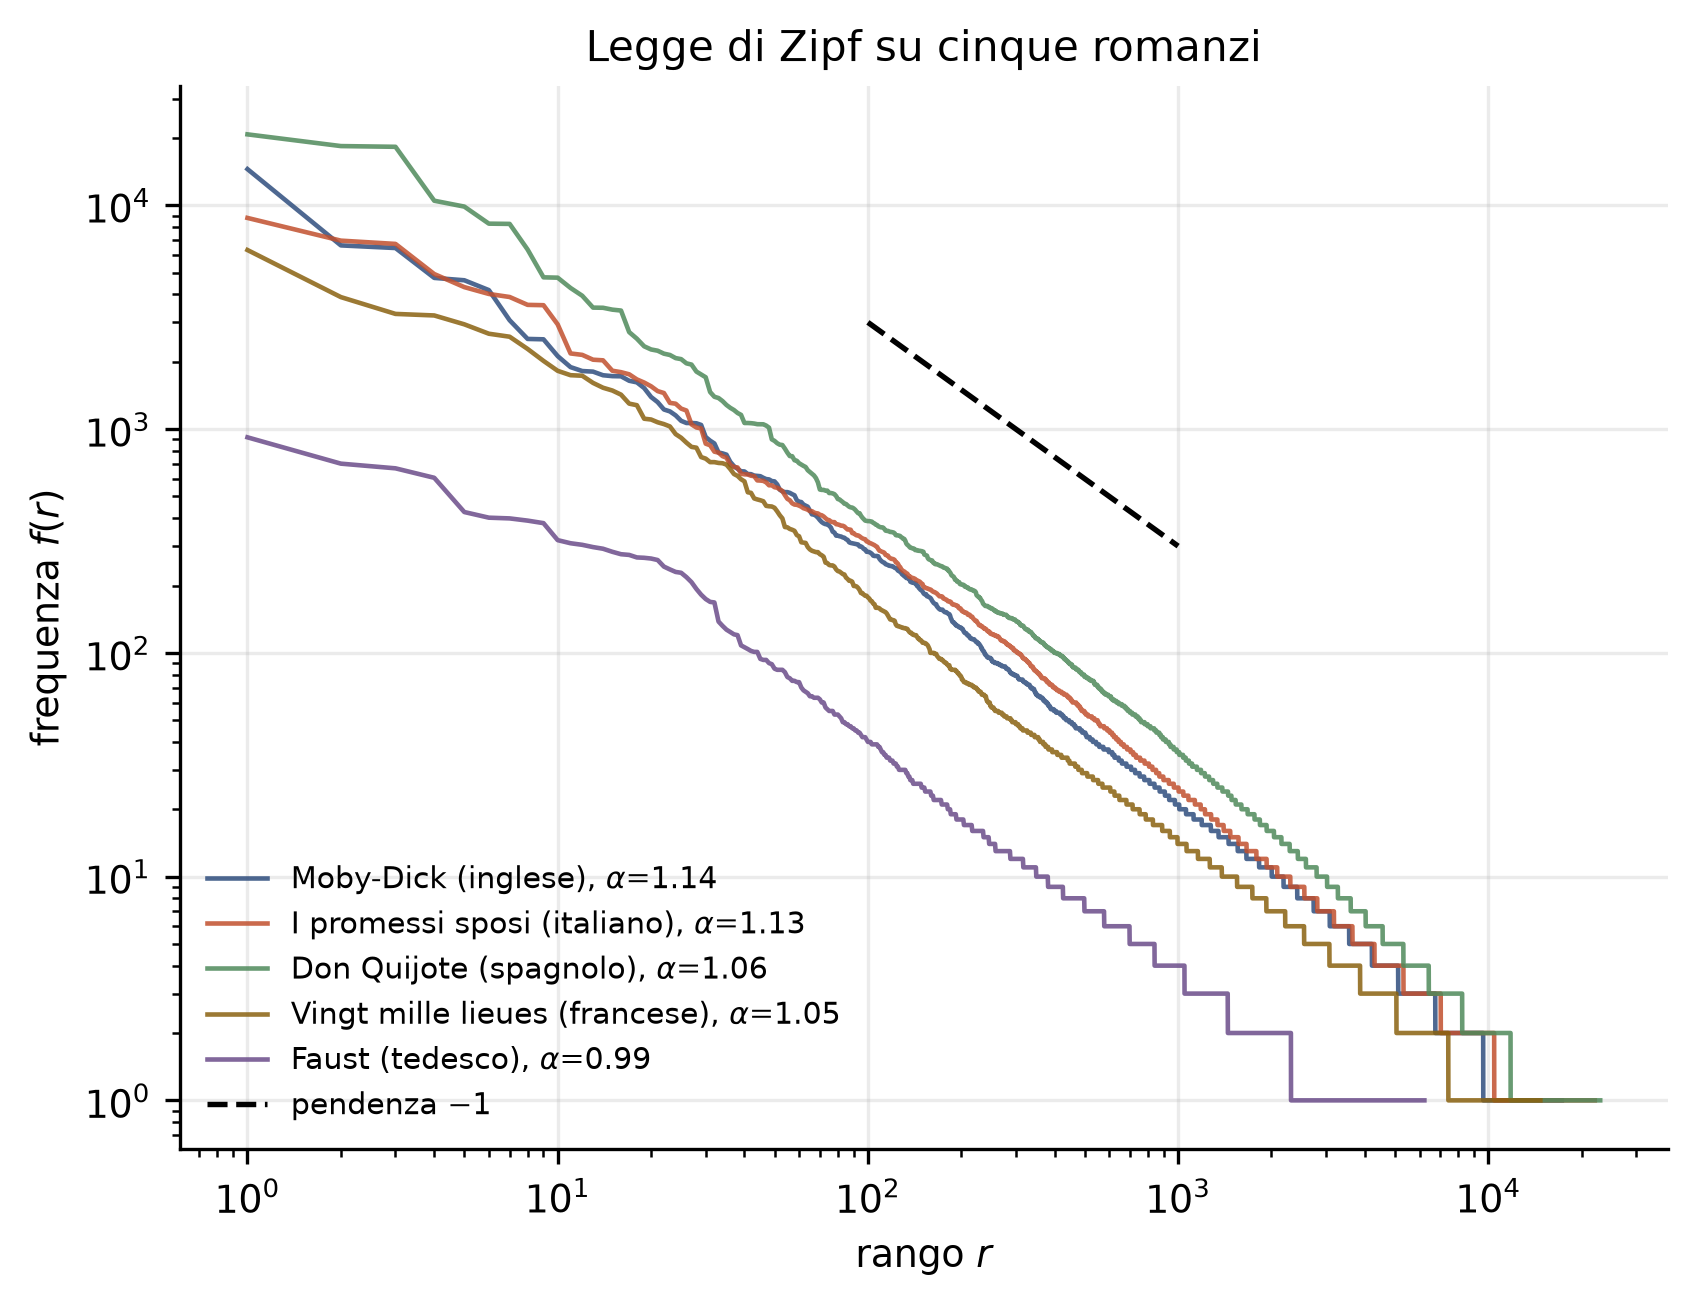
\includegraphics[width=0.82\textwidth]{figure/cap2_zipf_lingue.png}
  \caption{Relazione rango-frequenza per cinque romanzi in altrettante lingue,
  in coordinate bilogaritmiche. Gli esponenti riportati in legenda sono stimati
  per regressione ai minimi quadrati nella finestra di ranghi
  $10^2 \le r \le 10^3$, la stessa impiegata in~\cite{lippi2019}. La retta
  tratteggiata ha pendenza $-1$ ed è riportata come riferimento visivo.}
  \label{fig:zipf}
\end{figure}

Il parametro $\alpha$ risulta positivo e prossimo a 1 nella grande maggioranza
delle lingue esaminate, comprese quelle estinte e quelle costruite
artificialmente. Valori di
$\alpha$ più alti sono sintomo di un vocabolario più povero, poiché un numero
minore di parole esaurisce la maggior parte del testo; valori più bassi
segnalano al contrario una presenza più marcata di parole rare.

I valori misurati sulle cinque opere della Figura~\ref{fig:zipf} sono raccolti
nella Tabella~\ref{tab:zipf-misure}, accanto ai valori medi per lingua riportati
in~\cite{mikhaylovskiy2025zipf} su un corpus di sei opere letterarie in cinque
lingue.

\begin{table}[htbp]
\centering
\small
\begin{tabular}{@{}llrrr@{}}
\toprule
Opera & Lingua & Parole & $|\mathcal{D}|$ & $\alpha$ \\
\midrule
Moby-Dick               & inglese   & \num{219081} & \num{17258} & 1.14 \\
I promessi sposi        & italiano  & \num{239353} & \num{22040} & 1.13 \\
Don Quijote             & spagnolo  & \num{383633} & \num{22943} & 1.06 \\
Vingt mille lieues sous les mers & francese & \num{148923} & \num{14716} & 1.05 \\
Faust                   & tedesco   & \num{30959}  & \num{6221}  & 0.99 \\
\bottomrule
\end{tabular}
\caption{Esponente di Zipf misurato sulle cinque opere della
Figura~\ref{fig:zipf}, con il numero di occorrenze e la dimensione del
dizionario. La stima è condotta sui ranghi $10^2$--$10^3$.}
\label{tab:zipf-misure}
\end{table}

\begin{table}[htbp]
\centering
\small
\begin{tabular}{@{}lcccc@{}}
\toprule
& \multicolumn{2}{c}{$\alpha$ (Zipf)} & \multicolumn{2}{c}{$\gamma_H$ (Heaps)} \\
\cmidrule(lr){2-3}\cmidrule(lr){4-5}
Lingua & parole & token & parole & token \\
\midrule
inglese  & $0.952 \pm 0.072$ & $0.985 \pm 0.054$ & $0.809 \pm 0.027$ & $0.802 \pm 0.024$ \\
tedesco  & $0.959 \pm 0.054$ & $1.024 \pm 0.042$ & $0.846 \pm 0.031$ & $0.793 \pm 0.028$ \\
russo    & $1.043 \pm 0.077$ & $1.009 \pm 0.067$ & $0.916 \pm 0.049$ & $0.805 \pm 0.025$ \\
spagnolo & $0.962 \pm 0.030$ & $1.016 \pm 0.035$ & $0.842 \pm 0.025$ & $0.798 \pm 0.028$ \\
francese & $0.963 \pm 0.033$ & $0.989 \pm 0.042$ & $0.843 \pm 0.020$ & $0.801 \pm 0.018$ \\
\bottomrule
\end{tabular}
\caption{Esponenti medi per lingua riportati in~\cite{mikhaylovskiy2025zipf},
misurati su sei opere letterarie per ciascuna lingua, a livello di parola e di
token. In quel lavoro $\alpha$ è stimato sulla rappresentazione
cumulata della distribuzione anziché sulla relazione rango-frequenza; i due
stimatori coincidono soltanto nel limite $\alpha \to 1$, e i valori non vanno
quindi confrontati direttamente con quelli della
Tabella~\ref{tab:zipf-misure}.}
\label{tab:zipf-letteratura}
\end{table}

Sui testi reali si osservano deviazioni sistematiche dalla~\eqref{eq:zipf}. Su
corpora molto ampi l'esponente resta prossimo a 1 soltanto per le prime migliaia
di parole, mentre la coda continua a seguire una legge di potenza ma con
esponente maggiore~\cite{piantadosi2014}. Le parole più frequenti, inoltre,
mostrano frequenze leggermente inferiori a quelle previste: una deviazione che
Mandelbrot~\cite{mandelbrot1953} corregge introducendo un termine additivo nel
rango,
\begin{equation}
  f(r) \;\propto\; (r + c)^{-\alpha},
  \label{eq:mandelbrot}
\end{equation}
dove la costante $c > 0$ attenua la divergenza della legge di potenza ai ranghi
più bassi, spostando di fatto l'origine dell'asse dei ranghi e rendendo il fit
aderente anche nella regione delle parole più comuni.

\paragraph{Bontà del fit.}
Come si vedrà nei capitoli sperimentali, sui testi generati automaticamente
l'aderenza alla legge di potenza non è garantita. Il solo esponente non è
sufficiente a stabilirla, perché descrive la pendenza media della curva e non la
sua forma: una curva marcatamente incurvata in coordinate bilogaritmiche può
avere la stessa pendenza media di una retta, e restituire quindi un valore di
$\alpha$ del tutto ordinario pur non essendo una legge di potenza. Occorre
perciò una seconda quantità, che misuri quanto i dati si discostino dalla retta
interpolante.

Seguendo~\cite{mikhaylovskiy2025zipf}, la qualità del fit viene stimata con
l'errore percentuale assoluto medio
\begin{equation}
  \mathrm{MAPE} \;=\; \frac{1}{n}\sum_{i=1}^{n}
  \left| \frac{y_i - \hat{y}_i}{y_i} \right|,
  \label{eq:mape}
\end{equation}
dove $n$ è il numero di punti su cui è condotta la regressione, $y_i$ il valore
osservato e $\hat{y}_i$ quello previsto dalla retta interpolante in
corrispondenza dello stesso rango. Il MAPE è nullo per dati perfettamente
allineati e cresce al crescere della distanza relativa dalla retta;
essendo definito su scarti relativi, non dipende dall'unità di misura né
dall'ampiezza delle frequenze, e resta quindi confrontabile fra testi di
lunghezza diversa.

Sul corpus di testi letterari usato in~\cite{mikhaylovskiy2025zipf} il MAPE vale
in media $0.156$ con deviazione standard $0.077$. Nei capitoli sperimentali il
suo minimo in funzione della temperatura di generazione individuerà il regime in
cui il testo prodotto è più vicino a una legge di potenza.

% ---------------------------------------------------------------------
\subsection{Legge di Heaps}
\label{sec:heaps}

Studiando l'andamento di $|\mathcal{D}(t)|$ nei testi letterari emerge una
seconda regolarità, nota come legge di Heaps o, dal nome di chi la formulò per
primo~\cite{herdan1964}, di Herdan--Heaps:
\begin{equation}
  |\mathcal{D}(t)| \;\propto\; t^{\gamma_H}, \qquad \gamma_H \in [0,1] .
  \label{eq:heaps}
\end{equation}
Qui $t$ è la posizione nel testo, misurata in numero di parole,
$|\mathcal{D}(t)|$ la dimensione del dizionario parziale e $\gamma_H$
l'esponente di Heaps. I due estremi dell'intervallo corrispondono a due
comportamenti limite: $\gamma_H = 0$ descrive un dizionario che cessa di
crescere, cioè un testo che non introduce più parole nuove, mentre
$\gamma_H = 1$ descrive un dizionario che cresce proporzionalmente alla
lunghezza, cioè un testo in cui ogni parola è nuova. Poiché il dizionario non
può crescere più rapidamente del testo che lo contiene, si ha necessariamente
$|\mathcal{D}(t)| \le t$, e l'esponente non può eccedere l'unità.

La legge di Heaps quantifica dunque la capacità di un testo di rinnovare il
proprio vocabolario, ed è per questo particolarmente istruttiva se si torna alla
Tabella~\ref{tab:tre-regimi} del Capitolo~\ref{cap:introduzione}. Il primo
esempio, monotono e ripetitivo, cessa rapidamente di accrescere il dizionario;
l'ultimo, in cui i caratteri sono estratti a caso, produce quasi soltanto parole
nuove e fa crescere il dizionario senza saturare. La Figura~\ref{fig:heaps}
mostra le curve dei due casi limite accanto a quelle di tre testi letterari.

\begin{figure}[htbp]
  \centering
  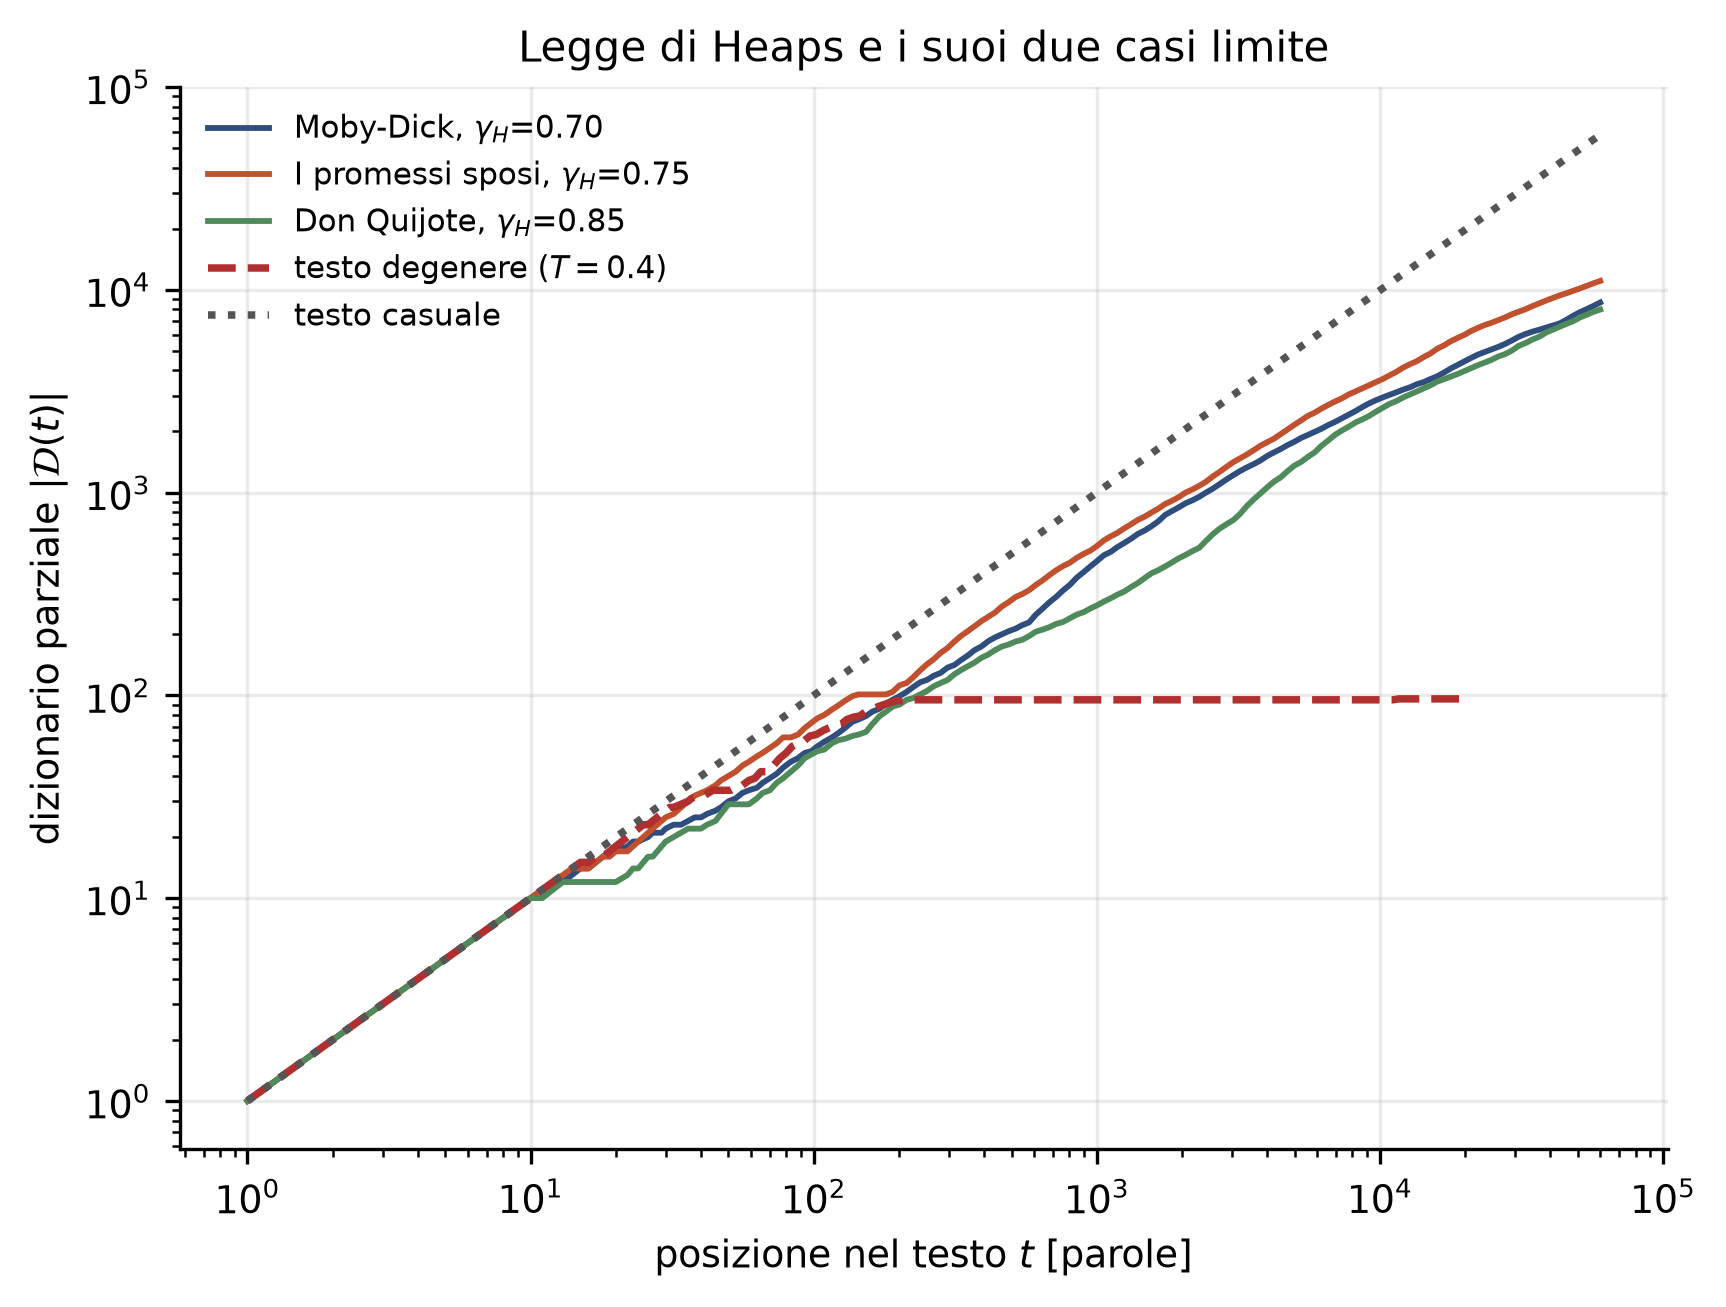
\includegraphics[width=0.82\textwidth]{figure/cap2_heaps_confronto.png}
  \caption{Crescita del dizionario parziale in coordinate bilogaritmiche. Le tre
  curve continue sono testi letterari, con esponente stimato nella regione
  $t > 1000$. La curva tratteggiata è il campione generato a $T = 0.4$ già
  riportato nella Tabella~\ref{tab:tre-regimi}: dopo circa un centinaio di
  parole entra in un ciclo di ripetizione e il dizionario si arresta. La curva
  punteggiata è una sequenza di caratteri casuali, in cui ogni parola è nuova e
  la crescita è esattamente lineare.}
  \label{fig:heaps}
\end{figure}

L'esponente stimato dipende inoltre dall'intervallo su cui viene condotta la
regressione, e quindi dalla lunghezza del testo analizzato. La
Figura~\ref{fig:heaps-finito} mostra l'effetto su tre opere: ripetendo la stima
su prefissi via via più lunghi della stessa opera, $\gamma_H$ decresce in modo
sistematico, di oltre un decimo fra $10^4$ e $10^5$ parole. Il fenomeno è la
prima manifestazione degli effetti di dimensione finita discussi in modo
generale nel §\ref{sec:lunghezza}, ed è già segnalato
in~\cite{mikhaylovskiy2025zipf}, dove si osserva che per $\alpha$ prossimo a 1
la crescita del dizionario è descritta meglio dalla forma $t/\ln t$ che da una
pura legge di potenza. Ai valori di $N$ più bassi la regressione si appoggia a
un intervallo troppo corto e può restituire stime superiori a 1, incompatibili
con il limite teorico: è un artefatto della finestra di fit, non una proprietà
del testo.

\begin{figure}[htbp]
  \centering
  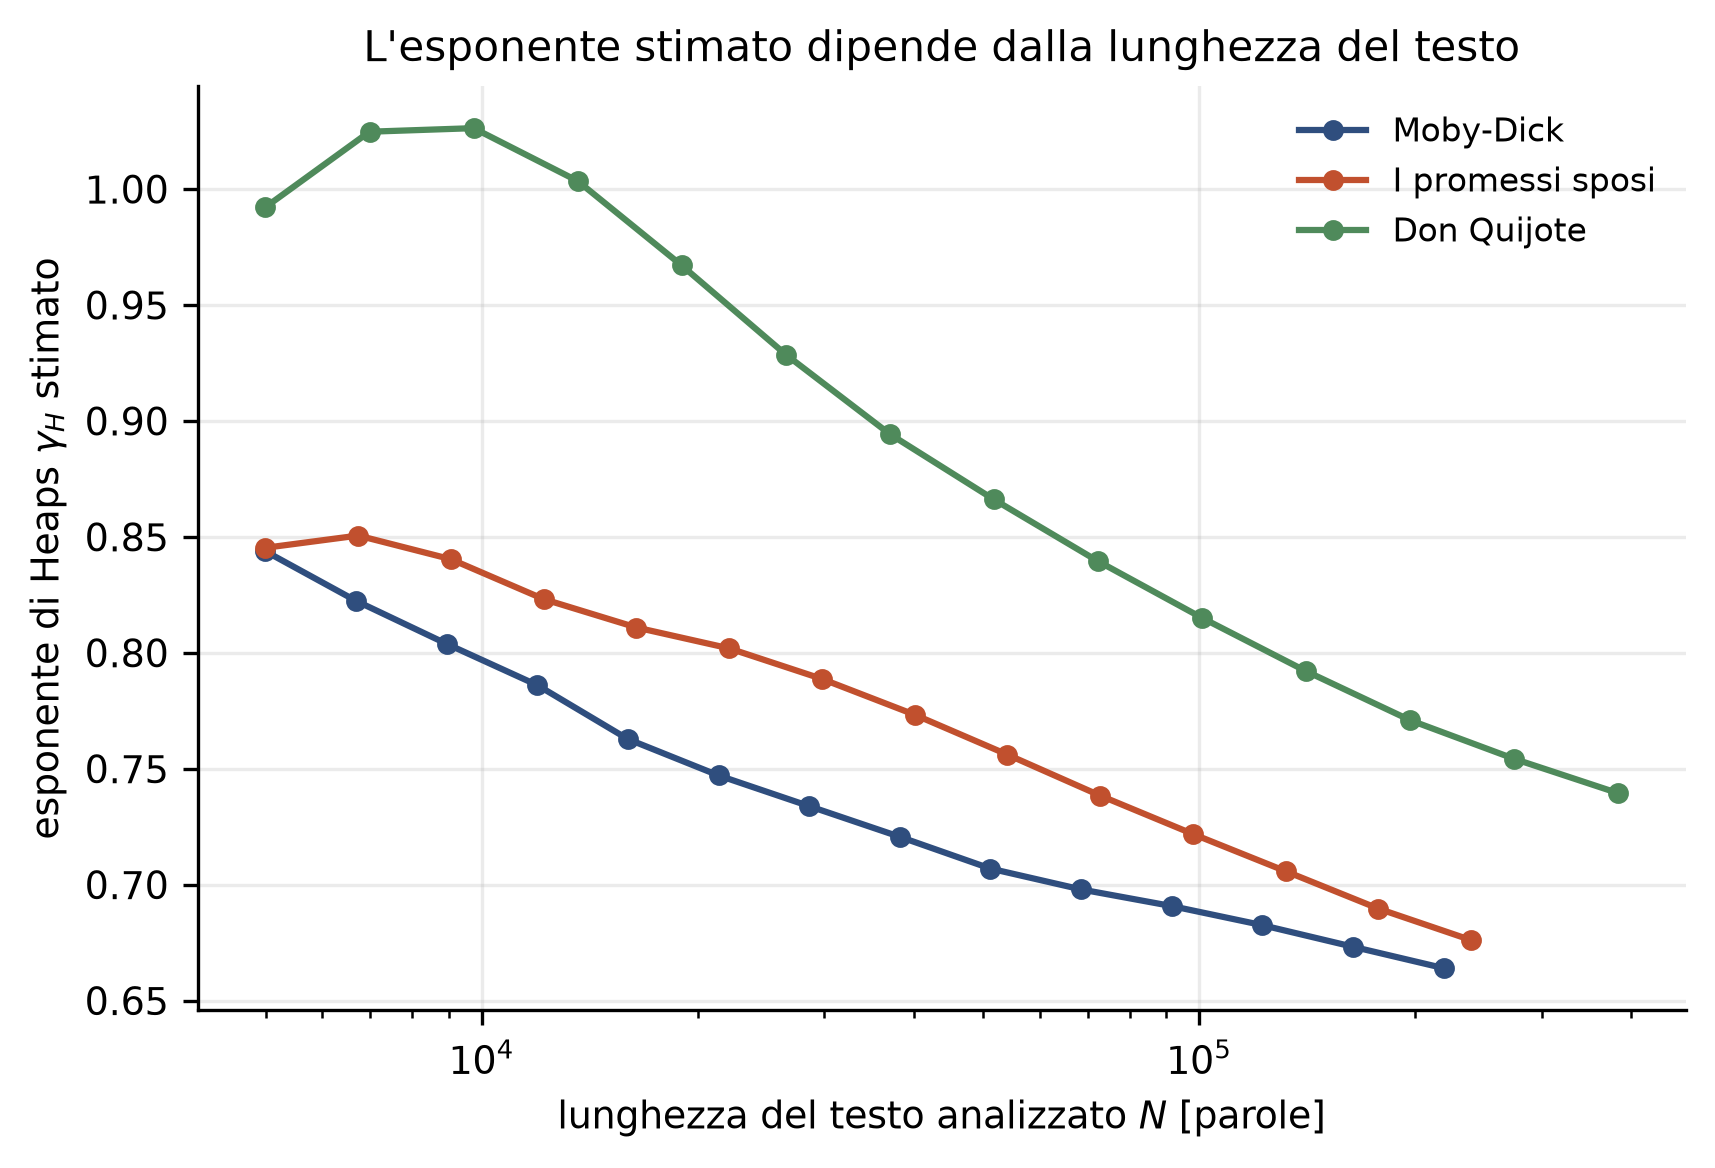
\includegraphics[width=0.78\textwidth]{figure/cap2_heaps_dimensione_finita.png}
  \caption{Esponente di Heaps stimato su prefissi di lunghezza crescente, per tre
  opere in tre lingue diverse, con regressione condotta nella regione $t > 1000$.
  La deriva è sistematica e comune a tutte e tre, ed è quindi una proprietà dello
  stimatore e non di una particolare opera: confrontare esponenti misurati su
  testi di lunghezza diversa non è lecito. Il §\ref{sec:scelte} riprende
  l'effetto su una sola opera, misurandone però l'entità su tutti gli stimatori
  impiegati in questa tesi.}
  \label{fig:heaps-finito}
\end{figure}

\paragraph{Il descrittore $R$.}
Sui testi generati automaticamente la difficoltà è più radicale. A bassa
temperatura di generazione il modello entra in un ciclo di ripetizione e cessa
di produrre parole nuove: la curva $|\mathcal{D}(t)|$ diventa piatta e
la~\eqref{eq:heaps} perde significato. Ad alta temperatura si verifica il caso
opposto, con quasi ogni parola nuova e curva prossima alla linearità. In
entrambe le situazioni la stima di $\gamma_H$ restituisce un numero privo di
contenuto, come mostrano le due curve estreme della Figura~\ref{fig:heaps}.

Per questa ragione in~\cite{mikhaylovskiy2025zipf} viene introdotto un
descrittore che resta definito in ogni regime. Detti $\mathcal{D}_1$ il
dizionario della prima metà del testo e $\mathcal{D}_2$ quello della seconda, si
pone
\begin{equation}
  R \;=\; \frac{|\mathcal{D}_2 \setminus \mathcal{D}_1|}{|\mathcal{D}_1|},
  \label{eq:R}
\end{equation}
cioè il rapporto fra il numero di parole che compaiono per la prima volta nella
seconda metà del testo e il numero di quelle che compaiono per la prima volta
nella prima. Un testo degenerato ha $R$ prossimo a zero, poiché la seconda metà
non introduce nulla di nuovo; un testo in cui ogni parola è nuova ha $R$
prossimo a uno. Sul corpus di opere letterarie intere usato
in~\cite{mikhaylovskiy2025zipf} il valore medio è $R = 0.17$ con deviazione
standard $0.05$.


% ---------------------------------------------------------------------
\section{Correlazioni a lungo raggio}
\label{sec:lrc}

Sia la legge di Zipf sia quella di Heaps ignorano l'ordine dei simboli. Per la
prima l'affermazione è immediata: la~\eqref{eq:zipf} dipende soltanto dai
conteggi delle parole, e un rimescolamento del testo li lascia invariati. Per la
seconda l'invarianza è meno diretta: rimescolando il testo la curva
$|\mathcal{D}(t)|$ cambia realizzazione, perché cambia l'ordine in cui le
parole compaiono per la prima volta, ma il suo andamento medio resta lo stesso, e con esso l'esponente
$\gamma_H$. Entrambe sono quindi proprietà del vocabolario, non della sequenza.

Per misurare le proprietà che dipendono dall'ordine occorre estrarre dal testo
un segnale, cioè una successione finita di valori reali, e studiarne le
correlazioni a scale diverse. La costruzione del segnale non è unica, e ogni
scelta mette in luce aspetti differenti: si può codificare la posizione delle
singole lettere o di classi di lettere, quella delle parole o di classi
grammaticali, oppure la lunghezza delle frasi. In tutti i casi si osserva che il
linguaggio esibisce correlazioni a lungo raggio, con una struttura che si
estende su molti ordini di grandezza~\cite{altmann2012,montemurro2002}.

% ---------------------------------------------------------------------
\subsection{Funzione di autocorrelazione}
\label{sec:acf}

Data una successione $x_1,\dots,x_N$, la funzione di autocorrelazione a distanza
$s$ è
\begin{equation}
  c(s) \;=\; \langle x_n x_{n+s}\rangle
  - \langle x_n\rangle\langle x_{n+s}\rangle ,
  \label{eq:acf}
\end{equation}
dove $\langle\cdot\rangle$ indica la media su tutte le posizioni $n$ compatibili
con la distanza $s$. La forma funzionale di $c(s)$ distingue i regimi di
correlazione.

Se i valori non sono correlati, $c(s)$ è identicamente nulla per $s \neq 0$. Se
$c(s)$ decade esponenzialmente,
$c(s) \sim e^{-s/s_0}$, il segnale si dice correlato a corto raggio: la costante
$s_0$ ha le dimensioni di una distanza e ne fissa la scala caratteristica, nel
senso che oltre poche volte $s_0$ la correlazione è numericamente
indistinguibile da zero. Esiste dunque una distanza tipica oltre la quale due
porzioni di segnale sono indipendenti, e il sistema non possiede struttura al di
là di essa.

Si dice invece che il segnale è correlato a lungo raggio quando il decadimento
segue la legge di potenza
\begin{equation}
  c(s) \;\sim\; s^{-\theta},
  \label{eq:acf-power}
\end{equation}
con $0<\theta<1$. In questo caso non esiste alcuna scala privilegiata: la
funzione~\eqref{eq:acf-power} è invariante di scala, cioè riscalare $s$ di un
fattore costante riscala $c$ di un fattore costante senza modificarne la forma,
e un certo grado di correlazione persiste a tutte le distanze.\footnote{L'esponente
qui indicato con $\theta$ è denotato con $\beta$ in~\cite{altmann2012} e con
$\gamma$ in altra parte della letteratura. Il simbolo è stato cambiato per
evitare la collisione con l'esponente di Heaps e con quello introdotto
nella~\eqref{eq:sigma}.}

La stima diretta di $\theta$ dalla~\eqref{eq:acf-power} è però problematica. Il
segnale è affetto da rumore e, soprattutto, da tendenze di origine esterna che
non sono oggetto di interesse: se la media $\langle x_n\rangle$ differisce fra
la prima e la seconda metà del segnale, come accade proprio quando le
correlazioni sono forti, la~\eqref{eq:acf} risulta distorta. L'esponente va
quindi stimato per via indiretta, e le due sottosezioni seguenti presentano i
due metodi impiegati in questa tesi.

% ---------------------------------------------------------------------
\subsection{Indicatore integrato}
\label{sec:integrato}

Il primo metodo è quello adottato da Altmann, Cristadoro e Degli
Esposti~\cite{altmann2012}, e si applica a segnali binari. Sia dato un testo
come successione simbolica $s = (s_1,\dots,s_N)$. Si definisce una condizione
locale $\mathcal{A}$ che genera la successione binaria
\begin{equation}
  x_k \;=\;
  \begin{cases}
    1 & \text{se $\mathcal{A}$ è soddisfatta in posizione $k$},\\
    0 & \text{altrimenti}.
  \end{cases}
  \label{eq:osservabile}
\end{equation}
L'osservabile può essere la presenza di una data lettera, di una data parola,
oppure l'appartenenza a una classe: per esempio se la lettera in posizione $k$ è
una vocale. L'unità di misura della distanza è il numero di simboli del livello
considerato, ed è questa scelta a rendere confrontabili fra loro una successione
di lettere e una di parole.

Posto
\begin{equation}
  X(t) \;=\; \sum_{j \le t} x_j ,
  \label{eq:conteggio}
\end{equation}
cioè il numero di occorrenze osservate nelle prime $t$ posizioni, si studia la
crescita della varianza del conteggio
\begin{equation}
  \sigma_X^2(t) \;=\; \langle X(t)^2\rangle - \langle X(t)\rangle^2
  \;\simeq\; t^{\gamma}, \qquad \gamma = 2 - \theta .
  \label{eq:sigma}
\end{equation}
La quantità $\sigma_X^2$ è, per costruzione, una somma delle correlazioni a
tutte le distanze inferiori a $t$, e come tale è numericamente assai più stabile
della~\eqref{eq:acf} stimata punto per punto.

Il discrimine fra correlazioni a corto e a lungo raggio non è l'ampiezza di
$c(s)$, ma la sua sommabilità. La~\eqref{eq:conteggio} è formalmente il
cammino percorso da un camminatore che a ogni passo avanza di $x_j$: se i passi
sono indipendenti, o abbastanza rapidamente decorrelati perché $\sum_s c(s)$
converga, vale il teorema del limite centrale e la varianza del cammino cresce
proporzionalmente al numero di passi. Si ha allora diffusione normale,
$\gamma = 1$, esattamente come per il moto browniano. Se invece la somma
diverge, cioè se $\theta \le 1$, i passi restano correlati a ogni scala, il
camminatore tende a proseguire nella direzione già intrapresa e si allontana
dall'origine più rapidamente: la diffusione è anomala e $1 < \gamma < 2$. Il
valore $\gamma = 1$ costituisce dunque il riferimento nullo di tutte le misure
di questo tipo.

La stima di $\gamma$ risente di effetti di tempo finito che la fanno
sottostimare~\cite{altmann2012}: tutti i valori riportati nei capitoli
sperimentali vanno letti come limiti inferiori.

% ---------------------------------------------------------------------
\subsection{Detrended fluctuation analysis}
\label{sec:dfa}

Il secondo metodo è la \emph{detrended fluctuation analysis}, introdotta da
Peng et al.~\cite{peng1994} e applicata ai testi generati automaticamente
in~\cite{lippi2019}. Rispetto all'indicatore integrato presenta il vantaggio
di rimuovere le tendenze locali, e risulta quindi applicabile anche a segnali
non stazionari, cioè segnali le cui proprietà statistiche, tipicamente la
media $\langle x_n \rangle$ o la varianza, non sono costanti lungo la
successione ma derivano lentamente da un estremo all'altro.

La distinzione fra tendenza e correlazione è essenziale, e non riguarda solo
l'origine delle due. Una tendenza è una deriva sistematica e regolare del valore
medio, sovrapposta al segnale da una causa esterna al sistema; una correlazione
è invece una proprietà statistica interna, che lega fra loro le fluttuazioni
attorno a quel valore medio. Il problema pratico è che entrambe producono lo
stesso effetto sulla~\eqref{eq:acf}, gonfiandola a grandi distanze, ed è quindi
necessario eliminare le prime per misurare le seconde. Si potrebbe pensare
sufficiente sottrarre una media mobile di ampiezza fissata, ma in questo modo si
introdurrebbe artificialmente nei dati proprio quella ampiezza come scala
caratteristica, distruggendo le altre.

Il segnale viene costruito codificando ogni carattere del testo con il proprio
rango di frequenza: al carattere più frequente si associa 1, al secondo 2, e
così via. Seguendo~\cite{lippi2019} la codifica avviene a livello di carattere e
conserva punteggiatura, cifre, maiuscole e lettere accentate. Ottenuta la
successione $x_i$ con $i = 1,\dots,N$, la procedura si articola in quattro
passi, qui presentati nella formulazione di~\cite{kantelhardt2001}.

\begin{enumerate}
  \item Si determina il profilo
    \begin{equation}
      Y(i) \;=\; \sum_{k=1}^{i}\bigl(x_k - \langle x\rangle\bigr),
      \label{eq:dfa-profilo}
    \end{equation}
    cioè lo scarto cumulato dalla media. La sottrazione della media non è
    strettamente necessaria, poiché verrebbe comunque eliminata dal detrending.
  \item Si divide il profilo in $N_s = \lfloor N/s \rfloor$ segmenti disgiunti
    di lunghezza $s$.
  \item In ciascun segmento si interpola ai minimi quadrati la tendenza locale,
    ottenendo il polinomio $Y_s(i)$ che approssima il profilo entro quel
    segmento. L'ordine del polinomio determina l'ordine delle tendenze rimosse:
    una DFA di ordine $n$ elimina le tendenze polinomiali fino al grado $n$. In
    questa tesi si impiega l'ordine 1, che rimuove le tendenze lineari locali;
    la robustezza dei risultati rispetto a questa scelta è verificata nel
    §\ref{sec:robustezza}.
  \item Si calcola lo scarto quadratico medio del profilo dalla propria
    tendenza locale, mediando su tutti i segmenti, e si ottiene la funzione di
    fluttuazione
    \begin{equation}
      F(s) \;=\; \left(\frac{1}{N}\sum_{i=1}^{N}
      \bigl(Y(i) - Y_s(i)\bigr)^2\right)^{1/2}.
      \label{eq:dfa-F}
    \end{equation}
\end{enumerate}

La fluttuazione cresce con la lunghezza dei segmenti $s$ e, per un segnale
correlato a lungo raggio, segue la legge di potenza
\begin{equation}
  F(s) \;\sim\; s^{\alpha_{\mathrm{DFA}}} .
  \label{eq:dfa-alpha}
\end{equation}
Per un segnale scorrelato, o correlato a corto raggio, si ha
$\alpha_{\mathrm{DFA}} = 1/2$. Valori superiori indicano correlazioni
persistenti: una fluttuazione positiva tende a essere seguita da un'altra
fluttuazione positiva, e il segnale conserva memoria della propria direzione.
Valori inferiori indicano correlazioni antipersistenti, in cui una fluttuazione
positiva tende a essere seguita da una negativa e il segnale tende a tornare
sui propri passi. Un cammino aleatorio dà $\alpha_{\mathrm{DFA}} = 3/2$: i suoi
incrementi sono scorrelati, ma la successione che ne risulta accumula ogni
deviazione senza riassorbirla, e le fluttuazioni crescono di conseguenza molto
più in fretta. Sul testo letterario di riferimento~\cite{lippi2019} riporta
$\alpha_{\mathrm{DFA}} \simeq 0.65$, contro $0.50$ misurato sulla sua versione
rimescolata: nettamente sopra il riferimento scorrelato e nettamente sotto
quello del cammino aleatorio.

% ---------------------------------------------------------------------
\subsection{Relazione fra i due metodi}
\label{sec:ponte}

I due metodi introdotti misurano la stessa proprietà, e i rispettivi esponenti
sono legati da una relazione semplice. Applicata alla medesima successione,
la~\eqref{eq:dfa-F} coincide, a meno del detrending, con la deviazione standard
del profilo alla scala $s$, cioè $F(s) \simeq \sigma_X(s)$. Elevando al quadrato
e usando la~\eqref{eq:sigma} si ottiene $F(s)^2 \simeq s^{\gamma}$, da cui
\begin{equation}
  \alpha_{\mathrm{DFA}} \;=\; \frac{\gamma}{2} \;=\; 1 - \frac{\theta}{2} .
  \label{eq:ponte}
\end{equation}
La stessa relazione, ricavata per altra via, è riportata
in~\cite{kantelhardt2001}. Nella~\eqref{eq:ponte} $\gamma$ è l'esponente di
crescita della varianza del conteggio definito nella~\eqref{eq:sigma}, mentre
$\theta$ è l'esponente di decadimento dell'autocorrelazione definito
nella~\eqref{eq:acf-power}; i tre esponenti sono dunque tre modi equivalenti di
esprimere la stessa proprietà del segnale.

La~\eqref{eq:ponte} costituisce il ponte fra le due parti sperimentali della
tesi: la diffusione normale $\gamma = 1$, riferimento nullo dell'analisi di
burstiness, corrisponde esattamente al valore $\alpha_{\mathrm{DFA}} = 1/2$,
riferimento nullo dell'analisi sui testi generati. Le due misure non coincidono
esattamente sui dati, poiché la detrended fluctuation analysis rimuove le
tendenze locali mentre l'indicatore integrato no; la differenza fra i due
risultati è informativa proprio quando il segnale non è stazionario.

Un caso limite si presenta con frequenza nei testi generati a bassa
temperatura. Se il testo degenera in un ciclo di ripetizione,
la successione $x_i$ diventa quasi periodica e il profilo~\eqref{eq:dfa-profilo}
oscilla invece di allontanarsi dall'origine: la fluttuazione satura oltre la
lunghezza del periodo e $\alpha_{\mathrm{DFA}}$ scende verso zero. Un esponente
molto basso non segnala quindi assenza di struttura, ma struttura periodica, e
va interpretato congiuntamente a un indicatore diretto di ripetizione.


% ---------------------------------------------------------------------
\section{Burstiness e statistica degli intervalli}
\label{sec:burst}

Le sezioni precedenti permettono di stabilire se un testo possieda correlazioni
a lungo raggio. Questa sezione introduce gli strumenti necessari a stabilire
l'origine di tali correlazioni, che è la domanda posta in~\cite{altmann2012} e
ripresa nella seconda parte sperimentale.

Il punto di partenza è un'osservazione elementare sulla distribuzione delle
parole lungo il testo. Non tutte le parole si distribuiscono allo stesso modo:
alcune ricorrono in modo pressoché uniforme dall'inizio alla fine, altre si
addensano nelle sezioni che trattano l'argomento cui appartengono e sono quasi
assenti altrove. La Figura~\ref{fig:barcode} rende visibile la differenza. Ogni
barra verticale segna una posizione in cui la parola compare; nel primo pannello
la parola è un articolo, nel secondo il nome di un personaggio.

\begin{figure}[htbp]
  \centering
  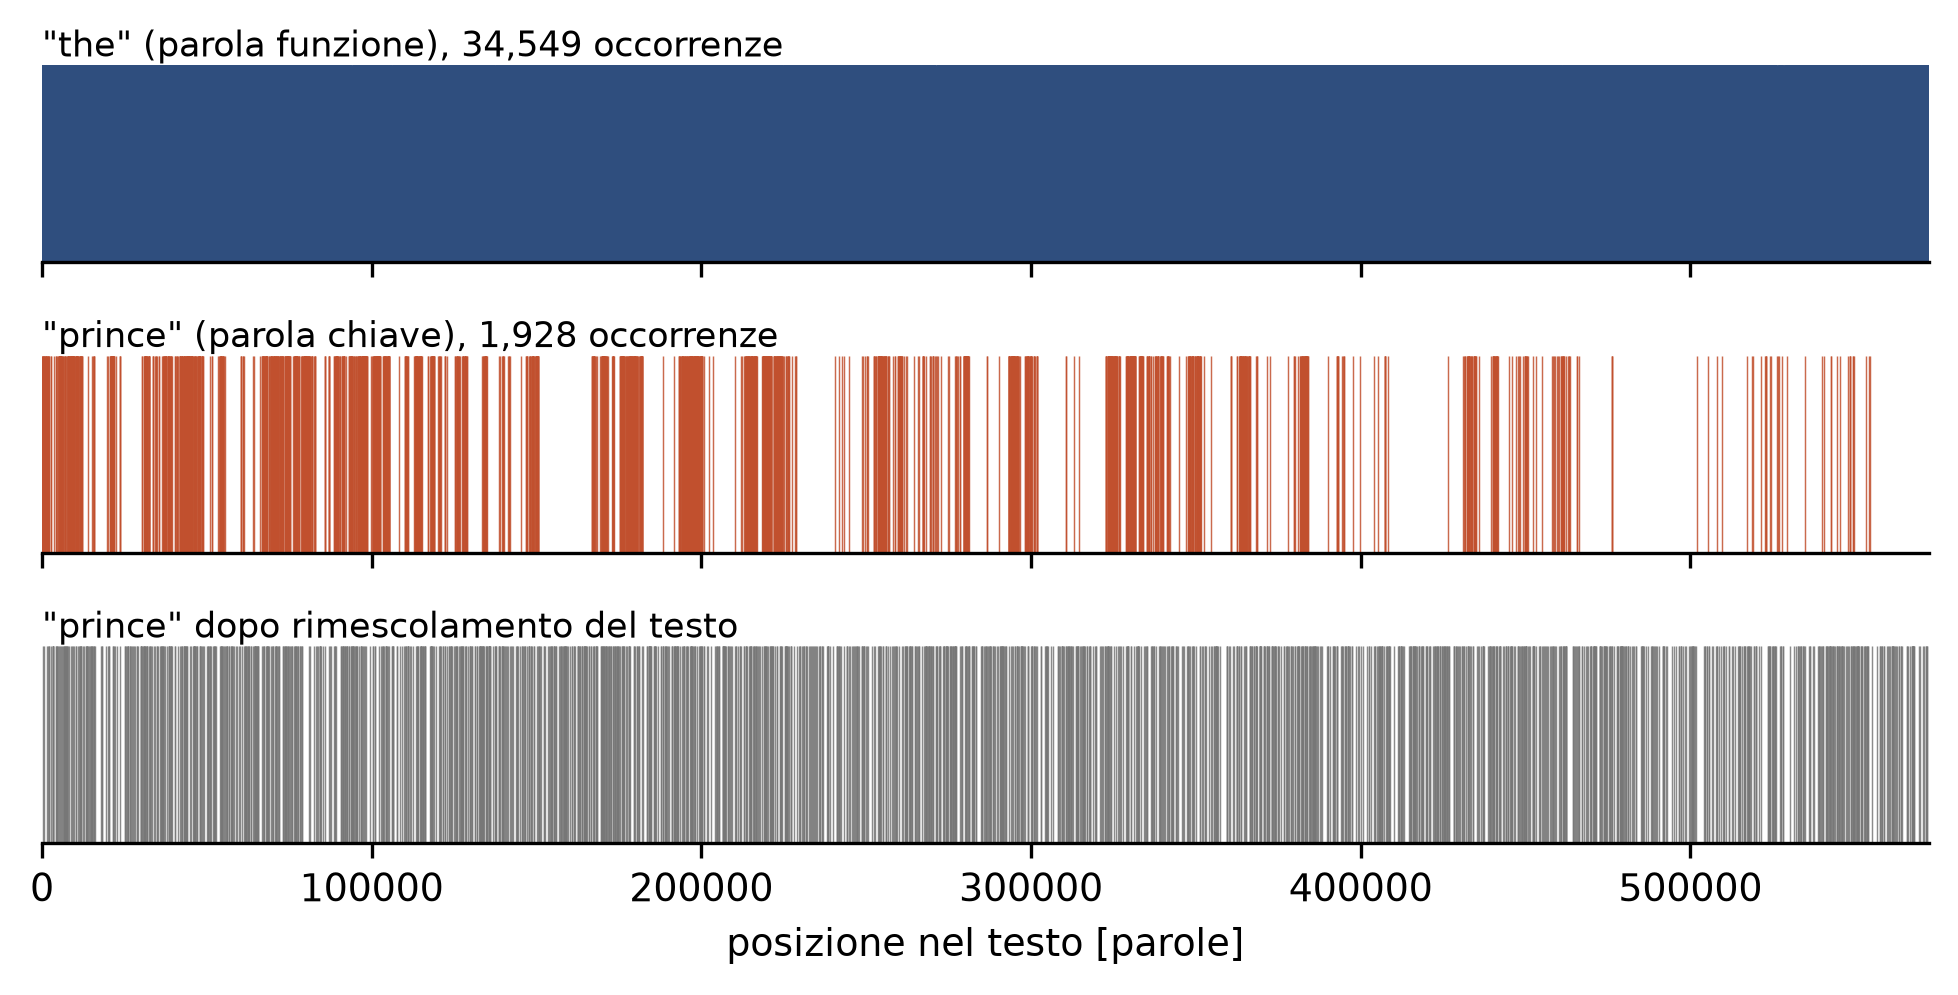
\includegraphics[width=\textwidth]{figure/cap2_burstiness_barcode.png}
  \caption{Posizioni di occorrenza di due parole in \emph{Guerra e pace}. La
  parola funzione \emph{the} riempie il testo in modo uniforme e il pannello
  appare come una banda piena. La parola chiave \emph{prince} si addensa invece
  in gruppi separati da lunghi vuoti, che corrispondono alle porzioni di romanzo
  in cui il personaggio non compare. Il terzo pannello riporta le occorrenze di
  \emph{prince} dopo aver rimescolato le parole del testo: i conteggi sono
  identici, ma i gruppi scompaiono. La struttura visibile nel secondo pannello
  è dunque una proprietà dell'ordine, non delle frequenze.}
  \label{fig:barcode}
\end{figure}

Il fenomeno illustrato dal secondo pannello prende il nome di
\emph{burstiness}: le occorrenze non sono sparse indipendentemente, ma
raggruppate in raffiche separate da intervalli lunghi. Il terzo pannello mostra
perché si tratti di una proprietà dell'ordine e non del vocabolario: il
rimescolamento conserva esattamente il numero di occorrenze, e con esso la legge
di Zipf, ma distrugge la struttura.

Per quantificare il fenomeno si torna alla successione binaria definita
nella~\eqref{eq:osservabile} e si considerano gli intervalli
$\tau_1, \tau_2, \dots$ fra occorrenze consecutive, cioè le distanze in numero
di simboli fra un $1$ e il successivo. La loro distribuzione di probabilità
viene indicata con $p(\tau)$ ed è l'oggetto centrale di questa sezione: tutta
l'informazione sull'ordine che il conteggio delle occorrenze non cattura è
contenuta in $p(\tau)$ e nelle correlazioni fra intervalli successivi.

Il termine di paragone naturale è il processo di Poisson, cioè il processo in
cui ogni posizione ha la stessa probabilità di ospitare un'occorrenza,
indipendentemente da tutte le altre. È il modello del «nessuna struttura»: se le
occorrenze di \emph{prince} fossero poissoniane, il secondo pannello della
Figura~\ref{fig:barcode} sarebbe indistinguibile dal terzo. Per un processo di
Poisson gli intervalli sono distribuiti esponenzialmente e indipendenti fra
loro, e si dimostra che la loro deviazione standard eguaglia la media,
$\sigma_\tau = \langle\tau\rangle$.

Si misura quindi la burstiness con il coefficiente di variazione
\begin{equation}
  \mathrm{cv} \;=\; \frac{\sigma_\tau}{\langle\tau\rangle},
  \label{eq:cv}
\end{equation}
pari a 1 nel caso poissoniano, maggiore di 1 quando le occorrenze si addensano
in raffiche separate da vuoti lunghi e minore di 1 quando sono distribuite in
modo più regolare di quanto il caso comporti. Una misura equivalente, ma
limitata all'intervallo $[-1,1]$ e quindi più comoda per il confronto fra
sequenze diverse, è l'indice proposto da Goh e Barabási~\cite{goh2008},
\begin{equation}
  B \;=\; \frac{\sigma_\tau - \langle\tau\rangle}
                {\sigma_\tau + \langle\tau\rangle} .
  \label{eq:goh}
\end{equation}

% ---------------------------------------------------------------------
\subsection{Le due origini delle correlazioni}
\label{sec:origini}

Il contributo centrale di~\cite{altmann2012} consiste nell'osservare che una
varianza del conteggio che cresce più che linearmente può avere due origini
distinte. Il legame è fornito dallo spettro di potenza a frequenza nulla.

Lo spettro di potenza $S(\omega)$ di una successione descrive come la sua
varianza si distribuisce fra le diverse frequenze $\omega$, ed è la trasformata
di Fourier della funzione di autocorrelazione. Il valore a frequenza nulla,
$S(0)$, raccoglie il contributo delle fluttuazioni più lente, quelle su scale
comparabili con la lunghezza dell'intera successione: è quindi la quantità che
diverge esattamente quando esistono correlazioni a lungo raggio, e che resta
finita quando le correlazioni sono sommabili. Per una successione di occorrenze
descritta dagli intervalli $\tau_i$ vale
\begin{equation}
  S(0) \;=\; \frac{\sigma_\tau^2}{\langle\tau\rangle^3}
  \left(1 + 2\sum_{k\ge1} c_\tau(k)\right),
  \label{eq:eq4}
\end{equation}
dove $c_\tau(k)$ è l'autocorrelazione della successione degli intervalli, cioè
la correlazione fra $\tau_i$ e $\tau_{i+k}$.

La~\eqref{eq:eq4} è il perno dell'intera analisi, perché mostra che $S(0)$ può
divergere in due modi indipendenti. Il primo è la divergenza di $\sigma_\tau$,
cioè una coda pesante di $p(\tau)$: il testo contiene vuoti così lunghi che la
varianza degli intervalli non converge. Il secondo è la non sommabilità di
$c_\tau(k)$, cioè il fatto che gli intervalli siano essi stessi correlati fra
loro. Nella formula resta implicito che cosa questo comporti: $c_\tau(k) > 0$
significa che a un intervallo più lungo della media tende a seguirne un altro
più lungo della media, e quindi che i vuoti si
raggruppano fra loro invece di alternarsi ai riempimenti. Anche con una
$p(\tau)$ a varianza finita, un simile raggruppamento produce fluttuazioni
lente del conteggio e fa divergere la somma.

I due meccanismi sono distinti, perché l'uno riguarda quanto sono lunghi i
vuoti e l'altro come sono disposti, e la~\eqref{eq:eq4} da sola non li separa.

Nei testi reali, di lunghezza finita e con la coda tagliata
(§\ref{sec:coda}), nessuna delle due quantità diverge davvero: ciò che si
misura sono i loro analoghi a finestra finita, e i due null model del
§\ref{sec:null} servono appunto a separarli senza dover decidere quale delle
due divergenze sarebbe realizzata nel limite.

% ---------------------------------------------------------------------
\subsection{I null model A1 e A2}
\label{sec:null}

La separazione si ottiene con due rimescolamenti controllati, costruiti in modo
da distruggere selettivamente uno solo dei due meccanismi.

Il primo, indicato con A1, permuta gli zeri e gli uni della successione binaria.
Conserva soltanto il numero di occorrenze e distrugge tanto la coda di $p(\tau)$
quanto $c_\tau(k)$: è il rimescolamento già illustrato nel terzo pannello della
Figura~\ref{fig:barcode}. Ha funzione di controllo, poiché il risultato è noto a
priori: deve restituire un esponente $\hat\gamma_{A1}$ prossimo a 1, e un valore
diverso segnala un difetto della procedura di misura prima ancora che una
proprietà dei dati.

Il secondo, indicato con A2, permuta fra loro gli intervalli $\tau_i$ senza
alterarne l'insieme. Conserva quindi esattamente $p(\tau)$, e con essa
$\sigma_\tau$, ma distrugge ogni correlazione fra intervalli successivi.
L'esponente risultante $\hat\gamma_{A2}$ isola dunque il solo contributo della
burstiness.

Poiché A2 rimuove un contributo che è di norma non negativo, ci si attende la
disuguaglianza
\begin{equation}
  \hat\gamma \;\ge\; \hat\gamma_{A2},
  \label{eq:disug1}
\end{equation}
che in~\cite{altmann2012} è riportata come regolarità empirica, non come
conseguenza necessaria, e che il §\ref{sec:coda-risultati} verifica
direttamente su tutti i corpora. Fornisce quindi un ulteriore controllo interno
alla misura. Risulta naturale
definire la quota di burstiness
\begin{equation}
  q \;=\; \frac{\hat\gamma_{A2} - 1}{\hat\gamma - 1},
  \label{eq:quota}
\end{equation}
prossima a 1 quando la correlazione proviene interamente dalla coda di $p(\tau)$
e prossima a 0 quando proviene interamente da $c_\tau(k)$: $q$ misura cioè quale
frazione dell'eccesso di correlazione sia attribuibile alla sola burstiness.

Il denominatore della~\eqref{eq:quota} è però piccolo nei corpora poco
correlati, dove $\hat\gamma$ è di poco superiore a 1, e $q$ risulta di
conseguenza uno stimatore rumoroso. Per questa ragione, in questo lavoro $q$
viene calcolata separatamente per ciascun documento e riassunta con mediana e
quartili anziché come rapporto fra medie: si tratta di una scelta metodologica
adottata qui, non di una prescrizione della letteratura, motivata dal fatto che
il rapporto fra due medie non coincide con la media dei rapporti quando il
denominatore ha varianza comparabile al proprio valore.

% ---------------------------------------------------------------------
\subsection{Coda della distribuzione degli intervalli}
\label{sec:coda}

Il legame quantitativo fra burstiness ed esponente di correlazione richiede una
forma esplicita per $p(\tau)$. Assumendo una legge di potenza pura e intervalli
scorrelati si ottiene
\begin{equation}
  p(\tau) \sim \tau^{-\mu}, \quad c_\tau(k) = \delta(k), \quad 2 < \mu < 3
  \;\Longrightarrow\;
  \gamma = 4 - \mu .
  \label{eq:eq8}
\end{equation}
La condizione $2<\mu<3$ individua il regime in cui la media di $\tau$ esiste ma
la varianza diverge, ed è esattamente il regime in cui la~\eqref{eq:cv} non
converge al crescere della lunghezza del testo.

La legge di potenza pura è però un modello idealizzato, e lo stesso
\cite{altmann2012} lo riconosce nel formulare la~\eqref{eq:eq8}. Scendendo
nella gerarchia linguistica i vuoti lunghi vengono spezzati: una lettera che
compone una parola chiave compare anche in tutte le altre parole del testo, e i
lunghi intervalli in cui la parola chiave è assente si riempiono di occorrenze
dovute ad altre parole. Esiste quindi una lunghezza $\tau_c$ oltre la quale gli
intervalli, semplicemente, non si osservano più: è il cut-off che quel lavoro
introduce con questo stesso argomento, senza però stimarlo. Il modello
realistico è la legge di potenza troncata
\begin{equation}
  p(\tau) \;\sim\; \tau^{-\mu}\,e^{-\tau/\tau_c},
  \label{eq:troncata}
\end{equation}
che ha due vantaggi rispetto alla forma pura. Il primo è descrittivo: separa due
proprietà distinte della coda, la pendenza $\mu$ nella regione intermedia e la
distanza $\tau_c$ alla quale la coda viene tagliata, mentre un fit con la sola
legge di potenza le confonde in un unico esponente apparente. Il secondo è che
rende la distribuzione normalizzabile e a varianza finita per ogni $\mu$,
eliminando la necessità di assumere $2<\mu<3$. In presenza di cut-off la
burstiness contribuisce solo per distanze inferiori a $\tau_c$, e
la~\eqref{eq:eq8} non vale più come uguaglianza ma come disuguaglianza,
\[
  \hat\gamma_{A2} \;\le\; 4 - \mu ,
\]
che vincola dall'alto l'esponente misurato sul null model A2.

Nella~\eqref{eq:troncata} $\mu$ e $\tau_c$ agiscono sulla forma della coda in
modo parzialmente sovrapposto: rendere la coda più ripida aumentando $\mu$
produce quasi lo stesso effetto che tagliarla prima riducendo $\tau_c$. Di
conseguenza esistono molte coppie $(\mu, \tau_c)$ diverse fra loro che
descrivono i dati quasi altrettanto bene, cioè che rendono quasi identica la
verosimiglianza, la probabilità di osservare i dati raccolti sotto quei valori
dei parametri. La conseguenza pratica è duplice: gli intervalli di confidenza
vanno calcolati per profilo, esplorando cioè la verosimiglianza al variare di
un parametro con l'altro riottimizzato, e non con la formula asintotica che
presuppone parametri indipendenti; e $\mu$ non va riportato separatamente dal
$\tau_c$ che lo accompagna, perché da solo non identifica la coda.

% ---------------------------------------------------------------------
\subsection{Effetti di dimensione finita}
\label{sec:lunghezza}

Per la legge di potenza pura, quando $\mu<3$ la varianza di $p(\tau)$ diverge e
la stima di $\sigma_\tau$ non converge. Con il taglio della~\eqref{eq:troncata}
i momenti sono invece finiti, ma $\tau_c$ è esso stesso una grandezza che
dipende dalla finestra, e la conseguenza osservabile è la medesima:
la~\eqref{eq:cv} cresce monotonamente con la finestra di osservazione,
poiché finestre più lunghe campionano vuoti più lunghi. Lo stesso vale, in
misura diversa, per l'esponente di Heaps e per il MAPE, come già mostrato nella
Figura~\ref{fig:heaps-finito} del §\ref{sec:heaps}.

La deriva non è un difetto di stima che una procedura migliore potrebbe
eliminare: è una proprietà delle quantità stesse, che su una finestra finita non
hanno un valore limite. Ne discendono vincoli su come i confronti possono essere
condotti, ed è il Capitolo~\ref{cap:metodi} a fissarli, insieme alla misura
dell'entità dell'effetto sui corpora effettivamente impiegati.


% ---------------------------------------------------------------------
\subsection{Entropia degli intervalli}
\label{sec:entropia-intervalli-def}

Il coefficiente di variazione della~\eqref{eq:cv} ha due limiti che il
§\ref{sec:lunghezza} rende evidenti. Il primo è la dipendenza dalla lunghezza
di analisi, che ne impedisce il confronto fra corpora misurati su finestre
diverse. Il secondo è più sottile: $\mathrm{cv}$ è un rapporto e quindi non
cambia se tutti gli intervalli vengono moltiplicati per una costante, ma nei
confronti fra corpora la dilatazione non è uniforme. Quando il tempo si conta in
caratteri, un corpus con frasi mediamente più lunghe produce intervalli più
lunghi ai soli livelli definiti su unità linguistiche, e non a quello dei
caratteri: la scala dei $\tau$ non è la stessa nei due corpora e ogni
differenza ne risente.

Serve quindi una misura di irregolarità che dipenda dalla forma della
distribuzione degli intervalli e non dalla loro scala. Si adotta a questo
scopo l'entropia differenziale del logaritmo degli intervalli, stimata per
spaziature d'ordine con lo stimatore di Vasicek~\cite{vasicek1976}, diminuita
di quella che si otterrebbe da un processo di Poisson con lo stesso numero di
eventi e la stessa media: \begin{equation} J \;=\; h(\ln\tau) \;-\;
h_{\mathrm{Poisson}}(n, \langle\tau\rangle). \label{eq:entropia-intervalli}
\end{equation}

Le due operazioni rispondono ai due limiti. Prendere il logaritmo rende $J$
invariante per dilatazione: moltiplicare tutti i $\tau$ per una costante trasla
$\ln\tau$ senza modificarne l'entropia differenziale, cosicché la diversa
lunghezza delle frasi non produce alcun effetto. Sottrarre il valore poissoniano
fissa lo zero sul processo privo di struttura, come per la~\eqref{eq:cv}, ma con
un vantaggio ulteriore: il termine sottratto viene simulato con lo stesso
stimatore e con gli stessi $n$ e $\langle\tau\rangle$ del dato osservato, per
cui il bias dello stimatore si cancella in larga parte nella differenza invece
di sommarsi.

\paragraph{Fin dove l'invarianza tiene.}
L'argomento appena dato riguarda una distribuzione continua. Gli intervalli fra
occorrenze in un testo sono invece numeri interi, e l'arrotondamento agli interi
non commuta con la dilatazione: comprimere una distribuzione fino a intervalli
di poche unità ne cancella la forma, e $J$ ne risente. Il pannello A della
Figura~\ref{fig:invarianza-J} misura l'entità del fenomeno moltiplicando per una
costante gli intervalli generati da una stessa legge. Per
$\langle\tau\rangle \gtrsim 30$ le curve sono piatte entro due centesimi di bit
e l'invarianza tiene; per $\langle\tau\rangle = 5$ una dilatazione di un fattore
cinquanta sposta $J$ di $0.59$ bit. L'invarianza è dunque asintotica nel valore
medio degli intervalli, non esatta.

La distinzione ha una conseguenza pratica sui livelli linguistici. Ai due
livelli lessicali, dove la diversa lunghezza delle frasi si fa sentire,
l'intervallo medio nei corpora del Capitolo~\ref{cap:risultati2} vale fra $340$
e $1900$ caratteri, quindi in pieno regime asintotico. Ai livelli delle lettere e
degli spazi, dove l'intervallo medio scende sotto la decina, i valori di $J$
risentono della quantizzazione e vanno letti come descrittori relativi, validi
per confrontare corpora misurati allo stesso modo e non come distanze assolute
dal processo di Poisson.

Il pannello B della stessa figura verifica la cancellazione del bias facendo
crescere il numero di intervalli da $30$ a $1000$ su cinque leggi di forma nota.
La deriva residua non supera $0.07$ bit su un intervallo in cui $n$ cambia di un
fattore trentatré, ed è massima sulle distribuzioni log-normali. La
cancellazione è quindi buona ma non completa, e differenze di $J$ inferiori a un
decimo di bit fra sequenze di numerosità molto diversa non sono interpretabili.

\begin{figure}[htbp]
  \centering
  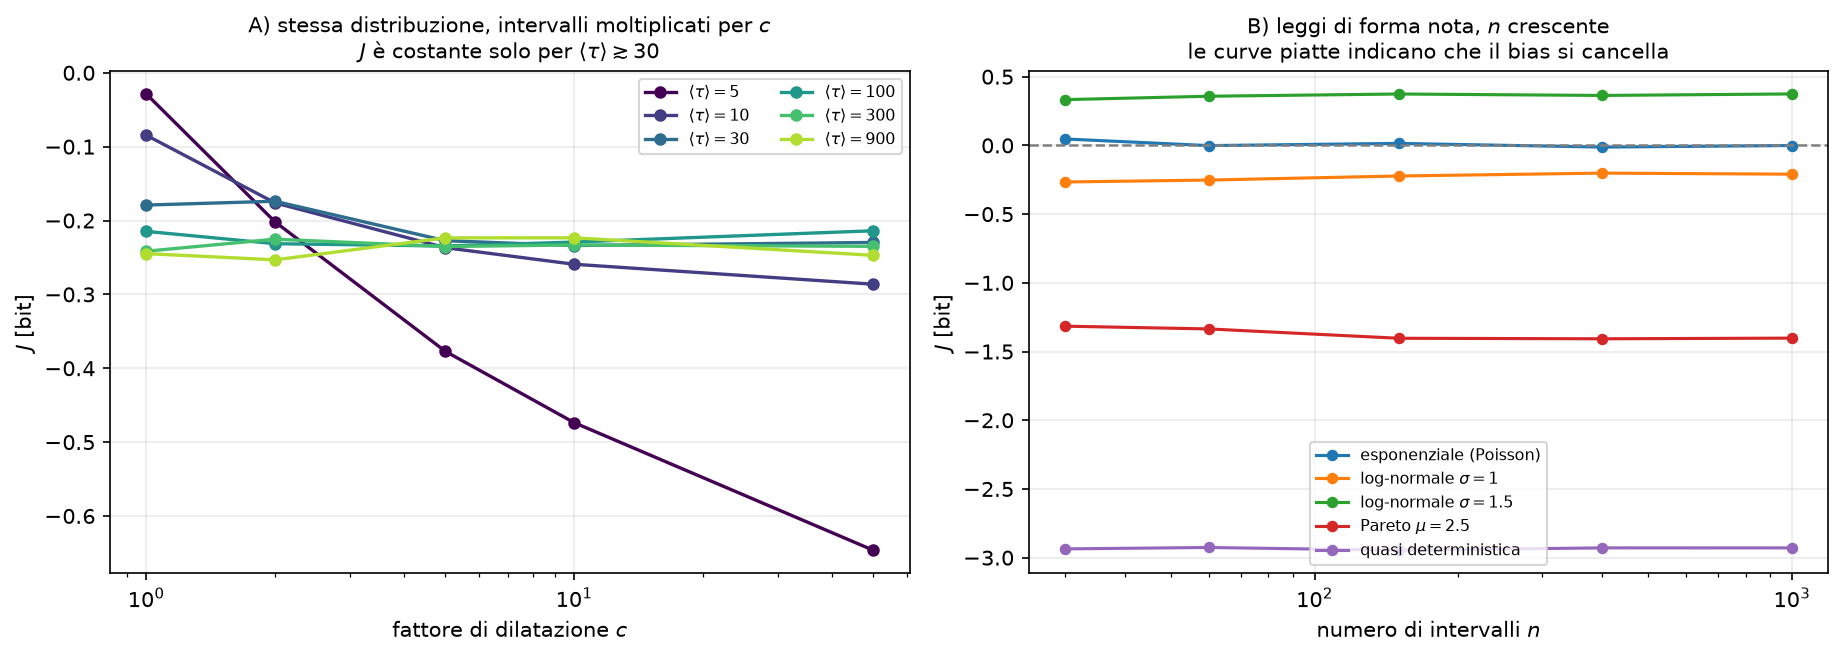
\includegraphics[width=\textwidth]{figure/cap2_invarianza_J.png}
  \caption{Limiti di validità della~\eqref{eq:entropia-intervalli}, misurati
  sullo stimatore effettivamente impiegato. A: intervalli estratti da una stessa
  legge log-normale e moltiplicati per un fattore $c$, per sei valori
  dell'intervallo medio di partenza; una curva piatta indica invarianza. Sotto
  $\langle\tau\rangle \simeq 30$ la quantizzazione agli interi la distrugge. B:
  $J$ su cinque leggi di forma nota al crescere del numero di intervalli; lo
  scostamento fra gli estremi quantifica il bias che la sottrazione del termine
  poissoniano non elimina.}
  \label{fig:invarianza-J}
\end{figure}

Valori positivi di $J$ indicano intervalli distribuiti in modo più irregolare di
un processo di Poisson, valori negativi una regolarità superiore a quella del
caso. La quantità non compare in nessuno dei lavori di riferimento ed è
introdotta qui; il §\ref{sec:entropia-intervalli} ne verifica la stabilità
rispetto alla lunghezza di analisi e la impiega per neutralizzare l'effetto
appena descritto.


% ---------------------------------------------------------------------
\section{Entropia e compressione}
\label{sec:entropia}

Il concetto di disordine di un testo e la nozione di entropia sono già stati
introdotti nel Capitolo~\ref{cap:introduzione}. Trattandosi di un concetto
centrale per questo lavoro, in questa sezione viene definito in modo formale e
ne viene esplicitato il legame con gli algoritmi di compressione, che è lo
strumento con cui l'entropia verrà effettivamente stimata sui testi.

% ---------------------------------------------------------------------
\subsection{Entropia e predicibilità}
\label{sec:entropia-def}

Si consideri una sorgente che emette simboli da un alfabeto finito
$\mathcal{X}$. Per una singola variabile aleatoria $X$ che assume il valore
$x \in \mathcal{X}$ con probabilità $p(x)$, l'entropia di
Shannon~\cite{shannon1948} è
\begin{equation}
  H(X) \;=\; -\sum_{x \in \mathcal{X}} p(x) \log_2 p(x),
  \label{eq:H-singola}
\end{equation}
espressa in bit, e misura l'incertezza media sull'esito dell'estrazione.

I simboli di un testo non sono però indipendenti, e l'entropia di una singola
lettera non descrive la sorgente: sapere che in inglese la lettera più frequente
è \emph{e} dice poco, mentre sapere che dopo \emph{th} segue quasi sempre
\emph{e} dice molto. Occorre quindi considerare blocchi di simboli. Detta
$H(X_1,\dots,X_n)$ l'entropia congiunta di un blocco di lunghezza $n$, definita
dalla~\eqref{eq:H-singola} applicata alla distribuzione congiunta dei blocchi, si
definisce il tasso di entropia della sorgente come
\begin{equation}
  h \;=\; \lim_{n\to\infty} \frac{H(X_1,\dots,X_n)}{n} .
  \label{eq:tasso-entropia}
\end{equation}
Il limite esiste per sorgenti stazionarie ed ergodiche~\cite{cover2006} e
quantifica l'incertezza media per simbolo una volta tenuto conto di tutte le
dipendenze, comprese quelle a lunga distanza. È questa, e non
la~\eqref{eq:H-singola}, la quantità pertinente per un testo.

Il teorema della codifica di sorgente~\cite{cover2006} lega $h$ alla
comprimibilità: il tasso di entropia è un limite inferiore alla lunghezza media
per simbolo di qualunque codifica senza perdita. Stimare l'entropia di un testo
e stimarne la comprimibilità sono quindi, entro le approssimazioni del caso, lo
stesso problema.

Il legame si comprende in modo intuitivo tornando ai casi limite della
Tabella~\ref{tab:tre-regimi}. Un algoritmo di compressione senza perdita opera
sostituendo alle porzioni di testo che si ripetono un riferimento
all'occorrenza precedente, più breve del testo che rimpiazza. Nel testo monotono
il medesimo gruppo di parole ricorre per l'intera lunghezza del documento: dopo
la prima occorrenza tutto il resto è un riferimento, il file compresso è
minuscolo e il tasso di entropia è prossimo a zero, perché il simbolo successivo
è quasi sempre determinato da quelli che lo precedono. Nella sequenza casuale,
al contrario, nessuna porzione si ripete: non esiste nulla cui fare riferimento,
il compressore non guadagna nulla e il tasso di entropia è massimo, perché ogni
simbolo è imprevedibile a partire dai precedenti. Il linguaggio naturale si
colloca fra i due estremi, e la quantità di compressione che ammette è una
misura diretta di quanta struttura possiede.

\paragraph{Stimatori di Lempel--Ziv.}
La stima diretta di $h$ dalla~\eqref{eq:tasso-entropia} per conteggio di blocchi
è impraticabile: il numero di blocchi distinti di lunghezza $n$ cresce
esponenzialmente con $n$, e la dimensione campionaria necessaria a stimarne le
probabilità cresce di conseguenza. Nessun testo reale è abbastanza lungo.

Si ricorre allora agli stimatori della famiglia Lempel--Ziv~\cite{ziv1977},
che aggirano il problema misurando le ripetizioni invece delle probabilità.
L'idea è la seguente: si scorre la successione e, a ogni posizione $i$, si cerca
la più lunga sottostringa che inizi in $i$ e sia già comparsa in precedenza,
detta $\Lambda_i$ la sua lunghezza. In un testo molto ripetitivo i match sono
lunghi, in un testo casuale sono corti. Si dimostra che, per una sorgente
stazionaria ed ergodica, la lunghezza media di tali match cresce come il
logaritmo della finestra esplorata e che
\begin{equation}
  h \;=\; \lim_{n\to\infty}
  \left\langle \frac{\log_2 n}{\Lambda_i} \right\rangle ,
  \label{eq:lz-entropia}
\end{equation}
dove la media è presa sulle posizioni $i$. La~\eqref{eq:lz-entropia} converge
assai più rapidamente del conteggio di blocchi e mantiene buone proprietà anche
in presenza di correlazioni a lungo raggio, che è la ragione per cui viene
adottata qui: le sorgenti considerate in questa tesi hanno, per costruzione,
memoria lunga.

% ---------------------------------------------------------------------
\subsection{Stima della cross-entropia e della divergenza}
\label{sec:crossparsing}

Le quantità introdotte finora descrivono un testo singolo. Per confrontare due
testi occorre la cross-entropia, che misura il costo di codificare un testo
usando la statistica di un altro.

L'algoritmo di cross-parsing di Ziv e Merhav~\cite{ziv1993} estende
la~\eqref{eq:lz-entropia} a due successioni. Data la successione $x$ da
misurare e la successione di riferimento $y$, si scorre $x$ da sinistra a destra
e la si decompone in frasi successive, dove ogni frase è la più lunga
sottostringa che, a partire dalla posizione corrente, compaia da qualche parte
in $y$; raggiunto il punto in cui il match si interrompe, si chiude la frase e
se ne apre una nuova. Il numero di frasi così ottenute viene indicato con
$c(x|y)$ ed è la quantità che misura la somiglianza fra i due testi: se $x$ e
$y$ provengono dalla stessa sorgente, le frasi sono lunghe e poche; se
provengono da sorgenti diverse, i match si interrompono presto e le frasi sono
molte. La stima della cross-entropia è
\begin{equation}
  h(x \,|\, y) \;=\; \frac{c(x|y)\,\log_2 |y|}{|x|},
  \label{eq:crossparsing}
\end{equation}
espressa in bit per simbolo, dove $|x|$ e $|y|$ sono le lunghezze delle due
successioni.

La divergenza di Kullback--Leibler è lo strumento con cui si quantifica quanto
due distribuzioni di probabilità differiscano fra loro. Date due distribuzioni
$P$ e $Q$ sullo stesso alfabeto, essa è definita come
\begin{equation}
  D(P\|Q) \;=\; \sum_{x} P(x) \log_2 \frac{P(x)}{Q(x)}
  \;=\; H_P(Q) - H(P),
  \label{eq:kl-def}
\end{equation}
dove $H_P(Q)$ è la cross-entropia fra le due distribuzioni. La~\eqref{eq:kl-def}
si interpreta come il numero medio di bit sprecati per simbolo codificando una
sorgente $P$ con un codice ottimizzato per $Q$: vale zero se e solo se
$P = Q$ ed è positiva altrimenti.

In termini di successioni, la~\eqref{eq:kl-def} si stima come differenza fra due
cross-entropie: dividendo $x$ in due metà $x_1$ e $x_2$ e prendendo da $y$ un
prefisso $y_1$ della stessa lunghezza di $x_1$, si pone
\begin{equation}
  D(x \,\|\, y) \;=\; h(x_2 \,|\, y_1) \;-\; h(x_2 \,|\, x_1) .
  \label{eq:kl}
\end{equation}
La seconda metà di $x$ viene cioè codificata due volte, una volta usando come
riferimento un testo estraneo e una volta usando la prima metà di $x$ stesso, e
si misura quanto costa in più la prima operazione.

L'appaiamento delle lunghezze dei due riferimenti non è un dettaglio.
La~\eqref{eq:crossparsing} dipende dalla lunghezza del riferimento, poiché un
riferimento più lungo contiene più sottostringhe e produce una cross-entropia
minore a parità di sorgente. Se i due termini della~\eqref{eq:kl} usassero
riferimenti di lunghezza diversa, la differenza conterrebbe un termine spurio
che può superare in modulo il segnale da misurare e produrre stime negative,
impossibili per la~\eqref{eq:kl-def}. Con $|y_1| = |x_1|$ il termine spurio si
cancella, e la costruzione soddisfa la proprietà verificabile $D(x\|x) = 0$
esattamente, impiegata nei capitoli sperimentali come test dello stimatore.

Poiché la~\eqref{eq:kl} non è simmetrica, mentre per confrontare due corpora
serve una quantità che non dipenda da quale dei due venga posto come
riferimento, seguendo~\cite{lippi2019} viene adottata la divergenza
simmetrizzata
\begin{equation}
  D_s(x,y) \;=\; \tfrac{1}{2}\bigl[D(x\|y) + D(y\|x)\bigr].
  \label{eq:kl-sym}
\end{equation}

% ---------------------------------------------------------------------
\subsection{Misure basate su compressione}
\label{sec:compressione}

Le stime della sottosezione precedente usano la compressione come strumento
teorico, attraverso il conteggio delle frasi. Un secondo gruppo di misure,
introdotto in questo contesto da Hadad et al.~\cite{hadad2026}, impiega invece
direttamente un compressore reale come sonda della regolarità strutturale, senza
passare per una stima di entropia.

Detta $C(x)$ la dimensione in byte del testo $x$ dopo la compressione, si
definisce il rapporto di compressione
\begin{equation}
  R_{\mathrm{gzip}}(x) \;=\; \frac{C(x)}{|x|},
  \label{eq:cratio}
\end{equation}
tanto minore quanto più il testo è regolare. Il pedice ricorda l'algoritmo
impiegato e distingue la quantità dal descrittore $R$ della~\eqref{eq:R}.

Da esso derivano la compressione condizionata
$\bigl(C(x+y) - C(x)\bigr)/|y|$, dove $x+y$ indica la concatenazione, che stima
il costo incrementale di codificare la seconda metà di un documento dopo aver
già codificato la prima e misura quindi quanto la seconda metà sia prevedibile
a partire dalla prima; e la distanza normalizzata di compressione~\cite{li2004}
\begin{equation}
  \mathrm{NCD}(x,y) \;=\;
  \frac{C(xy) - \min\{C(x),C(y)\}}{\max\{C(x),C(y)\}} .
  \label{eq:ncd}
\end{equation}
Applicata fra un testo e una sua permutazione, la~\eqref{eq:ncd} misura quanta
parte della comprimibilità dipenda dall'ordine delle parole e non dalla sola
composizione lessicale: è quindi l'analogo, in chiave di compressione, del
confronto fra i pannelli della Figura~\ref{fig:barcode}.


% ---------------------------------------------------------------------
\section{Token ed embedding}
\label{sec:token}

Nel §\ref{sec:scala} si è assunta la parola come unità fondamentale del testo,
in quanto più piccola porzione dotata di significato autonomo per un lettore
umano. Questa scelta non vale più per gli algoritmi di generazione automatica
del testo e, in particolare, per i modelli linguistici di grandi dimensioni.

Si riprenda la frase già usata come esempio,
\emph{Se pensi di comprendere la meccanica quantistica, non comprendi la
meccanica quantistica.} Per un lettore umano essa si scompone come nella
Figura~\ref{fig:scomp-parole}: dodici parole più la punteggiatura, ciascuna
delle quali ha un significato che si può cercare in un dizionario.

\begin{figure}[htbp]
  \centering
  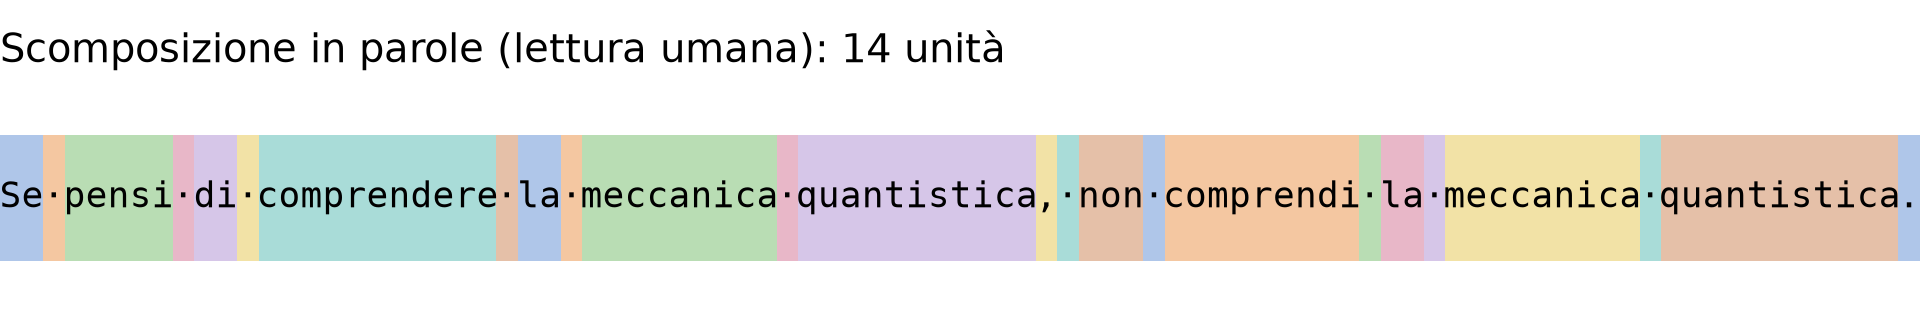
\includegraphics[width=\textwidth]{figure/cap2_scomposizione_parole.png}
  \caption{Scomposizione in parole. Ogni blocco è un'unità dotata di
  significato autonomo; il punto mediano segnala gli spazi.}
  \label{fig:scomp-parole}
\end{figure}

Per un modello linguistico la stessa frase si scompone invece come nella
Figura~\ref{fig:scomp-token}.

\begin{figure}[htbp]
  \centering
  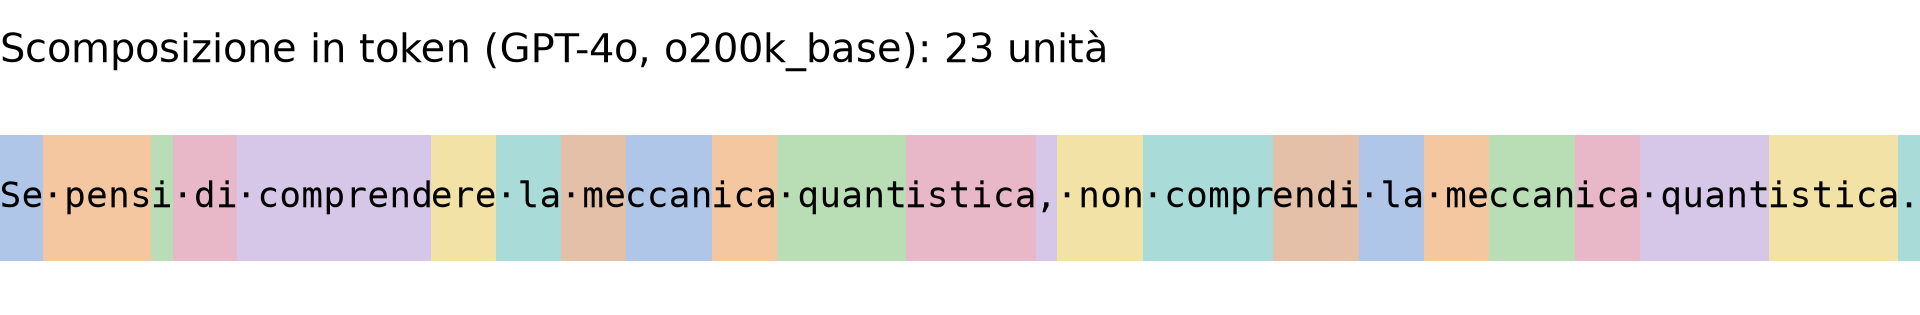
\includegraphics[width=\textwidth]{figure/cap2_scomposizione_token.png}
  \caption{Scomposizione in token della stessa frase, ottenuta con il
  tokenizzatore \texttt{o200k\_base} impiegato da GPT-4o. Le unità sono
  ventitré, non coincidono con le parole e in generale non hanno significato
  autonomo.}
  \label{fig:scomp-token}
\end{figure}

La frase non è divisa né in lettere né in parole, ma in gruppi di lettere
chiamati \emph{token}. Alcuni token coincidono con parole intere
(\texttt{·la}, \texttt{·non}), altri sono frammenti privi di significato
(\texttt{ccan}, \texttt{istica}). Si osservi in particolare la coppia
\emph{comprendere} e \emph{comprendi}: la prima si scompone in
\texttt{·comprend} e \texttt{ere}, la seconda in \texttt{·compr} e
\texttt{endi}. Due forme della stessa radice vengono dunque tagliate in punti
diversi, e il modello non riceve alcuna indicazione esplicita del fatto che
condividano la radice. Lo spazio, inoltre, non separa i token ma vi è
incorporato: la maggior parte dei token inizia con uno spazio, e la
segmentazione del testo in unità precede logicamente qualunque nozione di
parola.

La conversione avviene tramite un algoritmo detto \emph{tokenizzatore}, che
traduce un testo scritto in una qualsiasi lingua e in un qualsiasi alfabeto in
una sequenza di token estratti da un dizionario ampio ma finito, costruito una
volta per tutte a partire da un grande corpus. I dizionari dei tokenizzatori
più diffusi hanno dimensioni dell'ordine di $10^5$ elementi: quello di GPT-4o,
\texttt{o200k\_base}, ne conta \num{200019}; \texttt{cl100k\_base}, impiegato
come unità di analisi nei capitoli sperimentali per le ragioni discusse nel
Capitolo~\ref{cap:metodi}, ne conta \num{100277}; i modelli Qwen2.5 analizzati
in questa tesi ne condividono uno di circa \num{151000} voci. Poiché il
dizionario è finito ma le lingue possibili sono molte, i testi nelle lingue
meno rappresentate nel corpus di costruzione vengono frammentati in un numero
di token assai maggiore rispetto all'inglese.

Proprio come le parole per gli esseri umani, per un modello linguistico sono i
token a trasportare significato. Il significato non è però un'etichetta
associata al token, bensì una posizione: tramite un'operazione detta
\emph{embedding} ogni token viene mappato in un vettore di uno spazio a molte
dimensioni, e la geometria di quello spazio codifica le relazioni fra i token.
Vettori vicini corrispondono a token che compaiono in contesti simili, e
direzioni ricorrenti nello spazio corrispondono a relazioni ricorrenti nel
linguaggio.

La Figura~\ref{fig:embedding} mostra la proprietà su un caso concreto. I vettori
di trenta parole inglesi, appartenenti a cinque famiglie semantiche, sono
proiettati sulle prime due componenti principali dello spazio: le parole di
ciascuna famiglia si dispongono in gruppi distinti, benché la costruzione dei
vettori non abbia mai fatto uso di alcuna classificazione semantica, ma soltanto
delle co-occorrenze osservate in un corpus.

\begin{figure}[htbp]
  \centering
  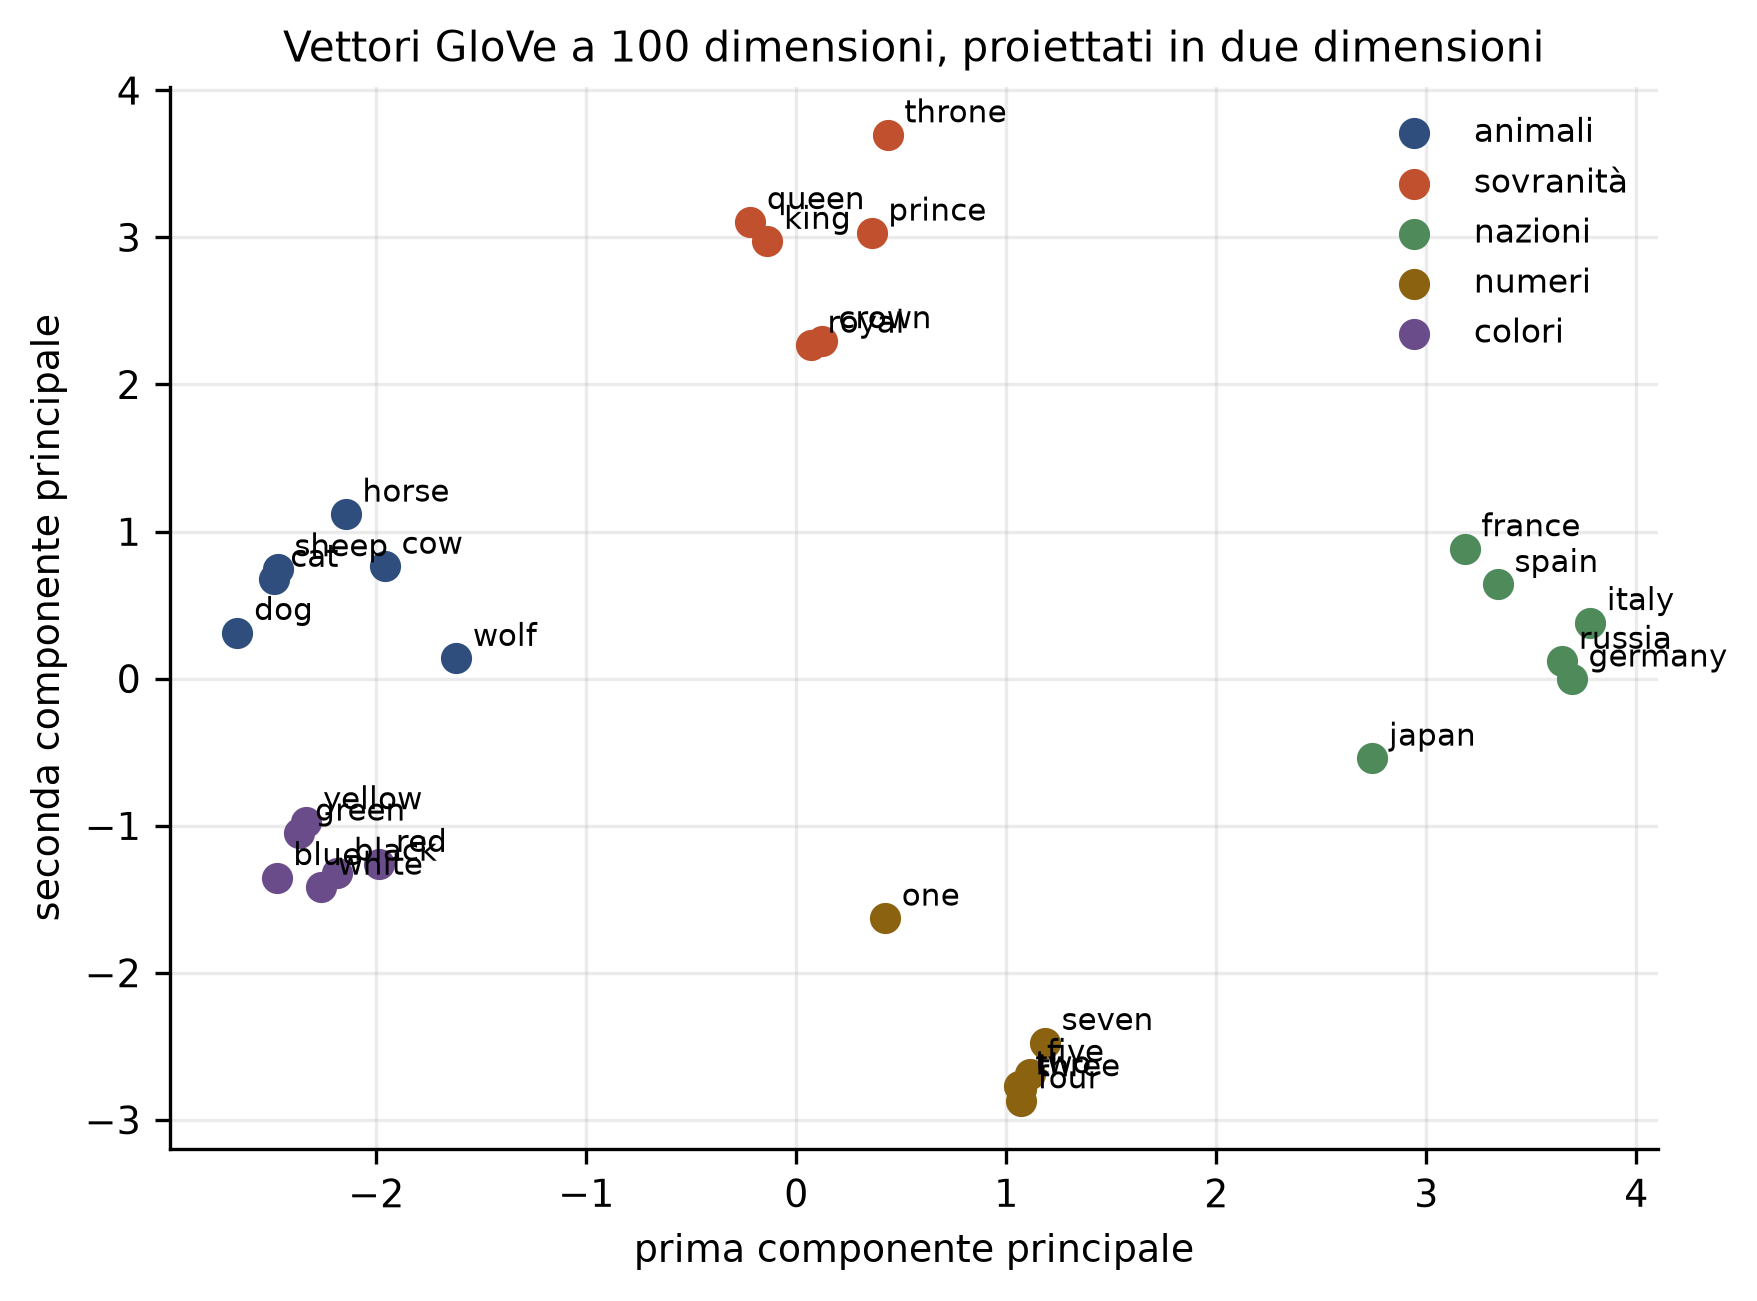
\includegraphics[width=0.82\textwidth]{figure/cap2_embedding_2d.png}
  \caption{Trenta parole inglesi rappresentate dai rispettivi vettori GloVe a
  100 dimensioni, proiettati sulle prime due componenti principali. Le cinque
  famiglie semantiche formano gruppi separati senza che alcuna informazione
  semantica sia stata fornita all'algoritmo. La proiezione conserva soltanto una
  parte della struttura, poiché riduce cento dimensioni a due: la vicinanza
  visibile in figura è una condizione sufficiente, non necessaria, alla
  vicinanza nello spazio originario.}
  \label{fig:embedding}
\end{figure}

I due spazi vettoriali che compaiono in questo lavoro hanno natura diversa. Ogni modello linguistico possiede una propria matrice di embedding,
appresa durante l'addestramento insieme a tutti gli altri parametri, e i cui
vettori non sono direttamente confrontabili fra modelli diversi: fra i modelli
analizzati in questa tesi la dimensione di tale spazio passa da 1536 per il
modello da 1.5 miliardi di parametri a 5120 per quello da 14 miliardi. Gli embedding impiegati nelle analisi di
questa tesi sono invece vettori GloVe a 100 dimensioni, pre-addestrati su un
corpus esterno e identici per tutti i testi esaminati: la scelta è dettata dalla
necessità di misurare i testi generati da modelli diversi con lo stesso metro, e
segue l'impostazione di~\cite{mikhaylovskiy2025states}. Nel
§\ref{sec:traiettoria} tali vettori verranno usati per trasformare un testo in
una traiettoria nello spazio semantico e studiarne l'autocorrelazione.


% ---------------------------------------------------------------------
\section{Generazione autoregressiva e temperatura}
\label{sec:temperatura}

Un modello linguistico autoregressivo, data una sequenza di token $t_{1:m}$,
sceglie il token successivo estraendolo da una distribuzione di probabilità che
dipende dalla sequenza stessa. La probabilità dell'intera sequenza si
decompone per mezzo della regola della catena,
\begin{equation}
  P(t_{1:m}) \;=\; \prod_{k=1}^{m} P(t_k \mid t_{1:k-1}),
  \label{eq:autoregressivo}
\end{equation}
e il modello è addestrato ad approssimare i singoli fattori
$P(t_k \mid t_{1:k-1})$, cioè a prevedere ogni token a partire da tutti quelli
che lo precedono. La generazione consiste nell'applicare ripetutamente questa
previsione, aggiungendo di volta in volta il token estratto alla sequenza che
condiziona l'estrazione successiva.

\paragraph{Origine della distribuzione condizionata.}
Il modo in cui il modello costruisce $P(t_k \mid t_{1:k-1})$ è ciò che
distingue le architetture moderne da quelle precedenti, ed è rilevante per
questo lavoro. I modelli oggi in uso si basano sull'architettura
\emph{transformer}~\cite{vaswani2017}, il cui elemento caratteristico è il
meccanismo di \emph{attenzione}. In esso ogni posizione della sequenza calcola
un peso per ciascuna delle posizioni precedenti e costruisce la propria
rappresentazione come combinazione pesata di quelle: il token in posizione $k$
può quindi attingere direttamente a qualunque token precedente, per lontano che
sia, senza che l'informazione debba propagarsi attraverso le posizioni
intermedie.

È una differenza sostanziale rispetto ai modelli ricorrenti, in cui
l'informazione proveniente da una posizione lontana deve attraversare tutte
quelle interposte e si degrada di conseguenza. Nel transformer il cammino fra
due posizioni qualsiasi ha lunghezza costante, e questo rende l'architettura in
linea di principio capace di rappresentare dipendenze fra porzioni di testo
molto distanti fra loro. È il meccanismo che, negli attuali modelli, potrebbe
dare origine alle correlazioni a lungo raggio descritte nel §\ref{sec:lrc}, e
una delle ragioni per cui ha senso cercarle nel testo generato. La capacità di
rappresentare tali dipendenze non implica però che il modello le riproduca
effettivamente, e l'attenzione opera comunque entro una finestra di contesto
finita: stabilire se le correlazioni siano presenti nel
testo prodotto resta una questione empirica, ed è precisamente quella affrontata
nei capitoli sperimentali.

\paragraph{Temperatura.}
Il modello non produce direttamente probabilità, ma valori reali detti
\emph{logit}, indicati con $u_1,\dots,u_{|\mathcal{L}|}$, uno per ciascun
elemento del dizionario $\mathcal{L}$. Essi vengono convertiti in distribuzione
di probabilità da una funzione softmax riscalata da un parametro
$T$~\cite{ackley1985}:
\begin{equation}
  p(t = \mathcal{L}_l \mid t_{1:i-1}) \;=\;
  \frac{\exp(u_l / T)}{\sum_{l'} \exp(u_{l'} / T)} .
  \label{eq:softmax}
\end{equation}

Il parametro $T$ prende il nome di temperatura, e la denominazione non è una
semplice analogia. Ponendo $E_l = -u_l$, la~\eqref{eq:softmax} coincide con la
distribuzione di Boltzmann $p_l \propto e^{-E_l/T}$ di un sistema a
$|\mathcal{L}|$ stati in equilibrio termico alla temperatura $T$. Questa
identificazione è ciò che giustifica la ricerca, nel testo generato, dei
fenomeni caratteristici dei sistemi termodinamici, e in particolare delle
transizioni di fase discusse nel §\ref{sec:fasi}.

I due limiti sono immediati. Per $T\to0$ la distribuzione si concentra sul token
di logit massimo e la generazione diventa deterministica; per $T\to\infty$ tende
alla distribuzione uniforme sull'intero dizionario, indipendentemente dal
contesto. Fra i due estremi, valori $T<1$ concentrano la massa di probabilità
sugli eventi più probabili, mentre valori $T>1$ la ridistribuiscono verso quelli
meno probabili. La temperatura non modifica dunque ciò che il modello ha
appreso, ma soltanto quanto fedelmente la generazione segue la distribuzione
appresa.

Nella pratica corrente la generazione impiega anche il troncamento della
distribuzione, nelle varianti top-$k$~\cite{fan2018} e
top-$p$~\cite{holtzman2020}, e penalità che scoraggiano la ripetizione. Tutti
questi meccanismi agiscono sulla stessa distribuzione e introducono un secondo
parametro d'ordine, rendendo impossibile attribuire alla sola temperatura il
comportamento osservato. Per questa ragione, e coerentemente con la scelta
esplicita di~\cite{mikhaylovskiy2025zipf}, i dati analizzati in questa tesi sono
stati generati impiegando il solo campionamento per temperatura.


% ---------------------------------------------------------------------
\section{Fasi e stato critico}
\label{sec:fasi}

Una fase di un sistema fisico è uno stato, tipicamente di equilibrio, dotato di
proprietà macroscopiche caratteristiche e stabile in una regione dello spazio
dei parametri; alla frontiera di tali regioni avviene una transizione di fase.
Secondo la classificazione di Ehrenfest~\cite{ehrenfest1933} una transizione di
ordine $n$ è una discontinuità nella derivata $n$-esima dell'energia libera.

Applicare alla lettera questa classificazione al testo generato non è però
possibile. Il sistema considerato non ha un'energia libera di cui prendere
derivate, non è in equilibrio con alcun bagno termico e
non possiede un limite termodinamico, poiché il numero di token di un documento
resta finito. Ciò che rende legittimo il linguaggio delle fasi è la
corrispondenza stabilita nel §\ref{sec:temperatura}: la~\eqref{eq:softmax}
coincide con una distribuzione di Boltzmann in cui i logit giocano il ruolo di
energie e il parametro di campionamento quello di temperatura. La distribuzione
condizionata da cui ogni token viene estratto è dunque, letteralmente, una
distribuzione di Gibbs, e $T$ ne è la temperatura. Quello che resta analogia, e
non identità, è il passaggio dal singolo token al documento: nulla garantisce
che le proprietà collettive di una sequenza generata token per token si
comportino come le proprietà macroscopiche di un sistema all'equilibrio. Il
vocabolario di Ehrenfest viene perciò impiegato in senso descrittivo, per
nominare regioni di comportamento qualitativamente diverso separate da
variazioni rapide, e non per rivendicare una transizione di fase in senso
termodinamico.

Ciò che rende il concetto utile è il comportamento nel punto critico che
separa due fasi: là le correlazioni decadono a legge di potenza e la loro
portata diverge, e molte grandezze osservabili esibiscono lo stesso andamento.
Il criterio inverso, per cui dove compare una legge di potenza si sospetta uno
stato critico, va maneggiato con prudenza, perché distribuzioni a legge di
potenza si generano in molti modi che con la criticità non hanno rapporto, dal
semplice prodotto di variabili aleatorie ai processi di preferential
attachment. Preso da solo, l'andamento a legge di potenza di una quantità non
dimostra nulla. Acquista forza quando più osservabili indipendenti cambiano
regime allo stesso valore del parametro di controllo, ed è in questa forma che
viene impiegato nel §\ref{sec:tstar}: non la legge di potenza di una misura,
ma la convergenza di criteri costruiti per scopi diversi.

Il quadro è stato applicato ai modelli linguistici in~\cite{nakaishi2024}, dove
la temperatura di campionamento separa una fase a bassa temperatura,
caratterizzata da strutture ripetitive, da una ad alta temperatura in cui il
testo è incomprensibile. La tesi sostenuta in quel lavoro è che il linguaggio
naturale si collochi \emph{sul} punto critico fra le due: nello spazio dei
processi stocastici che generano successioni di simboli, il processo
corrispondente a una lingua naturale giacerebbe sulla superficie critica che
separa le due regioni, e un modello addestrato su quella lingua definisce una
famiglia di processi che quella superficie attraversa al variare di $T$. Il
risultato è verificato su modelli da 160 milioni a 2.8 miliardi di parametri, su
sei lingue e su due diverse mappature del testo in successione numerica, il che
ne stabilisce l'indipendenza dalla scala e dalla lingua.

Questa congettura è il punto di contatto più stretto fra il presente lavoro e la
letteratura di fisica statistica sull'argomento, e il
Capitolo~\ref{cap:risultati1} ne fornisce una verifica indipendente: se il
linguaggio naturale è critico, allora la temperatura alla quale il testo
generato somiglia di più a quello umano deve coincidere con quella alla quale il
modello attraversa la transizione, e criteri che misurano proprietà diverse
devono indicarla concordemente.


% ---------------------------------------------------------------------
\subsection{La traiettoria di embedding}
\label{sec:traiettoria}

Il §\ref{sec:token} ha introdotto i vettori di embedding come rappresentazione
del significato. Applicandoli a un testo si ottiene un oggetto geometrico: detta
$(p_1,\dots,p_M)$ la successione delle parole del documento e $v(\cdot)$ la
mappa che associa a una parola il proprio vettore, si pone
\begin{equation}
  \mathbf{m}_i \;=\;
  \begin{cases}
    v(p_i) - \bar{v} & \text{se $p_i$ ha un vettore},\\[2pt]
    \mathbf{0}       & \text{altrimenti},
  \end{cases}
  \label{eq:traiettoria}
\end{equation}
dove $\bar{v}$ è la media dei vettori delle sole parole che ne possiedono uno.
La successione $(\mathbf{m}_1,\dots,\mathbf{m}_M)$ è la traiettoria del testo
nello spazio degli embedding: ogni parola è un punto, e leggere il documento
dall'inizio alla fine equivale a percorrere quella traiettoria.

Due dettagli della~\eqref{eq:traiettoria} incidono sui risultati. Il primo è la
centratura: sottrarre $\bar{v}$ elimina la
direzione media del documento, che altrimenti dominerebbe ogni prodotto scalare
e renderebbe tutte le coppie di parole artificialmente simili. Il secondo è il
trattamento delle parole prive di vettore, alle quali si assegna il vettore
nullo \emph{dopo} la centratura, seguendo~\cite{mikhaylovskiy2025states}: la
posizione nella successione viene così conservata, e con essa la struttura dei
lag, ma la parola non contribuisce ad alcuna correlazione. La conseguenza è che
un testo in cui molte parole non hanno vettore produce una traiettoria fatta in
larga parte di zeri, e le misure che seguono perdono significato prima di
diventare incalcolabili: è la ragione della soglia di validità introdotta più
avanti.

Su questa successione si definisce l'autocorrelazione a distanza $\tau$ come
media della similarità coseno fra i vettori che distano $\tau$ posizioni,
\begin{equation}
  C(\tau) \;=\; \frac{1}{M-\tau} \sum_{i=1}^{M-\tau}
  \frac{\mathbf{m}_i \cdot \mathbf{m}_{i+\tau}}
       {\lVert \mathbf{m}_i \rVert \, \lVert \mathbf{m}_{i+\tau} \rVert},
  \label{eq:acf-embedding}
\end{equation}
con la convenzione che i termini in cui uno dei due vettori è nullo
contribuiscono zero. La~\eqref{eq:acf-embedding} risponde alla domanda: due
parole che distano $\tau$ posizioni tendono a essere semanticamente affini? Vale
$C(\tau) \simeq 0$ quando non c'è alcuna relazione, ed è tanto più vicina a uno
quanto più il testo, a quella distanza, torna a parlare della stessa cosa.

Poiché la~\eqref{eq:acf-embedding} resta calcolabile su qualunque successione,
serve un riferimento che dica quale ampiezza sia distinguibile dal caso. Si
adotta il rimescolamento: si permutano a caso le posizioni della traiettoria, si
ricalcola $C(\tau)$ e si prende il massimo del suo modulo. Il valore così
ottenuto è il livello di rumore del documento, ed è la stessa costruzione dei
null model del §\ref{sec:null}: conserva il contenuto e distrugge l'ordine.
Un'autocorrelazione la cui ampiezza non superi quel livello non è distinguibile
da una successione di parole senza struttura.


% ---------------------------------------------------------------------
\subsection{Le tre fasi}
\label{sec:tre-fasi}

Applicando questo linguaggio al testo generato,
in~\cite{mikhaylovskiy2025states} vengono individuate tre fasi, distinte dal
comportamento di $C(\tau)$.

A bassa temperatura il testo degenera in cicli di ripetizione: la traiettoria
ripassa periodicamente per gli stessi punti, $C(\tau)$ oscilla con periodo pari
alla lunghezza del ciclo e la sua trasformata di Fourier presenta picchi netti.
La quantità che segnala il fenomeno è quindi
\begin{equation}
  \Phi \;=\; \max_{k \ge 1} \bigl\lvert \hat{C}_k \bigr\rvert ,
  \label{eq:periodicita}
\end{equation}
dove $\hat{C}_k$ sono i coefficienti della trasformata discreta di $C(\tau)$. Il
coefficiente $k = 0$ viene escluso perché proporzionale alla media di $C(\tau)$,
cioè al livello complessivo di correlazione e non alla sua periodicità: un testo
uniformemente correlato ma non ciclico ha $\hat{C}_0$ grande e tutti gli altri
coefficienti piccoli. Questa è la fase che, per analogia con gli stati della
materia, viene detta solida. È lo stesso regime in cui, come osservato nel
§\ref{sec:ponte}, la fluttuazione della DFA satura e $\alpha_{\mathrm{DFA}}$
scende verso zero: le due misure segnalano lo stesso fenomeno da due angolazioni
diverse.

La~\eqref{eq:periodicita} si comporta come un parametro d'ordine nel senso che
assume valori grandi in una fase e piccoli nell'altra, ma non si annulla
identicamente fuori dalla fase periodica: su una successione priva di struttura
resta un valore residuo dovuto alle fluttuazioni campionarie. Il
Capitolo~\ref{cap:risultati1} riporta di conseguenza il suo crollo in termini di
ordini di grandezza e non di annullamento.

In una finestra ristretta di temperature $C(\tau)$ decade invece a legge di
potenza: è lo stato critico, quello in cui le leggi di Zipf e di Heaps
introdotte nel §\ref{sec:scala} risultano meglio soddisfatte. Ad alta
temperatura, infine, le correlazioni decadono esponenzialmente e non sussiste
struttura a lungo raggio: è la fase detta amorfa, o gassosa.

Per distinguere le ultime due fasi vengono confrontati due fit
dell'autocorrelazione, uno a legge di potenza e uno esponenziale, tramite il
rapporto dei rispettivi errori~\cite{mikhaylovskiy2023}:
\begin{equation}
  \mathrm{GAPELMAPER} \;=\;
  \frac{\mathrm{MAPE}\bigl(\text{fit a legge di potenza}\bigr)}
       {\mathrm{MAPE}\bigl(\text{fit esponenziale}\bigr)},
  \label{eq:gapelmaper}
\end{equation}
dove il MAPE è quello definito nella~\eqref{eq:mape}. Il rapporto è minore di 1
quando il fit a legge di potenza descrive i dati meglio di quello esponenziale,
e segnala quindi lo stato critico; è maggiore di 1 nella fase amorfa.

La~\eqref{eq:gapelmaper} è un rapporto fra errori di fit, e come tale resta
calcolabile anche quando l'autocorrelazione è indistinguibile dal rumore; in
quel regime, però, il suo valore è privo di contenuto informativo, perché
entrambi i fit descrivono male dati che non contengono alcun segnale.

Le tre fasi, la soglia di periodicità e la condizione di validità si compongono
nella regola seguente. Detti $\kappa$ la quota di parole del documento dotate di
un vettore, $A = \max_\tau \lvert C(\tau)\rvert$ l'ampiezza
dell'autocorrelazione e $\eta$ il livello di rumore stimato per rimescolamento,
un documento viene classificato come
%
\begin{itemize}
  \item \emph{non valutabile}, se $\kappa < \kappa_{\min}$ oppure $A \le \eta$;
  \item \emph{solido}, altrimenti, se $\Phi > \Phi_{\min}$;
  \item \emph{critico}, altrimenti, se $\mathrm{GAPELMAPER} < 1$;
  \item \emph{amorfo} in ogni altro caso.
\end{itemize}
%
L'ordine dei controlli non è indifferente. La condizione di validità viene per
prima perché le altre due misure, su un documento che non la supera, sono numeri
senza referente; la periodicità viene prima del GAPELMAPER perché
un'autocorrelazione periodica non è né una legge di potenza né un esponenziale,
e sottoporla a quel confronto restituirebbe un valore arbitrario. I due valori
di soglia sono fissati nel Capitolo~\ref{cap:risultati1}, dove ne vengono
discussi l'origine e l'effetto.

I due quadri di riferimento non coincidono del tutto.
In~\cite{nakaishi2024} le fasi sono due e ciò che le separa è un punto critico,
cioè un insieme di misura nulla nello spazio dei parametri;
in~\cite{mikhaylovskiy2025states} lo stato critico diventa invece una fase a sé,
dotata di estensione finita. La differenza non è terminologica: nel primo caso
attraversare la transizione con uno sweep a passo finito significa quasi
certamente saltare il punto critico, nel secondo significa attraversare una
regione che si può campionare. Il Capitolo~\ref{cap:risultati1} riporta i dati
pertinenti alla questione senza pretendere di risolverla.


% ---------------------------------------------------------------------
\section{Notazione}
\label{sec:notazione}

Le grandezze introdotte in questo capitolo provengono da lavori che adottano
simboli in conflitto fra loro. La Tabella~\ref{tab:notazione} raccoglie la
notazione seguita in questa tesi, che viene mantenuta senza eccezioni nei
capitoli successivi.

\begin{table}[htbp]
\centering
\small
\begin{tabular}{@{}l>{\raggedright\arraybackslash}p{8.3cm}c@{}}
\toprule
Simbolo & Grandezza & Definita in \\
\midrule
\multicolumn{3}{@{}l}{\itshape Testo e vocabolario} \\
$\mathbf{W}$, $w_t$, $N$ & sequenza di parole, parola in posizione $t$, lunghezza & \eqref{eq:sequenza} \\
$\mathcal{D}$, $\mathcal{D}(t)$ & dizionario e dizionario parziale & §\ref{sec:scala} \\
$f(r)$, $\alpha$ & frequenza della parola di rango $r$, esponente di Zipf & \eqref{eq:zipf} \\
$\gamma_H$ & esponente di Heaps & \eqref{eq:heaps} \\
$R$ & parole nuove nella seconda metà, rapportate alla prima & \eqref{eq:R} \\
MAPE & errore percentuale assoluto medio del fit & \eqref{eq:mape} \\
\addlinespace
\multicolumn{3}{@{}l}{\itshape Correlazioni} \\
$x_k$ & successione binaria generata da un osservabile & \eqref{eq:osservabile} \\
$c(s)$, $\theta$ & autocorrelazione a distanza $s$ e suo esponente di decadimento & \eqref{eq:acf-power} \\
$X(t)$, $\sigma_X^2$, $\gamma$ & conteggio, sua varianza, esponente di crescita & \eqref{eq:sigma} \\
$F(s)$, $\alpha_{\mathrm{DFA}}$ & fluttuazione detrendizzata e suo esponente & \eqref{eq:dfa-alpha} \\
\addlinespace
\multicolumn{3}{@{}l}{\itshape Intervalli e burstiness} \\
$\tau_i$, $p(\tau)$ & intervalli fra occorrenze e loro distribuzione & §\ref{sec:burst} \\
cv, $B$ & coefficiente di variazione, indice di Goh--Barabási & \eqref{eq:cv}, \eqref{eq:goh} \\
$S(0)$, $c_\tau(k)$ & spettro a frequenza nulla, autocorrelazione degli intervalli & \eqref{eq:eq4} \\
$\hat\gamma_{A1}$, $\hat\gamma_{A2}$ & esponenti misurati sui due null model & §\ref{sec:null} \\
$q$ & quota di burstiness & \eqref{eq:quota} \\
$\mu$, $\tau_c$ & esponente di coda e cut-off di $p(\tau)$ & \eqref{eq:troncata} \\
$J$ & entropia degli intervalli, riferita al processo di Poisson & \eqref{eq:entropia-intervalli} \\
\addlinespace
\multicolumn{3}{@{}l}{\itshape Entropia e compressione} \\
$H$, $h$ & entropia di Shannon, tasso di entropia & \eqref{eq:H-singola}, \eqref{eq:tasso-entropia} \\
$c(x|y)$, $h(x|y)$ & frasi del cross-parsing, cross-entropia stimata & \eqref{eq:crossparsing} \\
$D(x\|y)$, $D_s$ & divergenza di Kullback--Leibler e sua versione simmetrizzata & \eqref{eq:kl}, \eqref{eq:kl-sym} \\
$C(x)$, $R_{\mathrm{gzip}}$ & dimensione compressa e rapporto di compressione & \eqref{eq:cratio} \\
NCD & distanza normalizzata di compressione & \eqref{eq:ncd} \\
\addlinespace
\multicolumn{3}{@{}l}{\itshape Generazione e fasi} \\
$u_l$, $T$ & logit del token $l$, temperatura di campionamento & \eqref{eq:softmax} \\
$C(\tau)$ & autocorrelazione della traiettoria di embedding & \eqref{eq:acf-embedding} \\
$\Phi$ & parametro di periodicità di $C(\tau)$ & \eqref{eq:periodicita} \\
GAPELMAPER & rapporto fra gli errori dei due fit dell'autocorrelazione & \eqref{eq:gapelmaper} \\
$N_{\mathrm{eff}}$ & lunghezza comune di analisi & §\ref{sec:scelte} \\
\bottomrule
\end{tabular}
\caption{Notazione adottata in questa tesi.}
\label{tab:notazione}
\end{table}

Per tre simboli la scelta operata qui si discosta da quella di almeno una delle
fonti; la Tabella~\ref{tab:collisioni} riassume le corrispondenze.

\begin{center}
\small
\begin{tabular}{@{}lcccc@{}}
\toprule
Grandezza & Qui & \cite{mikhaylovskiy2025zipf} & \cite{lippi2019} & \cite{altmann2012} \\
\midrule
Esponente di Zipf                  & $\alpha$                & $\alpha$ & $\beta$  & --- \\
Esponente di Heaps                 & $\gamma_H$              & $\beta$  & $\nu$    & --- \\
Esponente della fluttuazione (DFA) & $\alpha_{\mathrm{DFA}}$ & ---      & $\alpha$ & --- \\
Decadimento dell'autocorrelazione  & $\theta$                & ---      & $\gamma$ & $\beta$ \\
Crescita della varianza del conteggio & $\gamma$             & ---      & ---      & $\gamma$ \\
Rapporto di compressione           & $R_{\mathrm{gzip}}$     & ---      & ---      & --- \\
\bottomrule
\end{tabular}
\captionof{table}{Corrispondenza fra la notazione adottata e quella delle fonti primarie,
limitatamente ai simboli per cui le fonti divergono. Il rapporto di compressione
è indicato con $R(x)$ in~\cite{hadad2026}, dove però $R$ non ha il significato
che assume qui.}
\label{tab:collisioni}
\end{center}

Il simbolo $\alpha$ è riservato all'esponente di Zipf, come
in~\cite{mikhaylovskiy2025zipf}, mentre l'esponente della detrended
fluctuation analysis, indicato con $\alpha$ in~\cite{lippi2019}, riceve il
pedice $\mathrm{DFA}$. L'esponente di Heaps è indicato con $\gamma_H$ anziché
con $\beta$ o $\nu$, per lasciare $\gamma$ libero per l'esponente di crescita
della varianza del conteggio, che è la convenzione di~\cite{altmann2012} e
della seconda parte sperimentale. Il decadimento dell'autocorrelazione riceve
infine il simbolo $\theta$, che nessuna delle fonti impiega, poiché entrambe
le lettere che gli sono attribuite in letteratura sono già assegnate. La
lettera $R$ resta al descrittore di~\cite{mikhaylovskiy2025zipf} e il rapporto
di compressione riceve il pedice $\mathrm{gzip}$.

Valgono inoltre le convenzioni seguenti, usate nel seguito senza ulteriore
avviso. Il circonflesso indica una quantità stimata dai dati in contrapposizione
al corrispondente valore teorico, come in $\hat\gamma$. I pedici $A1$ e $A2$
indicano i due null model del §\ref{sec:null}. Il simbolo $|\cdot|$ applicato a
un insieme ne indica la cardinalità e applicato a un testo la lunghezza, in
parole o in byte secondo il contesto. Le medie sono indicate con
$\langle\cdot\rangle$ e si intendono calcolate sull'intero documento salvo
diversa indicazione.
